% Copyright (C) 2014 by Thomas Auzinger <thomas.auzinger@cg.tuwien.ac.at>

\documentclass[draft,final]{vutinfth} % Remove option 'final' to obtain debug information.

% Extended LaTeX functionality is enables by including packages with \usepackage{...}.
\usepackage{fixltx2e}  % Provides fixes for several errors in LaTeX2e.
\usepackage[normalem]{ulem}
\usepackage{amsmath}   % Extended typesetting of mathematical expression.
\usepackage{amssymb}   % Provides a multitude of mathematical symbols.
\usepackage{mathtools} % Further extensions of mathematical typesetting.
\usepackage{microtype} % Small-scale typographic enhancements.
\usepackage{enumitem}  % User control over the layout of lists (itemize, enumerate, description).
\usepackage{multirow}  % Allows table elements to span several rows.
\usepackage{booktabs}  % Improves the typesettings of tables.
\usepackage[ruled,linesnumbered,algochapter]{algorithm2e} % Enables the writing of pseudo code.
\usepackage{color,soul}
\usepackage{verbatim}
\usepackage{gensymb}
\usepackage{listings}
\usepackage{tikz}		% Diagram extension for hierarchical edge bundle
\usepackage{menukeys}	% Keyboard symbols
\usepackage{nag}       % Issues warnings when best practices in writing LaTeX documents are violated.
\usepackage{hyperref}  % Enables cross linking in the electronic document version. This package has to be included second to last.
\usepackage[acronym,toc]{glossaries} % Enables the generation of glossaries and lists fo acronyms. This package has to be included last.

\setsecnumdepth{subsection} % enumerate subsections

% Use an optional index
\makeindex
% Use an optional glossary
\makeglossaries
%\glstocfalse % remove the glossaries from the table of contents

% Set persons with 4 arguments:
%  {title before name}{name}{title after name}{gender}
%  where both titles are optional (i.e. can be given as empty brackets {})
\setauthor{}{Mario Gastegger}{}{male}
\setadvisor{Ao.Univ.Prof. Dipl.-Ing. Dr.techn.}{Martin Ertl}{}{male}

% For bachelor and master theses
\setfirstassistant{}{}{}{male}
\setsecondassistant{}{}{}{male}
\setthirdassistant{}{}{}{male}

% For dissertations
\setfirstreviewer{}{}{}{male}
\setsecondreviewer{}{}{}{male}

% For dissertations at the PhD School
\setsecondadvisor{}{}{}{male}

% Required data
\setaddress{Ameisgasse 15/9, 1140 Wien}
\setregnumber{0726289}
\setdate{23}{09}{2015}
\settitle{Program understanding in Gforth/Forth}{Program understanding in Gforth/Forth} % sets English and German version of the title (both can be English or German)
\setsubtitle{Applicability of existing graphical approaches}{Applicability of existing graphical approaches} % sets English and German version of the subtitle (both can be English or German)

% Select the thesis type: bachelor / master / doctor / phd-school
% Bachelor:
\setthesis{bachelor}
%
% Master:
%\setthesis{master}
%\setmasterdegree{dipl.} % dipl. / rer.nat. / rer.soc.oec. / master
%
% Doctor:
%\setthesis{doctor}
%\setdoctordegree{rer.soc.oec.}% rer.nat. / techn. / rer.soc.oec.
%
% Doctor at the PhD School
%\setthesis{phd-school} % Deactivate non-English title pages (see below)

% For bachelor and master
\setcurriculum{Software \& Information Engineering}{Software \& Information Engineering} % sets the English and German name of the curriculum

% For dissertations at the PhD School
\setfirstreviewerdata{Affiliation, Country}
\setsecondreviewerdata{Affiliation, Country}


\begin{document}

\frontmatter % switches to roman numbering
% The structure of the thesis has to conform to
%  http://www.informatik.tuwien.ac.at/dekanat

\addtitlepage{naustrian} % German title page (not for dissertations at the PhD School)
\addtitlepage{english} % English title page
\addstatementpage

%\begin{danksagung*}
%Ihr Text hier.
%\end{danksagung*}

%\begin{acknowledgements*}
%Enter your text here.
%\end{acknowledgements*}

%\begin{kurzfassung}
%Ihr Text hier.
%\end{kurzfassung}

\begin{abstract}
The topic of program understanding has been researched for the procedural and object oriented paradigm. But there exists nearly no work on program understanding for concatenative languages. This thesis aims to gain an overview on the existing methods to support program understanding in Gforth/Forth and to evaluate the applicability of existing graphical approaches for other paradigms on Gforth/Forth. The focus lies on methods for trace visualization.
The massive sequence view, the polymetric view and the memory access view are well applicable and helpful, while the hierarchic edge bundle and gfvis, the improvement for Gforth's dbg, turned out to be not as helpful as expected. The key to program understanding in Gforth/Forth lies in expressive naming, documentation (behavior and stack-effect) and short definitions.


%\begin{itemize}
% \item Kontext der Arbeit / Aufgabenstellung

%\item Fragestellung der Diplomarbeit

%\item Wissenschaftliche Methode(n) / Verfahrensweise(n), mit deren Hilfe die Ergebnisse erzielt wurden
%explorative qualitative

%\item Zentrale Ergebnisse der Arbeit
%\end{itemize}

\end{abstract}

% Select the language of the thesis, e.g., english or naustrian.
\selectlanguage{english}

% Add a table of contents (toc)
\tableofcontents % starred version, i.e., \tableofcontents*, removes the self-entry

% Use an optional list of figures
\listoffigures % starred version, i.e., \listoffigures*, removes the toc entry

% Use an optional list of tables
%\listoftables % starred version, i.e., \listoftables*, removes the toc entry

% Use an optional list of alogrithms
%\listofalgorithms
% \addcontentsline{toc}{chapter}{List of Algorithms}

% Switch to arabic numbering and start the enumeration of chapters in the table of content.
\mainmatter

\chapter{Introduction}

\section*{Motivation}

Software systems underlie continuous changes throughout their whole life cycle.
They evolve from the beginning of development until their release and maintenance phase. Large software systems\footnote{"The term large is, generally, used to describe software whose size in number of lines of code is greater than some arbitrary value. For reasons indicated in [leh79], it is more appropriate to define a large program as one developed by processes involving groups with two or more management levels."\cite{Lehman:2003:SEB:950401.950407}} and most of all, software  classified as type E \cite{Cook:2006:ESS:1115566.1115567}, get more complex over time.\\
If there are more than a few developers/development teams involved or the developers/development teams are spread all over the world, there exists more foreign code than self written code. This makes it necessary to understand foreign code.
Most of all when it comes to making changes, enhancements or fixes, there is a very high level of understanding of the software at hand necessary\cite{Boehm:1976:SE:1311958.1312684}\cite{Singer97anexamination}. Due to \cite{Cornelissen:2009:SSP:1638616.1639301}, "... up to 60\% of the maintenance effort is spent on gaining a sufficient understanding of the program ...". These facts emphasize the need for computer aided methods to improve program understanding.

This thesis addresses the task of improving program comprehension of the concatenative programming language Forth on several levels. The terms "program understanding" and "program comprehension" are considered synonym. Namely the reading of source code, static analysis, dynamic analysis and the assistance of writing readable and easy to understand source code.

Due to the nature of concatenative languages, it is possible to write source code which reads very similar to natural language. There are no hard boundaries to the structure of the source code(custom defined loops and control structures) as in most other languages. Since Forth directly operates only on stacks and memory, the information which is immediately needed to follow the program execution is limited to those structures. In contrast, in object-oriented languages there is also object state, object life cycle and concurrency to keep in mind.

\begin{comment}
\hl{mental model(LaToza et al., 2006) read: ..comment}
\@inproceedings\{Lieberman:1995:BGC:223904.223969,
author = \{Lieberman, Henry and Fry, Christopher\},
title = \{Bridging the Gulf Between Code and Behavior in Programming\},
booktitle = \{Proceedings of the SIGCHI Conference on Human Factors in Computing Systems\},
series = \{CHI '95\},
year = \{1995\},
isbn = \{0-201-84705-1\},
location = \{Denver, Colorado, USA\},
pages = \{480--486\},
numpages = \{7\},
url = \{http://dx.doi.org/10.1145/223904.223969\},
doi = \{10.1145/223904.223969\},
acmid = \{223969\},
publisher = \{ACM Press/Addison-Wesley Publishing Co.\},
address = \{New York, NY, USA\},
\}
\end{comment}


\section*{Problem statement}

There has been done plenty of work on the task of program comprehension in object oriented and procedural languages\cite{Cornelissen:2009:SSP:1638616.1639301}, but nearly none for concatenative languages. \begin{comment} The qualitative exploratory approach of this thesis does not encourage the formulation of specific hypothesis. Therefore the first question, is the applicability of existing methods and their visualization techniques. The second question to be answered, concerns new approaches, which may be exclusive to concatenative languages or Gforth/Forth.\end{comment}

\section*{Aim of the work}

This work aims to give a brief overview on the field of program comprehension and its methods, to show existing aids to program understanding in Gforth/Forth and to study the applicability of some existing analysis and visualization approaches for other paradigms. Furthermore the suggestion of new methods or the modification of existing methods to meet the characteristics of Gforth/Forth.

\section*{Structure of the work}

In Chapter \ref{chap:Methodology}, I will outline the methodological approach of this thesis. In Chapter \ref{chap:StateOfTheArt}, there will be a brief overview on the topic of program comprehension, an overview on the existing tools to improve program understanding in general and on those specific to Gforth/Forth and afterwards I will present a selection of visualization approaches for procedural and object-oriented languages. In Chapter \ref{chap:Results}, I will present some of the previously mentioned approaches for other paradigms applied to a real world Forth program, analyze their applicability and propose modifications to those approaches. Afterwards I will present a prototype implementation of a program trace visualization enhancement to Gforth. Chapter \ref{chap:Summary} concludes the thesis with a summary and topics of further investigation.

\begin{comment}
At first, the available information of a forth program is identified. The next step is to characterize the information and its necessity for program comprehension is investigated. The differences of forth and object oriented languages are summarized and then the applicability of existing analysis and visualization methods is presented. \hl{Since there is no standard implementation of object orientation if forth, this thesis won't take any object orientation implementation into account.}
The last part of this thesis investigates probable enhancements and modifications to existing methods and proposes new approaches.
After the conclusion, the thesis presents further suggestions to support program comprehension and further topics of research in this direction.
\end{comment}

\chapter{Methodology}

\section{used concepts}

\begin{itemize}
\item prototyping
\item reading codes
\item print-debugging
\item step-debugging
\end{itemize}

\section{methods and/or models}

\begin{itemize}
\item prototyping
\end{itemize}

\section{languages}

\begin{itemize}
\item postscript
\item forth
\item shell script
\item c
\item m2
\end{itemize}


\section{design methods}

?

\section{data models}

?

\section{analysis methods}

\begin{itemize}
\item reading code
\item tail and error
\end{itemize}

\section{formalisms}

?

\newglossaryentry{UML}
{
  name={Unified Modeling Language},
  description={The Unified Modeling Language provides a standard way for modeling artifacts of software engineering. See \url{http://www.uml.org/} for detailed information on UML.}
}

\newglossaryentry{GraphTrace}
{
  name={GraphTrace},
  description={This paper describes GraphTrace, a tool we have developed to assist in understanding object-oriented programs, GraphTrace allows a user to create displays revealing different aspects of the structure of an object-oriented program, and then to animate these displays in order to visually understand how the program works.}
}

\chapter{Analysis of existing approaches}
\label{chap:StateOfTheArt}

The focus here lies on so called E type software systems. E stands for evolving \cite{Cook:2006:ESS:1115566.1115567}, most of the real world software systems are type E. These systems are of particular interest since they underlie continuous changes throughout their whole life cycle. Thus understanding existing code, which might not be well documented, is crucial for the maintenance of those systems.

\section{Program comprehension}

Program comprehension can be gained through several approaches. First of all, reading the code.
In \cite{Basili:1997:EPR:257260.257262}, Basili et al. approach the concept of reading on a very fundamental level. The natural way to learn writing, is to learn to read first. The reading then forms a model for our writing.  His research shows that reading is most effective compared to testing. This suggests, that readability of code does impact the efficiency of failure discovery. According to Basili et al., the most severe problem is the fact that programming languages are learned the other way round. We first learn to write code and then learn to read it. Furthermore, the ability to read code is not properly addressed in education. The syntactical flexibility, Forth provides compared to other languages(and paradigms), allows it to achieve a very natural seeming reading experience. Thus our skills in natural languages could become in handy and make program reading and thus understanding even more efficient. This would in the end result in higher code quality in terms of failures and unexpected or unintended behavior.

There emerged several strategies on how to read and understand a program\cite{Storey:1999:CDE:308936.308940}\cite{Storey:1997:PUT:832304.836998}:
\subsubsection*{Top down program comprehension}
Using the top down strategy, the reader begins on the highest level of abstraction, the main purpose of the program and then builds a hierarchy by refining it into sub tasks until the lowest level of abstraction is reached.
\subsubsection*{Bottom up program comprehension} Using the bottom up strategy, the reader builds the mental model by grouping low level parts of code building high levels abstraction until the whole program is understood.
\subsubsection*{Knowledge based program comprehension} The knowledge based strategy, allows both, the bottom up and the top down approach. The assumption is, that programmers have a certain mental model of the software, this model is evolved by both refinement and abstraction.
\subsubsection*{Systematic and as-needed program comprehension} This strategy embodies detailed reading as well as only focusing on the code necessary to fulfill the task at hand.
\subsubsection*{Integrated approaches of program comprehension} This strategy allows freely switching between the top down, the bottom up and the knowledge based approach.
\\\\
As Storey et al.\cite{Storey:1999:CDE:308936.308940} points out, there are certain factors which influence the choice programmers take. Thus programming environments should provide methods to support all of these strategies.\hl{(See later section --- make a connection to the strategie later?! or leave out)}
\\
Since software evolves throughout its whole life cycle, also the before mentioned mental model, of the reader has to evolve. It has to be kept in sync with the software system. This suggests, that it is essential to keep all types of artifacts(documentation, source level documentation, graphics,...) up to date.

\section{Analysis to support program understanding}

Besides reading of the source code and other textual documentation, there are also other methods to increase program understanding.

\subsection{Dynamic analysis}

Dynamic analysis is performed on the image of a program, executed on a real or virtual processor. The advantage is, that due to the availability of the data to be manipulated, the actual behavior of a program can be investigated. The major drawback however is that there exists only an incomplete view of the software system at hand\cite{Ball:1999:CDA:318774.318944}. Dynamic analysis is a very efficient way to evolve or correct the mental model of developers, but not to create it. In large software systems, some scenarios might not occur during analysis.
\hl{TODO einfach weglassen? I will distinct here between two categories of dynamic analysis:}
\hl{TODO... ???}
\begin{itemize}
\item interactive\\
	The characteristics of interactive(stepped debugging, interpretative execution) approaches, is that the program is still executing during the analysis and thus time is a critical factor. This makes some analysis methods like performance analysis impossible. In networked environment, timeouts can make interactive analysis very hard.
\item non interactive(real-time and post-mortem)\\
	In real-time analysis(log analysis, trace analysis), data changes very quickly, which can make the task of tracking execution scenarios very resource intensive. In contrast, in post-mortem analysis(log analysis, trace analysis), the processing of very large files becomes a problem.
\end{itemize}


\begin{itemize}
\item \hl{INTEGRATE THIS?: observer effect} \\
Andrews, J. (1997). Testing using log file analysis: tools, methods, and issues.
In Proc. International Conference on Automated Software Engineering (ASE), pages 157–
166. IEEE Computer Society Press
\item scalability \\
Zaidman, A. (2006). Scalability Solutions for Program Comprehension through Dynamic
Analysis. PhD thesis, University of Antwerp
\item debugging -> different kind of paradigms and languages and tools\\
see @incollection{reiss1993trace,
title={Trace-based debugging},
author={Reiss, Steven P},
booktitle={Automated and Algorithmic Debugging},
pages={305--314},
year={1993},
publisher={Springer}
}
\end{itemize}

\subsection{Static analysis}

Although this thesis focuses on dynamic analysis, for the sake of completeness, also static analysis should be mentioned here.
Static analysis is performed on the source code. Therefore and in contrast to dynamic analysis, it has the capability to provide a complete view of the software at hands. The drawback is that there is no actual data present and thus there are no means of covering the actual data follow and the manipulation of data.

\section{Existing approaches}

\subsection{Gforth/Forth}

In this section I'm going to present the tools, Gforth/Forth provides to support program understanding and maintenance\footnote{For further tools see \url{https://www.complang.tuwien.ac.at/forth/gforth/Docs-html/Programming-Tools.html\#Programming-Tools}}.

\subsubsection*{Examining data and code}
Gforth provides several tools to display data and code, which supports program understanding and software maintenance.\\
For displaying data, the most important words are \emph{.}, \emph{.s}, \emph{."}, \emph{type} and \emph{dump}.\\
\emph{.} and \emph{.s} simply display elements of the stack, there are also words to visualize the other stacks.
The words \emph{."} and \emph{type} display text and \emph{dump} displays memory areas(address, hex and ascii).
\textasciitilde\textasciitilde\:  displays the location of itself in the source-file(file and line number) as well as the data stack.\\
All these words can be utilized to display logging information.\\
They are usable in interactive as well in non-interactive analysis.\\
There are also words to investigate the inner workings of other words. 
\emph{see} displays the definition of words written in Forth. It can be used to quickly look at the behavior of words provided by Gforth without looking into source-files. The use of \emph{see} and its relatives only makes sense in interactive analysis.

\subsubsection*{status.fs}
Status.fs is included in Gforth(since 0.7.0). It opens a separate xterm window, displaying the current number base, the float stack, the data stack and the current search order. The view is updated after each execution in the interpreter. Thus it is only useful for interactive analysis.

\subsubsection*{Stepping debugger}
\emph{dbg}\footnote{For further information see: \url{https://www.complang.tuwien.ac.at/forth/gforth/Docs-html/Debugging.html\#Debugging}}, the stepping debugger, supports among others, single step, step into, step over as well as break points. It displays the address of the word to be executed and the content of the data stack after its execution. \emph{dbg} is only usable for interactive analysis.

\subsubsection*{Assertions}
Assertions\footnote{See \url{https://www.complang.tuwien.ac.at/forth/gforth/Docs-html/Assertions.html\#Assertions}} can be used to verify, that the program, at a certain point, is in a certain state. For example pre-conditions and post-conditions of words could be implemented using assertions. It is also possible to prevent code from breaking during maintenance activities. The word \emph{assert(} starts the assertion, the following words until the \emph{)} are executed and have to leave a flag on the stack. If that flag is true, the asserted condition is meet, otherwise, the execution of the program ends and the location of the failed assertion is displayed(source file and line number).\\
There are several assertion levels and by setting the \emph{assert-level}, assertions can also be deactivated.

\subsubsection*{Documentation}
Thorough and up-to-date documentation is undoubtedly important, this also applies to concatenative languages. Besides behavior description of words, since forth is by default an untyped language, there is also a special kind of documentation encouraged to ease the understanding of words, namely the stack effect comment\footnote{See \url{https://www.complang.tuwien.ac.at/forth/gforth/Docs-html/Notation.html\#Notation}}. It is written next to the name of the defined word and contains the number and kind of elements on the stack which are manipulated by the word. These comments describe the state of the stack before and after the execution of a word. In these comments, there is also a distinction to be made between interpretation, compile and run-time behavior.

\subsection*{Words and word lists}
Like in any other language, words should be named expressively. However sometimes, it may not be avoidable to reuse names. Forth provides an elegant mechanism, called word lists\footnote{For more information on word lists, see \url{http://www.complang.tuwien.ac.at/forth/gforth/Docs-html/Word-Lists.html\#Word-Lists}}, to address these issues and to organize words. With word lists, words can be defined in a certain context. Like in natural languages words can have a different meaning in separate contexts. Using word lists, developers can prevent name clashes and separate interface words from internal words. In large projects it might be necessary to define a naming strategy.

\subsection*{Factoring}
As in any other programming language, it is necessary to split the overall problem down into manageable, less complex sub problems. In concatenative languages this is also referred to as factoring. Factoring helps keeping definitions short(and thus easier to understand), reusable and easier to test(\url{https://www.complang.tuwien.ac.at/forth/gforth/Docs-html/Factoring-Tutorial.html}).

\subsection*{Aliasing}
In Gforth, there can be multiple aliases\footnote{See https://www.complang.tuwien.ac.at/forth/gforth/Docs-html/Aliases.html} for one word. Aliases can be used to use the same underlying implementation in different contexts, to make code more readable.

\subsection*{Emacs forth-mode}

The emacs forth-mode(gforth.el, which is based on forth.el) provides many helpful features\footnote{For a more information see \url{https://www.complang.tuwien.ac.at/forth/gforth/Docs-html/Emacs-and-Gforth.html\#Emacs-and-Gforth}} to ease the writing of Forth. Most notable, related to program understanding:
\begin{itemize}
\item Word documentation lookup
\item Jump to line from, error messages, debug output, failed assertions and \emph{\textasciitilde\textasciitilde} output
\item Highlighting
\item Indention handling
\end{itemize}

\subsection*{Kgforth}

There has also been an afford to integrate some of those tools into a graphical development environment. The project is called Kgforth\footnote{\url{http://sourceforge.net/projects/kgforth/}: Kgforth is a simple IDE for the gforth interpreter/compiler for KDE 2.** 
It provides an editor, gforth window,debug and dump window, forth toolbar and menu.}, but its development seems to be discontinued.

\section{Applicability of methods for other paradigms to concatenative languages}

In this section I will present a hand full of visualization methods and discuss their applicability to Gforth/Forth. 

\subsection*{Sequence diagram, interaction diagram and scenario diagram}

The \gls{UML} sequence diagram can be used to model event sequences on any level of abstraction. Since I left out object oriented Forth and there is no standard for concurrency, the word-only level provides little help. On this level, the actors would be represented by words and the messages\footnote{The edges in UML's sequence diagram are called messages.} would represent word executions. Therefore the sequence diagram would degrade to a list. On the system level although, the sequence diagram can provide useful information on the interaction between system components. The scenario diagram as implemented by \cite{Koskimies:1996:SUS:871313}, is essentially the same as the sequence \hl{diagram and the interaction diagram which has been proposed by Jacobson, 1992 --- Citation unclear...}.
\\
Since system level visualization is applicable to almost any paradigm and word level visualization does not seem promising for dynamic analysis, I will not investigate the benefits of those diagrams in this thesis.

\subsection*{Hierarchical edge bundles}
Hierarchical edge bundles as proposed by \cite{Holten:2006:HEB:1187627.1187772} display hierarchic and non hierarchic relations between nodes. In context of forth, word execution can be mapped to non hierarchic relations and directory/file tree and the definition could be the hierarchic relations. Like in object oriented systems, the proper organization of directories, files and word definitions has to be considered to make such a visualization helpful.
Another possible mapping could depend on word list as words hierarchic and word execution as non hierarchic relation.
\\
The hierarchic edge bundle can be used for interactive and non-interactive(real-time) dynamic analysis. In the following chapter I will analyze both possibilities using a real forth software as an example.

\subsection*{Information murals and massive sequence view}
The information mural was initially proposed by \cite{Jerding:1998:IMT:614271.614408}. A modified version, the mass sequence view, was later proposed by \cite{Cornelissen2009}. It turns the horizontal scrolling into vertical scrolling and also included the hierarchic aspect be more suitable. As with the hierarchical edge bundles, the usefulness of the hierarchical element depends highly on the organization of the software system at hand.
\\
As well as the hierarchic edge bundle, these two methods can be used for interactive and non-interactive(post-mortem) dynamic analysis. In the following chapter I will analyze the massive sequence view using a real forth software as an example.

\subsection*{High-Level polymetric views}
Polymetric views\cite{Ducasse:2004:HPV:977397.977739} are a very interesting and promising approach to grasp the behavior of very large systems. In polymetric views, system attributes or measures are mapped to attributes of a graph. The attributes proposed by\cite{Ducasse:2004:HPV:977397.977739}, are position, height, width, color and the relations(and the thickness) between rectangles, representing aspects of the software to analyze. In terms of forth, the mapping to words seems most obvious. This would result in some kind of a word cloud with additional information attached. This could be most valuable, when used with the appropriate metrics, to analyze and optimize performance. Another advantage is, that there is no complete, but only condensed\hl{evt footnote erklärung was das bedeutet} data required.
\\
This method is suitable for interactive as well as non-interactive analysis. In the following chapter I will analyze a polymetric view of real software as an example.

\subsection*{Fisheye views}
Fisheye views were first proposed by \cite{Furnas:1986:GFV:22627.22342} and formulated by \cite{Storey:1995:GLA:647547.728600} and \cite{Sarkar:1994:GFV:198366.198384}. The essence of fisheye views is a principle also found in nature. It's basically described as a function, expressing the degree of interest of an subject, depending on an a priori importance and the distance from the current point of view. Growing distance lowers the degree of interest.
\\
This method is related to polymetric views, as mentioned above.\hl{is it a special case of a polymetric view?!}

\subsection*{Execution pattern view}
The execution pattern view, proposed by \cite{Pauw98executionpatterns}, visualize large traces in a scalable manner and helps to identify execution patterns. I represent an interesting evolution of simple sequence diagrams and interaction diagrams.
\\
Since it is somehow related to the massive sequence view, I will not pursue this approach in detail.

\subsection*{Method invocation view and taxonomy view}
The tool \gls{GraphTrace}\cite{Kleyn:1988:GOS:62084.62101} is meant to analyze object oriented programs. It provides a method invocation view and a taxonomy view. Although the method invocation approach of GraphTrace seems not practical for forth programs, the authors mentioned two very interesting ideas.
\begin{itemize}
\item Displaying variable access:\\
	The idea of showing words which access variables and the other way round, showing which words access a specific variable is very interesting. Thus it would be easier to track the global state of a program.
\item Concurrent views:\\
	The authors of \cite{Kleyn:1988:GOS:62084.62101} present a quiet interesting analogy. They compare the execution of a program with a tennis and football and refer to the multiple perspectives necessary to understand all aspects of a match and the whole outcome.
\end{itemize}

The variable access graph in a tree like visualization as in GraphTrace seems highly useful since variables represent a global program state, which can increase complexity. Although this approach seems to make only sense for in static analysis, I will analyze the variable access graph of real software as an example in the next chapter.

\subsection*{Frequency spectrum analysis}

The frequency spectrum analysis as proposed by \cite{Ball:1999:CDA:318774.318944} represents an interesting approach. It is similar to parametric views as mentioned before, but the visualization is not graphical but textual. The word execution frequency could provide valuable information about the actual performed work and incorporated with execution time, it could help in understanding programs and support performance analysis. In \cite{Ball:1999:CDA:318774.318944}, Ball shows the application of frequency spectrum analysis at the example of an obfuscated c program, but his approach should also be applicable to concatenative languages.

Since this is not the main focus of this thesis, I wont discuss this approach any further.

\section{Methods to support code readability and improve program understanding}

In this section I will suggest methods to write better and more natural readable code as well as methods easy understanding of existing programs.
\\
A very important question is, how developers can be assisted to write more readable code. Concatenative languages are flexible enough to produce code very similar to natural languages, but how can this style be encouraged? In my opinion, the top down strategy and extensive use of factoring, is the key to produce readable Forth code in large software systems.
\\
To encourage high code quality and the development environment should provide hints based on static analysis.

\subsection{Common issues and possible solutions for writing readable code}

It is not possible to make every word completely readable and the perceived readability also depends on the experience of the developer. At some point  it always comes down to longer combinations of "nip tuck over rot", this is hardly avoidable at the lowest level. Thus, proper documentation of words is essential. It is pretty obvious, that stack effect comment\footnote{See \url{https://www.complang.tuwien.ac.at/forth/gforth/Docs-html/Stack\_002dEffect-Comments-Tutorial.html\#Stack\_002dEffect-Comments-Tutorial}} in Forth, are a must have, but also the behavior of the word should be documented for complex or not very natural to read words\footnote{Most notable \\G in Gforth. See \url{https://www.complang.tuwien.ac.at/forth/gforth/Docs-html/Comments.html\#Comments}}. Another advantage of word definition comments is the possibility of automated documentation generation.\\
But using this approach, the developers can stick to natural language like words until there is no more factoring possible and the words have to be implemented in Gforth words.
\\
Another common problem are very long word definitions, they tend to increase the amount of brain capacity required to understand their behavior. To address this problem, the word hierarchy created by factoring, should be kept slim and deep. One approach herer could be to place a hint on word definitions which exceed a certain amount of lines or words or different words and suggest further factoring.
\\
A tool to make code reading more natural, is aliasing. By defining aliases for a certain word, its functionality can be used in different contexts and still read very natural.

\subsection{Common issues and possible solutions to u ease program understanding}

To understand code, the systematic approach turned out to be most efficient\cite{Robillard:2004:EDI:1042203.1042417}. To ease afford of finding the definition of words used at a certain point, a hyperlink like referencing mechanism can be used[cite the visualization paper with the hyperlink feature].\\
As stated by \gls{Charles D. Moore} in \cite{Biancuzzi:2009:MPC:1592983}: "... The challenge there is 1) deciding which words are useful, and 2) remembering them all.", when programs get larger, the amount of words can grow big. Thus it is suggested to have some sort of a dictionary to search the whole vocabulary by name, stack effect comment, word definition documentation and provide a reverence to where they are used. Auto completion can also help a lot in finding words previously defined.


\begin{itemize}

\item other data structures and variables should be displayed
	\begin{itemize}
	\item memory maybe like \cite{ReissProgrammingEnvironments1995} or \cite{Aftandilian:2010:HIH:1879211.1879222} but since there is no underlying object orientation and no standardized oo system this would be hard do accomplish
	\item fisheye or word cloud like display(tree or sugiyama as of \cite{Storey:1997:IVT:857188.857642})
	\end{itemize}

\item interactive program manipulation: state of the system before a word, after a word and by clicking on the word jumping to its definition or inserting it and there also providing those features

\item goal-oriented strategy: the definition of an execution scenario such that only the parts of interest of the software system are analyzed (Koenemann and Robertson, 1991; Zaidman,
2006).

\item code analysis and visualization facilities see chapter 2 TODO
\end{itemize}

\subsection{software maintenance}

\begin{itemize}
\item types of maintenance
\item find bugs and fix them
\item find the right place to implement a new feature.
\item find the right place to modify a feature.
\end{itemize}

\subsection{program comprehension}

\begin{itemize}
\item structured approach
\item thorough reading is the most efficient[cite]
\item about the mental model building
\item keeping the mental model up to date
\item keeping artifacts up to date
\end{itemize}

\newglossaryentry{Charles D. Moore}
{
  name={Charles D. Moore},
  description={Charles D. Moore, is the inventor of the forth programming language.}
}

\chapter{Results}
\label{chap:Results}

In this chapter, I will introduce the chosen forth software. Afterwards, I will manually or semi automatically produce the graphics according to the selected Visualization methods.

\section{The software under investigation: Brainless}

Brainless\footnote{Brainless verion 0.1.2 is used, the source code can be optained on \url{http://sourceforge.net/projects/forth-brainless/}} is chess-playing program written in ANS Forth. The source code consists of several files with an overall size\footnote{The command to calculate the size was \emph{find . -name '*.fs' -maxdepth 1 | xargs wc -l}} of about 139497 bytes and 4108 lines of code\footnote{The command used to count the lines of code, was \emph{find . -name '*.fs' -maxdepth 1 | xargs wc -l}}.
This measure is somehow controversial, but since the files contain only a short header and are formatted in the usual manner, it seems appropriate for comparison. The code is organized in a flat structure, one directory, 30 files and 663 words. There is only on custom word list defined. Thus the visualization of a word list hierarchy makes obviously little sense and is left out in the following sections. Almost all files are included at the beginning of the execution.

The other software, I took into consideration, was brew\footnote{brew version 0.2.0 was used. The source code can be obtained on \url{http://www.robertepprecht.ch/brew/index.html}}. Brew is a 'playground for evolutionary programming', as the author calls it. Due to its size of 1062857 bytes and 36801 lines of code, this project seem to large to analyze manually in a reasonable time.

For the following figures, I used a snapshot of an execution trace.
Since the calculations of the computer moves produce a huge amount of word executions, the example trace, was created by making only the player move: \emph{d2 d3 m} \keys{\return}. The snapshot contains all word executions after and including the execution of the word \emph{m}. It consists of 4709 word executions. \ref{fig:brainless_before_m} and \ref{fig:brainless_after_m} show the state of the game before and after entering \emph{d2 d3 m} \keys{\return}.

\begin{figure}[p]
    \centering
    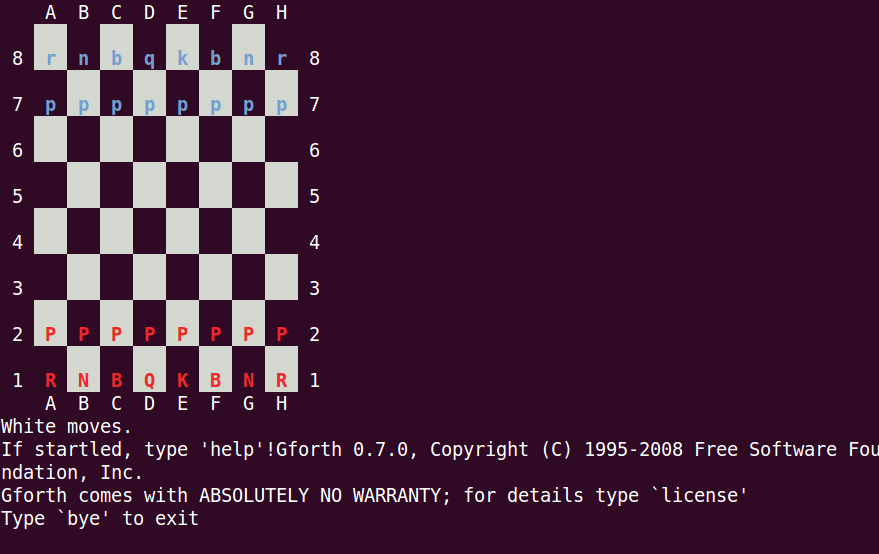
\includegraphics[scale=0.4]{graphics/brainless_before.png}
    \caption{State of the game before entering \emph{d2 d3 m}}
    \label{fig:brainless_before_m}
\end{figure}

\begin{figure}[p]
    \centering
    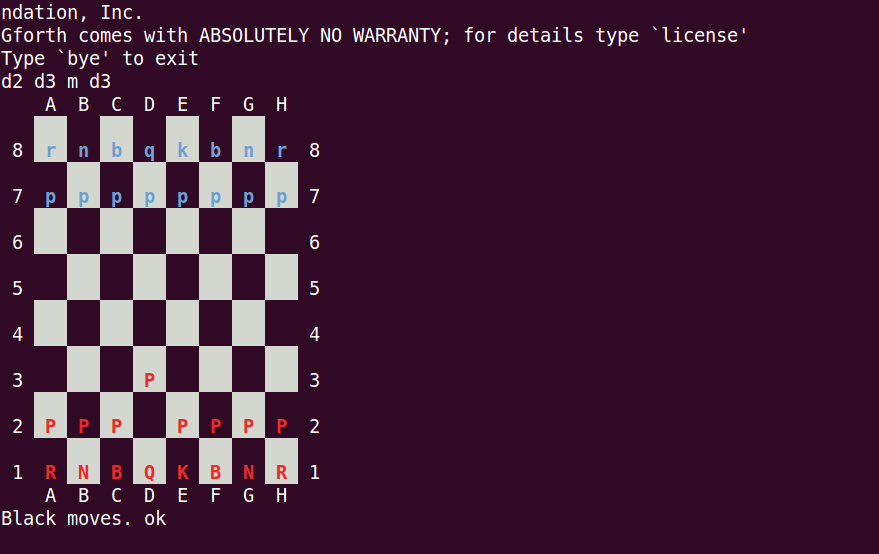
\includegraphics[scale=0.4]{graphics/brainless_after.png}
    \caption{State of the game after entering \emph{d2 d3 m}}
    \label{fig:brainless_after_m}
\end{figure}

\section{The application of the previously presented methods}

\subsection*{Hierarchical edge bundles}

Figure \ref{fig:hierarchic_edge_bundle} shows the trace snapshot mentioned before in a \emph{hierarchic edge bundle}.

\begin{figure}[p]
    \centering
    \begin{tikzpicture}[>=latex,font=\sffamily,semithick,scale=1.75]

	% outer ring
	\draw [thick] (0,0) circle (10);
	\draw [thick] (0,0) circle (9.6);

	% 2. outer ring
    \foreach \angle in {90, 60, ..., -90}
        \draw (\angle:9.6) -- (\angle-180:9.6);
    \draw [thick] (0,0) circle (9.2);

	% 3. outer ring
	% section 90-60
	\foreach \angle in {90, 80, ..., 0}
		\draw (\angle:9.2) -- (\angle-180:0);
	% section 60-30
	%\foreach \angle in {90, 60, ..., -90}
	%	\draw (\angle:9.2) -- (\angle-180:0);
	% section 30-0
	%\foreach \angle in {30, 0}
	%	\draw (\angle:9.2) -- (\angle-180:0);
	\draw [thick,fill=white] (0,0) circle (8.8);

%    \node [circle,thick,fill=white,draw=black,align=center,minimum size=5cm] at (0,0) {};
%    (Head.west);
\end{tikzpicture}
    \caption{Hierarchic edge bundle of Brainless after \emph{d2 d3 m}}
    \label{fig:hierarchic_edge_bundle}
\end{figure}


\subsection*{Information murals and massive sequence view}

Figure \ref{fig:massive_sequence_view} shows the trace snapshot in a \emph{massive sequence view}. It is easy to identify certain steps of the program execution like the drawing part at the end of the trace(interaction withing drawing.fs) and the file writing part(interaction from epd.fs), if one know the words contained in those files. But it also clearly shows the lack of interactivity. Without filtering, zooming, on-demand information on words(references to source code) and of course expressive naming, it still remains hard to map the phases of the trace to behavior. Besides these concerns, the massive sequence view seems to be well applicable to forth program traces.

\begin{figure}[p]
    \centering
    \begin{tikzpicture}[>=latex,font=\sffamily,semithick,scale=2,] % 0.8 fits into latex doc(width only)

\tikzstyle{every node}=[font=\large] %\ŧiny for 0.8 and 20

\def \width { 25 } %20 fits into latex doc(width only)
\pgfmathsetmacro {\dirHeight} { -1 } %
\pgfmathsetmacro {\fileHeight} { 3 }
\pgfmathsetmacro {\wordHeight} { 1 }

\def \interactionHeight { 0.0125 }
\def \wordCount { 663 }

\pgfmathsetmacro {\wordWidth } { \width / \wordCount } % 30 / 663 = 0.045248869


\edef \intRowIdx { 0 }
\newcommand{ \incrementRowIdx } {

	\pgfmathparse { \intRowIdx + 1 } \xdef \intRowIdx { \pgfmathresult }

	%also redefine macro
	\pgfmathsetmacro {\intStartY } { \dirHeight - \fileHeight - \wordHeight - \interactionHeight * \intRowIdx }
	\pgfmathsetmacro {\intEndY } { \intStartY - \interactionHeight }
}

\pgfmathsetmacro {\intStartY } { \dirHeight - \fileHeight - \wordHeight - \interactionHeight * \intRowIdx }
\pgfmathsetmacro {\intEndY } { \intStartY - \interactionHeight }

\newcommand{\drawInteraction}[2]{
	
	\pgfmathparse{#1}
    \pgfmathsetmacro{\from}{\pgfmathresult}
	\pgfmathparse{#2}
    \pgfmathsetmacro{\to}{\pgfmathresult}

	\ifdim \from pt < \to pt

		\def \leftColor{green}
		\def \rightColor{red}	

	\else

		\def \leftColor{red}
		\def \rightColor{green}
		
	\fi

	\fill [left color= \leftColor, right color= \rightColor] 
		({#1}, \intStartY) rectangle ({#2}, \intEndY)-- cycle;

	\incrementRowIdx
}

% file coord offset
\pgfmathsetmacro{\boardFs}				{  									  0 * \wordWidth }
\pgfmathsetmacro{\drawingFs}		{ \boardFs				+ 51 * \wordWidth }
\pgfmathsetmacro{\environFs}			{ \drawingFs		+ 24 * \wordWidth }
\pgfmathsetmacro{\benchmarkFs}	{ \environFs			+ 14 * \wordWidth }
\pgfmathsetmacro{\epdFs}					{ \benchmarkFs	+ 22 * \wordWidth }
\pgfmathsetmacro{\evalFs}				{ \epdFs					+ 25 * \wordWidth }
\pgfmathsetmacro{\flyevalFs}			{ \evalFs					+ 26 * \wordWidth }
\pgfmathsetmacro{\hashFs}				{ \flyevalFs			+ 19 * \wordWidth }
\pgfmathsetmacro{\historyFs}			{ \hashFs				+ 17 * \wordWidth }
\pgfmathsetmacro{\killerFs}				{ \historyFs			+   6 * \wordWidth }
\pgfmathsetmacro{\moveconvFs}		{ \killerFs				+ 43 * \wordWidth }
\pgfmathsetmacro{\movegenFs}		{ \moveconvFs		+ 21 * \wordWidth }
\pgfmathsetmacro{\movesFs}			{ \movegenFs		+ 63 * \wordWidth }
\pgfmathsetmacro{\nullFs}					{ \movesFs			+ 90 * \wordWidth }
\pgfmathsetmacro{\optionsFs}			{ \nullFs					+   5 * \wordWidth }
\pgfmathsetmacro{\profilerFs}			{ \optionsFs			+   0 * \wordWidth }
\pgfmathsetmacro{\quiescenceFs}	{ \profilerFs			+ 13 * \wordWidth }
\pgfmathsetmacro{\repeatFs}			{ \quiescenceFs	+   7 * \wordWidth }
\pgfmathsetmacro{\searchdefsFs}	{ \repeatFs			+   4 * \wordWidth }
\pgfmathsetmacro{\searchFs}			{ \searchdefsFs	+   4 * \wordWidth }
\pgfmathsetmacro{\sglmovesFs}		{ \searchFs			+ 36 * \wordWidth }
\pgfmathsetmacro{\sortingFs}			{ \sglmovesFs		+ 14 * \wordWidth }
\pgfmathsetmacro{\stringFs}				{ \sortingFs			+   6 * \wordWidth }
\pgfmathsetmacro{\testsFs}				{ \stringFs				+ 18 * \wordWidth }
\pgfmathsetmacro{\threatsFs}			{ \testsFs				+ 11 * \wordWidth }
\pgfmathsetmacro{\tmovegenFs}		{ \threatsFs			+ 35 * \wordWidth }
\pgfmathsetmacro{\ttableFs}				{ \tmovegenFs		+ 27 * \wordWidth }
\pgfmathsetmacro{\tuiFs}					{ \ttableFs				+ 14 * \wordWidth }
\pgfmathsetmacro{\utilsFs}				{ \tuiFs					+ 29 * \wordWidth }
\pgfmathsetmacro{\brainlessFs}		{ \utilsFs				+ 15 * \wordWidth }

% word coord offset to the middle of the word section
\newcommand{ \wordOffset }[1] {
	(#1 * \wordWidth - \wordWidth / 2)
}

% word section coords; the index starts at 0
\pgfmathsetmacro{\addMove } 															{ \movesFs + \wordOffset{28} }
\pgfmathsetmacro{\appendMoves } 												{ \movegenFs + \wordOffset{43} }
\pgfmathsetmacro{\appendMoveToSan } 										{ \moveconvFs + \wordOffset{17} }
\pgfmathsetmacro{\bishopMoves } 													{ \movegenFs + \wordOffset{19} }
\pgfmathsetmacro{\bishopThreatensThroughQ } 						{ \threatsFs + \wordOffset{30} }
\pgfmathsetmacro{\bishopThreatsDeltaEval } 								{ \flyevalFs + \wordOffset{2} }
\pgfmathsetmacro{\bishopXyQ } 														{ \boardFs + \wordOffset{11} }
\pgfmathsetmacro{\blackFieldAttr } 												{ \drawingFs + \wordOffset{12} }
\pgfmathsetmacro{\blackPiece } 														{ \boardFs + \wordOffset{29} }
\pgfmathsetmacro{\blackPieceAttr } 												{ \drawingFs + \wordOffset{15} }
\pgfmathsetmacro{\DBoard } 															{ \drawingFs + \wordOffset{32} }
\pgfmathsetmacro{\DBoardLine } 													{ \drawingFs + \wordOffset{30} }
\pgfmathsetmacro{\captureMoveQ } 												{ \movesFs + \wordOffset{33} }
\pgfmathsetmacro{\castleFar } 															{ \movegenFs + \wordOffset{16} }
\pgfmathsetmacro{\castleMoveQ } 													{ \movesFs + \wordOffset{34} }
\pgfmathsetmacro{\castleNear } 														{ \movegenFs + \wordOffset{15} }
\pgfmathsetmacro{\HCharacters } 													{ \stringFs + \wordOffset{6} }
\pgfmathsetmacro{\checkQ } 															{ \threatsFs + \wordOffset{16} }
\pgfmathsetmacro{\currChar } 															{ \stringFs + \wordOffset{11} }
\pgfmathsetmacro{\deltaEval } 															{ \flyevalFs + \wordOffset{6} }
\pgfmathsetmacro{\toDeltaXy } 														{ \boardFs + \wordOffset{10} }
\pgfmathsetmacro{\deltaXyToDirection } 										{ \boardFs + \wordOffset{15} }
\pgfmathsetmacro{\QDirection } 														{ \boardFs + \wordOffset{40} }
\pgfmathsetmacro{\displayMove } 													{ \moveconvFs + \wordOffset{21} }
\pgfmathsetmacro{\doMove } 															{ \movesFs + \wordOffset{87} }
\pgfmathsetmacro{\doMoveUndoInfo } 											{ \movesFs + \wordOffset{86} }
\pgfmathsetmacro{\BdoNormalMoveB } 										{ \movesFs + \wordOffset{63} }
\pgfmathsetmacro{\doNormalMove } 												{ \movesFs + \wordOffset{64} }
\pgfmathsetmacro{\emptyQ } 															{ \boardFs + \wordOffset{33} }
\pgfmathsetmacro{\QEpdAppendToFile } 										{ \epdFs + \wordOffset{26} }
\pgfmathsetmacro{\epdAppendToFile } 											{ \epdFs + \wordOffset{24} }
\pgfmathsetmacro{\epdCloseFile } 													{ \epdFs + \wordOffset{18} }
\pgfmathsetmacro{\epdWriteBoard } 												{ \epdFs + \wordOffset{2} }
\pgfmathsetmacro{\epdWriteBoardLine } 										{ \epdFs + \wordOffset{1} }
\pgfmathsetmacro{\epdWriteCastle } 												{ \epdFs + \wordOffset{4} }
\pgfmathsetmacro{\epdWriteEp } 													{ \epdFs + \wordOffset{5} }
\pgfmathsetmacro{\epdWriteParty } 												{ \epdFs + \wordOffset{3} }
\pgfmathsetmacro{\epdWriteToFile } 												{ \epdFs + \wordOffset{23} }
\pgfmathsetmacro{\evalKnightThreats } 										{ \evalFs + \wordOffset{4} }
\pgfmathsetmacro{\evalPawnThreats } 											{ \evalFs + \wordOffset{3} }
\pgfmathsetmacro{\evalPut } 															{ \flyevalFs + \wordOffset{7} }
\pgfmathsetmacro{\evalRemove } 													{ \flyevalFs + \wordOffset{8} }
\pgfmathsetmacro{\evalStraightThreats } 										{ \evalFs + \wordOffset{2} }
\pgfmathsetmacro{\evalThreat } 														{ \evalFs + \wordOffset{1} }
\pgfmathsetmacro{\fieldAttr } 															{ \drawingFs + \wordOffset{13} }
\pgfmathsetmacro{\DFieldSlice } 														{ \drawingFs + \wordOffset{28} }
\pgfmathsetmacro{\fieldSpaces } 														{ \drawingFs + \wordOffset{17} }
\pgfmathsetmacro{\fileExistsQ } 														{ \utilsFs + \wordOffset{8} }
\pgfmathsetmacro{\QFindMove } 													{ \tuiFs + \wordOffset{18} }
\pgfmathsetmacro{\findMove } 														{ \movesFs + \wordOffset{39} }
\pgfmathsetmacro{\flyEvalMoves } 													{ \flyevalFs + \wordOffset{18} }
\pgfmathsetmacro{\flyEvalNormalMove } 										{ \flyevalFs + \wordOffset{11} }
\pgfmathsetmacro{\forgetMoves } 													{ \movesFs + \wordOffset{38} }
\pgfmathsetmacro{\forgetPosition } 												{ \repeatFs + \wordOffset{3} }
\pgfmathsetmacro{\BgenerateMovesB } 										{ \movegenFs + \wordOffset{42} }
\pgfmathsetmacro{\generateMoves } 												{ \movegenFs + \wordOffset{46} }
\pgfmathsetmacro{\BgenerateMovesFromB } 								{ \movegenFs + \wordOffset{39} }
\pgfmathsetmacro{\BgenerateMoveToB } 										{ \movegenFs + \wordOffset{38} }
\pgfmathsetmacro{\BgenerateMoveToNocheckB } 					{ \movegenFs + \wordOffset{36} }
\pgfmathsetmacro{\getMove } 															{ \movesFs + \wordOffset{23} }
\pgfmathsetmacro{\getMoveClass } 												{ \movesFs + \wordOffset{30} }
\pgfmathsetmacro{\getMoveSquares } 											{ \movesFs + \wordOffset{31} }
\pgfmathsetmacro{\getOrig } 															{ \movesFs + \wordOffset{26} }
\pgfmathsetmacro{\getPieceMasked } 											{ \boardFs + \wordOffset{43} }
\pgfmathsetmacro{\getTarget } 														{ \movesFs + \wordOffset{29} }
\pgfmathsetmacro{\hashFarMovedPawn } 									{ \hashFs + \wordOffset{34} }
\pgfmathsetmacro{\hashPiece } 														{ \hashFs + \wordOffset{31} }
\pgfmathsetmacro{\hashSquare } 													{ \hashFs + \wordOffset{32} }
\pgfmathsetmacro{\Dhborder } 														{ \drawingFs + \wordOffset{31} }
\pgfmathsetmacro{\histRecord } 														{ \historyFs + \wordOffset{2} }
\pgfmathsetmacro{\QInString } 														{ \stringFs + \wordOffset{10} }
\pgfmathsetmacro{\inStringQ } 														{ \stringFs + \wordOffset{9} }
\pgfmathsetmacro{\isString } 															{ \stringFs + \wordOffset{4} }
\pgfmathsetmacro{\QKingEval } 														{ \evalFs + \wordOffset{15} }
\pgfmathsetmacro{\kingMove } 														{ \movegenFs + \wordOffset{12} }
\pgfmathsetmacro{\kingMoves } 														{ \movegenFs + \wordOffset{22} }
\pgfmathsetmacro{\kingSquare } 														{ \boardFs + \wordOffset{29} }
\pgfmathsetmacro{\knightEval } 														{ \evalFs + \wordOffset{21} }
\pgfmathsetmacro{\knightMoves } 													{ \movegenFs + \wordOffset{18} }
\pgfmathsetmacro{\look } 																	{ \tuiFs + \wordOffset{2} }
\pgfmathsetmacro{\m } 																		{ \tuiFs + \wordOffset{20} }
\pgfmathsetmacro{\mightCauseCheckQ } 										{ \threatsFs + \wordOffset{34} }
\pgfmathsetmacro{\moveC } 																{ \movesFs + \wordOffset{22} }
\pgfmathsetmacro{\moveS } 																{ \movesFs + \wordOffset{21} }
\pgfmathsetmacro{\moveF } 																{ \movesFs + \wordOffset{20} }
\pgfmathsetmacro{\moved } 																{ \boardFs + \wordOffset{26} }
\pgfmathsetmacro{\moves } 																{ \movesFs + \wordOffset{19} }
\pgfmathsetmacro{\moveToSan } 														{ \moveconvFs + \wordOffset{18} }
\pgfmathsetmacro{\movesExistQ } 													{ \movegenFs + \wordOffset{63} }
\pgfmathsetmacro{\moveSquares } 													{ \movesFs + \wordOffset{14} }
\pgfmathsetmacro{\moveToString } 												{ \moveconvFs + \wordOffset{20} }
\pgfmathsetmacro{\BmoveToExistsQB } 										{ \movegenFs + \wordOffset{62} }
\pgfmathsetmacro{\BmoveToExistsQNocheckB } 						{ \movegenFs + \wordOffset{60} }
\pgfmathsetmacro{\myPieceQ } 														{ \boardFs + \wordOffset{37} }
\pgfmathsetmacro{\newMoves } 														{ \movesFs + \wordOffset{37} }
\pgfmathsetmacro{\newString } 														{ \stringFs + \wordOffset{2} }
\pgfmathsetmacro{\nextChar } 															{ \stringFs + \wordOffset{7} }
\pgfmathsetmacro{\noAttr } 																{ \drawingFs + \wordOffset{10} }
\pgfmathsetmacro{\opponentQ } 													{ \boardFs + \wordOffset{35} }
\pgfmathsetmacro{\opponentBishopQ } 										{ \threatsFs + \wordOffset{4} }
\pgfmathsetmacro{\opponentKingSquare } 									{ \boardFs + \wordOffset{4} }
\pgfmathsetmacro{\opponentKnightQ } 										{ \threatsFs + \wordOffset{2} }
\pgfmathsetmacro{\opponentMoveOrig } 										{ \movesFs + \wordOffset{12} }
\pgfmathsetmacro{\opponentMoveTarget } 									{ \movesFs + \wordOffset{9} }
\pgfmathsetmacro{\opponentPawnQ } 											{ \threatsFs + \wordOffset{1} }
\pgfmathsetmacro{\opponentPieces } 											{ \boardFs + \wordOffset{47} }
\pgfmathsetmacro{\opponentRookQ } 											{ \threatsFs + \wordOffset{5} }
\pgfmathsetmacro{\otherParty } 														{ \boardFs + \wordOffset{17} }
\pgfmathsetmacro{\DParty } 																{ \tuiFs + \wordOffset{1} }
\pgfmathsetmacro{\pawnQ } 																{ \boardFs + \wordOffset{39} }
\pgfmathsetmacro{\pawnDeltaEval } 												{ \flyevalFs + \wordOffset{4} }
\pgfmathsetmacro{\QPawnEval } 														{ \evalFs + \wordOffset{14} }
\pgfmathsetmacro{\pawnFarMove } 												{ \movegenFs + \wordOffset{4} }
\pgfmathsetmacro{\pawnMoves } 													{ \movegenFs + \wordOffset{17} }
\pgfmathsetmacro{\pawnNormalMove } 										{ \movegenFs + \wordOffset{7} }
\pgfmathsetmacro{\pawnRowEval } 												{ \evalFs + \wordOffset{13} }
\pgfmathsetmacro{\pawnStrikeMove } 											{ \movegenFs + \wordOffset{8} }
\pgfmathsetmacro{\pawnTransQ } 													{ \boardFs + \wordOffset{41} }
\pgfmathsetmacro{\DPiece } 																{ \drawingFs + \wordOffset{18} }
\pgfmathsetmacro{\BDPieceB } 														{ \drawingFs + \wordOffset{9} }
\pgfmathsetmacro{\pieceQ } 																{ \boardFs + \wordOffset{36} }
\pgfmathsetmacro{\pieceToAscii } 													{ \drawingFs + \wordOffset{6} }
\pgfmathsetmacro{\pieceAttr } 															{ \drawingFs + \wordOffset{16} }
\pgfmathsetmacro{\pieceToChar } 													{ \boardFs + \wordOffset{50} }
\pgfmathsetmacro{\pieceDeltaEval } 												{ \flyevalFs + \wordOffset{5} }
\pgfmathsetmacro{\pieceToString } 												{ \drawingFs + \wordOffset{8} }
\pgfmathsetmacro{\pieceThreateningThrough } 							{ \threatsFs + \wordOffset{29} }
\pgfmathsetmacro{\positionToEpd } 												{ \epdFs + \wordOffset{6} }
\pgfmathsetmacro{\previousString } 												{ \stringFs + \wordOffset{3} }
\pgfmathsetmacro{\putPiece } 															{ \boardFs + \wordOffset{45} }
\pgfmathsetmacro{\queenlikeThreatensThroughQ } 					{ \threatsFs + \wordOffset{32} }
\pgfmathsetmacro{\queenMoves } 													{ \movegenFs + \wordOffset{21} }
\pgfmathsetmacro{\rememberPosition } 										{ \repeatFs + \wordOffset{2} }
\pgfmathsetmacro{\removePiece } 													{ \boardFs + \wordOffset{42} }
\pgfmathsetmacro{\rookMoves } 														{ \movegenFs + \wordOffset{20} }
\pgfmathsetmacro{\rookThreatensThroughQ } 							{ \threatsFs + \wordOffset{31} }
\pgfmathsetmacro{\rookThreatsDeltaEval } 									{ \flyevalFs + \wordOffset{1} }
\pgfmathsetmacro{\rookXyQ } 															{ \boardFs + \wordOffset{12} }
\pgfmathsetmacro{\selectMovingPiece } 										{ \movegenFs + \wordOffset{35} }
\pgfmathsetmacro{\setEval } 																{ \movesFs + \wordOffset{27} }
\pgfmathsetmacro{\setThisPawnAKing } 										{ \evalFs + \wordOffset{12} }
\pgfmathsetmacro{\toSquare } 															{ \boardFs + \wordOffset{6} }
\pgfmathsetmacro{\squareWhiteQ } 												{ \boardFs + \wordOffset{52} }
\pgfmathsetmacro{\straightMoves } 												{ \movegenFs + \wordOffset{11} }
\pgfmathsetmacro{\strikeEpMove } 												{ \movegenFs + \wordOffset{5} }
\pgfmathsetmacro{\strikeQMove } 													{ \movegenFs + \wordOffset{3} }
\pgfmathsetmacro{\takePiece } 														{ \boardFs + \wordOffset{44} }
\pgfmathsetmacro{\threatenedByBishopQ } 								{ \threatsFs + \wordOffset{8} }
\pgfmathsetmacro{\threatenedByKingQ } 									{ \threatsFs + \wordOffset{10} }
\pgfmathsetmacro{\threatenedByKnightQ } 								{ \threatsFs + \wordOffset{7} }
\pgfmathsetmacro{\threatenedByOpponentQ } 							{ \threatsFs + \wordOffset{13} }
\pgfmathsetmacro{\threatenedByPawnQ } 									{ \threatsFs + \wordOffset{6} }
\pgfmathsetmacro{\threatenedByPieceQ } 									{ \threatsFs + \wordOffset{11} }
\pgfmathsetmacro{\threatenedByRookQ } 									{ \threatsFs + \wordOffset{9} }
\pgfmathsetmacro{\threatensQ } 														{ \threatsFs + \wordOffset{28} }
\pgfmathsetmacro{\threatsDeltaEval } 											{ \flyevalFs + \wordOffset{3} }
\pgfmathsetmacro{\toMoveSquares } 												{ \movesFs + \wordOffset{16} }
\pgfmathsetmacro{\undoInfo } 															{ \movesFs + \wordOffset{62} }
\pgfmathsetmacro{\undoMove } 														{ \movesFs + \wordOffset{88} }
\pgfmathsetmacro{\undoNormalMove } 										{ \movesFs + \wordOffset{53} }
\pgfmathsetmacro{\unmoved } 															{ \boardFs + \wordOffset{25} }
\pgfmathsetmacro{\unmovedQ } 														{ \boardFs + \wordOffset{38} }
\pgfmathsetmacro{\updateCurrCheckQ } 										{ \movesFs + \wordOffset{85} }
\pgfmathsetmacro{\updateHash } 													{ \hashFs + \wordOffset{30} }
\pgfmathsetmacro{\QValidMove } 													{ \tuiFs + \wordOffset{19} }
\pgfmathsetmacro{\DVborderSlice } 												{ \drawingFs + \wordOffset{29} }
\pgfmathsetmacro{\whiteFieldAttr } 												{ \drawingFs + \wordOffset{11} }
\pgfmathsetmacro{\whitePawnThreatensQ } 								{ \threatsFs + \wordOffset{18} }
\pgfmathsetmacro{\whitePiece } 														{ \boardFs + \wordOffset{28} }
\pgfmathsetmacro{\whitePieceAttr } 												{ \drawingFs + \wordOffset{14} }
\pgfmathsetmacro{\writeChar } 														{ \stringFs + \wordOffset{12} }
\pgfmathsetmacro{\writeCheckState } 											{ \moveconvFs + \wordOffset{1} }
\pgfmathsetmacro{\writePawnMoveSan } 										{ \moveconvFs + \wordOffset{14} }
\pgfmathsetmacro{\writePawnTrans } 											{ \moveconvFs + \wordOffset{2} }
\pgfmathsetmacro{\writeSquare } 													{ \stringFs + \wordOffset{17} }
\pgfmathsetmacro{\writeSquareFile } 											{ \stringFs + \wordOffset{15} }
\pgfmathsetmacro{\writeSquareRank } 											{ \stringFs + \wordOffset{16} }
\pgfmathsetmacro{\writeString } 														{ \stringFs + \wordOffset{14} }
\pgfmathsetmacro{\toXy } 																	{ \boardFs + \wordOffset{39} }
\pgfmathsetmacro{\xyBoardF }	 														{ \boardFs + \wordOffset{41} }

\def \fileYMax {\dirHeight - \fileHeight}
\def \fileYMin {\dirHeight}
% the xcoord of middle of the file section limited by the factors arg1 and arg2
\newcommand{ \fileTextX }[2] {
	( \wordWidth * (#1 + (#2 - #1) / 2) )
}
\pgfmathsetmacro{\fileTextY } { \fileYMin + (\fileYMax - \fileYMin) / 2 }



% dir ------- y 0 to -1
\draw (0,0) rectangle (\width, \dirHeight);
\node [font=\large] at (\width / 2, \dirHeight / 2) {brainless-0.1.2}; 

% files ------- y -1 to -2.5

\draw (\wordWidth *      0,\fileYMin) rectangle (\wordWidth *   51,\fileYMax); %board.fs 51 sections
\node [rotate=90] at ({\fileTextX{0}{51}}, \fileTextY) {board.fs}; 
\draw (\wordWidth *   51,\fileYMin) rectangle (\wordWidth *   75,\fileYMax); %drawing.fs 24 sections
\node [rotate=90] at ({\fileTextX{51}{75}} , \fileTextY) {drawing.fs}; 
\draw (\wordWidth *   75,\fileYMin) rectangle (\wordWidth *   89,\fileYMax); %environ.fs 14 sections
\node [rotate=90] at ({\fileTextX{75}{89}} , \fileTextY) {environ.fs}; 
\draw (\wordWidth *   89,\fileYMin) rectangle (\wordWidth * 111,\fileYMax); %benchmark.fs 22 sections
\node [rotate=90] at ({\fileTextX{89}{111}} , \fileTextY) {benchmark.fs}; 
\draw (\wordWidth * 111,\fileYMin) rectangle (\wordWidth * 136,\fileYMax); %epd.fs 25 sections
\node [rotate=90] at ({\fileTextX{111}{136}} , \fileTextY) {epd.fs}; 
\draw (\wordWidth * 136,\fileYMin) rectangle (\wordWidth * 162,\fileYMax); %eval.fs 26 sections
\node [rotate=90] at ({\fileTextX{136}{162}} , \fileTextY) {eval.fs}; 
\draw (\wordWidth * 162,\fileYMin) rectangle (\wordWidth * 181,\fileYMax); %flyeval.fs 19 sections
\node [rotate=90] at ({\fileTextX{162}{181}} , \fileTextY) {flyeval.fs}; 
\draw (\wordWidth * 181,\fileYMin) rectangle (\wordWidth * 198,\fileYMax); %hash.fs 17 sections
\node [rotate=90] at ({\fileTextX{181}{198}} , \fileTextY) {hash.fs}; 
\draw (\wordWidth * 198,\fileYMin) rectangle (\wordWidth * 204,\fileYMax); %history.fs 6 sections
\node [rotate=90] at ({\fileTextX{198}{204}} , \fileTextY) {history.fs}; 
\draw (\wordWidth * 204,\fileYMin) rectangle (\wordWidth * 247,\fileYMax); %killer.fs 43 sections
\node [rotate=90] at ({\fileTextX{204}{247}} , \fileTextY) {killer.fs}; 
\draw (\wordWidth * 247,\fileYMin) rectangle (\wordWidth * 268,\fileYMax); %moveconv.fs 21 sections
\node [rotate=90] at ({\fileTextX{247}{268}} , \fileTextY) {moveconv.fs}; 
\draw (\wordWidth * 268,\fileYMin) rectangle (\wordWidth * 331,\fileYMax); %movegen.fs 63 sections
\node [rotate=90] at ({\fileTextX{268}{331}} , \fileTextY) {movegen.fs}; 
\draw (\wordWidth * 331,\fileYMin) rectangle (\wordWidth * 421,\fileYMax); %moves.fs 90 sections
\node [] at ({\fileTextX{331}{421}} , \fileTextY) {moves.fs}; 
\draw (\wordWidth * 421,\fileYMin) rectangle (\wordWidth * 426,\fileYMax); %null.fs 5 sections
\node [rotate=90] at ({\fileTextX{421}{426}} , \fileTextY) {null.fs}; 
%\draw (\wordWidth * 426,\fileYMin) rectangle (\wordWidth * 426,\fileYMax); %options.fs 0 sections
%\node [] at ({\fileTextX{426}{426}} , \fileTextY) {options.fs}; 
\draw (\wordWidth * 426,\fileYMin) rectangle (\wordWidth * 439,\fileYMax); %profiler.fs 13 sections
\node [rotate=90] at ({\fileTextX{426}{439}} , \fileTextY) {profiler.fs}; 
\draw (\wordWidth * 439,\fileYMin) rectangle (\wordWidth * 446,\fileYMax); %quiescence.fs 7 sections
\node [rotate=90] at ({\fileTextX{439}{446}} , \fileTextY) {quiescence.fs}; 
\draw (\wordWidth * 446,\fileYMin) rectangle (\wordWidth * 450,\fileYMax); %repeat.fs 4 sections
\node [rotate=90] at ({\fileTextX{446}{450}} , \fileTextY) {repeat.fs}; 
\draw (\wordWidth * 450,\fileYMin) rectangle (\wordWidth * 454,\fileYMax); %searchdefs.fs 4 sections
\node [rotate=90] at ({\fileTextX{450}{454}} , \fileTextY) {searchdefs.fs}; 
\draw (\wordWidth * 454,\fileYMin) rectangle (\wordWidth * 490,\fileYMax); %search.fs 36 sections
\node [rotate=90] at ({\fileTextX{454}{490}} , \fileTextY) {search.fs}; 
\draw (\wordWidth * 490,\fileYMin) rectangle (\wordWidth * 504,\fileYMax); %sglmoves.fs 14 sections
\node [rotate=90] at ({\fileTextX{490}{504}} , \fileTextY) {sglmoves.fs}; 
\draw (\wordWidth * 504,\fileYMin) rectangle (\wordWidth * 510,\fileYMax); %sorting.fs 6 sections
\node [rotate=90] at ({\fileTextX{504}{510}} , \fileTextY) {sorting.fs}; 
\draw (\wordWidth * 510,\fileYMin) rectangle (\wordWidth * 528,\fileYMax); %string.fs 18 sections
\node [rotate=90] at ({\fileTextX{510}{528}} , \fileTextY) {string.fs}; 
\draw (\wordWidth * 528,\fileYMin) rectangle (\wordWidth * 539,\fileYMax); %tests.fs 11 sections
\node [rotate=90] at ({\fileTextX{528}{539}} , \fileTextY) {tests.fs}; 
\draw (\wordWidth * 539,\fileYMin) rectangle (\wordWidth * 574,\fileYMax); %threats.fs 35 sections
\node [rotate=90] at ({\fileTextX{539}{574}} , \fileTextY) {threats.fs}; 
\draw (\wordWidth * 574,\fileYMin) rectangle (\wordWidth * 601,\fileYMax); %tmovegen.fs 27 sections
\node [rotate=90] at ({\fileTextX{574}{601}} , \fileTextY) {tmovegen.fs}; 
\draw (\wordWidth * 601,\fileYMin) rectangle (\wordWidth * 615,\fileYMax); %ttable.fs 14 sections
\node [rotate=90] at ({\fileTextX{601}{615}} , \fileTextY) {ttable.fs}; 
\draw (\wordWidth * 615,\fileYMin) rectangle (\wordWidth * 644,\fileYMax); %tui.fs 29 sections
\node [rotate=90] at ({\fileTextX{615}{644}} , \fileTextY) {tui.fs}; 
\draw (\wordWidth * 644,\fileYMin) rectangle (\wordWidth * 659,\fileYMax); %utils.fs 15 sections
\node [rotate=90] at ({\fileTextX{644}{659}} , \fileTextY) {utils.fs}; 
\draw (\wordWidth * 659,\fileYMin) rectangle (\wordWidth * 663,\fileYMax); %brainless.fs 4 sections
\node [rotate=90] at ({\fileTextX{659}{663}} , \fileTextY) {brainless.fs}; 

% words ------- y -2 to -3
\foreach \x in {1,...,\wordCount}
	\draw (\x * \wordWidth - \wordWidth,\fileYMax) rectangle (\x * \wordWidth,\fileYMax - 1);


% interactions ------- y -3
\drawInteraction{\m}{\QValidMove}
\drawInteraction{\QValidMove}{\generateMoves}
\drawInteraction{\generateMoves}{\newMoves}
\drawInteraction{\generateMoves}{\appendMoves}
\drawInteraction{\appendMoves}{\BgenerateMovesB}
\drawInteraction{\BgenerateMovesB}{\myPieceQ}
\drawInteraction{\BgenerateMovesB}{\myPieceQ}
\drawInteraction{\BgenerateMovesB}{\BgenerateMovesFromB}
\drawInteraction{\BgenerateMovesFromB}{\selectMovingPiece}
\drawInteraction{\BgenerateMovesFromB}{\rookMoves}
\drawInteraction{\rookMoves}{\straightMoves}
\drawInteraction{\rookMoves}{\straightMoves}
\drawInteraction{\rookMoves}{\straightMoves}
\drawInteraction{\rookMoves}{\straightMoves}
\drawInteraction{\BgenerateMovesB}{\myPieceQ}
\drawInteraction{\BgenerateMovesB}{\BgenerateMovesFromB}
\drawInteraction{\BgenerateMovesFromB}{\selectMovingPiece}
\drawInteraction{\BgenerateMovesFromB}{\knightMoves}
\drawInteraction{\knightMoves}{\strikeQMove}
\drawInteraction{\strikeQMove}{\BgenerateMoveToB}
\drawInteraction{\BgenerateMoveToB}{\BgenerateMoveToNocheckB}
\drawInteraction{\BgenerateMoveToNocheckB}{\mightCauseCheckQ}
\drawInteraction{\mightCauseCheckQ}{\kingSquare}
\drawInteraction{\mightCauseCheckQ}{\queenlikeThreatensThroughQ}
\drawInteraction{\queenlikeThreatensThroughQ}{\toDeltaXy}
\drawInteraction{\queenlikeThreatensThroughQ}{\bishopXyQ}
\drawInteraction{\queenlikeThreatensThroughQ}{\rookXyQ}
\drawInteraction{\queenlikeThreatensThroughQ}{\deltaXyToDirection}
\drawInteraction{\queenlikeThreatensThroughQ}{\rookThreatensThroughQ}
\drawInteraction{\rookThreatensThroughQ}{\pieceThreateningThrough}
\drawInteraction{\BgenerateMoveToNocheckB}{\addMove}
\drawInteraction{\addMove}{\moveC}
\drawInteraction{\moveC}{\moveS}
\drawInteraction{\knightMoves}{\strikeQMove}
\drawInteraction{\knightMoves}{\strikeQMove}
\drawInteraction{\strikeQMove}{\BgenerateMoveToB}
\drawInteraction{\BgenerateMoveToB}{\BgenerateMoveToNocheckB}
\drawInteraction{\BgenerateMoveToNocheckB}{\mightCauseCheckQ}
\drawInteraction{\mightCauseCheckQ}{\kingSquare}
\drawInteraction{\kingSquare}{\queenlikeThreatensThroughQ}
\drawInteraction{\queenlikeThreatensThroughQ}{\toDeltaXy}
\drawInteraction{\queenlikeThreatensThroughQ}{\bishopXyQ}
\drawInteraction{\queenlikeThreatensThroughQ}{\rookXyQ}
\drawInteraction{\queenlikeThreatensThroughQ}{\deltaXyToDirection}
\drawInteraction{\queenlikeThreatensThroughQ}{\rookThreatensThroughQ}
\drawInteraction{\rookThreatensThroughQ}{\pieceThreateningThrough}
\drawInteraction{\BgenerateMoveToNocheckB}{\addMove}
\drawInteraction{\addMove}{\moveC}
\drawInteraction{\moveC}{\moveS}
\drawInteraction{\knightMoves}{\strikeQMove}
\drawInteraction{\knightMoves}{\strikeQMove}
\drawInteraction{\knightMoves}{\strikeQMove}
\drawInteraction{\knightMoves}{\strikeQMove}
\drawInteraction{\knightMoves}{\strikeQMove}
\drawInteraction{\BgenerateMovesB}{\myPieceQ}
\drawInteraction{\BgenerateMovesB}{\BgenerateMovesFromB}
\drawInteraction{\BgenerateMovesFromB}{\selectMovingPiece}
\drawInteraction{\BgenerateMovesFromB}{\bishopMoves}
\drawInteraction{\bishopMoves}{\straightMoves}
\drawInteraction{\bishopMoves}{\straightMoves}
\drawInteraction{\bishopMoves}{\straightMoves}
\drawInteraction{\bishopMoves}{\straightMoves}
\drawInteraction{\BgenerateMovesB}{\myPieceQ}
\drawInteraction{\BgenerateMovesB}{\BgenerateMovesFromB}
\drawInteraction{\BgenerateMovesFromB}{\selectMovingPiece}
\drawInteraction{\BgenerateMovesFromB}{\queenMoves}
\drawInteraction{\queenMoves}{\bishopMoves}
\drawInteraction{\bishopMoves}{\straightMoves}
\drawInteraction{\bishopMoves}{\straightMoves}
\drawInteraction{\bishopMoves}{\straightMoves}
\drawInteraction{\bishopMoves}{\straightMoves}
\drawInteraction{\queenMoves}{\rookMoves}
\drawInteraction{\bishopMoves}{\straightMoves}
\drawInteraction{\bishopMoves}{\straightMoves}
\drawInteraction{\bishopMoves}{\straightMoves}
\drawInteraction{\bishopMoves}{\straightMoves}
\drawInteraction{\BgenerateMovesB}{\myPieceQ}
\drawInteraction{\BgenerateMovesB}{\BgenerateMovesFromB}
\drawInteraction{\BgenerateMovesFromB}{\selectMovingPiece}
\drawInteraction{\BgenerateMovesFromB}{\kingMoves}
\drawInteraction{\kingMoves}{\kingMove}
\drawInteraction{\kingMoves}{\kingMove}
\drawInteraction{\kingMoves}{\kingMove}
\drawInteraction{\kingMoves}{\kingMove}
\drawInteraction{\kingMoves}{\kingMove}
\drawInteraction{\kingMoves}{\kingMove}
\drawInteraction{\kingMoves}{\kingMove}
\drawInteraction{\kingMoves}{\kingMove}
\drawInteraction{\kingMoves}{\castleNear}
\drawInteraction{\castleNear}{\emptyQ}
\drawInteraction{\castleNear}{\emptyQ}
\drawInteraction{\castleNear}{\unmovedQ}
\drawInteraction{\kingMoves}{\castleFar}
\drawInteraction{\castleFar}{\emptyQ}
\drawInteraction{\castleFar}{\emptyQ}
\drawInteraction{\castleFar}{\emptyQ}
\drawInteraction{\castleFar}{\unmovedQ}
\drawInteraction{\BgenerateMovesB}{\myPieceQ}
\drawInteraction{\BgenerateMovesB}{\BgenerateMovesFromB}
\drawInteraction{\BgenerateMovesFromB}{\selectMovingPiece}
\drawInteraction{\BgenerateMovesFromB}{\bishopMoves}
\drawInteraction{\bishopMoves}{\straightMoves}
\drawInteraction{\bishopMoves}{\straightMoves}
\drawInteraction{\bishopMoves}{\straightMoves}
\drawInteraction{\bishopMoves}{\straightMoves}
\drawInteraction{\BgenerateMovesB}{\myPieceQ}
\drawInteraction{\BgenerateMovesB}{\BgenerateMovesFromB}
\drawInteraction{\BgenerateMovesFromB}{\selectMovingPiece}
\drawInteraction{\BgenerateMovesFromB}{\knightMoves}
\drawInteraction{\knightMoves}{\strikeQMove}
\drawInteraction{\strikeQMove}{\BgenerateMoveToB}
\drawInteraction{\BgenerateMoveToB}{\BgenerateMoveToNocheckB}
\drawInteraction{\BgenerateMoveToNocheckB}{\mightCauseCheckQ}
\drawInteraction{\mightCauseCheckQ}{\kingSquare}
\drawInteraction{\mightCauseCheckQ}{\queenlikeThreatensThroughQ}
\drawInteraction{\queenlikeThreatensThroughQ}{\toDeltaXy}
\drawInteraction{\queenlikeThreatensThroughQ}{\bishopXyQ}
\drawInteraction{\queenlikeThreatensThroughQ}{\rookXyQ}
\drawInteraction{\queenlikeThreatensThroughQ}{\deltaXyToDirection}
\drawInteraction{\queenlikeThreatensThroughQ}{\rookThreatensThroughQ}
\drawInteraction{\rookThreatensThroughQ}{\pieceThreateningThrough}
\drawInteraction{\BgenerateMoveToNocheckB}{\addMove}
\drawInteraction{\addMove}{\moveC}
\drawInteraction{\moveC}{\moveS}
\drawInteraction{\knightMoves}{\strikeQMove}
\drawInteraction{\knightMoves}{\strikeQMove}
\drawInteraction{\strikeQMove}{\BgenerateMoveToB}
\drawInteraction{\BgenerateMoveToB}{\BgenerateMoveToNocheckB}
\drawInteraction{\BgenerateMoveToNocheckB}{\mightCauseCheckQ}
\drawInteraction{\mightCauseCheckQ}{\kingSquare}
\drawInteraction{\kingSquare}{\queenlikeThreatensThroughQ}
\drawInteraction{\queenlikeThreatensThroughQ}{\toDeltaXy}
\drawInteraction{\queenlikeThreatensThroughQ}{\bishopXyQ}
\drawInteraction{\queenlikeThreatensThroughQ}{\rookXyQ}
\drawInteraction{\queenlikeThreatensThroughQ}{\deltaXyToDirection}
\drawInteraction{\queenlikeThreatensThroughQ}{\rookThreatensThroughQ}
\drawInteraction{\rookThreatensThroughQ}{\pieceThreateningThrough}
\drawInteraction{\BgenerateMoveToNocheckB}{\addMove}
\drawInteraction{\addMove}{\moveC}
\drawInteraction{\moveC}{\moveS}
\drawInteraction{\knightMoves}{\strikeQMove}
\drawInteraction{\knightMoves}{\strikeQMove}
\drawInteraction{\knightMoves}{\strikeQMove}
\drawInteraction{\knightMoves}{\strikeQMove}
\drawInteraction{\knightMoves}{\strikeQMove}
\drawInteraction{\BgenerateMovesB}{\myPieceQ}
\drawInteraction{\BgenerateMovesB}{\BgenerateMovesFromB}
\drawInteraction{\BgenerateMovesFromB}{\selectMovingPiece}
\drawInteraction{\BgenerateMovesFromB}{\rookMoves}
\drawInteraction{\rookMoves}{\straightMoves}
\drawInteraction{\rookMoves}{\straightMoves}
\drawInteraction{\rookMoves}{\straightMoves}
\drawInteraction{\rookMoves}{\straightMoves}
\drawInteraction{\BgenerateMovesB}{\myPieceQ}
\drawInteraction{\BgenerateMovesB}{\myPieceQ}
\drawInteraction{\BgenerateMovesB}{\myPieceQ}
\drawInteraction{\BgenerateMovesB}{\BgenerateMovesFromB}
\drawInteraction{\BgenerateMovesFromB}{\selectMovingPiece}
\drawInteraction{\BgenerateMovesFromB}{\pawnMoves}
\drawInteraction{\pawnMoves}{\QDirection}
\drawInteraction{\pawnMoves}{\pawnFarMove}
\drawInteraction{\pawnFarMove}{\emptyQ}
\drawInteraction{\pawnFarMove}{\QDirection}
\drawInteraction{\pawnFarMove}{\emptyQ}
\drawInteraction{\pawnFarMove}{\BgenerateMoveToB}
\drawInteraction{\BgenerateMoveToB}{\BgenerateMoveToNocheckB}
\drawInteraction{\BgenerateMoveToNocheckB}{\mightCauseCheckQ}
\drawInteraction{\mightCauseCheckQ}{\kingSquare}
\drawInteraction{\mightCauseCheckQ}{\queenlikeThreatensThroughQ}
\drawInteraction{\queenlikeThreatensThroughQ}{\toDeltaXy}
\drawInteraction{\queenlikeThreatensThroughQ}{\bishopXyQ}
\drawInteraction{\queenlikeThreatensThroughQ}{\rookXyQ}
\drawInteraction{\BgenerateMoveToNocheckB}{\addMove}
\drawInteraction{\addMove}{\moveC}
\drawInteraction{\moveC}{\moveS}
\drawInteraction{\pawnMoves}{\QDirection}
\drawInteraction{\pawnMoves}{\pawnNormalMove}
\drawInteraction{\pawnNormalMove}{\emptyQ}
\drawInteraction{\pawnNormalMove}{\pawnTransQ}
\drawInteraction{\pawnNormalMove}{\BgenerateMoveToB}
\drawInteraction{\BgenerateMoveToB}{\BgenerateMoveToNocheckB}
\drawInteraction{\BgenerateMoveToNocheckB}{\mightCauseCheckQ}
\drawInteraction{\mightCauseCheckQ}{\kingSquare}
\drawInteraction{\mightCauseCheckQ}{\queenlikeThreatensThroughQ}
\drawInteraction{\queenlikeThreatensThroughQ}{\toDeltaXy}
\drawInteraction{\queenlikeThreatensThroughQ}{\bishopXyQ}
\drawInteraction{\queenlikeThreatensThroughQ}{\rookXyQ}
\drawInteraction{\BgenerateMoveToNocheckB}{\addMove}
\drawInteraction{\addMove}{\moveC}
\drawInteraction{\moveC}{\moveS}
\drawInteraction{\pawnMoves}{\QDirection}
\drawInteraction{\pawnMoves}{\pawnStrikeMove}
\drawInteraction{\pawnStrikeMove}{\opponentQ}
\drawInteraction{\pawnMoves}{\strikeEpMove}
\drawInteraction{\strikeEpMove}{\QDirection}
\drawInteraction{\pawnMoves}{\QDirection}
\drawInteraction{\pawnMoves}{\pawnStrikeMove}
\drawInteraction{\pawnStrikeMove}{\opponentQ}
\drawInteraction{\pawnMoves}{\strikeEpMove}
\drawInteraction{\strikeEpMove}{\QDirection}
\drawInteraction{\BgenerateMovesB}{\myPieceQ}
\drawInteraction{\BgenerateMovesB}{\BgenerateMovesFromB}
\drawInteraction{\BgenerateMovesFromB}{\selectMovingPiece}
\drawInteraction{\BgenerateMovesFromB}{\pawnMoves}
\drawInteraction{\pawnMoves}{\QDirection}
\drawInteraction{\pawnMoves}{\pawnFarMove}
\drawInteraction{\pawnFarMove}{\emptyQ}
\drawInteraction{\pawnFarMove}{\QDirection}
\drawInteraction{\pawnFarMove}{\emptyQ}
\drawInteraction{\pawnFarMove}{\BgenerateMoveToB}
\drawInteraction{\BgenerateMoveToB}{\BgenerateMoveToNocheckB}
\drawInteraction{\BgenerateMoveToNocheckB}{\mightCauseCheckQ}
\drawInteraction{\mightCauseCheckQ}{\kingSquare}
\drawInteraction{\mightCauseCheckQ}{\queenlikeThreatensThroughQ}
\drawInteraction{\queenlikeThreatensThroughQ}{\toDeltaXy}
\drawInteraction{\queenlikeThreatensThroughQ}{\bishopXyQ}
\drawInteraction{\queenlikeThreatensThroughQ}{\rookXyQ}
\drawInteraction{\BgenerateMoveToNocheckB}{\addMove}
\drawInteraction{\addMove}{\moveC}
\drawInteraction{\moveC}{\moveS}
\drawInteraction{\pawnMoves}{\QDirection}
\drawInteraction{\pawnMoves}{\pawnNormalMove}
\drawInteraction{\pawnNormalMove}{\emptyQ}
\drawInteraction{\pawnNormalMove}{\pawnTransQ}
\drawInteraction{\pawnNormalMove}{\BgenerateMoveToB}
\drawInteraction{\BgenerateMoveToB}{\BgenerateMoveToNocheckB}
\drawInteraction{\BgenerateMoveToNocheckB}{\mightCauseCheckQ}
\drawInteraction{\mightCauseCheckQ}{\kingSquare}
\drawInteraction{\mightCauseCheckQ}{\queenlikeThreatensThroughQ}
\drawInteraction{\queenlikeThreatensThroughQ}{\toDeltaXy}
\drawInteraction{\queenlikeThreatensThroughQ}{\bishopXyQ}
\drawInteraction{\queenlikeThreatensThroughQ}{\rookXyQ}
\drawInteraction{\BgenerateMoveToNocheckB}{\addMove}
\drawInteraction{\addMove}{\moveC}
\drawInteraction{\moveC}{\moveS}
\drawInteraction{\pawnMoves}{\QDirection}
\drawInteraction{\pawnMoves}{\pawnStrikeMove}
\drawInteraction{\pawnStrikeMove}{\opponentQ}
\drawInteraction{\pawnMoves}{\strikeEpMove}
\drawInteraction{\strikeEpMove}{\QDirection}
\drawInteraction{\pawnMoves}{\QDirection}
\drawInteraction{\pawnMoves}{\pawnStrikeMove}
\drawInteraction{\pawnStrikeMove}{\opponentQ}
\drawInteraction{\pawnMoves}{\strikeEpMove}
\drawInteraction{\strikeEpMove}{\QDirection}
\drawInteraction{\BgenerateMovesB}{\myPieceQ}
\drawInteraction{\BgenerateMovesB}{\BgenerateMovesFromB}
\drawInteraction{\BgenerateMovesFromB}{\selectMovingPiece}
\drawInteraction{\BgenerateMovesFromB}{\pawnMoves}
\drawInteraction{\pawnMoves}{\QDirection}
\drawInteraction{\pawnMoves}{\pawnFarMove}
\drawInteraction{\pawnFarMove}{\emptyQ}
\drawInteraction{\pawnFarMove}{\QDirection}
\drawInteraction{\pawnFarMove}{\emptyQ}
\drawInteraction{\pawnFarMove}{\BgenerateMoveToB}
\drawInteraction{\BgenerateMoveToB}{\BgenerateMoveToNocheckB}
\drawInteraction{\BgenerateMoveToNocheckB}{\mightCauseCheckQ}
\drawInteraction{\mightCauseCheckQ}{\kingSquare}
\drawInteraction{\mightCauseCheckQ}{\queenlikeThreatensThroughQ}
\drawInteraction{\queenlikeThreatensThroughQ}{\toDeltaXy}
\drawInteraction{\queenlikeThreatensThroughQ}{\bishopXyQ}
\drawInteraction{\queenlikeThreatensThroughQ}{\rookXyQ}
\drawInteraction{\BgenerateMoveToNocheckB}{\addMove}
\drawInteraction{\addMove}{\moveC}
\drawInteraction{\moveC}{\moveS}
\drawInteraction{\pawnMoves}{\QDirection}
\drawInteraction{\pawnMoves}{\pawnNormalMove}
\drawInteraction{\pawnNormalMove}{\emptyQ}
\drawInteraction{\pawnNormalMove}{\pawnTransQ}
\drawInteraction{\pawnNormalMove}{\BgenerateMoveToB}
\drawInteraction{\BgenerateMoveToB}{\BgenerateMoveToNocheckB}
\drawInteraction{\BgenerateMoveToNocheckB}{\mightCauseCheckQ}
\drawInteraction{\mightCauseCheckQ}{\kingSquare}
\drawInteraction{\mightCauseCheckQ}{\queenlikeThreatensThroughQ}
\drawInteraction{\queenlikeThreatensThroughQ}{\toDeltaXy}
\drawInteraction{\queenlikeThreatensThroughQ}{\bishopXyQ}
\drawInteraction{\queenlikeThreatensThroughQ}{\rookXyQ}
\drawInteraction{\BgenerateMoveToNocheckB}{\addMove}
\drawInteraction{\addMove}{\moveC}
\drawInteraction{\moveC}{\moveS}
\drawInteraction{\pawnMoves}{\QDirection}
\drawInteraction{\pawnMoves}{\pawnStrikeMove}
\drawInteraction{\pawnStrikeMove}{\opponentQ}
\drawInteraction{\pawnMoves}{\strikeEpMove}
\drawInteraction{\strikeEpMove}{\QDirection}
\drawInteraction{\pawnMoves}{\QDirection}
\drawInteraction{\pawnMoves}{\pawnStrikeMove}
\drawInteraction{\pawnStrikeMove}{\opponentQ}
\drawInteraction{\pawnMoves}{\strikeEpMove}
\drawInteraction{\strikeEpMove}{\QDirection}
\drawInteraction{\BgenerateMovesB}{\myPieceQ}
\drawInteraction{\BgenerateMovesB}{\BgenerateMovesFromB}
\drawInteraction{\BgenerateMovesFromB}{\selectMovingPiece}
\drawInteraction{\BgenerateMovesFromB}{\pawnMoves}
\drawInteraction{\pawnMoves}{\QDirection}
\drawInteraction{\pawnMoves}{\pawnFarMove}
\drawInteraction{\pawnFarMove}{\emptyQ}
\drawInteraction{\pawnFarMove}{\QDirection}
\drawInteraction{\pawnFarMove}{\emptyQ}
\drawInteraction{\pawnFarMove}{\BgenerateMoveToB}
\drawInteraction{\BgenerateMoveToB}{\BgenerateMoveToNocheckB}
\drawInteraction{\BgenerateMoveToNocheckB}{\mightCauseCheckQ}
\drawInteraction{\mightCauseCheckQ}{\kingSquare}
\drawInteraction{\mightCauseCheckQ}{\queenlikeThreatensThroughQ}
\drawInteraction{\queenlikeThreatensThroughQ}{\toDeltaXy}
\drawInteraction{\queenlikeThreatensThroughQ}{\bishopXyQ}
\drawInteraction{\queenlikeThreatensThroughQ}{\rookXyQ}
\drawInteraction{\BgenerateMoveToNocheckB}{\addMove}
\drawInteraction{\addMove}{\moveC}
\drawInteraction{\moveC}{\moveS}
\drawInteraction{\pawnMoves}{\QDirection}
\drawInteraction{\pawnMoves}{\pawnNormalMove}
\drawInteraction{\pawnNormalMove}{\emptyQ}
\drawInteraction{\pawnNormalMove}{\pawnTransQ}
\drawInteraction{\pawnNormalMove}{\BgenerateMoveToB}
\drawInteraction{\BgenerateMoveToB}{\BgenerateMoveToNocheckB}
\drawInteraction{\BgenerateMoveToNocheckB}{\mightCauseCheckQ}
\drawInteraction{\mightCauseCheckQ}{\kingSquare}
\drawInteraction{\mightCauseCheckQ}{\queenlikeThreatensThroughQ}
\drawInteraction{\queenlikeThreatensThroughQ}{\toDeltaXy}
\drawInteraction{\queenlikeThreatensThroughQ}{\bishopXyQ}
\drawInteraction{\queenlikeThreatensThroughQ}{\rookXyQ}
\drawInteraction{\BgenerateMoveToNocheckB}{\addMove}
\drawInteraction{\addMove}{\moveC}
\drawInteraction{\moveC}{\moveS}
\drawInteraction{\pawnMoves}{\QDirection}
\drawInteraction{\pawnMoves}{\pawnStrikeMove}
\drawInteraction{\pawnStrikeMove}{\opponentQ}
\drawInteraction{\pawnMoves}{\strikeEpMove}
\drawInteraction{\strikeEpMove}{\QDirection}
\drawInteraction{\pawnMoves}{\QDirection}
\drawInteraction{\pawnMoves}{\pawnStrikeMove}
\drawInteraction{\pawnStrikeMove}{\opponentQ}
\drawInteraction{\pawnMoves}{\strikeEpMove}
\drawInteraction{\strikeEpMove}{\QDirection}
\drawInteraction{\BgenerateMovesB}{\myPieceQ}
\drawInteraction{\BgenerateMovesB}{\BgenerateMovesFromB}
\drawInteraction{\BgenerateMovesFromB}{\selectMovingPiece}
\drawInteraction{\BgenerateMovesFromB}{\pawnMoves}
\drawInteraction{\pawnMoves}{\QDirection}
\drawInteraction{\pawnMoves}{\pawnFarMove}
\drawInteraction{\pawnFarMove}{\emptyQ}
\drawInteraction{\pawnFarMove}{\QDirection}
\drawInteraction{\pawnFarMove}{\emptyQ}
\drawInteraction{\pawnFarMove}{\BgenerateMoveToB}
\drawInteraction{\BgenerateMoveToB}{\BgenerateMoveToNocheckB}
\drawInteraction{\BgenerateMoveToNocheckB}{\mightCauseCheckQ}
\drawInteraction{\mightCauseCheckQ}{\kingSquare}
\drawInteraction{\mightCauseCheckQ}{\queenlikeThreatensThroughQ}
\drawInteraction{\queenlikeThreatensThroughQ}{\toDeltaXy}
\drawInteraction{\queenlikeThreatensThroughQ}{\bishopXyQ}
\drawInteraction{\queenlikeThreatensThroughQ}{\rookXyQ}
\drawInteraction{\BgenerateMoveToNocheckB}{\addMove}
\drawInteraction{\addMove}{\moveC}
\drawInteraction{\moveC}{\moveS}
\drawInteraction{\pawnMoves}{\QDirection}
\drawInteraction{\pawnMoves}{\pawnNormalMove}
\drawInteraction{\pawnNormalMove}{\emptyQ}
\drawInteraction{\pawnNormalMove}{\pawnTransQ}
\drawInteraction{\pawnNormalMove}{\BgenerateMoveToB}
\drawInteraction{\BgenerateMoveToB}{\BgenerateMoveToNocheckB}
\drawInteraction{\BgenerateMoveToNocheckB}{\mightCauseCheckQ}
\drawInteraction{\mightCauseCheckQ}{\kingSquare}
\drawInteraction{\mightCauseCheckQ}{\queenlikeThreatensThroughQ}
\drawInteraction{\queenlikeThreatensThroughQ}{\toDeltaXy}
\drawInteraction{\queenlikeThreatensThroughQ}{\bishopXyQ}
\drawInteraction{\queenlikeThreatensThroughQ}{\rookXyQ}
\drawInteraction{\BgenerateMoveToNocheckB}{\addMove}
\drawInteraction{\addMove}{\moveC}
\drawInteraction{\moveC}{\moveS}
\drawInteraction{\pawnMoves}{\QDirection}
\drawInteraction{\pawnMoves}{\pawnStrikeMove}
\drawInteraction{\pawnStrikeMove}{\opponentQ}
\drawInteraction{\pawnMoves}{\strikeEpMove}
\drawInteraction{\strikeEpMove}{\QDirection}
\drawInteraction{\pawnMoves}{\QDirection}
\drawInteraction{\pawnMoves}{\pawnStrikeMove}
\drawInteraction{\pawnStrikeMove}{\opponentQ}
\drawInteraction{\pawnMoves}{\strikeEpMove}
\drawInteraction{\strikeEpMove}{\QDirection}
\drawInteraction{\BgenerateMovesB}{\myPieceQ}
\drawInteraction{\BgenerateMovesB}{\BgenerateMovesFromB}
\drawInteraction{\BgenerateMovesFromB}{\selectMovingPiece}
\drawInteraction{\BgenerateMovesFromB}{\pawnMoves}
\drawInteraction{\pawnMoves}{\QDirection}
\drawInteraction{\pawnMoves}{\pawnFarMove}
\drawInteraction{\pawnFarMove}{\emptyQ}
\drawInteraction{\pawnFarMove}{\QDirection}
\drawInteraction{\pawnFarMove}{\emptyQ}
\drawInteraction{\pawnFarMove}{\BgenerateMoveToB}
\drawInteraction{\BgenerateMoveToB}{\BgenerateMoveToNocheckB}
\drawInteraction{\BgenerateMoveToNocheckB}{\mightCauseCheckQ}
\drawInteraction{\mightCauseCheckQ}{\kingSquare}
\drawInteraction{\mightCauseCheckQ}{\queenlikeThreatensThroughQ}
\drawInteraction{\queenlikeThreatensThroughQ}{\toDeltaXy}
\drawInteraction{\queenlikeThreatensThroughQ}{\bishopXyQ}
\drawInteraction{\queenlikeThreatensThroughQ}{\rookXyQ}
\drawInteraction{\BgenerateMoveToNocheckB}{\addMove}
\drawInteraction{\addMove}{\moveC}
\drawInteraction{\moveC}{\moveS}
\drawInteraction{\pawnMoves}{\QDirection}
\drawInteraction{\pawnMoves}{\pawnNormalMove}
\drawInteraction{\pawnNormalMove}{\emptyQ}
\drawInteraction{\pawnNormalMove}{\pawnTransQ}
\drawInteraction{\pawnNormalMove}{\BgenerateMoveToB}
\drawInteraction{\BgenerateMoveToB}{\BgenerateMoveToNocheckB}
\drawInteraction{\BgenerateMoveToNocheckB}{\mightCauseCheckQ}
\drawInteraction{\mightCauseCheckQ}{\kingSquare}
\drawInteraction{\mightCauseCheckQ}{\queenlikeThreatensThroughQ}
\drawInteraction{\queenlikeThreatensThroughQ}{\toDeltaXy}
\drawInteraction{\queenlikeThreatensThroughQ}{\bishopXyQ}
\drawInteraction{\queenlikeThreatensThroughQ}{\rookXyQ}
\drawInteraction{\BgenerateMoveToNocheckB}{\addMove}
\drawInteraction{\addMove}{\moveC}
\drawInteraction{\moveC}{\moveS}
\drawInteraction{\pawnMoves}{\QDirection}
\drawInteraction{\pawnMoves}{\pawnStrikeMove}
\drawInteraction{\pawnStrikeMove}{\opponentQ}
\drawInteraction{\pawnMoves}{\strikeEpMove}
\drawInteraction{\strikeEpMove}{\QDirection}
\drawInteraction{\pawnMoves}{\QDirection}
\drawInteraction{\pawnMoves}{\pawnStrikeMove}
\drawInteraction{\pawnStrikeMove}{\opponentQ}
\drawInteraction{\pawnMoves}{\strikeEpMove}
\drawInteraction{\strikeEpMove}{\QDirection}
\drawInteraction{\BgenerateMovesB}{\myPieceQ}
\drawInteraction{\BgenerateMovesB}{\BgenerateMovesFromB}
\drawInteraction{\BgenerateMovesFromB}{\selectMovingPiece}
\drawInteraction{\BgenerateMovesFromB}{\pawnMoves}
\drawInteraction{\pawnMoves}{\QDirection}
\drawInteraction{\pawnMoves}{\pawnFarMove}
\drawInteraction{\pawnFarMove}{\emptyQ}
\drawInteraction{\pawnFarMove}{\QDirection}
\drawInteraction{\pawnFarMove}{\emptyQ}
\drawInteraction{\pawnFarMove}{\BgenerateMoveToB}
\drawInteraction{\BgenerateMoveToB}{\BgenerateMoveToNocheckB}
\drawInteraction{\BgenerateMoveToNocheckB}{\mightCauseCheckQ}
\drawInteraction{\mightCauseCheckQ}{\kingSquare}
\drawInteraction{\mightCauseCheckQ}{\queenlikeThreatensThroughQ}
\drawInteraction{\queenlikeThreatensThroughQ}{\toDeltaXy}
\drawInteraction{\queenlikeThreatensThroughQ}{\bishopXyQ}
\drawInteraction{\queenlikeThreatensThroughQ}{\rookXyQ}
\drawInteraction{\BgenerateMoveToNocheckB}{\addMove}
\drawInteraction{\addMove}{\moveC}
\drawInteraction{\moveC}{\moveS}
\drawInteraction{\pawnMoves}{\QDirection}
\drawInteraction{\pawnMoves}{\pawnNormalMove}
\drawInteraction{\pawnNormalMove}{\emptyQ}
\drawInteraction{\pawnNormalMove}{\pawnTransQ}
\drawInteraction{\pawnNormalMove}{\BgenerateMoveToB}
\drawInteraction{\BgenerateMoveToB}{\BgenerateMoveToNocheckB}
\drawInteraction{\BgenerateMoveToNocheckB}{\mightCauseCheckQ}
\drawInteraction{\mightCauseCheckQ}{\kingSquare}
\drawInteraction{\mightCauseCheckQ}{\queenlikeThreatensThroughQ}
\drawInteraction{\queenlikeThreatensThroughQ}{\toDeltaXy}
\drawInteraction{\queenlikeThreatensThroughQ}{\bishopXyQ}
\drawInteraction{\queenlikeThreatensThroughQ}{\rookXyQ}
\drawInteraction{\BgenerateMoveToNocheckB}{\addMove}
\drawInteraction{\addMove}{\moveC}
\drawInteraction{\moveC}{\moveS}
\drawInteraction{\pawnMoves}{\QDirection}
\drawInteraction{\pawnMoves}{\pawnStrikeMove}
\drawInteraction{\pawnStrikeMove}{\opponentQ}
\drawInteraction{\pawnMoves}{\strikeEpMove}
\drawInteraction{\strikeEpMove}{\QDirection}
\drawInteraction{\pawnMoves}{\QDirection}
\drawInteraction{\pawnMoves}{\pawnStrikeMove}
\drawInteraction{\pawnStrikeMove}{\opponentQ}
\drawInteraction{\pawnMoves}{\strikeEpMove}
\drawInteraction{\strikeEpMove}{\QDirection}
\drawInteraction{\BgenerateMovesB}{\myPieceQ}
\drawInteraction{\BgenerateMovesB}{\BgenerateMovesFromB}
\drawInteraction{\BgenerateMovesFromB}{\selectMovingPiece}
\drawInteraction{\BgenerateMovesFromB}{\pawnMoves}
\drawInteraction{\pawnMoves}{\QDirection}
\drawInteraction{\pawnMoves}{\pawnFarMove}
\drawInteraction{\pawnFarMove}{\emptyQ}
\drawInteraction{\pawnFarMove}{\QDirection}
\drawInteraction{\pawnFarMove}{\emptyQ}
\drawInteraction{\pawnFarMove}{\BgenerateMoveToB}
\drawInteraction{\BgenerateMoveToB}{\BgenerateMoveToNocheckB}
\drawInteraction{\BgenerateMoveToNocheckB}{\mightCauseCheckQ}
\drawInteraction{\mightCauseCheckQ}{\kingSquare}
\drawInteraction{\mightCauseCheckQ}{\queenlikeThreatensThroughQ}
\drawInteraction{\queenlikeThreatensThroughQ}{\toDeltaXy}
\drawInteraction{\queenlikeThreatensThroughQ}{\bishopXyQ}
\drawInteraction{\queenlikeThreatensThroughQ}{\rookXyQ}
\drawInteraction{\BgenerateMoveToNocheckB}{\addMove}
\drawInteraction{\addMove}{\moveC}
\drawInteraction{\moveC}{\moveS}
\drawInteraction{\pawnMoves}{\QDirection}
\drawInteraction{\pawnMoves}{\pawnNormalMove}
\drawInteraction{\pawnNormalMove}{\emptyQ}
\drawInteraction{\pawnNormalMove}{\pawnTransQ}
\drawInteraction{\pawnNormalMove}{\BgenerateMoveToB}
\drawInteraction{\BgenerateMoveToB}{\BgenerateMoveToNocheckB}
\drawInteraction{\BgenerateMoveToNocheckB}{\mightCauseCheckQ}
\drawInteraction{\mightCauseCheckQ}{\kingSquare}
\drawInteraction{\mightCauseCheckQ}{\queenlikeThreatensThroughQ}
\drawInteraction{\queenlikeThreatensThroughQ}{\toDeltaXy}
\drawInteraction{\queenlikeThreatensThroughQ}{\bishopXyQ}
\drawInteraction{\queenlikeThreatensThroughQ}{\rookXyQ}
\drawInteraction{\BgenerateMoveToNocheckB}{\addMove}
\drawInteraction{\addMove}{\moveC}
\drawInteraction{\moveC}{\moveS}
\drawInteraction{\pawnMoves}{\QDirection}
\drawInteraction{\pawnMoves}{\pawnStrikeMove}
\drawInteraction{\pawnStrikeMove}{\opponentQ}
\drawInteraction{\pawnMoves}{\strikeEpMove}
\drawInteraction{\strikeEpMove}{\QDirection}
\drawInteraction{\pawnMoves}{\QDirection}
\drawInteraction{\pawnMoves}{\pawnStrikeMove}
\drawInteraction{\pawnStrikeMove}{\opponentQ}
\drawInteraction{\pawnMoves}{\strikeEpMove}
\drawInteraction{\strikeEpMove}{\QDirection}
\drawInteraction{\BgenerateMovesB}{\myPieceQ}
\drawInteraction{\BgenerateMovesB}{\myPieceQ}
\drawInteraction{\BgenerateMovesB}{\myPieceQ}
\drawInteraction{\BgenerateMovesB}{\myPieceQ}
\drawInteraction{\BgenerateMovesB}{\myPieceQ}
\drawInteraction{\BgenerateMovesB}{\myPieceQ}
\drawInteraction{\BgenerateMovesB}{\myPieceQ}
\drawInteraction{\BgenerateMovesB}{\myPieceQ}
\drawInteraction{\BgenerateMovesB}{\myPieceQ}
\drawInteraction{\BgenerateMovesB}{\myPieceQ}
\drawInteraction{\BgenerateMovesB}{\myPieceQ}
\drawInteraction{\BgenerateMovesB}{\myPieceQ}
\drawInteraction{\BgenerateMovesB}{\myPieceQ}
\drawInteraction{\BgenerateMovesB}{\myPieceQ}
\drawInteraction{\BgenerateMovesB}{\myPieceQ}
\drawInteraction{\BgenerateMovesB}{\myPieceQ}
\drawInteraction{\BgenerateMovesB}{\myPieceQ}
\drawInteraction{\BgenerateMovesB}{\myPieceQ}
\drawInteraction{\BgenerateMovesB}{\myPieceQ}
\drawInteraction{\BgenerateMovesB}{\myPieceQ}
\drawInteraction{\BgenerateMovesB}{\myPieceQ}
\drawInteraction{\BgenerateMovesB}{\myPieceQ}
\drawInteraction{\BgenerateMovesB}{\myPieceQ}
\drawInteraction{\BgenerateMovesB}{\myPieceQ}
\drawInteraction{\BgenerateMovesB}{\myPieceQ}
\drawInteraction{\BgenerateMovesB}{\myPieceQ}
\drawInteraction{\BgenerateMovesB}{\myPieceQ}
\drawInteraction{\BgenerateMovesB}{\myPieceQ}
\drawInteraction{\BgenerateMovesB}{\myPieceQ}
\drawInteraction{\BgenerateMovesB}{\myPieceQ}
\drawInteraction{\BgenerateMovesB}{\myPieceQ}
\drawInteraction{\BgenerateMovesB}{\myPieceQ}
\drawInteraction{\BgenerateMovesB}{\myPieceQ}
\drawInteraction{\BgenerateMovesB}{\myPieceQ}
\drawInteraction{\BgenerateMovesB}{\myPieceQ}
\drawInteraction{\BgenerateMovesB}{\myPieceQ}
\drawInteraction{\BgenerateMovesB}{\myPieceQ}
\drawInteraction{\BgenerateMovesB}{\myPieceQ}
\drawInteraction{\BgenerateMovesB}{\myPieceQ}
\drawInteraction{\BgenerateMovesB}{\myPieceQ}
\drawInteraction{\BgenerateMovesB}{\myPieceQ}
\drawInteraction{\BgenerateMovesB}{\myPieceQ}
\drawInteraction{\BgenerateMovesB}{\myPieceQ}
\drawInteraction{\BgenerateMovesB}{\myPieceQ}
\drawInteraction{\BgenerateMovesB}{\myPieceQ}
\drawInteraction{\BgenerateMovesB}{\myPieceQ}
\drawInteraction{\BgenerateMovesB}{\myPieceQ}
\drawInteraction{\BgenerateMovesB}{\myPieceQ}
\drawInteraction{\BgenerateMovesB}{\myPieceQ}
\drawInteraction{\BgenerateMovesB}{\myPieceQ}
\drawInteraction{\BgenerateMovesB}{\myPieceQ}
\drawInteraction{\BgenerateMovesB}{\myPieceQ}
\drawInteraction{\BgenerateMovesB}{\myPieceQ}
\drawInteraction{\BgenerateMovesB}{\myPieceQ}
\drawInteraction{\BgenerateMovesB}{\myPieceQ}
\drawInteraction{\BgenerateMovesB}{\myPieceQ}
\drawInteraction{\BgenerateMovesB}{\myPieceQ}
\drawInteraction{\BgenerateMovesB}{\myPieceQ}
\drawInteraction{\BgenerateMovesB}{\myPieceQ}
\drawInteraction{\BgenerateMovesB}{\myPieceQ}
\drawInteraction{\BgenerateMovesB}{\myPieceQ}
\drawInteraction{\QValidMove}{\findMove}
\drawInteraction{\findMove}{\getMoveSquares}
\drawInteraction{\getMoveSquares}{\moves}
\drawInteraction{\findMove}{\getMoveSquares}
\drawInteraction{\getMoveSquares}{\moves}
\drawInteraction{\findMove}{\getMoveSquares}
\drawInteraction{\getMoveSquares}{\moves}
\drawInteraction{\findMove}{\getMoveSquares}
\drawInteraction{\getMoveSquares}{\moves}
\drawInteraction{\findMove}{\getMoveSquares}
\drawInteraction{\getMoveSquares}{\moves}
\drawInteraction{\findMove}{\getMoveSquares}
\drawInteraction{\getMoveSquares}{\moves}
\drawInteraction{\findMove}{\getMoveSquares}
\drawInteraction{\getMoveSquares}{\moves}
\drawInteraction{\findMove}{\getMoveSquares}
\drawInteraction{\getMoveSquares}{\moves}
\drawInteraction{\findMove}{\getMoveSquares}
\drawInteraction{\getMoveSquares}{\moves}
\drawInteraction{\findMove}{\getMoveSquares}
\drawInteraction{\getMoveSquares}{\moves}
\drawInteraction{\findMove}{\getMoveSquares}
\drawInteraction{\getMoveSquares}{\moves}
\drawInteraction{\findMove}{\getMoveSquares}
\drawInteraction{\getMoveSquares}{\moves}
\drawInteraction{\QValidMove}{\forgetMoves}
\drawInteraction{\m}{\generateMoves}
\drawInteraction{\generateMoves}{\newMoves}
\drawInteraction{\generateMoves}{\appendMoves}
\drawInteraction{\appendMoves}{\BgenerateMovesB}
\drawInteraction{\BgenerateMovesB}{\myPieceQ}
\drawInteraction{\BgenerateMovesB}{\myPieceQ}
\drawInteraction{\BgenerateMovesB}{\BgenerateMovesFromB}
\drawInteraction{\BgenerateMovesFromB}{\selectMovingPiece}
\drawInteraction{\BgenerateMovesFromB}{\rookMoves}
\drawInteraction{\rookMoves}{\straightMoves}
\drawInteraction{\rookMoves}{\straightMoves}
\drawInteraction{\rookMoves}{\straightMoves}
\drawInteraction{\rookMoves}{\straightMoves}
\drawInteraction{\BgenerateMovesB}{\myPieceQ}
\drawInteraction{\BgenerateMovesB}{\BgenerateMovesFromB}
\drawInteraction{\BgenerateMovesFromB}{\selectMovingPiece}
\drawInteraction{\BgenerateMovesFromB}{\knightMoves}
\drawInteraction{\knightMoves}{\strikeQMove}
\drawInteraction{\strikeQMove}{\BgenerateMoveToB}
\drawInteraction{\BgenerateMoveToB}{\BgenerateMoveToNocheckB}
\drawInteraction{\BgenerateMoveToNocheckB}{\mightCauseCheckQ}
\drawInteraction{\mightCauseCheckQ}{\kingSquare}
\drawInteraction{\mightCauseCheckQ}{\queenlikeThreatensThroughQ}
\drawInteraction{\queenlikeThreatensThroughQ}{\toDeltaXy}
\drawInteraction{\queenlikeThreatensThroughQ}{\bishopXyQ}
\drawInteraction{\queenlikeThreatensThroughQ}{\rookXyQ}
\drawInteraction{\queenlikeThreatensThroughQ}{\deltaXyToDirection}
\drawInteraction{\queenlikeThreatensThroughQ}{\rookThreatensThroughQ}
\drawInteraction{\rookThreatensThroughQ}{\pieceThreateningThrough}
\drawInteraction{\BgenerateMoveToNocheckB}{\addMove}
\drawInteraction{\addMove}{\moveC}
\drawInteraction{\moveC}{\moveS}
\drawInteraction{\knightMoves}{\strikeQMove}
\drawInteraction{\knightMoves}{\strikeQMove}
\drawInteraction{\strikeQMove}{\BgenerateMoveToB}
\drawInteraction{\BgenerateMoveToB}{\BgenerateMoveToNocheckB}
\drawInteraction{\BgenerateMoveToNocheckB}{\mightCauseCheckQ}
\drawInteraction{\mightCauseCheckQ}{\kingSquare}
\drawInteraction{\mightCauseCheckQ}{\queenlikeThreatensThroughQ}
\drawInteraction{\queenlikeThreatensThroughQ}{\toDeltaXy}
\drawInteraction{\queenlikeThreatensThroughQ}{\bishopXyQ}
\drawInteraction{\queenlikeThreatensThroughQ}{\rookXyQ}
\drawInteraction{\queenlikeThreatensThroughQ}{\deltaXyToDirection}
\drawInteraction{\queenlikeThreatensThroughQ}{\rookThreatensThroughQ}
\drawInteraction{\rookThreatensThroughQ}{\pieceThreateningThrough}
\drawInteraction{\BgenerateMoveToNocheckB}{\addMove}
\drawInteraction{\addMove}{\moveC}
\drawInteraction{\moveC}{\moveS}
\drawInteraction{\knightMoves}{\strikeQMove}
\drawInteraction{\knightMoves}{\strikeQMove}
\drawInteraction{\knightMoves}{\strikeQMove}
\drawInteraction{\knightMoves}{\strikeQMove}
\drawInteraction{\knightMoves}{\strikeQMove}
\drawInteraction{\BgenerateMovesB}{\myPieceQ}
\drawInteraction{\BgenerateMovesB}{\BgenerateMovesFromB}
\drawInteraction{\BgenerateMovesFromB}{\selectMovingPiece}
\drawInteraction{\BgenerateMovesFromB}{\bishopMoves}
\drawInteraction{\bishopMoves}{\straightMoves}
\drawInteraction{\bishopMoves}{\straightMoves}
\drawInteraction{\bishopMoves}{\straightMoves}
\drawInteraction{\bishopMoves}{\straightMoves}
\drawInteraction{\BgenerateMovesB}{\myPieceQ}
\drawInteraction{\BgenerateMovesB}{\BgenerateMovesFromB}
\drawInteraction{\BgenerateMovesFromB}{\selectMovingPiece}
\drawInteraction{\BgenerateMovesFromB}{\queenMoves}
\drawInteraction{\queenMoves}{\bishopMoves}
\drawInteraction{\bishopMoves}{\straightMoves}
\drawInteraction{\bishopMoves}{\straightMoves}
\drawInteraction{\bishopMoves}{\straightMoves}
\drawInteraction{\bishopMoves}{\straightMoves}
\drawInteraction{\queenMoves}{\rookMoves}
\drawInteraction{\rookMoves}{\straightMoves}
\drawInteraction{\rookMoves}{\straightMoves}
\drawInteraction{\rookMoves}{\straightMoves}
\drawInteraction{\rookMoves}{\straightMoves}
\drawInteraction{\BgenerateMovesB}{\myPieceQ}
\drawInteraction{\BgenerateMovesB}{\BgenerateMovesFromB}
\drawInteraction{\BgenerateMovesFromB}{\selectMovingPiece}
\drawInteraction{\BgenerateMovesFromB}{\kingMoves}
\drawInteraction{\kingMoves}{\kingMove}
\drawInteraction{\kingMoves}{\kingMove}
\drawInteraction{\kingMoves}{\kingMove}
\drawInteraction{\kingMoves}{\kingMove}
\drawInteraction{\kingMoves}{\kingMove}
\drawInteraction{\kingMoves}{\kingMove}
\drawInteraction{\kingMoves}{\kingMove}
\drawInteraction{\kingMoves}{\kingMove}
\drawInteraction{\kingMoves}{\castleNear}
\drawInteraction{\castleNear}{\emptyQ}
\drawInteraction{\castleNear}{\emptyQ}
\drawInteraction{\castleNear}{\unmovedQ}
\drawInteraction{\kingMoves}{\castleFar}
\drawInteraction{\castleFar}{\emptyQ}
\drawInteraction{\castleFar}{\emptyQ}
\drawInteraction{\castleFar}{\emptyQ}
\drawInteraction{\castleFar}{\emptyQ}
\drawInteraction{\castleFar}{\unmovedQ}
\drawInteraction{\BgenerateMovesB}{\myPieceQ}
\drawInteraction{\BgenerateMovesB}{\BgenerateMovesFromB}
\drawInteraction{\BgenerateMovesFromB}{\selectMovingPiece}
\drawInteraction{\BgenerateMovesFromB}{\bishopMoves}
\drawInteraction{\bishopMoves}{\straightMoves}
\drawInteraction{\bishopMoves}{\straightMoves}
\drawInteraction{\bishopMoves}{\straightMoves}
\drawInteraction{\bishopMoves}{\straightMoves}
\drawInteraction{\BgenerateMovesB}{\myPieceQ}
\drawInteraction{\BgenerateMovesB}{\BgenerateMovesFromB}
\drawInteraction{\BgenerateMovesFromB}{\selectMovingPiece}
\drawInteraction{\BgenerateMovesFromB}{\knightMoves}
\drawInteraction{\knightMoves}{\strikeQMove}
\drawInteraction{\strikeQMove}{\BgenerateMoveToB}
\drawInteraction{\BgenerateMoveToB}{\BgenerateMoveToNocheckB}
\drawInteraction{\BgenerateMoveToNocheckB}{\mightCauseCheckQ}
\drawInteraction{\mightCauseCheckQ}{\kingSquare}
\drawInteraction{\mightCauseCheckQ}{\queenlikeThreatensThroughQ}
\drawInteraction{\queenlikeThreatensThroughQ}{\toDeltaXy}
\drawInteraction{\queenlikeThreatensThroughQ}{\bishopXyQ}
\drawInteraction{\queenlikeThreatensThroughQ}{\rookXyQ}
\drawInteraction{\queenlikeThreatensThroughQ}{\deltaXyToDirection}
\drawInteraction{\queenlikeThreatensThroughQ}{\rookThreatensThroughQ}
\drawInteraction{\rookThreatensThroughQ}{\pieceThreateningThrough}
\drawInteraction{\BgenerateMoveToNocheckB}{\addMove}
\drawInteraction{\addMove}{\moveC}
\drawInteraction{\moveC}{\moveS}
\drawInteraction{\knightMoves}{\strikeQMove}
\drawInteraction{\knightMoves}{\strikeQMove}
\drawInteraction{\strikeQMove}{\BgenerateMoveToB}
\drawInteraction{\BgenerateMoveToB}{\BgenerateMoveToNocheckB}
\drawInteraction{\BgenerateMoveToNocheckB}{\mightCauseCheckQ}
\drawInteraction{\mightCauseCheckQ}{\kingSquare}
\drawInteraction{\mightCauseCheckQ}{\queenlikeThreatensThroughQ}
\drawInteraction{\queenlikeThreatensThroughQ}{\toDeltaXy}
\drawInteraction{\queenlikeThreatensThroughQ}{\bishopXyQ}
\drawInteraction{\queenlikeThreatensThroughQ}{\rookXyQ}
\drawInteraction{\queenlikeThreatensThroughQ}{\deltaXyToDirection}
\drawInteraction{\queenlikeThreatensThroughQ}{\rookThreatensThroughQ}
\drawInteraction{\rookThreatensThroughQ}{\pieceThreateningThrough}
\drawInteraction{\BgenerateMoveToNocheckB}{\addMove}
\drawInteraction{\addMove}{\moveC}
\drawInteraction{\moveC}{\moveS}
\drawInteraction{\knightMoves}{\strikeQMove}
\drawInteraction{\knightMoves}{\strikeQMove}
\drawInteraction{\knightMoves}{\strikeQMove}
\drawInteraction{\knightMoves}{\strikeQMove}
\drawInteraction{\knightMoves}{\strikeQMove}
\drawInteraction{\BgenerateMovesB}{\myPieceQ}
\drawInteraction{\BgenerateMovesB}{\BgenerateMovesFromB}
\drawInteraction{\BgenerateMovesFromB}{\selectMovingPiece}
\drawInteraction{\BgenerateMovesFromB}{\rookMoves}
\drawInteraction{\rookMoves}{\straightMoves}
\drawInteraction{\rookMoves}{\straightMoves}
\drawInteraction{\rookMoves}{\straightMoves}
\drawInteraction{\rookMoves}{\straightMoves}
\drawInteraction{\BgenerateMovesB}{\myPieceQ}
\drawInteraction{\BgenerateMovesB}{\myPieceQ}
\drawInteraction{\BgenerateMovesB}{\myPieceQ}
\drawInteraction{\BgenerateMovesB}{\myPieceQ}
\drawInteraction{\BgenerateMovesB}{\BgenerateMovesFromB}
\drawInteraction{\BgenerateMovesFromB}{\selectMovingPiece}
\drawInteraction{\BgenerateMovesFromB}{\pawnMoves}
\drawInteraction{\pawnMoves}{\QDirection}
\drawInteraction{\pawnMoves}{\pawnFarMove}
\drawInteraction{\pawnFarMove}{\emptyQ}
\drawInteraction{\pawnFarMove}{\QDirection}
\drawInteraction{\pawnFarMove}{\emptyQ}
\drawInteraction{\pawnFarMove}{\BgenerateMoveToB}
\drawInteraction{\BgenerateMoveToB}{\BgenerateMoveToNocheckB}
\drawInteraction{\BgenerateMoveToNocheckB}{\mightCauseCheckQ}
\drawInteraction{\mightCauseCheckQ}{\kingSquare}
\drawInteraction{\mightCauseCheckQ}{\queenlikeThreatensThroughQ}
\drawInteraction{\queenlikeThreatensThroughQ}{\toDeltaXy}
\drawInteraction{\queenlikeThreatensThroughQ}{\bishopXyQ}
\drawInteraction{\queenlikeThreatensThroughQ}{\rookXyQ}
\drawInteraction{\BgenerateMoveToNocheckB}{\addMove}
\drawInteraction{\addMove}{\moveC}
\drawInteraction{\moveC}{\moveS}
\drawInteraction{\pawnMoves}{\QDirection}
\drawInteraction{\pawnMoves}{\pawnNormalMove}
\drawInteraction{\pawnNormalMove}{\emptyQ}
\drawInteraction{\pawnNormalMove}{\pawnTransQ}
\drawInteraction{\pawnNormalMove}{\BgenerateMoveToB}
\drawInteraction{\BgenerateMoveToB}{\BgenerateMoveToNocheckB}
\drawInteraction{\BgenerateMoveToNocheckB}{\mightCauseCheckQ}
\drawInteraction{\mightCauseCheckQ}{\kingSquare}
\drawInteraction{\mightCauseCheckQ}{\queenlikeThreatensThroughQ}
\drawInteraction{\queenlikeThreatensThroughQ}{\toDeltaXy}
\drawInteraction{\queenlikeThreatensThroughQ}{\bishopXyQ}
\drawInteraction{\queenlikeThreatensThroughQ}{\rookXyQ}
\drawInteraction{\BgenerateMoveToNocheckB}{\addMove}
\drawInteraction{\addMove}{\moveC}
\drawInteraction{\moveC}{\moveS}
\drawInteraction{\pawnMoves}{\QDirection}
\drawInteraction{\pawnMoves}{\pawnStrikeMove}
\drawInteraction{\pawnStrikeMove}{\opponentQ}
\drawInteraction{\pawnMoves}{\strikeEpMove}
\drawInteraction{\strikeEpMove}{\QDirection}
\drawInteraction{\pawnMoves}{\QDirection}
\drawInteraction{\pawnMoves}{\pawnStrikeMove}
\drawInteraction{\pawnStrikeMove}{\opponentQ}
\drawInteraction{\pawnMoves}{\strikeEpMove}
\drawInteraction{\strikeEpMove}{\QDirection}
\drawInteraction{\BgenerateMovesB}{\myPieceQ}
\drawInteraction{\BgenerateMovesB}{\BgenerateMovesFromB}
\drawInteraction{\BgenerateMovesFromB}{\selectMovingPiece}
\drawInteraction{\BgenerateMovesFromB}{\pawnMoves}
\drawInteraction{\pawnMoves}{\QDirection}
\drawInteraction{\pawnMoves}{\pawnFarMove}
\drawInteraction{\pawnFarMove}{\emptyQ}
\drawInteraction{\pawnFarMove}{\QDirection}
\drawInteraction{\pawnFarMove}{\emptyQ}
\drawInteraction{\pawnFarMove}{\BgenerateMoveToB}
\drawInteraction{\BgenerateMoveToB}{\BgenerateMoveToNocheckB}
\drawInteraction{\BgenerateMoveToNocheckB}{\mightCauseCheckQ}
\drawInteraction{\mightCauseCheckQ}{\kingSquare}
\drawInteraction{\mightCauseCheckQ}{\queenlikeThreatensThroughQ}
\drawInteraction{\queenlikeThreatensThroughQ}{\toDeltaXy}
\drawInteraction{\queenlikeThreatensThroughQ}{\bishopXyQ}
\drawInteraction{\queenlikeThreatensThroughQ}{\rookXyQ}
\drawInteraction{\BgenerateMoveToNocheckB}{\addMove}
\drawInteraction{\addMove}{\moveC}
\drawInteraction{\moveC}{\moveS}
\drawInteraction{\pawnMoves}{\QDirection}
\drawInteraction{\pawnMoves}{\pawnNormalMove}
\drawInteraction{\pawnNormalMove}{\emptyQ}
\drawInteraction{\pawnNormalMove}{\pawnTransQ}
\drawInteraction{\pawnNormalMove}{\BgenerateMoveToB}
\drawInteraction{\BgenerateMoveToB}{\BgenerateMoveToNocheckB}
\drawInteraction{\BgenerateMoveToNocheckB}{\mightCauseCheckQ}
\drawInteraction{\mightCauseCheckQ}{\kingSquare}
\drawInteraction{\mightCauseCheckQ}{\queenlikeThreatensThroughQ}
\drawInteraction{\queenlikeThreatensThroughQ}{\toDeltaXy}
\drawInteraction{\queenlikeThreatensThroughQ}{\bishopXyQ}
\drawInteraction{\queenlikeThreatensThroughQ}{\rookXyQ}
\drawInteraction{\BgenerateMoveToNocheckB}{\addMove}
\drawInteraction{\addMove}{\moveC}
\drawInteraction{\moveC}{\moveS}
\drawInteraction{\pawnMoves}{\QDirection}
\drawInteraction{\pawnMoves}{\pawnStrikeMove}
\drawInteraction{\pawnStrikeMove}{\opponentQ}
\drawInteraction{\pawnMoves}{\strikeEpMove}
\drawInteraction{\strikeEpMove}{\QDirection}
\drawInteraction{\pawnMoves}{\QDirection}
\drawInteraction{\pawnMoves}{\pawnStrikeMove}
\drawInteraction{\pawnStrikeMove}{\opponentQ}
\drawInteraction{\pawnMoves}{\strikeEpMove}
\drawInteraction{\strikeEpMove}{\QDirection}
\drawInteraction{\BgenerateMovesB}{\myPieceQ}
\drawInteraction{\BgenerateMovesB}{\BgenerateMovesFromB}
\drawInteraction{\BgenerateMovesFromB}{\selectMovingPiece}
\drawInteraction{\BgenerateMovesFromB}{\pawnMoves}
\drawInteraction{\pawnMoves}{\QDirection}
\drawInteraction{\pawnMoves}{\pawnFarMove}
\drawInteraction{\pawnFarMove}{\emptyQ}
\drawInteraction{\pawnFarMove}{\QDirection}
\drawInteraction{\pawnFarMove}{\emptyQ}
\drawInteraction{\pawnFarMove}{\BgenerateMoveToB}
\drawInteraction{\BgenerateMoveToB}{\BgenerateMoveToNocheckB}
\drawInteraction{\BgenerateMoveToNocheckB}{\mightCauseCheckQ}
\drawInteraction{\mightCauseCheckQ}{\kingSquare}
\drawInteraction{\mightCauseCheckQ}{\queenlikeThreatensThroughQ}
\drawInteraction{\queenlikeThreatensThroughQ}{\toDeltaXy}
\drawInteraction{\queenlikeThreatensThroughQ}{\bishopXyQ}
\drawInteraction{\queenlikeThreatensThroughQ}{\rookXyQ}
\drawInteraction{\BgenerateMoveToNocheckB}{\addMove}
\drawInteraction{\addMove}{\moveC}
\drawInteraction{\moveC}{\moveS}
\drawInteraction{\pawnMoves}{\QDirection}
\drawInteraction{\pawnMoves}{\pawnNormalMove}
\drawInteraction{\pawnNormalMove}{\emptyQ}
\drawInteraction{\pawnNormalMove}{\pawnTransQ}
\drawInteraction{\pawnNormalMove}{\BgenerateMoveToB}
\drawInteraction{\BgenerateMoveToB}{\BgenerateMoveToNocheckB}
\drawInteraction{\BgenerateMoveToNocheckB}{\mightCauseCheckQ}
\drawInteraction{\mightCauseCheckQ}{\kingSquare}
\drawInteraction{\mightCauseCheckQ}{\queenlikeThreatensThroughQ}
\drawInteraction{\queenlikeThreatensThroughQ}{\toDeltaXy}
\drawInteraction{\queenlikeThreatensThroughQ}{\bishopXyQ}
\drawInteraction{\queenlikeThreatensThroughQ}{\rookXyQ}
\drawInteraction{\BgenerateMoveToNocheckB}{\addMove}
\drawInteraction{\addMove}{\moveC}
\drawInteraction{\moveC}{\moveS}
\drawInteraction{\pawnMoves}{\QDirection}
\drawInteraction{\pawnMoves}{\pawnStrikeMove}
\drawInteraction{\pawnStrikeMove}{\opponentQ}
\drawInteraction{\pawnMoves}{\strikeEpMove}
\drawInteraction{\strikeEpMove}{\QDirection}
\drawInteraction{\pawnMoves}{\QDirection}
\drawInteraction{\pawnMoves}{\pawnStrikeMove}
\drawInteraction{\pawnStrikeMove}{\opponentQ}
\drawInteraction{\pawnMoves}{\strikeEpMove}
\drawInteraction{\strikeEpMove}{\QDirection}
\drawInteraction{\BgenerateMovesB}{\myPieceQ}
\drawInteraction{\BgenerateMovesB}{\BgenerateMovesFromB}
\drawInteraction{\BgenerateMovesFromB}{\selectMovingPiece}
\drawInteraction{\BgenerateMovesFromB}{\pawnMoves}
\drawInteraction{\pawnMoves}{\QDirection}
\drawInteraction{\pawnMoves}{\pawnFarMove}
\drawInteraction{\pawnFarMove}{\emptyQ}
\drawInteraction{\pawnFarMove}{\QDirection}
\drawInteraction{\pawnFarMove}{\emptyQ}
\drawInteraction{\pawnFarMove}{\BgenerateMoveToB}
\drawInteraction{\BgenerateMoveToB}{\BgenerateMoveToNocheckB}
\drawInteraction{\BgenerateMoveToNocheckB}{\mightCauseCheckQ}
\drawInteraction{\mightCauseCheckQ}{\kingSquare}
\drawInteraction{\mightCauseCheckQ}{\queenlikeThreatensThroughQ}
\drawInteraction{\queenlikeThreatensThroughQ}{\toDeltaXy}
\drawInteraction{\queenlikeThreatensThroughQ}{\bishopXyQ}
\drawInteraction{\queenlikeThreatensThroughQ}{\rookXyQ}
\drawInteraction{\queenlikeThreatensThroughQ}{\deltaXyToDirection}
\drawInteraction{\queenlikeThreatensThroughQ}{\bishopThreatensThroughQ}
\drawInteraction{\bishopThreatensThroughQ}{\pieceThreateningThrough}
\drawInteraction{\BgenerateMoveToNocheckB}{\addMove}
\drawInteraction{\addMove}{\moveC}
\drawInteraction{\moveC}{\moveS}
\drawInteraction{\pawnMoves}{\QDirection}
\drawInteraction{\pawnMoves}{\pawnNormalMove}
\drawInteraction{\pawnNormalMove}{\emptyQ}
\drawInteraction{\pawnNormalMove}{\pawnTransQ}
\drawInteraction{\pawnNormalMove}{\BgenerateMoveToB}
\drawInteraction{\BgenerateMoveToB}{\BgenerateMoveToNocheckB}
\drawInteraction{\BgenerateMoveToNocheckB}{\mightCauseCheckQ}
\drawInteraction{\mightCauseCheckQ}{\kingSquare}
\drawInteraction{\mightCauseCheckQ}{\queenlikeThreatensThroughQ}
\drawInteraction{\queenlikeThreatensThroughQ}{\toDeltaXy}
\drawInteraction{\queenlikeThreatensThroughQ}{\bishopXyQ}
\drawInteraction{\queenlikeThreatensThroughQ}{\rookXyQ}
\drawInteraction{\queenlikeThreatensThroughQ}{\deltaXyToDirection}
\drawInteraction{\queenlikeThreatensThroughQ}{\bishopThreatensThroughQ}
\drawInteraction{\bishopThreatensThroughQ}{\pieceThreateningThrough}
\drawInteraction{\BgenerateMoveToNocheckB}{\addMove}
\drawInteraction{\addMove}{\moveC}
\drawInteraction{\moveC}{\moveS}
\drawInteraction{\pawnMoves}{\QDirection}
\drawInteraction{\pawnMoves}{\pawnStrikeMove}
\drawInteraction{\pawnStrikeMove}{\opponentQ}
\drawInteraction{\pawnMoves}{\strikeEpMove}
\drawInteraction{\strikeEpMove}{\QDirection}
\drawInteraction{\pawnMoves}{\QDirection}
\drawInteraction{\pawnMoves}{\pawnStrikeMove}
\drawInteraction{\pawnStrikeMove}{\opponentQ}
\drawInteraction{\pawnMoves}{\strikeEpMove}
\drawInteraction{\strikeEpMove}{\QDirection}
\drawInteraction{\BgenerateMovesB}{\myPieceQ}
\drawInteraction{\BgenerateMovesB}{\BgenerateMovesFromB}
\drawInteraction{\BgenerateMovesFromB}{\selectMovingPiece}
\drawInteraction{\BgenerateMovesFromB}{\pawnMoves}
\drawInteraction{\pawnMoves}{\QDirection}
\drawInteraction{\pawnMoves}{\pawnFarMove}
\drawInteraction{\pawnFarMove}{\emptyQ}
\drawInteraction{\pawnFarMove}{\QDirection}
\drawInteraction{\pawnFarMove}{\emptyQ}
\drawInteraction{\pawnFarMove}{\BgenerateMoveToB}
\drawInteraction{\BgenerateMoveToB}{\BgenerateMoveToNocheckB}
\drawInteraction{\BgenerateMoveToNocheckB}{\mightCauseCheckQ}
\drawInteraction{\mightCauseCheckQ}{\kingSquare}
\drawInteraction{\mightCauseCheckQ}{\queenlikeThreatensThroughQ}
\drawInteraction{\queenlikeThreatensThroughQ}{\toDeltaXy}
\drawInteraction{\queenlikeThreatensThroughQ}{\bishopXyQ}
\drawInteraction{\queenlikeThreatensThroughQ}{\rookXyQ}
\drawInteraction{\queenlikeThreatensThroughQ}{\deltaXyToDirection}
\drawInteraction{\queenlikeThreatensThroughQ}{\rookThreatensThroughQ}
\drawInteraction{\rookThreatensThroughQ}{\pieceThreateningThrough}
\drawInteraction{\BgenerateMoveToNocheckB}{\addMove}
\drawInteraction{\addMove}{\moveC}
\drawInteraction{\moveC}{\moveS}
\drawInteraction{\pawnMoves}{\QDirection}
\drawInteraction{\pawnMoves}{\pawnNormalMove}
\drawInteraction{\pawnNormalMove}{\emptyQ}
\drawInteraction{\pawnNormalMove}{\pawnTransQ}
\drawInteraction{\pawnNormalMove}{\BgenerateMoveToB}
\drawInteraction{\BgenerateMoveToB}{\BgenerateMoveToNocheckB}
\drawInteraction{\BgenerateMoveToNocheckB}{\mightCauseCheckQ}
\drawInteraction{\mightCauseCheckQ}{\kingSquare}
\drawInteraction{\mightCauseCheckQ}{\queenlikeThreatensThroughQ}
\drawInteraction{\queenlikeThreatensThroughQ}{\toDeltaXy}
\drawInteraction{\queenlikeThreatensThroughQ}{\bishopXyQ}
\drawInteraction{\queenlikeThreatensThroughQ}{\rookXyQ}
\drawInteraction{\queenlikeThreatensThroughQ}{\deltaXyToDirection}
\drawInteraction{\queenlikeThreatensThroughQ}{\rookThreatensThroughQ}
\drawInteraction{\rookThreatensThroughQ}{\pieceThreateningThrough}
\drawInteraction{\BgenerateMoveToNocheckB}{\addMove}
\drawInteraction{\addMove}{\moveC}
\drawInteraction{\moveC}{\moveS}
\drawInteraction{\pawnMoves}{\QDirection}
\drawInteraction{\pawnMoves}{\pawnStrikeMove}
\drawInteraction{\pawnStrikeMove}{\opponentQ}
\drawInteraction{\pawnMoves}{\strikeEpMove}
\drawInteraction{\strikeEpMove}{\QDirection}
\drawInteraction{\pawnMoves}{\QDirection}
\drawInteraction{\pawnMoves}{\pawnStrikeMove}
\drawInteraction{\pawnStrikeMove}{\opponentQ}
\drawInteraction{\pawnMoves}{\strikeEpMove}
\drawInteraction{\strikeEpMove}{\QDirection}
\drawInteraction{\BgenerateMovesB}{\myPieceQ}
\drawInteraction{\BgenerateMovesB}{\BgenerateMovesFromB}
\drawInteraction{\BgenerateMovesFromB}{\selectMovingPiece}
\drawInteraction{\BgenerateMovesFromB}{\pawnMoves}
\drawInteraction{\pawnMoves}{\QDirection}
\drawInteraction{\pawnMoves}{\pawnFarMove}
\drawInteraction{\pawnFarMove}{\emptyQ}
\drawInteraction{\pawnFarMove}{\QDirection}
\drawInteraction{\pawnFarMove}{\emptyQ}
\drawInteraction{\pawnFarMove}{\BgenerateMoveToB}
\drawInteraction{\BgenerateMoveToB}{\BgenerateMoveToNocheckB}
\drawInteraction{\BgenerateMoveToNocheckB}{\mightCauseCheckQ}
\drawInteraction{\mightCauseCheckQ}{\kingSquare}
\drawInteraction{\mightCauseCheckQ}{\queenlikeThreatensThroughQ}
\drawInteraction{\queenlikeThreatensThroughQ}{\toDeltaXy}
\drawInteraction{\queenlikeThreatensThroughQ}{\bishopXyQ}
\drawInteraction{\queenlikeThreatensThroughQ}{\rookXyQ}
\drawInteraction{\queenlikeThreatensThroughQ}{\deltaXyToDirection}
\drawInteraction{\queenlikeThreatensThroughQ}{\bishopThreatensThroughQ}
\drawInteraction{\bishopThreatensThroughQ}{\pieceThreateningThrough}
\drawInteraction{\BgenerateMoveToNocheckB}{\addMove}
\drawInteraction{\addMove}{\moveC}
\drawInteraction{\moveC}{\moveS}
\drawInteraction{\pawnMoves}{\QDirection}
\drawInteraction{\pawnMoves}{\pawnNormalMove}
\drawInteraction{\pawnNormalMove}{\emptyQ}
\drawInteraction{\pawnNormalMove}{\pawnTransQ}
\drawInteraction{\pawnNormalMove}{\BgenerateMoveToB}
\drawInteraction{\BgenerateMoveToB}{\BgenerateMoveToNocheckB}
\drawInteraction{\BgenerateMoveToNocheckB}{\mightCauseCheckQ}
\drawInteraction{\mightCauseCheckQ}{\kingSquare}
\drawInteraction{\mightCauseCheckQ}{\queenlikeThreatensThroughQ}
\drawInteraction{\queenlikeThreatensThroughQ}{\toDeltaXy}
\drawInteraction{\queenlikeThreatensThroughQ}{\bishopXyQ}
\drawInteraction{\queenlikeThreatensThroughQ}{\rookXyQ}
\drawInteraction{\queenlikeThreatensThroughQ}{\deltaXyToDirection}
\drawInteraction{\queenlikeThreatensThroughQ}{\bishopThreatensThroughQ}
\drawInteraction{\bishopThreatensThroughQ}{\pieceThreateningThrough}
\drawInteraction{\BgenerateMoveToNocheckB}{\addMove}
\drawInteraction{\addMove}{\moveC}
\drawInteraction{\moveC}{\moveS}
\drawInteraction{\pawnMoves}{\QDirection}
\drawInteraction{\pawnMoves}{\pawnStrikeMove}
\drawInteraction{\pawnStrikeMove}{\opponentQ}
\drawInteraction{\pawnMoves}{\strikeEpMove}
\drawInteraction{\strikeEpMove}{\QDirection}
\drawInteraction{\pawnMoves}{\QDirection}
\drawInteraction{\pawnMoves}{\pawnStrikeMove}
\drawInteraction{\pawnStrikeMove}{\opponentQ}
\drawInteraction{\pawnMoves}{\strikeEpMove}
\drawInteraction{\strikeEpMove}{\QDirection}
\drawInteraction{\BgenerateMovesB}{\myPieceQ}
\drawInteraction{\BgenerateMovesB}{\BgenerateMovesFromB}
\drawInteraction{\BgenerateMovesFromB}{\selectMovingPiece}
\drawInteraction{\BgenerateMovesFromB}{\pawnMoves}
\drawInteraction{\pawnMoves}{\QDirection}
\drawInteraction{\pawnMoves}{\pawnFarMove}
\drawInteraction{\pawnFarMove}{\emptyQ}
\drawInteraction{\pawnFarMove}{\QDirection}
\drawInteraction{\pawnFarMove}{\emptyQ}
\drawInteraction{\pawnFarMove}{\BgenerateMoveToB}
\drawInteraction{\BgenerateMoveToB}{\BgenerateMoveToNocheckB}
\drawInteraction{\BgenerateMoveToNocheckB}{\mightCauseCheckQ}
\drawInteraction{\mightCauseCheckQ}{\kingSquare}
\drawInteraction{\mightCauseCheckQ}{\queenlikeThreatensThroughQ}
\drawInteraction{\queenlikeThreatensThroughQ}{\toDeltaXy}
\drawInteraction{\queenlikeThreatensThroughQ}{\bishopXyQ}
\drawInteraction{\queenlikeThreatensThroughQ}{\rookXyQ}
\drawInteraction{\BgenerateMoveToNocheckB}{\addMove}
\drawInteraction{\addMove}{\moveC}
\drawInteraction{\moveC}{\moveS}
\drawInteraction{\pawnMoves}{\QDirection}
\drawInteraction{\pawnMoves}{\pawnNormalMove}
\drawInteraction{\pawnNormalMove}{\emptyQ}
\drawInteraction{\pawnNormalMove}{\pawnTransQ}
\drawInteraction{\pawnNormalMove}{\BgenerateMoveToB}
\drawInteraction{\BgenerateMoveToB}{\BgenerateMoveToNocheckB}
\drawInteraction{\BgenerateMoveToNocheckB}{\mightCauseCheckQ}
\drawInteraction{\mightCauseCheckQ}{\kingSquare}
\drawInteraction{\mightCauseCheckQ}{\queenlikeThreatensThroughQ}
\drawInteraction{\queenlikeThreatensThroughQ}{\toDeltaXy}
\drawInteraction{\queenlikeThreatensThroughQ}{\bishopXyQ}
\drawInteraction{\queenlikeThreatensThroughQ}{\rookXyQ}
\drawInteraction{\BgenerateMoveToNocheckB}{\addMove}
\drawInteraction{\addMove}{\moveC}
\drawInteraction{\moveC}{\moveS}
\drawInteraction{\pawnMoves}{\QDirection}
\drawInteraction{\pawnMoves}{\pawnStrikeMove}
\drawInteraction{\pawnStrikeMove}{\opponentQ}
\drawInteraction{\pawnMoves}{\strikeEpMove}
\drawInteraction{\strikeEpMove}{\QDirection}
\drawInteraction{\pawnMoves}{\QDirection}
\drawInteraction{\pawnMoves}{\pawnStrikeMove}
\drawInteraction{\pawnStrikeMove}{\opponentQ}
\drawInteraction{\pawnMoves}{\strikeEpMove}
\drawInteraction{\strikeEpMove}{\QDirection}
\drawInteraction{\BgenerateMovesB}{\myPieceQ}
\drawInteraction{\BgenerateMovesB}{\BgenerateMovesFromB}
\drawInteraction{\BgenerateMovesFromB}{\selectMovingPiece}
\drawInteraction{\BgenerateMovesFromB}{\pawnMoves}
\drawInteraction{\pawnMoves}{\QDirection}
\drawInteraction{\pawnMoves}{\pawnFarMove}
\drawInteraction{\pawnFarMove}{\emptyQ}
\drawInteraction{\pawnFarMove}{\QDirection}
\drawInteraction{\pawnFarMove}{\emptyQ}
\drawInteraction{\pawnFarMove}{\BgenerateMoveToB}
\drawInteraction{\BgenerateMoveToB}{\BgenerateMoveToNocheckB}
\drawInteraction{\BgenerateMoveToNocheckB}{\mightCauseCheckQ}
\drawInteraction{\mightCauseCheckQ}{\kingSquare}
\drawInteraction{\mightCauseCheckQ}{\queenlikeThreatensThroughQ}
\drawInteraction{\queenlikeThreatensThroughQ}{\toDeltaXy}
\drawInteraction{\queenlikeThreatensThroughQ}{\bishopXyQ}
\drawInteraction{\queenlikeThreatensThroughQ}{\rookXyQ}
\drawInteraction{\BgenerateMoveToNocheckB}{\addMove}
\drawInteraction{\addMove}{\moveC}
\drawInteraction{\moveC}{\moveS}
\drawInteraction{\pawnMoves}{\QDirection}
\drawInteraction{\pawnMoves}{\pawnNormalMove}
\drawInteraction{\pawnNormalMove}{\emptyQ}
\drawInteraction{\pawnNormalMove}{\pawnTransQ}
\drawInteraction{\pawnNormalMove}{\BgenerateMoveToB}
\drawInteraction{\BgenerateMoveToB}{\BgenerateMoveToNocheckB}
\drawInteraction{\BgenerateMoveToNocheckB}{\mightCauseCheckQ}
\drawInteraction{\mightCauseCheckQ}{\kingSquare}
\drawInteraction{\mightCauseCheckQ}{\queenlikeThreatensThroughQ}
\drawInteraction{\queenlikeThreatensThroughQ}{\toDeltaXy}
\drawInteraction{\queenlikeThreatensThroughQ}{\bishopXyQ}
\drawInteraction{\queenlikeThreatensThroughQ}{\rookXyQ}
\drawInteraction{\BgenerateMoveToNocheckB}{\addMove}
\drawInteraction{\addMove}{\moveC}
\drawInteraction{\moveC}{\moveS}
\drawInteraction{\pawnMoves}{\QDirection}
\drawInteraction{\pawnMoves}{\pawnStrikeMove}
\drawInteraction{\pawnStrikeMove}{\opponentQ}
\drawInteraction{\pawnMoves}{\strikeEpMove}
\drawInteraction{\strikeEpMove}{\QDirection}
\drawInteraction{\pawnMoves}{\QDirection}
\drawInteraction{\pawnMoves}{\pawnStrikeMove}
\drawInteraction{\pawnStrikeMove}{\opponentQ}
\drawInteraction{\pawnMoves}{\strikeEpMove}
\drawInteraction{\strikeEpMove}{\QDirection}
\drawInteraction{\BgenerateMovesB}{\myPieceQ}
\drawInteraction{\BgenerateMovesB}{\myPieceQ}
\drawInteraction{\BgenerateMovesB}{\myPieceQ}
\drawInteraction{\BgenerateMovesB}{\myPieceQ}
\drawInteraction{\BgenerateMovesB}{\myPieceQ}
\drawInteraction{\BgenerateMovesB}{\myPieceQ}
\drawInteraction{\BgenerateMovesB}{\myPieceQ}
\drawInteraction{\BgenerateMovesB}{\myPieceQ}
\drawInteraction{\BgenerateMovesB}{\myPieceQ}
\drawInteraction{\BgenerateMovesB}{\myPieceQ}
\drawInteraction{\BgenerateMovesB}{\myPieceQ}
\drawInteraction{\BgenerateMovesB}{\myPieceQ}
\drawInteraction{\BgenerateMovesB}{\myPieceQ}
\drawInteraction{\BgenerateMovesB}{\myPieceQ}
\drawInteraction{\BgenerateMovesB}{\myPieceQ}
\drawInteraction{\BgenerateMovesB}{\myPieceQ}
\drawInteraction{\BgenerateMovesB}{\myPieceQ}
\drawInteraction{\BgenerateMovesB}{\myPieceQ}
\drawInteraction{\BgenerateMovesB}{\myPieceQ}
\drawInteraction{\BgenerateMovesB}{\myPieceQ}
\drawInteraction{\BgenerateMovesB}{\myPieceQ}
\drawInteraction{\BgenerateMovesB}{\myPieceQ}
\drawInteraction{\BgenerateMovesB}{\myPieceQ}
\drawInteraction{\BgenerateMovesB}{\myPieceQ}
\drawInteraction{\BgenerateMovesB}{\myPieceQ}
\drawInteraction{\BgenerateMovesB}{\myPieceQ}
\drawInteraction{\BgenerateMovesB}{\myPieceQ}
\drawInteraction{\BgenerateMovesB}{\myPieceQ}
\drawInteraction{\BgenerateMovesB}{\myPieceQ}
\drawInteraction{\BgenerateMovesB}{\myPieceQ}
\drawInteraction{\BgenerateMovesB}{\myPieceQ}
\drawInteraction{\BgenerateMovesB}{\myPieceQ}
\drawInteraction{\BgenerateMovesB}{\myPieceQ}
\drawInteraction{\BgenerateMovesB}{\myPieceQ}
\drawInteraction{\BgenerateMovesB}{\myPieceQ}
\drawInteraction{\BgenerateMovesB}{\myPieceQ}
\drawInteraction{\BgenerateMovesB}{\myPieceQ}
\drawInteraction{\BgenerateMovesB}{\myPieceQ}
\drawInteraction{\BgenerateMovesB}{\myPieceQ}
\drawInteraction{\BgenerateMovesB}{\myPieceQ}
\drawInteraction{\BgenerateMovesB}{\myPieceQ}
\drawInteraction{\BgenerateMovesB}{\myPieceQ}
\drawInteraction{\BgenerateMovesB}{\myPieceQ}
\drawInteraction{\BgenerateMovesB}{\myPieceQ}
\drawInteraction{\BgenerateMovesB}{\myPieceQ}
\drawInteraction{\BgenerateMovesB}{\myPieceQ}
\drawInteraction{\BgenerateMovesB}{\myPieceQ}
\drawInteraction{\BgenerateMovesB}{\myPieceQ}
\drawInteraction{\BgenerateMovesB}{\myPieceQ}
\drawInteraction{\BgenerateMovesB}{\myPieceQ}
\drawInteraction{\BgenerateMovesB}{\myPieceQ}
\drawInteraction{\BgenerateMovesB}{\myPieceQ}
\drawInteraction{\BgenerateMovesB}{\myPieceQ}
\drawInteraction{\BgenerateMovesB}{\myPieceQ}
\drawInteraction{\BgenerateMovesB}{\myPieceQ}
\drawInteraction{\BgenerateMovesB}{\myPieceQ}
\drawInteraction{\BgenerateMovesB}{\myPieceQ}
\drawInteraction{\BgenerateMovesB}{\myPieceQ}
\drawInteraction{\BgenerateMovesB}{\myPieceQ}
\drawInteraction{\BgenerateMovesB}{\myPieceQ}
\drawInteraction{\BgenerateMovesB}{\myPieceQ}
\drawInteraction{\m}{\flyEvalMoves}
\drawInteraction{\flyEvalMoves}{\getMove}
\drawInteraction{\getMove}{\moves}
\drawInteraction{\getMove}{\moveF}
\drawInteraction{\flyEvalMoves}{\evalRemove}
\drawInteraction{\evalRemove}{\deltaEval}
\drawInteraction{\deltaEval}{\pieceDeltaEval}
\drawInteraction{\pieceDeltaEval}{\knightEval}
\drawInteraction{\pieceDeltaEval}{\evalKnightThreats}
\drawInteraction{\deltaEval}{\threatsDeltaEval}
\drawInteraction{\threatsDeltaEval}{\bishopThreatsDeltaEval}
\drawInteraction{\threatsDeltaEval}{\rookThreatsDeltaEval}
\drawInteraction{\threatsDeltaEval}{\bishopThreatsDeltaEval}
\drawInteraction{\threatsDeltaEval}{\rookThreatsDeltaEval}
\drawInteraction{\rookThreatsDeltaEval}{\evalStraightThreats}
\drawInteraction{\threatsDeltaEval}{\rookThreatsDeltaEval}
\drawInteraction{\threatsDeltaEval}{\bishopThreatsDeltaEval}
\drawInteraction{\threatsDeltaEval}{\rookThreatsDeltaEval}
\drawInteraction{\threatsDeltaEval}{\bishopThreatsDeltaEval}
\drawInteraction{\flyEvalMoves}{\removePiece}
\drawInteraction{\flyEvalMoves}{\flyEvalNormalMove}
\drawInteraction{\flyEvalNormalMove}{\moved}
\drawInteraction{\flyEvalNormalMove}{\evalPut}
\drawInteraction{\evalPut}{\deltaEval}
\drawInteraction{\deltaEval}{\pieceDeltaEval}
\drawInteraction{\pieceDeltaEval}{\knightEval}
\drawInteraction{\pieceDeltaEval}{\evalKnightThreats}
\drawInteraction{\deltaEval}{\threatsDeltaEval}
\drawInteraction{\threatsDeltaEval}{\bishopThreatsDeltaEval}
\drawInteraction{\threatsDeltaEval}{\rookThreatsDeltaEval}
\drawInteraction{\threatsDeltaEval}{\bishopThreatsDeltaEval}
\drawInteraction{\threatsDeltaEval}{\rookThreatsDeltaEval}
\drawInteraction{\threatsDeltaEval}{\rookThreatsDeltaEval}
\drawInteraction{\threatsDeltaEval}{\bishopThreatsDeltaEval}
\drawInteraction{\threatsDeltaEval}{\rookThreatsDeltaEval}
\drawInteraction{\threatsDeltaEval}{\bishopThreatsDeltaEval}
\drawInteraction{\flyEvalMoves}{\setEval}
\drawInteraction{\setEval}{\moves}
\drawInteraction{\flyEvalMoves}{\getMove}
\drawInteraction{\getMove}{\moves}
\drawInteraction{\getMove}{\moveF}
\drawInteraction{\flyEvalMoves}{\flyEvalNormalMove}
\drawInteraction{\flyEvalNormalMove}{\moved}
\drawInteraction{\flyEvalNormalMove}{\evalPut}
\drawInteraction{\evalPut}{\deltaEval}
\drawInteraction{\deltaEval}{\pieceDeltaEval}
\drawInteraction{\pieceDeltaEval}{\knightEval}
\drawInteraction{\pieceDeltaEval}{\evalKnightThreats}
\drawInteraction{\deltaEval}{\threatsDeltaEval}
\drawInteraction{\threatsDeltaEval}{\bishopThreatsDeltaEval}
\drawInteraction{\threatsDeltaEval}{\rookThreatsDeltaEval}
\drawInteraction{\threatsDeltaEval}{\bishopThreatsDeltaEval}
\drawInteraction{\threatsDeltaEval}{\rookThreatsDeltaEval}
\drawInteraction{\threatsDeltaEval}{\rookThreatsDeltaEval}
\drawInteraction{\threatsDeltaEval}{\bishopThreatsDeltaEval}
\drawInteraction{\threatsDeltaEval}{\rookThreatsDeltaEval}
\drawInteraction{\threatsDeltaEval}{\bishopThreatsDeltaEval}
\drawInteraction{\flyEvalMoves}{\setEval}
\drawInteraction{\setEval}{\moves}
\drawInteraction{\flyEvalMoves}{\getMove}
\drawInteraction{\getMove}{\moves}
\drawInteraction{\getMove}{\moveF}
\drawInteraction{\flyEvalMoves}{\evalRemove}
\drawInteraction{\evalRemove}{\deltaEval}
\drawInteraction{\deltaEval}{\pieceDeltaEval}
\drawInteraction{\pieceDeltaEval}{\knightEval}
\drawInteraction{\pieceDeltaEval}{\evalKnightThreats}
\drawInteraction{\deltaEval}{\threatsDeltaEval}
\drawInteraction{\threatsDeltaEval}{\bishopThreatsDeltaEval}
\drawInteraction{\threatsDeltaEval}{\rookThreatsDeltaEval}
\drawInteraction{\threatsDeltaEval}{\bishopThreatsDeltaEval}
\drawInteraction{\threatsDeltaEval}{\rookThreatsDeltaEval}
\drawInteraction{\threatsDeltaEval}{\rookThreatsDeltaEval}
\drawInteraction{\rookThreatsDeltaEval}{\evalStraightThreats}
\drawInteraction{\threatsDeltaEval}{\bishopThreatsDeltaEval}
\drawInteraction{\threatsDeltaEval}{\rookThreatsDeltaEval}
\drawInteraction{\threatsDeltaEval}{\bishopThreatsDeltaEval}
\drawInteraction{\flyEvalMoves}{\removePiece}
\drawInteraction{\flyEvalMoves}{\flyEvalNormalMove}
\drawInteraction{\flyEvalNormalMove}{\moved}
\drawInteraction{\flyEvalNormalMove}{\evalPut}
\drawInteraction{\evalPut}{\deltaEval}
\drawInteraction{\deltaEval}{\pieceDeltaEval}
\drawInteraction{\pieceDeltaEval}{\knightEval}
\drawInteraction{\pieceDeltaEval}{\evalKnightThreats}
\drawInteraction{\deltaEval}{\threatsDeltaEval}
\drawInteraction{\threatsDeltaEval}{\bishopThreatsDeltaEval}
\drawInteraction{\threatsDeltaEval}{\rookThreatsDeltaEval}
\drawInteraction{\threatsDeltaEval}{\bishopThreatsDeltaEval}
\drawInteraction{\threatsDeltaEval}{\rookThreatsDeltaEval}
\drawInteraction{\threatsDeltaEval}{\rookThreatsDeltaEval}
\drawInteraction{\threatsDeltaEval}{\bishopThreatsDeltaEval}
\drawInteraction{\threatsDeltaEval}{\rookThreatsDeltaEval}
\drawInteraction{\threatsDeltaEval}{\bishopThreatsDeltaEval}
\drawInteraction{\flyEvalMoves}{\setEval}
\drawInteraction{\setEval}{\moves}
\drawInteraction{\flyEvalMoves}{\getMove}
\drawInteraction{\getMove}{\moves}
\drawInteraction{\getMove}{\moveF}
\drawInteraction{\flyEvalMoves}{\flyEvalNormalMove}
\drawInteraction{\flyEvalNormalMove}{\moved}
\drawInteraction{\flyEvalNormalMove}{\evalPut}
\drawInteraction{\evalPut}{\deltaEval}
\drawInteraction{\deltaEval}{\pieceDeltaEval}
\drawInteraction{\pieceDeltaEval}{\knightEval}
\drawInteraction{\pieceDeltaEval}{\evalKnightThreats}
\drawInteraction{\deltaEval}{\threatsDeltaEval}
\drawInteraction{\threatsDeltaEval}{\bishopThreatsDeltaEval}
\drawInteraction{\threatsDeltaEval}{\rookThreatsDeltaEval}
\drawInteraction{\threatsDeltaEval}{\bishopThreatsDeltaEval}
\drawInteraction{\threatsDeltaEval}{\rookThreatsDeltaEval}
\drawInteraction{\threatsDeltaEval}{\rookThreatsDeltaEval}
\drawInteraction{\threatsDeltaEval}{\bishopThreatsDeltaEval}
\drawInteraction{\threatsDeltaEval}{\rookThreatsDeltaEval}
\drawInteraction{\threatsDeltaEval}{\bishopThreatsDeltaEval}
\drawInteraction{\flyEvalMoves}{\setEval}
\drawInteraction{\setEval}{\moves}
\drawInteraction{\flyEvalMoves}{\getMove}
\drawInteraction{\getMove}{\moves}
\drawInteraction{\getMove}{\moveF}
\drawInteraction{\flyEvalMoves}{\evalRemove}
\drawInteraction{\evalRemove}{\deltaEval}
\drawInteraction{\deltaEval}{\pieceDeltaEval}
\drawInteraction{\pieceDeltaEval}{\pawnDeltaEval}
\drawInteraction{\pawnDeltaEval}{\setThisPawnAKing}
\drawInteraction{\pawnDeltaEval}{\evalPawnThreats}
\drawInteraction{\evalPawnThreats}{\evalThreat}
\drawInteraction{\evalPawnThreats}{\evalThreat}
\drawInteraction{\pawnDeltaEval}{\QPawnEval}
\drawInteraction{\QPawnEval}{\getPieceMasked}
\drawInteraction{\pawnDeltaEval}{\QPawnEval}
\drawInteraction{\QPawnEval}{\getPieceMasked}
\drawInteraction{\pawnDeltaEval}{\QPawnEval}
\drawInteraction{\QPawnEval}{\getPieceMasked}
\drawInteraction{\pawnDeltaEval}{\QPawnEval}
\drawInteraction{\QPawnEval}{\getPieceMasked}
\drawInteraction{\pawnDeltaEval}{\QPawnEval}
\drawInteraction{\QPawnEval}{\getPieceMasked}
\drawInteraction{\pawnDeltaEval}{\QPawnEval}
\drawInteraction{\QPawnEval}{\getPieceMasked}
\drawInteraction{\pawnDeltaEval}{\QPawnEval}
\drawInteraction{\QPawnEval}{\getPieceMasked}
\drawInteraction{\pawnDeltaEval}{\QPawnEval}
\drawInteraction{\QPawnEval}{\getPieceMasked}
\drawInteraction{\pawnDeltaEval}{\QKingEval}
\drawInteraction{\QKingEval}{\getPieceMasked}
\drawInteraction{\pawnDeltaEval}{\QKingEval}
\drawInteraction{\QKingEval}{\getPieceMasked}
\drawInteraction{\pawnDeltaEval}{\QKingEval}
\drawInteraction{\QKingEval}{\getPieceMasked}
\drawInteraction{\pawnDeltaEval}{\pawnRowEval}
\drawInteraction{\deltaEval}{\threatsDeltaEval}
\drawInteraction{\threatsDeltaEval}{\bishopThreatsDeltaEval}
\drawInteraction{\threatsDeltaEval}{\rookThreatsDeltaEval}
\drawInteraction{\rookThreatsDeltaEval}{\evalStraightThreats}
\drawInteraction{\threatsDeltaEval}{\bishopThreatsDeltaEval}
\drawInteraction{\threatsDeltaEval}{\rookThreatsDeltaEval}
\drawInteraction{\threatsDeltaEval}{\rookThreatsDeltaEval}
\drawInteraction{\threatsDeltaEval}{\bishopThreatsDeltaEval}
\drawInteraction{\threatsDeltaEval}{\rookThreatsDeltaEval}
\drawInteraction{\threatsDeltaEval}{\bishopThreatsDeltaEval}
\drawInteraction{\flyEvalMoves}{\removePiece}
\drawInteraction{\flyEvalMoves}{\flyEvalNormalMove}
\drawInteraction{\flyEvalNormalMove}{\moved}
\drawInteraction{\flyEvalNormalMove}{\evalPut}
\drawInteraction{\evalPut}{\deltaEval}
\drawInteraction{\deltaEval}{\pieceDeltaEval}
\drawInteraction{\pieceDeltaEval}{\pawnDeltaEval}
\drawInteraction{\pawnDeltaEval}{\setThisPawnAKing}
\drawInteraction{\pawnDeltaEval}{\evalPawnThreats}
\drawInteraction{\evalPawnThreats}{\evalThreat}
\drawInteraction{\evalPawnThreats}{\evalThreat}
\drawInteraction{\pawnDeltaEval}{\QPawnEval}
\drawInteraction{\QPawnEval}{\getPieceMasked}
\drawInteraction{\pawnDeltaEval}{\QPawnEval}
\drawInteraction{\QPawnEval}{\getPieceMasked}
\drawInteraction{\pawnDeltaEval}{\QPawnEval}
\drawInteraction{\QPawnEval}{\getPieceMasked}
\drawInteraction{\pawnDeltaEval}{\QPawnEval}
\drawInteraction{\QPawnEval}{\getPieceMasked}
\drawInteraction{\pawnDeltaEval}{\QPawnEval}
\drawInteraction{\QPawnEval}{\getPieceMasked}
\drawInteraction{\pawnDeltaEval}{\QPawnEval}
\drawInteraction{\QPawnEval}{\getPieceMasked}
\drawInteraction{\pawnDeltaEval}{\QPawnEval}
\drawInteraction{\QPawnEval}{\getPieceMasked}
\drawInteraction{\pawnDeltaEval}{\QPawnEval}
\drawInteraction{\QPawnEval}{\getPieceMasked}
\drawInteraction{\pawnDeltaEval}{\QKingEval}
\drawInteraction{\QKingEval}{\getPieceMasked}
\drawInteraction{\pawnDeltaEval}{\QKingEval}
\drawInteraction{\QKingEval}{\getPieceMasked}
\drawInteraction{\pawnDeltaEval}{\QKingEval}
\drawInteraction{\QKingEval}{\getPieceMasked}
\drawInteraction{\pawnDeltaEval}{\pawnRowEval}
\drawInteraction{\deltaEval}{\threatsDeltaEval}
\drawInteraction{\threatsDeltaEval}{\bishopThreatsDeltaEval}
\drawInteraction{\threatsDeltaEval}{\rookThreatsDeltaEval}
\drawInteraction{\rookThreatsDeltaEval}{\evalStraightThreats}
\drawInteraction{\threatsDeltaEval}{\bishopThreatsDeltaEval}
\drawInteraction{\threatsDeltaEval}{\rookThreatsDeltaEval}
\drawInteraction{\threatsDeltaEval}{\rookThreatsDeltaEval}
\drawInteraction{\threatsDeltaEval}{\bishopThreatsDeltaEval}
\drawInteraction{\threatsDeltaEval}{\rookThreatsDeltaEval}
\drawInteraction{\threatsDeltaEval}{\bishopThreatsDeltaEval}
\drawInteraction{\flyEvalMoves}{\setEval}
\drawInteraction{\setEval}{\moves}
\drawInteraction{\flyEvalMoves}{\getMove}
\drawInteraction{\getMove}{\moves}
\drawInteraction{\getMove}{\moveF}
\drawInteraction{\flyEvalMoves}{\flyEvalNormalMove}
\drawInteraction{\flyEvalNormalMove}{\moved}
\drawInteraction{\flyEvalNormalMove}{\evalPut}
\drawInteraction{\evalPut}{\deltaEval}
\drawInteraction{\deltaEval}{\pieceDeltaEval}
\drawInteraction{\pieceDeltaEval}{\pawnDeltaEval}
\drawInteraction{\pawnDeltaEval}{\setThisPawnAKing}
\drawInteraction{\pawnDeltaEval}{\evalPawnThreats}
\drawInteraction{\evalPawnThreats}{\evalThreat}
\drawInteraction{\evalPawnThreats}{\evalThreat}
\drawInteraction{\pawnDeltaEval}{\QPawnEval}
\drawInteraction{\QPawnEval}{\getPieceMasked}
\drawInteraction{\pawnDeltaEval}{\QPawnEval}
\drawInteraction{\QPawnEval}{\getPieceMasked}
\drawInteraction{\pawnDeltaEval}{\QPawnEval}
\drawInteraction{\QPawnEval}{\getPieceMasked}
\drawInteraction{\pawnDeltaEval}{\QPawnEval}
\drawInteraction{\QPawnEval}{\getPieceMasked}
\drawInteraction{\pawnDeltaEval}{\QPawnEval}
\drawInteraction{\QPawnEval}{\getPieceMasked}
\drawInteraction{\pawnDeltaEval}{\QPawnEval}
\drawInteraction{\QPawnEval}{\getPieceMasked}
\drawInteraction{\pawnDeltaEval}{\QPawnEval}
\drawInteraction{\QPawnEval}{\getPieceMasked}
\drawInteraction{\pawnDeltaEval}{\QPawnEval}
\drawInteraction{\QPawnEval}{\getPieceMasked}
\drawInteraction{\pawnDeltaEval}{\QKingEval}
\drawInteraction{\QKingEval}{\getPieceMasked}
\drawInteraction{\pawnDeltaEval}{\QKingEval}
\drawInteraction{\QKingEval}{\getPieceMasked}
\drawInteraction{\pawnDeltaEval}{\QKingEval}
\drawInteraction{\QKingEval}{\getPieceMasked}
\drawInteraction{\pawnDeltaEval}{\pawnRowEval}
\drawInteraction{\deltaEval}{\threatsDeltaEval}
\drawInteraction{\threatsDeltaEval}{\bishopThreatsDeltaEval}
\drawInteraction{\threatsDeltaEval}{\rookThreatsDeltaEval}
\drawInteraction{\rookThreatsDeltaEval}{\evalStraightThreats}
\drawInteraction{\threatsDeltaEval}{\bishopThreatsDeltaEval}
\drawInteraction{\threatsDeltaEval}{\rookThreatsDeltaEval}
\drawInteraction{\threatsDeltaEval}{\rookThreatsDeltaEval}
\drawInteraction{\threatsDeltaEval}{\bishopThreatsDeltaEval}
\drawInteraction{\threatsDeltaEval}{\rookThreatsDeltaEval}
\drawInteraction{\threatsDeltaEval}{\bishopThreatsDeltaEval}
\drawInteraction{\flyEvalMoves}{\setEval}
\drawInteraction{\setEval}{\moves}
\drawInteraction{\flyEvalMoves}{\getMove}
\drawInteraction{\getMove}{\moves}
\drawInteraction{\getMove}{\moveF}
\drawInteraction{\flyEvalMoves}{\evalRemove}
\drawInteraction{\evalRemove}{\deltaEval}
\drawInteraction{\deltaEval}{\pieceDeltaEval}
\drawInteraction{\pieceDeltaEval}{\pawnDeltaEval}
\drawInteraction{\pawnDeltaEval}{\setThisPawnAKing}
\drawInteraction{\pawnDeltaEval}{\evalPawnThreats}
\drawInteraction{\evalPawnThreats}{\evalThreat}
\drawInteraction{\evalPawnThreats}{\evalThreat}
\drawInteraction{\pawnDeltaEval}{\QPawnEval}
\drawInteraction{\QPawnEval}{\getPieceMasked}
\drawInteraction{\pawnDeltaEval}{\QPawnEval}
\drawInteraction{\QPawnEval}{\getPieceMasked}
\drawInteraction{\pawnDeltaEval}{\QPawnEval}
\drawInteraction{\QPawnEval}{\getPieceMasked}
\drawInteraction{\pawnDeltaEval}{\QPawnEval}
\drawInteraction{\QPawnEval}{\getPieceMasked}
\drawInteraction{\pawnDeltaEval}{\QPawnEval}
\drawInteraction{\QPawnEval}{\getPieceMasked}
\drawInteraction{\pawnDeltaEval}{\QPawnEval}
\drawInteraction{\QPawnEval}{\getPieceMasked}
\drawInteraction{\pawnDeltaEval}{\QPawnEval}
\drawInteraction{\QPawnEval}{\getPieceMasked}
\drawInteraction{\pawnDeltaEval}{\QPawnEval}
\drawInteraction{\QPawnEval}{\getPieceMasked}
\drawInteraction{\pawnDeltaEval}{\QKingEval}
\drawInteraction{\QKingEval}{\getPieceMasked}
\drawInteraction{\pawnDeltaEval}{\QKingEval}
\drawInteraction{\QKingEval}{\getPieceMasked}
\drawInteraction{\pawnDeltaEval}{\QKingEval}
\drawInteraction{\QKingEval}{\getPieceMasked}
\drawInteraction{\pawnDeltaEval}{\pawnRowEval}
\drawInteraction{\deltaEval}{\threatsDeltaEval}
\drawInteraction{\threatsDeltaEval}{\bishopThreatsDeltaEval}
\drawInteraction{\threatsDeltaEval}{\rookThreatsDeltaEval}
\drawInteraction{\threatsDeltaEval}{\bishopThreatsDeltaEval}
\drawInteraction{\bishopThreatsDeltaEval}{\evalStraightThreats}
\drawInteraction{\threatsDeltaEval}{\rookThreatsDeltaEval}
\drawInteraction{\threatsDeltaEval}{\rookThreatsDeltaEval}
\drawInteraction{\threatsDeltaEval}{\bishopThreatsDeltaEval}
\drawInteraction{\threatsDeltaEval}{\rookThreatsDeltaEval}
\drawInteraction{\threatsDeltaEval}{\bishopThreatsDeltaEval}
\drawInteraction{\flyEvalMoves}{\removePiece}
\drawInteraction{\flyEvalMoves}{\flyEvalNormalMove}
\drawInteraction{\flyEvalNormalMove}{\moved}
\drawInteraction{\flyEvalNormalMove}{\evalPut}
\drawInteraction{\evalPut}{\deltaEval}
\drawInteraction{\deltaEval}{\pieceDeltaEval}
\drawInteraction{\pieceDeltaEval}{\pawnDeltaEval}
\drawInteraction{\pawnDeltaEval}{\setThisPawnAKing}
\drawInteraction{\pawnDeltaEval}{\evalPawnThreats}
\drawInteraction{\evalPawnThreats}{\evalThreat}
\drawInteraction{\evalPawnThreats}{\evalThreat}
\drawInteraction{\pawnDeltaEval}{\QPawnEval}
\drawInteraction{\QPawnEval}{\getPieceMasked}
\drawInteraction{\pawnDeltaEval}{\QPawnEval}
\drawInteraction{\QPawnEval}{\getPieceMasked}
\drawInteraction{\pawnDeltaEval}{\QPawnEval}
\drawInteraction{\QPawnEval}{\getPieceMasked}
\drawInteraction{\pawnDeltaEval}{\QPawnEval}
\drawInteraction{\QPawnEval}{\getPieceMasked}
\drawInteraction{\pawnDeltaEval}{\QPawnEval}
\drawInteraction{\QPawnEval}{\getPieceMasked}
\drawInteraction{\pawnDeltaEval}{\QPawnEval}
\drawInteraction{\QPawnEval}{\getPieceMasked}
\drawInteraction{\pawnDeltaEval}{\QPawnEval}
\drawInteraction{\QPawnEval}{\getPieceMasked}
\drawInteraction{\pawnDeltaEval}{\QPawnEval}
\drawInteraction{\QPawnEval}{\getPieceMasked}
\drawInteraction{\pawnDeltaEval}{\QKingEval}
\drawInteraction{\QKingEval}{\getPieceMasked}
\drawInteraction{\pawnDeltaEval}{\QKingEval}
\drawInteraction{\QKingEval}{\getPieceMasked}
\drawInteraction{\pawnDeltaEval}{\QKingEval}
\drawInteraction{\QKingEval}{\getPieceMasked}
\drawInteraction{\pawnDeltaEval}{\pawnRowEval}
\drawInteraction{\deltaEval}{\threatsDeltaEval}
\drawInteraction{\threatsDeltaEval}{\bishopThreatsDeltaEval}
\drawInteraction{\threatsDeltaEval}{\rookThreatsDeltaEval}
\drawInteraction{\threatsDeltaEval}{\bishopThreatsDeltaEval}
\drawInteraction{\threatsDeltaEval}{\rookThreatsDeltaEval}
\drawInteraction{\threatsDeltaEval}{\rookThreatsDeltaEval}
\drawInteraction{\threatsDeltaEval}{\bishopThreatsDeltaEval}
\drawInteraction{\threatsDeltaEval}{\rookThreatsDeltaEval}
\drawInteraction{\threatsDeltaEval}{\bishopThreatsDeltaEval}
\drawInteraction{\flyEvalMoves}{\setEval}
\drawInteraction{\setEval}{\moves}
\drawInteraction{\flyEvalMoves}{\getMove}
\drawInteraction{\getMove}{\moves}
\drawInteraction{\getMove}{\moveF}
\drawInteraction{\flyEvalMoves}{\flyEvalNormalMove}
\drawInteraction{\flyEvalNormalMove}{\moved}
\drawInteraction{\flyEvalNormalMove}{\evalPut}
\drawInteraction{\evalPut}{\deltaEval}
\drawInteraction{\deltaEval}{\pieceDeltaEval}
\drawInteraction{\pieceDeltaEval}{\pawnDeltaEval}
\drawInteraction{\pawnDeltaEval}{\setThisPawnAKing}
\drawInteraction{\pawnDeltaEval}{\evalPawnThreats}
\drawInteraction{\evalPawnThreats}{\evalThreat}
\drawInteraction{\evalPawnThreats}{\evalThreat}
\drawInteraction{\pawnDeltaEval}{\QPawnEval}
\drawInteraction{\QPawnEval}{\getPieceMasked}
\drawInteraction{\pawnDeltaEval}{\QPawnEval}
\drawInteraction{\QPawnEval}{\getPieceMasked}
\drawInteraction{\pawnDeltaEval}{\QPawnEval}
\drawInteraction{\QPawnEval}{\getPieceMasked}
\drawInteraction{\pawnDeltaEval}{\QPawnEval}
\drawInteraction{\QPawnEval}{\getPieceMasked}
\drawInteraction{\pawnDeltaEval}{\QPawnEval}
\drawInteraction{\QPawnEval}{\getPieceMasked}
\drawInteraction{\pawnDeltaEval}{\QPawnEval}
\drawInteraction{\QPawnEval}{\getPieceMasked}
\drawInteraction{\pawnDeltaEval}{\QPawnEval}
\drawInteraction{\QPawnEval}{\getPieceMasked}
\drawInteraction{\pawnDeltaEval}{\QPawnEval}
\drawInteraction{\QPawnEval}{\getPieceMasked}
\drawInteraction{\pawnDeltaEval}{\QKingEval}
\drawInteraction{\QKingEval}{\getPieceMasked}
\drawInteraction{\pawnDeltaEval}{\QKingEval}
\drawInteraction{\QKingEval}{\getPieceMasked}
\drawInteraction{\pawnDeltaEval}{\QKingEval}
\drawInteraction{\QKingEval}{\getPieceMasked}
\drawInteraction{\pawnDeltaEval}{\pawnRowEval}
\drawInteraction{\deltaEval}{\threatsDeltaEval}
\drawInteraction{\threatsDeltaEval}{\bishopThreatsDeltaEval}
\drawInteraction{\threatsDeltaEval}{\rookThreatsDeltaEval}
\drawInteraction{\threatsDeltaEval}{\bishopThreatsDeltaEval}
\drawInteraction{\threatsDeltaEval}{\rookThreatsDeltaEval}
\drawInteraction{\threatsDeltaEval}{\rookThreatsDeltaEval}
\drawInteraction{\threatsDeltaEval}{\bishopThreatsDeltaEval}
\drawInteraction{\threatsDeltaEval}{\rookThreatsDeltaEval}
\drawInteraction{\threatsDeltaEval}{\bishopThreatsDeltaEval}
\drawInteraction{\flyEvalMoves}{\setEval}
\drawInteraction{\setEval}{\moves}
\drawInteraction{\flyEvalMoves}{\getMove}
\drawInteraction{\getMove}{\moves}
\drawInteraction{\getMove}{\moveF}
\drawInteraction{\flyEvalMoves}{\evalRemove}
\drawInteraction{\evalRemove}{\deltaEval}
\drawInteraction{\deltaEval}{\pieceDeltaEval}
\drawInteraction{\pieceDeltaEval}{\pawnDeltaEval}
\drawInteraction{\pawnDeltaEval}{\setThisPawnAKing}
\drawInteraction{\pawnDeltaEval}{\evalPawnThreats}
\drawInteraction{\evalPawnThreats}{\evalThreat}
\drawInteraction{\evalPawnThreats}{\evalThreat}
\drawInteraction{\pawnDeltaEval}{\QPawnEval}
\drawInteraction{\QPawnEval}{\getPieceMasked}
\drawInteraction{\pawnDeltaEval}{\QPawnEval}
\drawInteraction{\QPawnEval}{\getPieceMasked}
\drawInteraction{\pawnDeltaEval}{\QPawnEval}
\drawInteraction{\QPawnEval}{\getPieceMasked}
\drawInteraction{\pawnDeltaEval}{\QPawnEval}
\drawInteraction{\QPawnEval}{\getPieceMasked}
\drawInteraction{\pawnDeltaEval}{\QPawnEval}
\drawInteraction{\QPawnEval}{\getPieceMasked}
\drawInteraction{\pawnDeltaEval}{\QPawnEval}
\drawInteraction{\QPawnEval}{\getPieceMasked}
\drawInteraction{\pawnDeltaEval}{\QPawnEval}
\drawInteraction{\QPawnEval}{\getPieceMasked}
\drawInteraction{\pawnDeltaEval}{\QPawnEval}
\drawInteraction{\QPawnEval}{\getPieceMasked}
\drawInteraction{\pawnDeltaEval}{\QKingEval}
\drawInteraction{\QKingEval}{\getPieceMasked}
\drawInteraction{\pawnDeltaEval}{\QKingEval}
\drawInteraction{\QKingEval}{\getPieceMasked}
\drawInteraction{\pawnDeltaEval}{\QKingEval}
\drawInteraction{\QKingEval}{\getPieceMasked}
\drawInteraction{\pawnDeltaEval}{\pawnRowEval}
\drawInteraction{\deltaEval}{\threatsDeltaEval}
\drawInteraction{\threatsDeltaEval}{\bishopThreatsDeltaEval}
\drawInteraction{\threatsDeltaEval}{\rookThreatsDeltaEval}
\drawInteraction{\threatsDeltaEval}{\bishopThreatsDeltaEval}
\drawInteraction{\bishopThreatsDeltaEval}{\evalStraightThreats}
\drawInteraction{\threatsDeltaEval}{\rookThreatsDeltaEval}
\drawInteraction{\threatsDeltaEval}{\rookThreatsDeltaEval}
\drawInteraction{\threatsDeltaEval}{\bishopThreatsDeltaEval}
\drawInteraction{\threatsDeltaEval}{\rookThreatsDeltaEval}
\drawInteraction{\threatsDeltaEval}{\bishopThreatsDeltaEval}
\drawInteraction{\flyEvalMoves}{\removePiece}
\drawInteraction{\flyEvalMoves}{\flyEvalNormalMove}
\drawInteraction{\flyEvalNormalMove}{\moved}
\drawInteraction{\flyEvalNormalMove}{\evalPut}
\drawInteraction{\evalPut}{\deltaEval}
\drawInteraction{\deltaEval}{\pieceDeltaEval}
\drawInteraction{\pieceDeltaEval}{\pawnDeltaEval}
\drawInteraction{\pawnDeltaEval}{\setThisPawnAKing}
\drawInteraction{\pawnDeltaEval}{\evalPawnThreats}
\drawInteraction{\evalPawnThreats}{\evalThreat}
\drawInteraction{\evalPawnThreats}{\evalThreat}
\drawInteraction{\pawnDeltaEval}{\QPawnEval}
\drawInteraction{\QPawnEval}{\getPieceMasked}
\drawInteraction{\pawnDeltaEval}{\QPawnEval}
\drawInteraction{\QPawnEval}{\getPieceMasked}
\drawInteraction{\pawnDeltaEval}{\QPawnEval}
\drawInteraction{\QPawnEval}{\getPieceMasked}
\drawInteraction{\pawnDeltaEval}{\QPawnEval}
\drawInteraction{\QPawnEval}{\getPieceMasked}
\drawInteraction{\pawnDeltaEval}{\QPawnEval}
\drawInteraction{\QPawnEval}{\getPieceMasked}
\drawInteraction{\pawnDeltaEval}{\QPawnEval}
\drawInteraction{\QPawnEval}{\getPieceMasked}
\drawInteraction{\pawnDeltaEval}{\QPawnEval}
\drawInteraction{\QPawnEval}{\getPieceMasked}
\drawInteraction{\pawnDeltaEval}{\QPawnEval}
\drawInteraction{\QPawnEval}{\getPieceMasked}
\drawInteraction{\pawnDeltaEval}{\QKingEval}
\drawInteraction{\QKingEval}{\getPieceMasked}
\drawInteraction{\pawnDeltaEval}{\QKingEval}
\drawInteraction{\QKingEval}{\getPieceMasked}
\drawInteraction{\pawnDeltaEval}{\QKingEval}
\drawInteraction{\QKingEval}{\getPieceMasked}
\drawInteraction{\pawnDeltaEval}{\pawnRowEval}
\drawInteraction{\deltaEval}{\threatsDeltaEval}
\drawInteraction{\threatsDeltaEval}{\bishopThreatsDeltaEval}
\drawInteraction{\threatsDeltaEval}{\rookThreatsDeltaEval}
\drawInteraction{\threatsDeltaEval}{\bishopThreatsDeltaEval}
\drawInteraction{\threatsDeltaEval}{\rookThreatsDeltaEval}
\drawInteraction{\threatsDeltaEval}{\rookThreatsDeltaEval}
\drawInteraction{\threatsDeltaEval}{\bishopThreatsDeltaEval}
\drawInteraction{\threatsDeltaEval}{\rookThreatsDeltaEval}
\drawInteraction{\threatsDeltaEval}{\bishopThreatsDeltaEval}
\drawInteraction{\flyEvalMoves}{\setEval}
\drawInteraction{\setEval}{\moves}
\drawInteraction{\flyEvalMoves}{\getMove}
\drawInteraction{\getMove}{\moves}
\drawInteraction{\getMove}{\moveF}
\drawInteraction{\flyEvalMoves}{\flyEvalNormalMove}
\drawInteraction{\flyEvalNormalMove}{\moved}
\drawInteraction{\flyEvalNormalMove}{\evalPut}
\drawInteraction{\evalPut}{\deltaEval}
\drawInteraction{\deltaEval}{\pieceDeltaEval}
\drawInteraction{\pieceDeltaEval}{\pawnDeltaEval}
\drawInteraction{\pawnDeltaEval}{\setThisPawnAKing}
\drawInteraction{\pawnDeltaEval}{\evalPawnThreats}
\drawInteraction{\evalPawnThreats}{\evalThreat}
\drawInteraction{\evalPawnThreats}{\evalThreat}
\drawInteraction{\pawnDeltaEval}{\QPawnEval}
\drawInteraction{\QPawnEval}{\getPieceMasked}
\drawInteraction{\pawnDeltaEval}{\QPawnEval}
\drawInteraction{\QPawnEval}{\getPieceMasked}
\drawInteraction{\pawnDeltaEval}{\QPawnEval}
\drawInteraction{\QPawnEval}{\getPieceMasked}
\drawInteraction{\pawnDeltaEval}{\QPawnEval}
\drawInteraction{\QPawnEval}{\getPieceMasked}
\drawInteraction{\pawnDeltaEval}{\QPawnEval}
\drawInteraction{\QPawnEval}{\getPieceMasked}
\drawInteraction{\pawnDeltaEval}{\QPawnEval}
\drawInteraction{\QPawnEval}{\getPieceMasked}
\drawInteraction{\pawnDeltaEval}{\QPawnEval}
\drawInteraction{\QPawnEval}{\getPieceMasked}
\drawInteraction{\pawnDeltaEval}{\QPawnEval}
\drawInteraction{\QPawnEval}{\getPieceMasked}
\drawInteraction{\pawnDeltaEval}{\QKingEval}
\drawInteraction{\QKingEval}{\getPieceMasked}
\drawInteraction{\pawnDeltaEval}{\QKingEval}
\drawInteraction{\QKingEval}{\getPieceMasked}
\drawInteraction{\pawnDeltaEval}{\QKingEval}
\drawInteraction{\QKingEval}{\getPieceMasked}
\drawInteraction{\pawnDeltaEval}{\pawnRowEval}
\drawInteraction{\deltaEval}{\threatsDeltaEval}
\drawInteraction{\threatsDeltaEval}{\bishopThreatsDeltaEval}
\drawInteraction{\threatsDeltaEval}{\rookThreatsDeltaEval}
\drawInteraction{\threatsDeltaEval}{\bishopThreatsDeltaEval}
\drawInteraction{\threatsDeltaEval}{\rookThreatsDeltaEval}
\drawInteraction{\threatsDeltaEval}{\rookThreatsDeltaEval}
\drawInteraction{\threatsDeltaEval}{\bishopThreatsDeltaEval}
\drawInteraction{\threatsDeltaEval}{\rookThreatsDeltaEval}
\drawInteraction{\threatsDeltaEval}{\bishopThreatsDeltaEval}
\drawInteraction{\flyEvalMoves}{\setEval}
\drawInteraction{\setEval}{\moves}
\drawInteraction{\flyEvalMoves}{\getMove}
\drawInteraction{\getMove}{\moves}
\drawInteraction{\getMove}{\moveF}
\drawInteraction{\flyEvalMoves}{\evalRemove}
\drawInteraction{\evalRemove}{\deltaEval}
\drawInteraction{\deltaEval}{\pieceDeltaEval}
\drawInteraction{\pieceDeltaEval}{\pawnDeltaEval}
\drawInteraction{\pawnDeltaEval}{\setThisPawnAKing}
\drawInteraction{\pawnDeltaEval}{\evalPawnThreats}
\drawInteraction{\evalPawnThreats}{\evalThreat}
\drawInteraction{\evalPawnThreats}{\evalThreat}
\drawInteraction{\pawnDeltaEval}{\QPawnEval}
\drawInteraction{\QPawnEval}{\getPieceMasked}
\drawInteraction{\pawnDeltaEval}{\QPawnEval}
\drawInteraction{\QPawnEval}{\getPieceMasked}
\drawInteraction{\pawnDeltaEval}{\QPawnEval}
\drawInteraction{\QPawnEval}{\getPieceMasked}
\drawInteraction{\pawnDeltaEval}{\QPawnEval}
\drawInteraction{\QPawnEval}{\getPieceMasked}
\drawInteraction{\pawnDeltaEval}{\QPawnEval}
\drawInteraction{\QPawnEval}{\getPieceMasked}
\drawInteraction{\pawnDeltaEval}{\QPawnEval}
\drawInteraction{\QPawnEval}{\getPieceMasked}
\drawInteraction{\pawnDeltaEval}{\QPawnEval}
\drawInteraction{\QPawnEval}{\getPieceMasked}
\drawInteraction{\pawnDeltaEval}{\QPawnEval}
\drawInteraction{\QPawnEval}{\getPieceMasked}
\drawInteraction{\pawnDeltaEval}{\QKingEval}
\drawInteraction{\QKingEval}{\getPieceMasked}
\drawInteraction{\pawnDeltaEval}{\QKingEval}
\drawInteraction{\QKingEval}{\getPieceMasked}
\drawInteraction{\pawnDeltaEval}{\QKingEval}
\drawInteraction{\QKingEval}{\getPieceMasked}
\drawInteraction{\pawnDeltaEval}{\pawnRowEval}
\drawInteraction{\deltaEval}{\threatsDeltaEval}
\drawInteraction{\threatsDeltaEval}{\bishopThreatsDeltaEval}
\drawInteraction{\bishopThreatsDeltaEval}{\evalStraightThreats}
\drawInteraction{\threatsDeltaEval}{\rookThreatsDeltaEval}
\drawInteraction{\rookThreatsDeltaEval}{\evalStraightThreats}
\drawInteraction{\threatsDeltaEval}{\bishopThreatsDeltaEval}
\drawInteraction{\threatsDeltaEval}{\rookThreatsDeltaEval}
\drawInteraction{\threatsDeltaEval}{\rookThreatsDeltaEval}
\drawInteraction{\threatsDeltaEval}{\bishopThreatsDeltaEval}
\drawInteraction{\threatsDeltaEval}{\rookThreatsDeltaEval}
\drawInteraction{\threatsDeltaEval}{\bishopThreatsDeltaEval}
\drawInteraction{\flyEvalMoves}{\removePiece}
\drawInteraction{\flyEvalMoves}{\flyEvalNormalMove}
\drawInteraction{\flyEvalNormalMove}{\moved}
\drawInteraction{\flyEvalNormalMove}{\evalPut}
\drawInteraction{\evalPut}{\deltaEval}
\drawInteraction{\deltaEval}{\pieceDeltaEval}
\drawInteraction{\pieceDeltaEval}{\pawnDeltaEval}
\drawInteraction{\pawnDeltaEval}{\setThisPawnAKing}
\drawInteraction{\pawnDeltaEval}{\evalPawnThreats}
\drawInteraction{\evalPawnThreats}{\evalThreat}
\drawInteraction{\evalPawnThreats}{\evalThreat}
\drawInteraction{\pawnDeltaEval}{\QPawnEval}
\drawInteraction{\QPawnEval}{\getPieceMasked}
\drawInteraction{\pawnDeltaEval}{\QPawnEval}
\drawInteraction{\QPawnEval}{\getPieceMasked}
\drawInteraction{\pawnDeltaEval}{\QPawnEval}
\drawInteraction{\QPawnEval}{\getPieceMasked}
\drawInteraction{\pawnDeltaEval}{\QPawnEval}
\drawInteraction{\QPawnEval}{\getPieceMasked}
\drawInteraction{\pawnDeltaEval}{\QPawnEval}
\drawInteraction{\QPawnEval}{\getPieceMasked}
\drawInteraction{\pawnDeltaEval}{\QPawnEval}
\drawInteraction{\QPawnEval}{\getPieceMasked}
\drawInteraction{\pawnDeltaEval}{\QPawnEval}
\drawInteraction{\QPawnEval}{\getPieceMasked}
\drawInteraction{\pawnDeltaEval}{\QPawnEval}
\drawInteraction{\QPawnEval}{\getPieceMasked}
\drawInteraction{\pawnDeltaEval}{\QKingEval}
\drawInteraction{\QKingEval}{\getPieceMasked}
\drawInteraction{\pawnDeltaEval}{\QKingEval}
\drawInteraction{\QKingEval}{\getPieceMasked}
\drawInteraction{\pawnDeltaEval}{\QKingEval}
\drawInteraction{\QKingEval}{\getPieceMasked}
\drawInteraction{\pawnDeltaEval}{\pawnRowEval}
\drawInteraction{\deltaEval}{\threatsDeltaEval}
\drawInteraction{\threatsDeltaEval}{\bishopThreatsDeltaEval}
\drawInteraction{\threatsDeltaEval}{\rookThreatsDeltaEval}
\drawInteraction{\rookThreatsDeltaEval}{\evalStraightThreats}
\drawInteraction{\threatsDeltaEval}{\bishopThreatsDeltaEval}
\drawInteraction{\threatsDeltaEval}{\rookThreatsDeltaEval}
\drawInteraction{\threatsDeltaEval}{\rookThreatsDeltaEval}
\drawInteraction{\threatsDeltaEval}{\bishopThreatsDeltaEval}
\drawInteraction{\threatsDeltaEval}{\rookThreatsDeltaEval}
\drawInteraction{\threatsDeltaEval}{\bishopThreatsDeltaEval}
\drawInteraction{\flyEvalMoves}{\setEval}
\drawInteraction{\setEval}{\moves}
\drawInteraction{\flyEvalMoves}{\getMove}
\drawInteraction{\getMove}{\moves}
\drawInteraction{\getMove}{\moveF}
\drawInteraction{\flyEvalMoves}{\flyEvalNormalMove}
\drawInteraction{\flyEvalNormalMove}{\moved}
\drawInteraction{\flyEvalNormalMove}{\evalPut}
\drawInteraction{\evalPut}{\deltaEval}
\drawInteraction{\deltaEval}{\pieceDeltaEval}
\drawInteraction{\pieceDeltaEval}{\pawnDeltaEval}
\drawInteraction{\pawnDeltaEval}{\setThisPawnAKing}
\drawInteraction{\pawnDeltaEval}{\evalPawnThreats}
\drawInteraction{\evalPawnThreats}{\evalThreat}
\drawInteraction{\evalPawnThreats}{\evalThreat}
\drawInteraction{\pawnDeltaEval}{\QPawnEval}
\drawInteraction{\QPawnEval}{\getPieceMasked}
\drawInteraction{\pawnDeltaEval}{\QPawnEval}
\drawInteraction{\QPawnEval}{\getPieceMasked}
\drawInteraction{\pawnDeltaEval}{\QPawnEval}
\drawInteraction{\QPawnEval}{\getPieceMasked}
\drawInteraction{\pawnDeltaEval}{\QPawnEval}
\drawInteraction{\QPawnEval}{\getPieceMasked}
\drawInteraction{\pawnDeltaEval}{\QPawnEval}
\drawInteraction{\QPawnEval}{\getPieceMasked}
\drawInteraction{\pawnDeltaEval}{\QPawnEval}
\drawInteraction{\QPawnEval}{\getPieceMasked}
\drawInteraction{\pawnDeltaEval}{\QPawnEval}
\drawInteraction{\QPawnEval}{\getPieceMasked}
\drawInteraction{\pawnDeltaEval}{\QPawnEval}
\drawInteraction{\QPawnEval}{\getPieceMasked}
\drawInteraction{\pawnDeltaEval}{\QKingEval}
\drawInteraction{\QKingEval}{\getPieceMasked}
\drawInteraction{\pawnDeltaEval}{\QKingEval}
\drawInteraction{\QKingEval}{\getPieceMasked}
\drawInteraction{\pawnDeltaEval}{\QKingEval}
\drawInteraction{\QKingEval}{\getPieceMasked}
\drawInteraction{\pawnDeltaEval}{\pawnRowEval}
\drawInteraction{\deltaEval}{\threatsDeltaEval}
\drawInteraction{\threatsDeltaEval}{\bishopThreatsDeltaEval}
\drawInteraction{\threatsDeltaEval}{\rookThreatsDeltaEval}
\drawInteraction{\rookThreatsDeltaEval}{\evalStraightThreats}
\drawInteraction{\threatsDeltaEval}{\bishopThreatsDeltaEval}
\drawInteraction{\threatsDeltaEval}{\rookThreatsDeltaEval}
\drawInteraction{\threatsDeltaEval}{\rookThreatsDeltaEval}
\drawInteraction{\threatsDeltaEval}{\bishopThreatsDeltaEval}
\drawInteraction{\threatsDeltaEval}{\rookThreatsDeltaEval}
\drawInteraction{\threatsDeltaEval}{\bishopThreatsDeltaEval}
\drawInteraction{\flyEvalMoves}{\setEval}
\drawInteraction{\setEval}{\moves}
\drawInteraction{\flyEvalMoves}{\getMove}
\drawInteraction{\getMove}{\moves}
\drawInteraction{\getMove}{\moveF}
\drawInteraction{\flyEvalMoves}{\evalRemove}
\drawInteraction{\evalRemove}{\deltaEval}
\drawInteraction{\deltaEval}{\pieceDeltaEval}
\drawInteraction{\pieceDeltaEval}{\pawnDeltaEval}
\drawInteraction{\pawnDeltaEval}{\setThisPawnAKing}
\drawInteraction{\pawnDeltaEval}{\evalPawnThreats}
\drawInteraction{\evalPawnThreats}{\evalThreat}
\drawInteraction{\evalPawnThreats}{\evalThreat}
\drawInteraction{\pawnDeltaEval}{\QPawnEval}
\drawInteraction{\QPawnEval}{\getPieceMasked}
\drawInteraction{\pawnDeltaEval}{\QPawnEval}
\drawInteraction{\QPawnEval}{\getPieceMasked}
\drawInteraction{\pawnDeltaEval}{\QPawnEval}
\drawInteraction{\QPawnEval}{\getPieceMasked}
\drawInteraction{\pawnDeltaEval}{\QPawnEval}
\drawInteraction{\QPawnEval}{\getPieceMasked}
\drawInteraction{\pawnDeltaEval}{\QPawnEval}
\drawInteraction{\QPawnEval}{\getPieceMasked}
\drawInteraction{\pawnDeltaEval}{\QPawnEval}
\drawInteraction{\QPawnEval}{\getPieceMasked}
\drawInteraction{\pawnDeltaEval}{\QPawnEval}
\drawInteraction{\QPawnEval}{\getPieceMasked}
\drawInteraction{\pawnDeltaEval}{\QPawnEval}
\drawInteraction{\QPawnEval}{\getPieceMasked}
\drawInteraction{\pawnDeltaEval}{\QKingEval}
\drawInteraction{\QKingEval}{\getPieceMasked}
\drawInteraction{\pawnDeltaEval}{\QKingEval}
\drawInteraction{\QKingEval}{\getPieceMasked}
\drawInteraction{\pawnDeltaEval}{\QKingEval}
\drawInteraction{\QKingEval}{\getPieceMasked}
\drawInteraction{\pawnDeltaEval}{\pawnRowEval}
\drawInteraction{\deltaEval}{\threatsDeltaEval}
\drawInteraction{\threatsDeltaEval}{\bishopThreatsDeltaEval}
\drawInteraction{\bishopThreatsDeltaEval}{\evalStraightThreats}
\drawInteraction{\threatsDeltaEval}{\rookThreatsDeltaEval}
\drawInteraction{\threatsDeltaEval}{\bishopThreatsDeltaEval}
\drawInteraction{\bishopThreatsDeltaEval}{\evalStraightThreats}
\drawInteraction{\threatsDeltaEval}{\rookThreatsDeltaEval}
\drawInteraction{\threatsDeltaEval}{\rookThreatsDeltaEval}
\drawInteraction{\threatsDeltaEval}{\bishopThreatsDeltaEval}
\drawInteraction{\threatsDeltaEval}{\rookThreatsDeltaEval}
\drawInteraction{\threatsDeltaEval}{\bishopThreatsDeltaEval}
\drawInteraction{\flyEvalMoves}{\removePiece}
\drawInteraction{\flyEvalMoves}{\flyEvalNormalMove}
\drawInteraction{\flyEvalNormalMove}{\moved}
\drawInteraction{\flyEvalNormalMove}{\evalPut}
\drawInteraction{\evalPut}{\deltaEval}
\drawInteraction{\deltaEval}{\pieceDeltaEval}
\drawInteraction{\pieceDeltaEval}{\pawnDeltaEval}
\drawInteraction{\pawnDeltaEval}{\setThisPawnAKing}
\drawInteraction{\pawnDeltaEval}{\evalPawnThreats}
\drawInteraction{\evalPawnThreats}{\evalThreat}
\drawInteraction{\evalPawnThreats}{\evalThreat}
\drawInteraction{\pawnDeltaEval}{\QPawnEval}
\drawInteraction{\QPawnEval}{\getPieceMasked}
\drawInteraction{\pawnDeltaEval}{\QPawnEval}
\drawInteraction{\QPawnEval}{\getPieceMasked}
\drawInteraction{\pawnDeltaEval}{\QPawnEval}
\drawInteraction{\QPawnEval}{\getPieceMasked}
\drawInteraction{\pawnDeltaEval}{\QPawnEval}
\drawInteraction{\QPawnEval}{\getPieceMasked}
\drawInteraction{\pawnDeltaEval}{\QPawnEval}
\drawInteraction{\QPawnEval}{\getPieceMasked}
\drawInteraction{\pawnDeltaEval}{\QPawnEval}
\drawInteraction{\QPawnEval}{\getPieceMasked}
\drawInteraction{\pawnDeltaEval}{\QPawnEval}
\drawInteraction{\QPawnEval}{\getPieceMasked}
\drawInteraction{\pawnDeltaEval}{\QPawnEval}
\drawInteraction{\QPawnEval}{\getPieceMasked}
\drawInteraction{\pawnDeltaEval}{\QKingEval}
\drawInteraction{\QKingEval}{\getPieceMasked}
\drawInteraction{\pawnDeltaEval}{\QKingEval}
\drawInteraction{\QKingEval}{\getPieceMasked}
\drawInteraction{\pawnDeltaEval}{\QKingEval}
\drawInteraction{\QKingEval}{\getPieceMasked}
\drawInteraction{\pawnDeltaEval}{\pawnRowEval}
\drawInteraction{\deltaEval}{\threatsDeltaEval}
\drawInteraction{\threatsDeltaEval}{\bishopThreatsDeltaEval}
\drawInteraction{\threatsDeltaEval}{\rookThreatsDeltaEval}
\drawInteraction{\threatsDeltaEval}{\bishopThreatsDeltaEval}
\drawInteraction{\threatsDeltaEval}{\rookThreatsDeltaEval}
\drawInteraction{\threatsDeltaEval}{\rookThreatsDeltaEval}
\drawInteraction{\threatsDeltaEval}{\bishopThreatsDeltaEval}
\drawInteraction{\threatsDeltaEval}{\rookThreatsDeltaEval}
\drawInteraction{\threatsDeltaEval}{\bishopThreatsDeltaEval}
\drawInteraction{\flyEvalMoves}{\setEval}
\drawInteraction{\setEval}{\moves}
\drawInteraction{\flyEvalMoves}{\getMove}
\drawInteraction{\getMove}{\moves}
\drawInteraction{\getMove}{\moveF}
\drawInteraction{\flyEvalMoves}{\flyEvalNormalMove}
\drawInteraction{\flyEvalNormalMove}{\moved}
\drawInteraction{\flyEvalNormalMove}{\evalPut}
\drawInteraction{\evalPut}{\deltaEval}
\drawInteraction{\deltaEval}{\pieceDeltaEval}
\drawInteraction{\pieceDeltaEval}{\pawnDeltaEval}
\drawInteraction{\pawnDeltaEval}{\setThisPawnAKing}
\drawInteraction{\pawnDeltaEval}{\evalPawnThreats}
\drawInteraction{\evalPawnThreats}{\evalThreat}
\drawInteraction{\evalPawnThreats}{\evalThreat}
\drawInteraction{\pawnDeltaEval}{\QPawnEval}
\drawInteraction{\QPawnEval}{\getPieceMasked}
\drawInteraction{\pawnDeltaEval}{\QPawnEval}
\drawInteraction{\QPawnEval}{\getPieceMasked}
\drawInteraction{\pawnDeltaEval}{\QPawnEval}
\drawInteraction{\QPawnEval}{\getPieceMasked}
\drawInteraction{\pawnDeltaEval}{\QPawnEval}
\drawInteraction{\QPawnEval}{\getPieceMasked}
\drawInteraction{\pawnDeltaEval}{\QPawnEval}
\drawInteraction{\QPawnEval}{\getPieceMasked}
\drawInteraction{\pawnDeltaEval}{\QPawnEval}
\drawInteraction{\QPawnEval}{\getPieceMasked}
\drawInteraction{\pawnDeltaEval}{\QPawnEval}
\drawInteraction{\QPawnEval}{\getPieceMasked}
\drawInteraction{\pawnDeltaEval}{\QPawnEval}
\drawInteraction{\QPawnEval}{\getPieceMasked}
\drawInteraction{\pawnDeltaEval}{\QKingEval}
\drawInteraction{\QKingEval}{\getPieceMasked}
\drawInteraction{\pawnDeltaEval}{\QKingEval}
\drawInteraction{\QKingEval}{\getPieceMasked}
\drawInteraction{\pawnDeltaEval}{\QKingEval}
\drawInteraction{\QKingEval}{\getPieceMasked}
\drawInteraction{\pawnDeltaEval}{\pawnRowEval}
\drawInteraction{\deltaEval}{\threatsDeltaEval}
\drawInteraction{\threatsDeltaEval}{\bishopThreatsDeltaEval}
\drawInteraction{\threatsDeltaEval}{\rookThreatsDeltaEval}
\drawInteraction{\threatsDeltaEval}{\bishopThreatsDeltaEval}
\drawInteraction{\threatsDeltaEval}{\rookThreatsDeltaEval}
\drawInteraction{\threatsDeltaEval}{\rookThreatsDeltaEval}
\drawInteraction{\threatsDeltaEval}{\bishopThreatsDeltaEval}
\drawInteraction{\threatsDeltaEval}{\rookThreatsDeltaEval}
\drawInteraction{\threatsDeltaEval}{\bishopThreatsDeltaEval}
\drawInteraction{\flyEvalMoves}{\setEval}
\drawInteraction{\setEval}{\moves}
\drawInteraction{\flyEvalMoves}{\getMove}
\drawInteraction{\getMove}{\moves}
\drawInteraction{\getMove}{\moveF}
\drawInteraction{\flyEvalMoves}{\evalRemove}
\drawInteraction{\evalRemove}{\deltaEval}
\drawInteraction{\deltaEval}{\pieceDeltaEval}
\drawInteraction{\pieceDeltaEval}{\pawnDeltaEval}
\drawInteraction{\pawnDeltaEval}{\setThisPawnAKing}
\drawInteraction{\pawnDeltaEval}{\evalPawnThreats}
\drawInteraction{\evalPawnThreats}{\evalThreat}
\drawInteraction{\evalPawnThreats}{\evalThreat}
\drawInteraction{\pawnDeltaEval}{\QPawnEval}
\drawInteraction{\QPawnEval}{\getPieceMasked}
\drawInteraction{\pawnDeltaEval}{\QPawnEval}
\drawInteraction{\QPawnEval}{\getPieceMasked}
\drawInteraction{\pawnDeltaEval}{\QPawnEval}
\drawInteraction{\QPawnEval}{\getPieceMasked}
\drawInteraction{\pawnDeltaEval}{\QPawnEval}
\drawInteraction{\QPawnEval}{\getPieceMasked}
\drawInteraction{\pawnDeltaEval}{\QPawnEval}
\drawInteraction{\QPawnEval}{\getPieceMasked}
\drawInteraction{\pawnDeltaEval}{\QPawnEval}
\drawInteraction{\QPawnEval}{\getPieceMasked}
\drawInteraction{\pawnDeltaEval}{\QPawnEval}
\drawInteraction{\QPawnEval}{\getPieceMasked}
\drawInteraction{\pawnDeltaEval}{\QPawnEval}
\drawInteraction{\QPawnEval}{\getPieceMasked}
\drawInteraction{\pawnDeltaEval}{\QKingEval}
\drawInteraction{\QKingEval}{\getPieceMasked}
\drawInteraction{\pawnDeltaEval}{\QKingEval}
\drawInteraction{\QKingEval}{\getPieceMasked}
\drawInteraction{\pawnDeltaEval}{\QKingEval}
\drawInteraction{\QKingEval}{\getPieceMasked}
\drawInteraction{\pawnDeltaEval}{\pawnRowEval}
\drawInteraction{\deltaEval}{\threatsDeltaEval}
\drawInteraction{\threatsDeltaEval}{\bishopThreatsDeltaEval}
\drawInteraction{\threatsDeltaEval}{\rookThreatsDeltaEval}
\drawInteraction{\threatsDeltaEval}{\bishopThreatsDeltaEval}
\drawInteraction{\threatsDeltaEval}{\rookThreatsDeltaEval}
\drawInteraction{\threatsDeltaEval}{\rookThreatsDeltaEval}
\drawInteraction{\threatsDeltaEval}{\bishopThreatsDeltaEval}
\drawInteraction{\threatsDeltaEval}{\rookThreatsDeltaEval}
\drawInteraction{\threatsDeltaEval}{\bishopThreatsDeltaEval}
\drawInteraction{\flyEvalMoves}{\removePiece}
\drawInteraction{\flyEvalMoves}{\flyEvalNormalMove}
\drawInteraction{\flyEvalNormalMove}{\moved}
\drawInteraction{\flyEvalNormalMove}{\evalPut}
\drawInteraction{\evalPut}{\deltaEval}
\drawInteraction{\deltaEval}{\pieceDeltaEval}
\drawInteraction{\pieceDeltaEval}{\pawnDeltaEval}
\drawInteraction{\pawnDeltaEval}{\setThisPawnAKing}
\drawInteraction{\pawnDeltaEval}{\evalPawnThreats}
\drawInteraction{\evalPawnThreats}{\evalThreat}
\drawInteraction{\evalPawnThreats}{\evalThreat}
\drawInteraction{\pawnDeltaEval}{\QPawnEval}
\drawInteraction{\QPawnEval}{\getPieceMasked}
\drawInteraction{\pawnDeltaEval}{\QPawnEval}
\drawInteraction{\QPawnEval}{\getPieceMasked}
\drawInteraction{\pawnDeltaEval}{\QPawnEval}
\drawInteraction{\QPawnEval}{\getPieceMasked}
\drawInteraction{\pawnDeltaEval}{\QPawnEval}
\drawInteraction{\QPawnEval}{\getPieceMasked}
\drawInteraction{\pawnDeltaEval}{\QPawnEval}
\drawInteraction{\QPawnEval}{\getPieceMasked}
\drawInteraction{\pawnDeltaEval}{\QPawnEval}
\drawInteraction{\QPawnEval}{\getPieceMasked}
\drawInteraction{\pawnDeltaEval}{\QPawnEval}
\drawInteraction{\QPawnEval}{\getPieceMasked}
\drawInteraction{\pawnDeltaEval}{\QPawnEval}
\drawInteraction{\QPawnEval}{\getPieceMasked}
\drawInteraction{\pawnDeltaEval}{\QKingEval}
\drawInteraction{\QKingEval}{\getPieceMasked}
\drawInteraction{\pawnDeltaEval}{\QKingEval}
\drawInteraction{\QKingEval}{\getPieceMasked}
\drawInteraction{\pawnDeltaEval}{\QKingEval}
\drawInteraction{\QKingEval}{\getPieceMasked}
\drawInteraction{\pawnDeltaEval}{\pawnRowEval}
\drawInteraction{\deltaEval}{\threatsDeltaEval}
\drawInteraction{\threatsDeltaEval}{\bishopThreatsDeltaEval}
\drawInteraction{\threatsDeltaEval}{\rookThreatsDeltaEval}
\drawInteraction{\threatsDeltaEval}{\bishopThreatsDeltaEval}
\drawInteraction{\threatsDeltaEval}{\rookThreatsDeltaEval}
\drawInteraction{\threatsDeltaEval}{\rookThreatsDeltaEval}
\drawInteraction{\threatsDeltaEval}{\bishopThreatsDeltaEval}
\drawInteraction{\threatsDeltaEval}{\rookThreatsDeltaEval}
\drawInteraction{\threatsDeltaEval}{\bishopThreatsDeltaEval}
\drawInteraction{\flyEvalMoves}{\setEval}
\drawInteraction{\setEval}{\moves}
\drawInteraction{\flyEvalMoves}{\getMove}
\drawInteraction{\getMove}{\moves}
\drawInteraction{\getMove}{\moveF}
\drawInteraction{\flyEvalMoves}{\flyEvalNormalMove}
\drawInteraction{\flyEvalNormalMove}{\moved}
\drawInteraction{\flyEvalNormalMove}{\evalPut}
\drawInteraction{\evalPut}{\deltaEval}
\drawInteraction{\deltaEval}{\pieceDeltaEval}
\drawInteraction{\pieceDeltaEval}{\pawnDeltaEval}
\drawInteraction{\pawnDeltaEval}{\setThisPawnAKing}
\drawInteraction{\pawnDeltaEval}{\evalPawnThreats}
\drawInteraction{\evalPawnThreats}{\evalThreat}
\drawInteraction{\evalPawnThreats}{\evalThreat}
\drawInteraction{\pawnDeltaEval}{\QPawnEval}
\drawInteraction{\QPawnEval}{\getPieceMasked}
\drawInteraction{\pawnDeltaEval}{\QPawnEval}
\drawInteraction{\QPawnEval}{\getPieceMasked}
\drawInteraction{\pawnDeltaEval}{\QPawnEval}
\drawInteraction{\QPawnEval}{\getPieceMasked}
\drawInteraction{\pawnDeltaEval}{\QPawnEval}
\drawInteraction{\QPawnEval}{\getPieceMasked}
\drawInteraction{\pawnDeltaEval}{\QPawnEval}
\drawInteraction{\QPawnEval}{\getPieceMasked}
\drawInteraction{\pawnDeltaEval}{\QPawnEval}
\drawInteraction{\QPawnEval}{\getPieceMasked}
\drawInteraction{\pawnDeltaEval}{\QPawnEval}
\drawInteraction{\QPawnEval}{\getPieceMasked}
\drawInteraction{\pawnDeltaEval}{\QPawnEval}
\drawInteraction{\QPawnEval}{\getPieceMasked}
\drawInteraction{\pawnDeltaEval}{\QKingEval}
\drawInteraction{\QKingEval}{\getPieceMasked}
\drawInteraction{\pawnDeltaEval}{\QKingEval}
\drawInteraction{\QKingEval}{\getPieceMasked}
\drawInteraction{\pawnDeltaEval}{\QKingEval}
\drawInteraction{\QKingEval}{\getPieceMasked}
\drawInteraction{\pawnDeltaEval}{\pawnRowEval}
\drawInteraction{\deltaEval}{\threatsDeltaEval}
\drawInteraction{\threatsDeltaEval}{\bishopThreatsDeltaEval}
\drawInteraction{\threatsDeltaEval}{\rookThreatsDeltaEval}
\drawInteraction{\threatsDeltaEval}{\bishopThreatsDeltaEval}
\drawInteraction{\threatsDeltaEval}{\rookThreatsDeltaEval}
\drawInteraction{\threatsDeltaEval}{\rookThreatsDeltaEval}
\drawInteraction{\threatsDeltaEval}{\bishopThreatsDeltaEval}
\drawInteraction{\threatsDeltaEval}{\rookThreatsDeltaEval}
\drawInteraction{\threatsDeltaEval}{\bishopThreatsDeltaEval}
\drawInteraction{\flyEvalMoves}{\setEval}
\drawInteraction{\setEval}{\moves}
\drawInteraction{\flyEvalMoves}{\getMove}
\drawInteraction{\getMove}{\moves}
\drawInteraction{\getMove}{\moveF}
\drawInteraction{\flyEvalMoves}{\evalRemove}
\drawInteraction{\evalRemove}{\deltaEval}
\drawInteraction{\deltaEval}{\pieceDeltaEval}
\drawInteraction{\pieceDeltaEval}{\pawnDeltaEval}
\drawInteraction{\pawnDeltaEval}{\setThisPawnAKing}
\drawInteraction{\pawnDeltaEval}{\evalPawnThreats}
\drawInteraction{\evalPawnThreats}{\evalThreat}
\drawInteraction{\evalPawnThreats}{\evalThreat}
\drawInteraction{\pawnDeltaEval}{\QPawnEval}
\drawInteraction{\QPawnEval}{\getPieceMasked}
\drawInteraction{\pawnDeltaEval}{\QPawnEval}
\drawInteraction{\QPawnEval}{\getPieceMasked}
\drawInteraction{\pawnDeltaEval}{\QPawnEval}
\drawInteraction{\QPawnEval}{\getPieceMasked}
\drawInteraction{\pawnDeltaEval}{\QPawnEval}
\drawInteraction{\QPawnEval}{\getPieceMasked}
\drawInteraction{\pawnDeltaEval}{\QPawnEval}
\drawInteraction{\QPawnEval}{\getPieceMasked}
\drawInteraction{\pawnDeltaEval}{\QPawnEval}
\drawInteraction{\QPawnEval}{\getPieceMasked}
\drawInteraction{\pawnDeltaEval}{\QPawnEval}
\drawInteraction{\QPawnEval}{\getPieceMasked}
\drawInteraction{\pawnDeltaEval}{\QPawnEval}
\drawInteraction{\QPawnEval}{\getPieceMasked}
\drawInteraction{\pawnDeltaEval}{\QKingEval}
\drawInteraction{\QKingEval}{\getPieceMasked}
\drawInteraction{\pawnDeltaEval}{\QKingEval}
\drawInteraction{\QKingEval}{\getPieceMasked}
\drawInteraction{\pawnDeltaEval}{\QKingEval}
\drawInteraction{\QKingEval}{\getPieceMasked}
\drawInteraction{\pawnDeltaEval}{\pawnRowEval}
\drawInteraction{\deltaEval}{\threatsDeltaEval}
\drawInteraction{\threatsDeltaEval}{\bishopThreatsDeltaEval}
\drawInteraction{\bishopThreatsDeltaEval}{\evalStraightThreats}
\drawInteraction{\threatsDeltaEval}{\rookThreatsDeltaEval}
\drawInteraction{\threatsDeltaEval}{\bishopThreatsDeltaEval}
\drawInteraction{\threatsDeltaEval}{\rookThreatsDeltaEval}
\drawInteraction{\threatsDeltaEval}{\rookThreatsDeltaEval}
\drawInteraction{\threatsDeltaEval}{\bishopThreatsDeltaEval}
\drawInteraction{\threatsDeltaEval}{\rookThreatsDeltaEval}
\drawInteraction{\threatsDeltaEval}{\bishopThreatsDeltaEval}
\drawInteraction{\flyEvalMoves}{\removePiece}
\drawInteraction{\flyEvalMoves}{\flyEvalNormalMove}
\drawInteraction{\flyEvalNormalMove}{\moved}
\drawInteraction{\flyEvalNormalMove}{\evalPut}
\drawInteraction{\evalPut}{\deltaEval}
\drawInteraction{\deltaEval}{\pieceDeltaEval}
\drawInteraction{\pieceDeltaEval}{\pawnDeltaEval}
\drawInteraction{\pawnDeltaEval}{\setThisPawnAKing}
\drawInteraction{\pawnDeltaEval}{\evalPawnThreats}
\drawInteraction{\evalPawnThreats}{\evalThreat}
\drawInteraction{\evalPawnThreats}{\evalThreat}
\drawInteraction{\pawnDeltaEval}{\QPawnEval}
\drawInteraction{\QPawnEval}{\getPieceMasked}
\drawInteraction{\pawnDeltaEval}{\QPawnEval}
\drawInteraction{\QPawnEval}{\getPieceMasked}
\drawInteraction{\pawnDeltaEval}{\QPawnEval}
\drawInteraction{\QPawnEval}{\getPieceMasked}
\drawInteraction{\pawnDeltaEval}{\QPawnEval}
\drawInteraction{\QPawnEval}{\getPieceMasked}
\drawInteraction{\pawnDeltaEval}{\QPawnEval}
\drawInteraction{\QPawnEval}{\getPieceMasked}
\drawInteraction{\pawnDeltaEval}{\QPawnEval}
\drawInteraction{\QPawnEval}{\getPieceMasked}
\drawInteraction{\pawnDeltaEval}{\QPawnEval}
\drawInteraction{\QPawnEval}{\getPieceMasked}
\drawInteraction{\pawnDeltaEval}{\QPawnEval}
\drawInteraction{\QPawnEval}{\getPieceMasked}
\drawInteraction{\pawnDeltaEval}{\QKingEval}
\drawInteraction{\QKingEval}{\getPieceMasked}
\drawInteraction{\pawnDeltaEval}{\QKingEval}
\drawInteraction{\QKingEval}{\getPieceMasked}
\drawInteraction{\pawnDeltaEval}{\QKingEval}
\drawInteraction{\QKingEval}{\getPieceMasked}
\drawInteraction{\pawnDeltaEval}{\pawnRowEval}
\drawInteraction{\deltaEval}{\threatsDeltaEval}
\drawInteraction{\threatsDeltaEval}{\bishopThreatsDeltaEval}
\drawInteraction{\threatsDeltaEval}{\rookThreatsDeltaEval}
\drawInteraction{\threatsDeltaEval}{\bishopThreatsDeltaEval}
\drawInteraction{\threatsDeltaEval}{\rookThreatsDeltaEval}
\drawInteraction{\threatsDeltaEval}{\rookThreatsDeltaEval}
\drawInteraction{\threatsDeltaEval}{\bishopThreatsDeltaEval}
\drawInteraction{\threatsDeltaEval}{\rookThreatsDeltaEval}
\drawInteraction{\threatsDeltaEval}{\bishopThreatsDeltaEval}
\drawInteraction{\flyEvalMoves}{\setEval}
\drawInteraction{\setEval}{\moves}
\drawInteraction{\flyEvalMoves}{\getMove}
\drawInteraction{\getMove}{\moves}
\drawInteraction{\getMove}{\moveF}
\drawInteraction{\flyEvalMoves}{\flyEvalNormalMove}
\drawInteraction{\flyEvalNormalMove}{\moved}
\drawInteraction{\flyEvalNormalMove}{\evalPut}
\drawInteraction{\evalPut}{\deltaEval}
\drawInteraction{\deltaEval}{\pieceDeltaEval}
\drawInteraction{\pieceDeltaEval}{\pawnDeltaEval}
\drawInteraction{\pawnDeltaEval}{\setThisPawnAKing}
\drawInteraction{\pawnDeltaEval}{\evalPawnThreats}
\drawInteraction{\evalPawnThreats}{\evalThreat}
\drawInteraction{\evalPawnThreats}{\evalThreat}
\drawInteraction{\pawnDeltaEval}{\QPawnEval}
\drawInteraction{\QPawnEval}{\getPieceMasked}
\drawInteraction{\pawnDeltaEval}{\QPawnEval}
\drawInteraction{\QPawnEval}{\getPieceMasked}
\drawInteraction{\pawnDeltaEval}{\QPawnEval}
\drawInteraction{\QPawnEval}{\getPieceMasked}
\drawInteraction{\pawnDeltaEval}{\QPawnEval}
\drawInteraction{\QPawnEval}{\getPieceMasked}
\drawInteraction{\pawnDeltaEval}{\QPawnEval}
\drawInteraction{\QPawnEval}{\getPieceMasked}
\drawInteraction{\pawnDeltaEval}{\QPawnEval}
\drawInteraction{\QPawnEval}{\getPieceMasked}
\drawInteraction{\pawnDeltaEval}{\QPawnEval}
\drawInteraction{\QPawnEval}{\getPieceMasked}
\drawInteraction{\pawnDeltaEval}{\QPawnEval}
\drawInteraction{\QPawnEval}{\getPieceMasked}
\drawInteraction{\pawnDeltaEval}{\QKingEval}
\drawInteraction{\QKingEval}{\getPieceMasked}
\drawInteraction{\pawnDeltaEval}{\QKingEval}
\drawInteraction{\QKingEval}{\getPieceMasked}
\drawInteraction{\pawnDeltaEval}{\QKingEval}
\drawInteraction{\QKingEval}{\getPieceMasked}
\drawInteraction{\pawnDeltaEval}{\pawnRowEval}
\drawInteraction{\deltaEval}{\threatsDeltaEval}
\drawInteraction{\threatsDeltaEval}{\bishopThreatsDeltaEval}
\drawInteraction{\threatsDeltaEval}{\rookThreatsDeltaEval}
\drawInteraction{\threatsDeltaEval}{\bishopThreatsDeltaEval}
\drawInteraction{\threatsDeltaEval}{\rookThreatsDeltaEval}
\drawInteraction{\threatsDeltaEval}{\rookThreatsDeltaEval}
\drawInteraction{\threatsDeltaEval}{\bishopThreatsDeltaEval}
\drawInteraction{\threatsDeltaEval}{\rookThreatsDeltaEval}
\drawInteraction{\threatsDeltaEval}{\bishopThreatsDeltaEval}
\drawInteraction{\flyEvalMoves}{\setEval}
\drawInteraction{\setEval}{\moves}
\drawInteraction{\flyEvalMoves}{\getMove}
\drawInteraction{\getMove}{\moves}
\drawInteraction{\getMove}{\moveF}
\drawInteraction{\flyEvalMoves}{\evalRemove}
\drawInteraction{\evalRemove}{\deltaEval}
\drawInteraction{\deltaEval}{\pieceDeltaEval}
\drawInteraction{\pieceDeltaEval}{\pawnDeltaEval}
\drawInteraction{\pawnDeltaEval}{\setThisPawnAKing}
\drawInteraction{\pawnDeltaEval}{\evalPawnThreats}
\drawInteraction{\evalPawnThreats}{\evalThreat}
\drawInteraction{\evalPawnThreats}{\evalThreat}
\drawInteraction{\pawnDeltaEval}{\QPawnEval}
\drawInteraction{\QPawnEval}{\getPieceMasked}
\drawInteraction{\pawnDeltaEval}{\QPawnEval}
\drawInteraction{\QPawnEval}{\getPieceMasked}
\drawInteraction{\pawnDeltaEval}{\QPawnEval}
\drawInteraction{\QPawnEval}{\getPieceMasked}
\drawInteraction{\pawnDeltaEval}{\QPawnEval}
\drawInteraction{\QPawnEval}{\getPieceMasked}
\drawInteraction{\pawnDeltaEval}{\QPawnEval}
\drawInteraction{\QPawnEval}{\getPieceMasked}
\drawInteraction{\pawnDeltaEval}{\QPawnEval}
\drawInteraction{\QPawnEval}{\getPieceMasked}
\drawInteraction{\pawnDeltaEval}{\QPawnEval}
\drawInteraction{\QPawnEval}{\getPieceMasked}
\drawInteraction{\pawnDeltaEval}{\QPawnEval}
\drawInteraction{\QPawnEval}{\getPieceMasked}
\drawInteraction{\pawnDeltaEval}{\QKingEval}
\drawInteraction{\QKingEval}{\getPieceMasked}
\drawInteraction{\pawnDeltaEval}{\QKingEval}
\drawInteraction{\QKingEval}{\getPieceMasked}
\drawInteraction{\pawnDeltaEval}{\QKingEval}
\drawInteraction{\QKingEval}{\getPieceMasked}
\drawInteraction{\pawnDeltaEval}{\pawnRowEval}
\drawInteraction{\deltaEval}{\threatsDeltaEval}
\drawInteraction{\threatsDeltaEval}{\bishopThreatsDeltaEval}
\drawInteraction{\threatsDeltaEval}{\rookThreatsDeltaEval}
\drawInteraction{\rookThreatsDeltaEval}{\evalStraightThreats}
\drawInteraction{\threatsDeltaEval}{\bishopThreatsDeltaEval}
\drawInteraction{\threatsDeltaEval}{\rookThreatsDeltaEval}
\drawInteraction{\threatsDeltaEval}{\rookThreatsDeltaEval}
\drawInteraction{\threatsDeltaEval}{\bishopThreatsDeltaEval}
\drawInteraction{\threatsDeltaEval}{\rookThreatsDeltaEval}
\drawInteraction{\threatsDeltaEval}{\bishopThreatsDeltaEval}
\drawInteraction{\flyEvalMoves}{\removePiece}
\drawInteraction{\flyEvalMoves}{\flyEvalNormalMove}
\drawInteraction{\flyEvalNormalMove}{\moved}
\drawInteraction{\flyEvalNormalMove}{\evalPut}
\drawInteraction{\evalPut}{\deltaEval}
\drawInteraction{\deltaEval}{\pieceDeltaEval}
\drawInteraction{\pieceDeltaEval}{\pawnDeltaEval}
\drawInteraction{\pawnDeltaEval}{\setThisPawnAKing}
\drawInteraction{\pawnDeltaEval}{\evalPawnThreats}
\drawInteraction{\evalPawnThreats}{\evalThreat}
\drawInteraction{\evalPawnThreats}{\evalThreat}
\drawInteraction{\pawnDeltaEval}{\QPawnEval}
\drawInteraction{\QPawnEval}{\getPieceMasked}
\drawInteraction{\pawnDeltaEval}{\QPawnEval}
\drawInteraction{\QPawnEval}{\getPieceMasked}
\drawInteraction{\pawnDeltaEval}{\QPawnEval}
\drawInteraction{\QPawnEval}{\getPieceMasked}
\drawInteraction{\pawnDeltaEval}{\QPawnEval}
\drawInteraction{\QPawnEval}{\getPieceMasked}
\drawInteraction{\pawnDeltaEval}{\QPawnEval}
\drawInteraction{\QPawnEval}{\getPieceMasked}
\drawInteraction{\pawnDeltaEval}{\QPawnEval}
\drawInteraction{\QPawnEval}{\getPieceMasked}
\drawInteraction{\pawnDeltaEval}{\QPawnEval}
\drawInteraction{\QPawnEval}{\getPieceMasked}
\drawInteraction{\pawnDeltaEval}{\QPawnEval}
\drawInteraction{\QPawnEval}{\getPieceMasked}
\drawInteraction{\pawnDeltaEval}{\QKingEval}
\drawInteraction{\QKingEval}{\getPieceMasked}
\drawInteraction{\pawnDeltaEval}{\QKingEval}
\drawInteraction{\QKingEval}{\getPieceMasked}
\drawInteraction{\pawnDeltaEval}{\QKingEval}
\drawInteraction{\QKingEval}{\getPieceMasked}
\drawInteraction{\pawnDeltaEval}{\pawnRowEval}
\drawInteraction{\deltaEval}{\threatsDeltaEval}
\drawInteraction{\threatsDeltaEval}{\bishopThreatsDeltaEval}
\drawInteraction{\threatsDeltaEval}{\rookThreatsDeltaEval}
\drawInteraction{\rookThreatsDeltaEval}{\evalStraightThreats}
\drawInteraction{\threatsDeltaEval}{\bishopThreatsDeltaEval}
\drawInteraction{\threatsDeltaEval}{\rookThreatsDeltaEval}
\drawInteraction{\threatsDeltaEval}{\rookThreatsDeltaEval}
\drawInteraction{\threatsDeltaEval}{\bishopThreatsDeltaEval}
\drawInteraction{\threatsDeltaEval}{\rookThreatsDeltaEval}
\drawInteraction{\threatsDeltaEval}{\bishopThreatsDeltaEval}
\drawInteraction{\flyEvalMoves}{\setEval}
\drawInteraction{\setEval}{\moves}
\drawInteraction{\flyEvalMoves}{\getMove}
\drawInteraction{\getMove}{\moves}
\drawInteraction{\getMove}{\moveF}
\drawInteraction{\flyEvalMoves}{\flyEvalNormalMove}
\drawInteraction{\flyEvalNormalMove}{\moved}
\drawInteraction{\flyEvalNormalMove}{\evalPut}
\drawInteraction{\evalPut}{\deltaEval}
\drawInteraction{\deltaEval}{\pieceDeltaEval}
\drawInteraction{\pieceDeltaEval}{\pawnDeltaEval}
\drawInteraction{\pawnDeltaEval}{\setThisPawnAKing}
\drawInteraction{\pawnDeltaEval}{\evalPawnThreats}
\drawInteraction{\evalPawnThreats}{\evalThreat}
\drawInteraction{\evalPawnThreats}{\evalThreat}
\drawInteraction{\pawnDeltaEval}{\QPawnEval}
\drawInteraction{\QPawnEval}{\getPieceMasked}
\drawInteraction{\pawnDeltaEval}{\QPawnEval}
\drawInteraction{\QPawnEval}{\getPieceMasked}
\drawInteraction{\pawnDeltaEval}{\QPawnEval}
\drawInteraction{\QPawnEval}{\getPieceMasked}
\drawInteraction{\pawnDeltaEval}{\QPawnEval}
\drawInteraction{\QPawnEval}{\getPieceMasked}
\drawInteraction{\pawnDeltaEval}{\QPawnEval}
\drawInteraction{\QPawnEval}{\getPieceMasked}
\drawInteraction{\pawnDeltaEval}{\QPawnEval}
\drawInteraction{\QPawnEval}{\getPieceMasked}
\drawInteraction{\pawnDeltaEval}{\QPawnEval}
\drawInteraction{\QPawnEval}{\getPieceMasked}
\drawInteraction{\pawnDeltaEval}{\QPawnEval}
\drawInteraction{\QPawnEval}{\getPieceMasked}
\drawInteraction{\pawnDeltaEval}{\QKingEval}
\drawInteraction{\QKingEval}{\getPieceMasked}
\drawInteraction{\pawnDeltaEval}{\QKingEval}
\drawInteraction{\QKingEval}{\getPieceMasked}
\drawInteraction{\pawnDeltaEval}{\QKingEval}
\drawInteraction{\QKingEval}{\getPieceMasked}
\drawInteraction{\pawnDeltaEval}{\pawnRowEval}
\drawInteraction{\deltaEval}{\threatsDeltaEval}
\drawInteraction{\threatsDeltaEval}{\bishopThreatsDeltaEval}
\drawInteraction{\threatsDeltaEval}{\rookThreatsDeltaEval}
\drawInteraction{\rookThreatsDeltaEval}{\evalStraightThreats}
\drawInteraction{\threatsDeltaEval}{\bishopThreatsDeltaEval}
\drawInteraction{\threatsDeltaEval}{\rookThreatsDeltaEval}
\drawInteraction{\threatsDeltaEval}{\rookThreatsDeltaEval}
\drawInteraction{\threatsDeltaEval}{\bishopThreatsDeltaEval}
\drawInteraction{\threatsDeltaEval}{\rookThreatsDeltaEval}
\drawInteraction{\threatsDeltaEval}{\bishopThreatsDeltaEval}
\drawInteraction{\flyEvalMoves}{\setEval}
\drawInteraction{\setEval}{\moves}
\drawInteraction{\m}{\QFindMove}
\drawInteraction{\QFindMove}{\findMove}
\drawInteraction{\findMove}{\getMoveSquares}
\drawInteraction{\getMoveSquares}{\moves}
\drawInteraction{\findMove}{\getMoveSquares}
\drawInteraction{\getMoveSquares}{\moves}
\drawInteraction{\findMove}{\getMoveSquares}
\drawInteraction{\getMoveSquares}{\moves}
\drawInteraction{\findMove}{\getMoveSquares}
\drawInteraction{\getMoveSquares}{\moves}
\drawInteraction{\findMove}{\getMoveSquares}
\drawInteraction{\getMoveSquares}{\moves}
\drawInteraction{\findMove}{\getMoveSquares}
\drawInteraction{\getMoveSquares}{\moves}
\drawInteraction{\findMove}{\getMoveSquares}
\drawInteraction{\getMoveSquares}{\moves}
\drawInteraction{\findMove}{\getMoveSquares}
\drawInteraction{\getMoveSquares}{\moves}
\drawInteraction{\findMove}{\getMoveSquares}
\drawInteraction{\getMoveSquares}{\moves}
\drawInteraction{\findMove}{\getMoveSquares}
\drawInteraction{\getMoveSquares}{\moves}
\drawInteraction{\findMove}{\getMoveSquares}
\drawInteraction{\getMoveSquares}{\moves}
\drawInteraction{\findMove}{\getMoveSquares}
\drawInteraction{\getMoveSquares}{\moves}
\drawInteraction{\m}{\displayMove}
\drawInteraction{\displayMove}{\moveToString}
\drawInteraction{\moveToString}{\moveToSan}
\drawInteraction{\moveToSan}{\isString}
\drawInteraction{\isString}{\newString}
\drawInteraction{\moveToSan}{\appendMoveToSan}
\drawInteraction{\appendMoveToSan}{\castleMoveQ}
\drawInteraction{\castleMoveQ}{\getMoveClass}
\drawInteraction{\getMoveClass}{\moves}
\drawInteraction{\appendMoveToSan}{\getOrig}
\drawInteraction{\getOrig}{\moves}
\drawInteraction{\appendMoveToSan}{\pawnQ}
\drawInteraction{\appendMoveToSan}{\writePawnMoveSan}
\drawInteraction{\writePawnMoveSan}{\captureMoveQ}
\drawInteraction{\captureMoveQ}{\getTarget}
\drawInteraction{\getTarget}{\moves}
\drawInteraction{\captureMoveQ}{\emptyQ}
\drawInteraction{\captureMoveQ}{\getMoveClass}
\drawInteraction{\getMoveClass}{\moves}
\drawInteraction{\writePawnMoveSan}{\getTarget}
\drawInteraction{\getTarget}{\moves}
\drawInteraction{\writePawnMoveSan}{\writeSquare}
\drawInteraction{\writeSquare}{\writeSquareFile}
\drawInteraction{\writeSquareFile}{\toXy}
\drawInteraction{\writeSquareFile}{\writeChar}
\drawInteraction{\writeChar}{\currChar}
\drawInteraction{\currChar}{\QInString}
\drawInteraction{\QInString}{\inStringQ}
\drawInteraction{\writeChar}{\nextChar}
\drawInteraction{\writeSquare}{\writeSquareRank}
\drawInteraction{\writeSquareRank}{\toXy}
\drawInteraction{\writeSquareRank}{\writeChar}
\drawInteraction{\writeChar}{\currChar}
\drawInteraction{\currChar}{\QInString}
\drawInteraction{\QInString}{\inStringQ}
\drawInteraction{\writeChar}{\nextChar}
\drawInteraction{\writePawnMoveSan}{\writePawnTrans}
\drawInteraction{\writePawnTrans}{\getMoveClass}
\drawInteraction{\getMoveClass}{\moves}
\drawInteraction{\appendMoveToSan}{\writeCheckState}
\drawInteraction{\writeCheckState}{\getMove}
\drawInteraction{\getMove}{\moves}
\drawInteraction{\getMove}{\moveF}
\drawInteraction{\writeCheckState}{\doMoveUndoInfo}
\drawInteraction{\doMoveUndoInfo}{\rememberPosition}
\drawInteraction{\doMoveUndoInfo}{\hashFarMovedPawn}
\drawInteraction{\hashFarMovedPawn}{\updateHash}
\drawInteraction{\doMoveUndoInfo}{\moveSquares}
\drawInteraction{\doMoveUndoInfo}{\toMoveSquares}
\drawInteraction{\doMoveUndoInfo}{\hashSquare}
\drawInteraction{\hashSquare}{\hashPiece}
\drawInteraction{\hashPiece}{\updateHash}
\drawInteraction{\doMoveUndoInfo}{\doNormalMove}
\drawInteraction{\doNormalMove}{\BdoNormalMoveB}
\drawInteraction{\BdoNormalMoveB}{\undoInfo}
\drawInteraction{\BdoNormalMoveB}{\takePiece}
\drawInteraction{\BdoNormalMoveB}{\putPiece}
\drawInteraction{\doMoveUndoInfo}{\otherParty}
\drawInteraction{\doMoveUndoInfo}{\updateCurrCheckQ}
\drawInteraction{\updateCurrCheckQ}{\opponentMoveTarget}
\drawInteraction{\updateCurrCheckQ}{\kingSquare}
\drawInteraction{\updateCurrCheckQ}{\threatensQ}
\drawInteraction{\threatensQ}{\getPieceMasked}
\drawInteraction{\threatensQ}{\whitePawnThreatensQ}
\drawInteraction{\updateCurrCheckQ}{\opponentMoveOrig}
\drawInteraction{\updateCurrCheckQ}{\mightCauseCheckQ}
\drawInteraction{\mightCauseCheckQ}{\kingSquare}
\drawInteraction{\mightCauseCheckQ}{\queenlikeThreatensThroughQ}
\drawInteraction{\queenlikeThreatensThroughQ}{\toDeltaXy}
\drawInteraction{\queenlikeThreatensThroughQ}{\bishopXyQ}
\drawInteraction{\queenlikeThreatensThroughQ}{\rookXyQ}
\drawInteraction{\doMoveUndoInfo}{\hashFarMovedPawn}
\drawInteraction{\hashFarMovedPawn}{\updateHash}
\drawInteraction{\doMoveUndoInfo}{\opponentMoveTarget}
\drawInteraction{\doMoveUndoInfo}{\hashSquare}
\drawInteraction{\hashSquare}{\hashPiece}
\drawInteraction{\hashPiece}{\updateHash}
\drawInteraction{\writeCheckState}{\movesExistQ}
\drawInteraction{\movesExistQ}{\myPieceQ}
\drawInteraction{\movesExistQ}{\myPieceQ}
\drawInteraction{\movesExistQ}{\myPieceQ}
\drawInteraction{\movesExistQ}{\myPieceQ}
\drawInteraction{\movesExistQ}{\myPieceQ}
\drawInteraction{\movesExistQ}{\myPieceQ}
\drawInteraction{\movesExistQ}{\myPieceQ}
\drawInteraction{\movesExistQ}{\myPieceQ}
\drawInteraction{\movesExistQ}{\myPieceQ}
\drawInteraction{\movesExistQ}{\myPieceQ}
\drawInteraction{\movesExistQ}{\myPieceQ}
\drawInteraction{\movesExistQ}{\myPieceQ}
\drawInteraction{\movesExistQ}{\myPieceQ}
\drawInteraction{\movesExistQ}{\myPieceQ}
\drawInteraction{\movesExistQ}{\myPieceQ}
\drawInteraction{\movesExistQ}{\myPieceQ}
\drawInteraction{\movesExistQ}{\myPieceQ}
\drawInteraction{\movesExistQ}{\myPieceQ}
\drawInteraction{\movesExistQ}{\myPieceQ}
\drawInteraction{\movesExistQ}{\myPieceQ}
\drawInteraction{\movesExistQ}{\myPieceQ}
\drawInteraction{\movesExistQ}{\myPieceQ}
\drawInteraction{\movesExistQ}{\myPieceQ}
\drawInteraction{\movesExistQ}{\myPieceQ}
\drawInteraction{\movesExistQ}{\myPieceQ}
\drawInteraction{\movesExistQ}{\myPieceQ}
\drawInteraction{\movesExistQ}{\myPieceQ}
\drawInteraction{\movesExistQ}{\myPieceQ}
\drawInteraction{\movesExistQ}{\myPieceQ}
\drawInteraction{\movesExistQ}{\myPieceQ}
\drawInteraction{\movesExistQ}{\myPieceQ}
\drawInteraction{\movesExistQ}{\myPieceQ}
\drawInteraction{\movesExistQ}{\myPieceQ}
\drawInteraction{\movesExistQ}{\myPieceQ}
\drawInteraction{\movesExistQ}{\myPieceQ}
\drawInteraction{\movesExistQ}{\myPieceQ}
\drawInteraction{\movesExistQ}{\myPieceQ}
\drawInteraction{\movesExistQ}{\myPieceQ}
\drawInteraction{\movesExistQ}{\myPieceQ}
\drawInteraction{\movesExistQ}{\myPieceQ}
\drawInteraction{\movesExistQ}{\myPieceQ}
\drawInteraction{\movesExistQ}{\myPieceQ}
\drawInteraction{\movesExistQ}{\myPieceQ}
\drawInteraction{\movesExistQ}{\myPieceQ}
\drawInteraction{\movesExistQ}{\myPieceQ}
\drawInteraction{\movesExistQ}{\myPieceQ}
\drawInteraction{\movesExistQ}{\myPieceQ}
\drawInteraction{\movesExistQ}{\myPieceQ}
\drawInteraction{\movesExistQ}{\myPieceQ}
\drawInteraction{\movesExistQ}{\myPieceQ}
\drawInteraction{\movesExistQ}{\myPieceQ}
\drawInteraction{\movesExistQ}{\myPieceQ}
\drawInteraction{\movesExistQ}{\myPieceQ}
\drawInteraction{\movesExistQ}{\myPieceQ}
\drawInteraction{\movesExistQ}{\myPieceQ}
\drawInteraction{\movesExistQ}{\myPieceQ}
\drawInteraction{\movesExistQ}{\myPieceQ}
\drawInteraction{\movesExistQ}{\myPieceQ}
\drawInteraction{\movesExistQ}{\myPieceQ}
\drawInteraction{\movesExistQ}{\myPieceQ}
\drawInteraction{\movesExistQ}{\myPieceQ}
\drawInteraction{\movesExistQ}{\myPieceQ}
\drawInteraction{\movesExistQ}{\pawnMoves}
\drawInteraction{\pawnMoves}{\QDirection}
\drawInteraction{\pawnMoves}{\pawnFarMove}
\drawInteraction{\pawnFarMove}{\emptyQ}
\drawInteraction{\pawnFarMove}{\QDirection}
\drawInteraction{\pawnFarMove}{\emptyQ}
\drawInteraction{\pawnFarMove}{\BmoveToExistsQB}
\drawInteraction{\BmoveToExistsQB}{\BmoveToExistsQNocheckB}
\drawInteraction{\BmoveToExistsQNocheckB}{\mightCauseCheckQ}
\drawInteraction{\mightCauseCheckQ}{\kingSquare}
\drawInteraction{\mightCauseCheckQ}{\queenlikeThreatensThroughQ}
\drawInteraction{\queenlikeThreatensThroughQ}{\toDeltaXy}
\drawInteraction{\queenlikeThreatensThroughQ}{\bishopXyQ}
\drawInteraction{\queenlikeThreatensThroughQ}{\rookXyQ}
\drawInteraction{\pawnMoves}{\QDirection}
\drawInteraction{\pawnMoves}{\pawnNormalMove}
\drawInteraction{\pawnNormalMove}{\emptyQ}
\drawInteraction{\pawnNormalMove}{\pawnTransQ}
\drawInteraction{\pawnNormalMove}{\BmoveToExistsQB}
\drawInteraction{\pawnMoves}{\QDirection}
\drawInteraction{\pawnMoves}{\pawnStrikeMove}
\drawInteraction{\pawnStrikeMove}{\opponentQ}
\drawInteraction{\pawnMoves}{\strikeEpMove}
\drawInteraction{\strikeEpMove}{\QDirection}
\drawInteraction{\pawnMoves}{\QDirection}
\drawInteraction{\pawnMoves}{\pawnStrikeMove}
\drawInteraction{\pawnStrikeMove}{\opponentQ}
\drawInteraction{\pawnMoves}{\strikeEpMove}
\drawInteraction{\strikeEpMove}{\QDirection}
\drawInteraction{\writeCheckState}{\checkQ}
\drawInteraction{\checkQ}{\kingSquare}
\drawInteraction{\checkQ}{\threatenedByOpponentQ}
\drawInteraction{\threatenedByOpponentQ}{\opponentPieces}
\drawInteraction{\threatenedByOpponentQ}{\threatenedByPieceQ}
\drawInteraction{\threatenedByPieceQ}{\threatenedByPawnQ}
\drawInteraction{\threatenedByPawnQ}{\QDirection}
\drawInteraction{\threatenedByPawnQ}{\opponentPawnQ}
\drawInteraction{\opponentPawnQ}{\getPieceMasked}
\drawInteraction{\threatenedByPawnQ}{\QDirection}
\drawInteraction{\threatenedByPawnQ}{\opponentPawnQ}
\drawInteraction{\opponentPawnQ}{\getPieceMasked}
\drawInteraction{\threatenedByPieceQ}{\threatenedByKnightQ}
\drawInteraction{\threatenedByKnightQ}{\opponentKnightQ}
\drawInteraction{\opponentKnightQ}{\getPieceMasked}
\drawInteraction{\threatenedByKnightQ}{\opponentKnightQ}
\drawInteraction{\opponentKnightQ}{\getPieceMasked}
\drawInteraction{\threatenedByKnightQ}{\opponentKnightQ}
\drawInteraction{\opponentKnightQ}{\getPieceMasked}
\drawInteraction{\threatenedByKnightQ}{\opponentKnightQ}
\drawInteraction{\opponentKnightQ}{\getPieceMasked}
\drawInteraction{\threatenedByKnightQ}{\opponentKnightQ}
\drawInteraction{\opponentKnightQ}{\getPieceMasked}
\drawInteraction{\threatenedByKnightQ}{\opponentKnightQ}
\drawInteraction{\opponentKnightQ}{\getPieceMasked}
\drawInteraction{\threatenedByKnightQ}{\opponentKnightQ}
\drawInteraction{\opponentKnightQ}{\getPieceMasked}
\drawInteraction{\threatenedByKnightQ}{\opponentKnightQ}
\drawInteraction{\opponentKnightQ}{\getPieceMasked}
\drawInteraction{\threatenedByPieceQ}{\threatenedByBishopQ}
\drawInteraction{\threatenedByBishopQ}{\opponentBishopQ}
\drawInteraction{\threatenedByBishopQ}{\opponentBishopQ}
\drawInteraction{\threatenedByBishopQ}{\opponentBishopQ}
\drawInteraction{\threatenedByBishopQ}{\opponentBishopQ}
\drawInteraction{\threatenedByPieceQ}{\threatenedByRookQ}
\drawInteraction{\threatenedByRookQ}{\opponentRookQ}
\drawInteraction{\threatenedByRookQ}{\opponentRookQ}
\drawInteraction{\threatenedByRookQ}{\opponentRookQ}
\drawInteraction{\threatenedByRookQ}{\opponentRookQ}
\drawInteraction{\threatenedByPieceQ}{\threatenedByKingQ}
\drawInteraction{\threatenedByKingQ}{\opponentKingSquare}
\drawInteraction{\writeCheckState}{\undoMove}
\drawInteraction{\undoMove}{\otherParty}
\drawInteraction{\undoMove}{\toMoveSquares}
\drawInteraction{\toMoveSquares}{\undoNormalMove}
\drawInteraction{\undoNormalMove}{\putPiece}
\drawInteraction{\undoNormalMove}{\removePiece}
\drawInteraction{\undoMove}{\forgetPosition}
\drawInteraction{\moveToSan}{\HCharacters}
\drawInteraction{\moveToSan}{\previousString}
\drawInteraction{\m}{\getMove}
\drawInteraction{\getMove}{\moves}
\drawInteraction{\getMove}{\moveF}
\drawInteraction{\m}{\doMove}
\drawInteraction{\doMove}{\doMoveUndoInfo}
\drawInteraction{\doMoveUndoInfo}{\rememberPosition}
\drawInteraction{\doMoveUndoInfo}{\hashFarMovedPawn}
\drawInteraction{\hashFarMovedPawn}{\updateHash}
\drawInteraction{\doMoveUndoInfo}{\moveSquares}
\drawInteraction{\doMoveUndoInfo}{\toMoveSquares}
\drawInteraction{\doMoveUndoInfo}{\hashSquare}
\drawInteraction{\hashSquare}{\hashPiece}
\drawInteraction{\hashPiece}{\updateHash}
\drawInteraction{\doMoveUndoInfo}{\doNormalMove}
\drawInteraction{\doNormalMove}{\BdoNormalMoveB}
\drawInteraction{\BdoNormalMoveB}{\undoInfo}
\drawInteraction{\BdoNormalMoveB}{\takePiece}
\drawInteraction{\BdoNormalMoveB}{\putPiece}
\drawInteraction{\doMoveUndoInfo}{\otherParty}
\drawInteraction{\doMoveUndoInfo}{\updateCurrCheckQ}
\drawInteraction{\updateCurrCheckQ}{\opponentMoveTarget}
\drawInteraction{\updateCurrCheckQ}{\kingSquare}
\drawInteraction{\updateCurrCheckQ}{\threatensQ}
\drawInteraction{\threatensQ}{\getPieceMasked}
\drawInteraction{\threatensQ}{\whitePawnThreatensQ}
\drawInteraction{\updateCurrCheckQ}{\opponentMoveOrig}
\drawInteraction{\updateCurrCheckQ}{\mightCauseCheckQ}
\drawInteraction{\mightCauseCheckQ}{\kingSquare}
\drawInteraction{\mightCauseCheckQ}{\queenlikeThreatensThroughQ}
\drawInteraction{\queenlikeThreatensThroughQ}{\toDeltaXy}
\drawInteraction{\queenlikeThreatensThroughQ}{\bishopXyQ}
\drawInteraction{\queenlikeThreatensThroughQ}{\rookXyQ}
\drawInteraction{\doMoveUndoInfo}{\hashFarMovedPawn}
\drawInteraction{\hashFarMovedPawn}{\updateHash}
\drawInteraction{\doMoveUndoInfo}{\opponentMoveTarget}
\drawInteraction{\doMoveUndoInfo}{\hashSquare}
\drawInteraction{\hashSquare}{\hashPiece}
\drawInteraction{\hashPiece}{\updateHash}
\drawInteraction{\m}{\forgetMoves}
\drawInteraction{\m}{\histRecord}
\drawInteraction{\histRecord}{\QEpdAppendToFile}
\drawInteraction{\QEpdAppendToFile}{\fileExistsQ}
\drawInteraction{\QEpdAppendToFile}{\epdAppendToFile}
\drawInteraction{\QEpdAppendToFile}{\epdWriteToFile}
\drawInteraction{\epdWriteToFile}{\positionToEpd}
\drawInteraction{\positionToEpd}{\isString}
\drawInteraction{\isString}{\newString}
\drawInteraction{\positionToEpd}{\epdWriteBoard}
\drawInteraction{\epdWriteBoard}{\epdWriteBoardLine}
\drawInteraction{\epdWriteBoardLine}{\toSquare}
\drawInteraction{\epdWriteBoardLine}{\emptyQ}
\drawInteraction{\epdWriteBoardLine}{\pieceQ}
\drawInteraction{\epdWriteBoardLine}{\pieceToChar}
\drawInteraction{\epdWriteBoardLine}{\writeChar}
\drawInteraction{\writeChar}{\currChar}
\drawInteraction{\currChar}{\QInString}
\drawInteraction{\QInString}{\inStringQ}
\drawInteraction{\writeChar}{\nextChar}
\drawInteraction{\epdWriteBoardLine}{\emptyQ}
\drawInteraction{\epdWriteBoardLine}{\pieceQ}
\drawInteraction{\epdWriteBoardLine}{\pieceToChar}
\drawInteraction{\epdWriteBoardLine}{\writeChar}
\drawInteraction{\writeChar}{\currChar}
\drawInteraction{\currChar}{\QInString}
\drawInteraction{\QInString}{\inStringQ}
\drawInteraction{\writeChar}{\nextChar}
\drawInteraction{\epdWriteBoardLine}{\emptyQ}
\drawInteraction{\epdWriteBoardLine}{\pieceQ}
\drawInteraction{\epdWriteBoardLine}{\pieceToChar}
\drawInteraction{\epdWriteBoardLine}{\writeChar}
\drawInteraction{\writeChar}{\currChar}
\drawInteraction{\currChar}{\QInString}
\drawInteraction{\QInString}{\inStringQ}
\drawInteraction{\writeChar}{\nextChar}
\drawInteraction{\epdWriteBoardLine}{\emptyQ}
\drawInteraction{\epdWriteBoardLine}{\pieceQ}
\drawInteraction{\epdWriteBoardLine}{\pieceToChar}
\drawInteraction{\epdWriteBoardLine}{\writeChar}
\drawInteraction{\writeChar}{\currChar}
\drawInteraction{\currChar}{\QInString}
\drawInteraction{\QInString}{\inStringQ}
\drawInteraction{\writeChar}{\nextChar}
\drawInteraction{\epdWriteBoardLine}{\emptyQ}
\drawInteraction{\epdWriteBoardLine}{\pieceQ}
\drawInteraction{\epdWriteBoardLine}{\pieceToChar}
\drawInteraction{\epdWriteBoardLine}{\writeChar}
\drawInteraction{\writeChar}{\currChar}
\drawInteraction{\currChar}{\QInString}
\drawInteraction{\QInString}{\inStringQ}
\drawInteraction{\writeChar}{\nextChar}
\drawInteraction{\epdWriteBoardLine}{\emptyQ}
\drawInteraction{\epdWriteBoardLine}{\pieceQ}
\drawInteraction{\epdWriteBoardLine}{\pieceToChar}
\drawInteraction{\epdWriteBoardLine}{\writeChar}
\drawInteraction{\writeChar}{\currChar}
\drawInteraction{\currChar}{\QInString}
\drawInteraction{\QInString}{\inStringQ}
\drawInteraction{\writeChar}{\nextChar}
\drawInteraction{\epdWriteBoardLine}{\emptyQ}
\drawInteraction{\epdWriteBoardLine}{\pieceQ}
\drawInteraction{\epdWriteBoardLine}{\pieceToChar}
\drawInteraction{\epdWriteBoardLine}{\writeChar}
\drawInteraction{\writeChar}{\currChar}
\drawInteraction{\currChar}{\QInString}
\drawInteraction{\QInString}{\inStringQ}
\drawInteraction{\writeChar}{\nextChar}
\drawInteraction{\epdWriteBoardLine}{\emptyQ}
\drawInteraction{\epdWriteBoardLine}{\pieceQ}
\drawInteraction{\epdWriteBoardLine}{\pieceToChar}
\drawInteraction{\epdWriteBoardLine}{\writeChar}
\drawInteraction{\writeChar}{\currChar}
\drawInteraction{\currChar}{\QInString}
\drawInteraction{\QInString}{\inStringQ}
\drawInteraction{\writeChar}{\nextChar}
\drawInteraction{\epdWriteBoardLine}{\emptyQ}
\drawInteraction{\epdWriteBoardLine}{\pieceQ}
\drawInteraction{\epdWriteBoardLine}{\writeChar}
\drawInteraction{\writeChar}{\currChar}
\drawInteraction{\currChar}{\QInString}
\drawInteraction{\QInString}{\inStringQ}
\drawInteraction{\writeChar}{\nextChar}
\drawInteraction{\epdWriteBoard}{\epdWriteBoardLine}
\drawInteraction{\epdWriteBoardLine}{\toSquare}
\drawInteraction{\epdWriteBoardLine}{\emptyQ}
\drawInteraction{\epdWriteBoardLine}{\pieceQ}
\drawInteraction{\epdWriteBoardLine}{\pieceToChar}
\drawInteraction{\epdWriteBoardLine}{\writeChar}
\drawInteraction{\writeChar}{\currChar}
\drawInteraction{\currChar}{\QInString}
\drawInteraction{\QInString}{\inStringQ}
\drawInteraction{\writeChar}{\nextChar}
\drawInteraction{\epdWriteBoardLine}{\emptyQ}
\drawInteraction{\epdWriteBoardLine}{\pieceQ}
\drawInteraction{\epdWriteBoardLine}{\pieceToChar}
\drawInteraction{\epdWriteBoardLine}{\writeChar}
\drawInteraction{\writeChar}{\currChar}
\drawInteraction{\currChar}{\QInString}
\drawInteraction{\QInString}{\inStringQ}
\drawInteraction{\writeChar}{\nextChar}
\drawInteraction{\epdWriteBoardLine}{\emptyQ}
\drawInteraction{\epdWriteBoardLine}{\pieceQ}
\drawInteraction{\epdWriteBoardLine}{\pieceToChar}
\drawInteraction{\epdWriteBoardLine}{\writeChar}
\drawInteraction{\writeChar}{\currChar}
\drawInteraction{\currChar}{\QInString}
\drawInteraction{\QInString}{\inStringQ}
\drawInteraction{\writeChar}{\nextChar}
\drawInteraction{\epdWriteBoardLine}{\emptyQ}
\drawInteraction{\epdWriteBoardLine}{\pieceQ}
\drawInteraction{\epdWriteBoardLine}{\pieceToChar}
\drawInteraction{\epdWriteBoardLine}{\writeChar}
\drawInteraction{\writeChar}{\currChar}
\drawInteraction{\currChar}{\QInString}
\drawInteraction{\QInString}{\inStringQ}
\drawInteraction{\writeChar}{\nextChar}
\drawInteraction{\epdWriteBoardLine}{\emptyQ}
\drawInteraction{\epdWriteBoardLine}{\pieceQ}
\drawInteraction{\epdWriteBoardLine}{\pieceToChar}
\drawInteraction{\epdWriteBoardLine}{\writeChar}
\drawInteraction{\writeChar}{\currChar}
\drawInteraction{\currChar}{\QInString}
\drawInteraction{\QInString}{\inStringQ}
\drawInteraction{\writeChar}{\nextChar}
\drawInteraction{\epdWriteBoardLine}{\emptyQ}
\drawInteraction{\epdWriteBoardLine}{\pieceQ}
\drawInteraction{\epdWriteBoardLine}{\pieceToChar}
\drawInteraction{\epdWriteBoardLine}{\writeChar}
\drawInteraction{\writeChar}{\currChar}
\drawInteraction{\currChar}{\QInString}
\drawInteraction{\QInString}{\inStringQ}
\drawInteraction{\writeChar}{\nextChar}
\drawInteraction{\epdWriteBoardLine}{\emptyQ}
\drawInteraction{\epdWriteBoardLine}{\pieceQ}
\drawInteraction{\epdWriteBoardLine}{\pieceToChar}
\drawInteraction{\epdWriteBoardLine}{\writeChar}
\drawInteraction{\writeChar}{\currChar}
\drawInteraction{\currChar}{\QInString}
\drawInteraction{\QInString}{\inStringQ}
\drawInteraction{\writeChar}{\nextChar}
\drawInteraction{\epdWriteBoardLine}{\emptyQ}
\drawInteraction{\epdWriteBoardLine}{\pieceQ}
\drawInteraction{\epdWriteBoardLine}{\pieceToChar}
\drawInteraction{\epdWriteBoardLine}{\writeChar}
\drawInteraction{\writeChar}{\currChar}
\drawInteraction{\currChar}{\QInString}
\drawInteraction{\QInString}{\inStringQ}
\drawInteraction{\writeChar}{\nextChar}
\drawInteraction{\epdWriteBoardLine}{\emptyQ}
\drawInteraction{\epdWriteBoardLine}{\pieceQ}
\drawInteraction{\epdWriteBoardLine}{\writeChar}
\drawInteraction{\writeChar}{\currChar}
\drawInteraction{\currChar}{\QInString}
\drawInteraction{\QInString}{\inStringQ}
\drawInteraction{\writeChar}{\nextChar}
\drawInteraction{\epdWriteBoard}{\epdWriteBoardLine}
\drawInteraction{\epdWriteBoardLine}{\toSquare}
\drawInteraction{\epdWriteBoardLine}{\emptyQ}
\drawInteraction{\epdWriteBoardLine}{\emptyQ}
\drawInteraction{\epdWriteBoardLine}{\emptyQ}
\drawInteraction{\epdWriteBoardLine}{\emptyQ}
\drawInteraction{\epdWriteBoardLine}{\emptyQ}
\drawInteraction{\epdWriteBoardLine}{\emptyQ}
\drawInteraction{\epdWriteBoardLine}{\emptyQ}
\drawInteraction{\epdWriteBoardLine}{\emptyQ}
\drawInteraction{\epdWriteBoardLine}{\emptyQ}
\drawInteraction{\epdWriteBoardLine}{\writeChar}
\drawInteraction{\writeChar}{\currChar}
\drawInteraction{\currChar}{\QInString}
\drawInteraction{\QInString}{\inStringQ}
\drawInteraction{\writeChar}{\nextChar}
\drawInteraction{\epdWriteBoardLine}{\pieceQ}
\drawInteraction{\epdWriteBoardLine}{\writeChar}
\drawInteraction{\writeChar}{\currChar}
\drawInteraction{\currChar}{\QInString}
\drawInteraction{\QInString}{\inStringQ}
\drawInteraction{\writeChar}{\nextChar}
\drawInteraction{\epdWriteBoard}{\epdWriteBoardLine}
\drawInteraction{\epdWriteBoardLine}{\toSquare}
\drawInteraction{\epdWriteBoardLine}{\emptyQ}
\drawInteraction{\epdWriteBoardLine}{\emptyQ}
\drawInteraction{\epdWriteBoardLine}{\emptyQ}
\drawInteraction{\epdWriteBoardLine}{\emptyQ}
\drawInteraction{\epdWriteBoardLine}{\emptyQ}
\drawInteraction{\epdWriteBoardLine}{\emptyQ}
\drawInteraction{\epdWriteBoardLine}{\emptyQ}
\drawInteraction{\epdWriteBoardLine}{\emptyQ}
\drawInteraction{\epdWriteBoardLine}{\emptyQ}
\drawInteraction{\epdWriteBoardLine}{\writeChar}
\drawInteraction{\writeChar}{\currChar}
\drawInteraction{\currChar}{\QInString}
\drawInteraction{\QInString}{\inStringQ}
\drawInteraction{\writeChar}{\nextChar}
\drawInteraction{\epdWriteBoardLine}{\pieceQ}
\drawInteraction{\epdWriteBoardLine}{\writeChar}
\drawInteraction{\writeChar}{\currChar}
\drawInteraction{\currChar}{\QInString}
\drawInteraction{\QInString}{\inStringQ}
\drawInteraction{\writeChar}{\nextChar}
\drawInteraction{\epdWriteBoard}{\epdWriteBoardLine}
\drawInteraction{\epdWriteBoardLine}{\toSquare}
\drawInteraction{\epdWriteBoardLine}{\emptyQ}
\drawInteraction{\epdWriteBoardLine}{\emptyQ}
\drawInteraction{\epdWriteBoardLine}{\emptyQ}
\drawInteraction{\epdWriteBoardLine}{\emptyQ}
\drawInteraction{\epdWriteBoardLine}{\emptyQ}
\drawInteraction{\epdWriteBoardLine}{\emptyQ}
\drawInteraction{\epdWriteBoardLine}{\emptyQ}
\drawInteraction{\epdWriteBoardLine}{\emptyQ}
\drawInteraction{\epdWriteBoardLine}{\emptyQ}
\drawInteraction{\epdWriteBoardLine}{\writeChar}
\drawInteraction{\writeChar}{\currChar}
\drawInteraction{\currChar}{\QInString}
\drawInteraction{\QInString}{\inStringQ}
\drawInteraction{\writeChar}{\nextChar}
\drawInteraction{\epdWriteBoardLine}{\pieceQ}
\drawInteraction{\epdWriteBoardLine}{\writeChar}
\drawInteraction{\writeChar}{\currChar}
\drawInteraction{\currChar}{\QInString}
\drawInteraction{\QInString}{\inStringQ}
\drawInteraction{\writeChar}{\nextChar}
\drawInteraction{\epdWriteBoard}{\epdWriteBoardLine}
\drawInteraction{\epdWriteBoardLine}{\toSquare}
\drawInteraction{\epdWriteBoardLine}{\emptyQ}
\drawInteraction{\epdWriteBoardLine}{\emptyQ}
\drawInteraction{\epdWriteBoardLine}{\emptyQ}
\drawInteraction{\epdWriteBoardLine}{\emptyQ}
\drawInteraction{\epdWriteBoardLine}{\writeChar}
\drawInteraction{\writeChar}{\currChar}
\drawInteraction{\currChar}{\QInString}
\drawInteraction{\QInString}{\inStringQ}
\drawInteraction{\writeChar}{\nextChar}
\drawInteraction{\epdWriteBoardLine}{\pieceQ}
\drawInteraction{\epdWriteBoardLine}{\pieceToChar}
\drawInteraction{\epdWriteBoardLine}{\writeChar}
\drawInteraction{\writeChar}{\currChar}
\drawInteraction{\currChar}{\QInString}
\drawInteraction{\QInString}{\inStringQ}
\drawInteraction{\writeChar}{\nextChar}
\drawInteraction{\epdWriteBoardLine}{\emptyQ}
\drawInteraction{\epdWriteBoardLine}{\emptyQ}
\drawInteraction{\epdWriteBoardLine}{\emptyQ}
\drawInteraction{\epdWriteBoardLine}{\emptyQ}
\drawInteraction{\epdWriteBoardLine}{\emptyQ}
\drawInteraction{\epdWriteBoardLine}{\writeChar}
\drawInteraction{\writeChar}{\currChar}
\drawInteraction{\currChar}{\QInString}
\drawInteraction{\QInString}{\inStringQ}
\drawInteraction{\writeChar}{\nextChar}
\drawInteraction{\epdWriteBoardLine}{\pieceQ}
\drawInteraction{\epdWriteBoardLine}{\writeChar}
\drawInteraction{\writeChar}{\currChar}
\drawInteraction{\currChar}{\QInString}
\drawInteraction{\QInString}{\inStringQ}
\drawInteraction{\writeChar}{\nextChar}
\drawInteraction{\epdWriteBoard}{\epdWriteBoardLine}
\drawInteraction{\epdWriteBoardLine}{\toSquare}
\drawInteraction{\epdWriteBoardLine}{\emptyQ}
\drawInteraction{\epdWriteBoardLine}{\pieceQ}
\drawInteraction{\epdWriteBoardLine}{\pieceToChar}
\drawInteraction{\epdWriteBoardLine}{\writeChar}
\drawInteraction{\writeChar}{\currChar}
\drawInteraction{\currChar}{\QInString}
\drawInteraction{\QInString}{\inStringQ}
\drawInteraction{\writeChar}{\nextChar}
\drawInteraction{\epdWriteBoardLine}{\emptyQ}
\drawInteraction{\epdWriteBoardLine}{\pieceQ}
\drawInteraction{\epdWriteBoardLine}{\pieceToChar}
\drawInteraction{\epdWriteBoardLine}{\writeChar}
\drawInteraction{\writeChar}{\currChar}
\drawInteraction{\currChar}{\QInString}
\drawInteraction{\QInString}{\inStringQ}
\drawInteraction{\writeChar}{\nextChar}
\drawInteraction{\epdWriteBoardLine}{\emptyQ}
\drawInteraction{\epdWriteBoardLine}{\pieceQ}
\drawInteraction{\epdWriteBoardLine}{\pieceToChar}
\drawInteraction{\epdWriteBoardLine}{\writeChar}
\drawInteraction{\writeChar}{\currChar}
\drawInteraction{\currChar}{\QInString}
\drawInteraction{\QInString}{\inStringQ}
\drawInteraction{\writeChar}{\nextChar}
\drawInteraction{\epdWriteBoardLine}{\emptyQ}
\drawInteraction{\epdWriteBoardLine}{\emptyQ}
\drawInteraction{\epdWriteBoardLine}{\writeChar}
\drawInteraction{\writeChar}{\currChar}
\drawInteraction{\currChar}{\QInString}
\drawInteraction{\QInString}{\inStringQ}
\drawInteraction{\writeChar}{\nextChar}
\drawInteraction{\epdWriteBoardLine}{\pieceQ}
\drawInteraction{\epdWriteBoardLine}{\pieceToChar}
\drawInteraction{\epdWriteBoardLine}{\writeChar}
\drawInteraction{\writeChar}{\currChar}
\drawInteraction{\currChar}{\QInString}
\drawInteraction{\QInString}{\inStringQ}
\drawInteraction{\writeChar}{\nextChar}
\drawInteraction{\epdWriteBoardLine}{\emptyQ}
\drawInteraction{\epdWriteBoardLine}{\pieceQ}
\drawInteraction{\epdWriteBoardLine}{\pieceToChar}
\drawInteraction{\epdWriteBoardLine}{\writeChar}
\drawInteraction{\writeChar}{\currChar}
\drawInteraction{\currChar}{\QInString}
\drawInteraction{\QInString}{\inStringQ}
\drawInteraction{\writeChar}{\nextChar}
\drawInteraction{\epdWriteBoardLine}{\emptyQ}
\drawInteraction{\epdWriteBoardLine}{\pieceQ}
\drawInteraction{\epdWriteBoardLine}{\pieceToChar}
\drawInteraction{\epdWriteBoardLine}{\writeChar}
\drawInteraction{\writeChar}{\currChar}
\drawInteraction{\currChar}{\QInString}
\drawInteraction{\QInString}{\inStringQ}
\drawInteraction{\writeChar}{\nextChar}
\drawInteraction{\epdWriteBoardLine}{\emptyQ}
\drawInteraction{\epdWriteBoardLine}{\pieceQ}
\drawInteraction{\epdWriteBoardLine}{\pieceToChar}
\drawInteraction{\epdWriteBoardLine}{\writeChar}
\drawInteraction{\writeChar}{\currChar}
\drawInteraction{\currChar}{\QInString}
\drawInteraction{\QInString}{\inStringQ}
\drawInteraction{\writeChar}{\nextChar}
\drawInteraction{\epdWriteBoardLine}{\emptyQ}
\drawInteraction{\epdWriteBoardLine}{\pieceQ}
\drawInteraction{\epdWriteBoardLine}{\writeChar}
\drawInteraction{\writeChar}{\currChar}
\drawInteraction{\currChar}{\QInString}
\drawInteraction{\QInString}{\inStringQ}
\drawInteraction{\writeChar}{\nextChar}
\drawInteraction{\epdWriteBoard}{\epdWriteBoardLine}
\drawInteraction{\epdWriteBoardLine}{\toSquare}
\drawInteraction{\epdWriteBoardLine}{\emptyQ}
\drawInteraction{\epdWriteBoardLine}{\pieceQ}
\drawInteraction{\epdWriteBoardLine}{\pieceToChar}
\drawInteraction{\epdWriteBoardLine}{\writeChar}
\drawInteraction{\writeChar}{\currChar}
\drawInteraction{\currChar}{\QInString}
\drawInteraction{\QInString}{\inStringQ}
\drawInteraction{\writeChar}{\nextChar}
\drawInteraction{\epdWriteBoardLine}{\emptyQ}
\drawInteraction{\epdWriteBoardLine}{\pieceQ}
\drawInteraction{\epdWriteBoardLine}{\pieceToChar}
\drawInteraction{\epdWriteBoardLine}{\writeChar}
\drawInteraction{\writeChar}{\currChar}
\drawInteraction{\currChar}{\QInString}
\drawInteraction{\QInString}{\inStringQ}
\drawInteraction{\writeChar}{\nextChar}
\drawInteraction{\epdWriteBoardLine}{\emptyQ}
\drawInteraction{\epdWriteBoardLine}{\pieceQ}
\drawInteraction{\epdWriteBoardLine}{\pieceToChar}
\drawInteraction{\epdWriteBoardLine}{\writeChar}
\drawInteraction{\writeChar}{\currChar}
\drawInteraction{\currChar}{\QInString}
\drawInteraction{\QInString}{\inStringQ}
\drawInteraction{\writeChar}{\nextChar}
\drawInteraction{\epdWriteBoardLine}{\emptyQ}
\drawInteraction{\epdWriteBoardLine}{\pieceQ}
\drawInteraction{\epdWriteBoardLine}{\pieceToChar}
\drawInteraction{\epdWriteBoardLine}{\writeChar}
\drawInteraction{\writeChar}{\currChar}
\drawInteraction{\currChar}{\QInString}
\drawInteraction{\QInString}{\inStringQ}
\drawInteraction{\writeChar}{\nextChar}
\drawInteraction{\epdWriteBoardLine}{\emptyQ}
\drawInteraction{\epdWriteBoardLine}{\pieceQ}
\drawInteraction{\epdWriteBoardLine}{\pieceToChar}
\drawInteraction{\epdWriteBoardLine}{\writeChar}
\drawInteraction{\writeChar}{\currChar}
\drawInteraction{\currChar}{\QInString}
\drawInteraction{\QInString}{\inStringQ}
\drawInteraction{\writeChar}{\nextChar}
\drawInteraction{\epdWriteBoardLine}{\emptyQ}
\drawInteraction{\epdWriteBoardLine}{\pieceQ}
\drawInteraction{\epdWriteBoardLine}{\pieceToChar}
\drawInteraction{\epdWriteBoardLine}{\writeChar}
\drawInteraction{\writeChar}{\currChar}
\drawInteraction{\currChar}{\QInString}
\drawInteraction{\QInString}{\inStringQ}
\drawInteraction{\writeChar}{\nextChar}
\drawInteraction{\epdWriteBoardLine}{\emptyQ}
\drawInteraction{\epdWriteBoardLine}{\pieceQ}
\drawInteraction{\epdWriteBoardLine}{\pieceToChar}
\drawInteraction{\epdWriteBoardLine}{\writeChar}
\drawInteraction{\writeChar}{\currChar}
\drawInteraction{\currChar}{\QInString}
\drawInteraction{\QInString}{\inStringQ}
\drawInteraction{\writeChar}{\nextChar}
\drawInteraction{\epdWriteBoardLine}{\emptyQ}
\drawInteraction{\epdWriteBoardLine}{\pieceQ}
\drawInteraction{\epdWriteBoardLine}{\pieceToChar}
\drawInteraction{\epdWriteBoardLine}{\writeChar}
\drawInteraction{\writeChar}{\currChar}
\drawInteraction{\currChar}{\QInString}
\drawInteraction{\QInString}{\inStringQ}
\drawInteraction{\writeChar}{\nextChar}
\drawInteraction{\epdWriteBoardLine}{\emptyQ}
\drawInteraction{\epdWriteBoardLine}{\pieceQ}
\drawInteraction{\epdWriteBoardLine}{\writeChar}
\drawInteraction{\writeChar}{\currChar}
\drawInteraction{\currChar}{\QInString}
\drawInteraction{\QInString}{\inStringQ}
\drawInteraction{\writeChar}{\nextChar}
\drawInteraction{\positionToEpd}{\epdWriteParty}
\drawInteraction{\epdWriteParty}{\writeChar}
\drawInteraction{\writeChar}{\currChar}
\drawInteraction{\currChar}{\QInString}
\drawInteraction{\QInString}{\inStringQ}
\drawInteraction{\writeChar}{\nextChar}
\drawInteraction{\writeChar}{\currChar}
\drawInteraction{\currChar}{\QInString}
\drawInteraction{\QInString}{\inStringQ}
\drawInteraction{\writeChar}{\nextChar}
\drawInteraction{\positionToEpd}{\epdWriteCastle}
\drawInteraction{\epdWriteCastle}{\HCharacters}
\drawInteraction{\epdWriteCastle}{\whitePiece}
\drawInteraction{\epdWriteCastle}{\unmoved}
\drawInteraction{\epdWriteCastle}{\whitePiece}
\drawInteraction{\epdWriteCastle}{\unmoved}
\drawInteraction{\epdWriteCastle}{\writeChar}
\drawInteraction{\writeChar}{\currChar}
\drawInteraction{\currChar}{\QInString}
\drawInteraction{\QInString}{\inStringQ}
\drawInteraction{\writeChar}{\nextChar}
\drawInteraction{\epdWriteCastle}{\whitePiece}
\drawInteraction{\epdWriteCastle}{\unmoved}
\drawInteraction{\epdWriteCastle}{\writeChar}
\drawInteraction{\writeChar}{\currChar}
\drawInteraction{\currChar}{\QInString}
\drawInteraction{\QInString}{\inStringQ}
\drawInteraction{\writeChar}{\nextChar}
\drawInteraction{\epdWriteCastle}{\blackPiece}
\drawInteraction{\epdWriteCastle}{\unmoved}
\drawInteraction{\epdWriteCastle}{\blackPiece}
\drawInteraction{\epdWriteCastle}{\unmoved}
\drawInteraction{\epdWriteCastle}{\writeChar}
\drawInteraction{\writeChar}{\currChar}
\drawInteraction{\currChar}{\QInString}
\drawInteraction{\QInString}{\inStringQ}
\drawInteraction{\writeChar}{\nextChar}
\drawInteraction{\epdWriteCastle}{\blackPiece}
\drawInteraction{\epdWriteCastle}{\unmoved}
\drawInteraction{\epdWriteCastle}{\writeChar}
\drawInteraction{\writeChar}{\currChar}
\drawInteraction{\currChar}{\QInString}
\drawInteraction{\QInString}{\inStringQ}
\drawInteraction{\writeChar}{\nextChar}
\drawInteraction{\epdWriteCastle}{\HCharacters}
\drawInteraction{\epdWriteCastle}{\writeChar}
\drawInteraction{\writeChar}{\currChar}
\drawInteraction{\currChar}{\QInString}
\drawInteraction{\QInString}{\inStringQ}
\drawInteraction{\writeChar}{\nextChar}
\drawInteraction{\positionToEpd}{\epdWriteEp}
\drawInteraction{\epdWriteEp}{\writeChar}
\drawInteraction{\writeChar}{\currChar}
\drawInteraction{\currChar}{\QInString}
\drawInteraction{\QInString}{\inStringQ}
\drawInteraction{\writeChar}{\nextChar}
\drawInteraction{\epdWriteEp}{\writeChar}
\drawInteraction{\writeChar}{\currChar}
\drawInteraction{\currChar}{\QInString}
\drawInteraction{\QInString}{\inStringQ}
\drawInteraction{\writeChar}{\nextChar}
\drawInteraction{\positionToEpd}{\writeString}
\drawInteraction{\writeString}{\writeChar}
\drawInteraction{\writeChar}{\currChar}
\drawInteraction{\currChar}{\QInString}
\drawInteraction{\QInString}{\inStringQ}
\drawInteraction{\writeChar}{\nextChar}
\drawInteraction{\writeString}{\writeChar}
\drawInteraction{\writeChar}{\currChar}
\drawInteraction{\currChar}{\QInString}
\drawInteraction{\QInString}{\inStringQ}
\drawInteraction{\writeChar}{\nextChar}
\drawInteraction{\writeString}{\writeChar}
\drawInteraction{\writeChar}{\currChar}
\drawInteraction{\currChar}{\QInString}
\drawInteraction{\QInString}{\inStringQ}
\drawInteraction{\writeChar}{\nextChar}
\drawInteraction{\writeString}{\writeChar}
\drawInteraction{\writeChar}{\currChar}
\drawInteraction{\currChar}{\QInString}
\drawInteraction{\QInString}{\inStringQ}
\drawInteraction{\writeChar}{\nextChar}
\drawInteraction{\writeString}{\writeChar}
\drawInteraction{\writeChar}{\currChar}
\drawInteraction{\currChar}{\QInString}
\drawInteraction{\QInString}{\inStringQ}
\drawInteraction{\writeChar}{\nextChar}
\drawInteraction{\writeString}{\writeChar}
\drawInteraction{\writeChar}{\currChar}
\drawInteraction{\currChar}{\QInString}
\drawInteraction{\QInString}{\inStringQ}
\drawInteraction{\writeChar}{\nextChar}
\drawInteraction{\writeString}{\writeChar}
\drawInteraction{\writeChar}{\currChar}
\drawInteraction{\currChar}{\QInString}
\drawInteraction{\QInString}{\inStringQ}
\drawInteraction{\writeChar}{\nextChar}
\drawInteraction{\writeString}{\writeChar}
\drawInteraction{\writeChar}{\currChar}
\drawInteraction{\currChar}{\QInString}
\drawInteraction{\QInString}{\inStringQ}
\drawInteraction{\writeChar}{\nextChar}
\drawInteraction{\writeString}{\writeChar}
\drawInteraction{\writeChar}{\currChar}
\drawInteraction{\currChar}{\QInString}
\drawInteraction{\QInString}{\inStringQ}
\drawInteraction{\writeChar}{\nextChar}
\drawInteraction{\writeString}{\writeChar}
\drawInteraction{\writeChar}{\currChar}
\drawInteraction{\currChar}{\QInString}
\drawInteraction{\QInString}{\inStringQ}
\drawInteraction{\writeChar}{\nextChar}
\drawInteraction{\writeString}{\writeChar}
\drawInteraction{\writeChar}{\currChar}
\drawInteraction{\currChar}{\QInString}
\drawInteraction{\QInString}{\inStringQ}
\drawInteraction{\writeChar}{\nextChar}
\drawInteraction{\positionToEpd}{\HCharacters}
\drawInteraction{\positionToEpd}{\previousString}
\drawInteraction{\epdAppendToFile}{\epdCloseFile}
\drawInteraction{\m}{\look}
\drawInteraction{\look}{\DBoard}
\drawInteraction{\DBoard}{\Dhborder}
\drawInteraction{\DBoard}{\DBoardLine}
\drawInteraction{\DBoardLine}{\DVborderSlice}
\drawInteraction{\DBoardLine}{\squareWhiteQ}
\drawInteraction{\DBoardLine}{\xyBoardF}
\drawInteraction{\xyBoardF}{\toSquare}
\drawInteraction{\DBoardLine}{\DFieldSlice}
\drawInteraction{\DFieldSlice}{\fieldSpaces}
\drawInteraction{\fieldSpaces}{\fieldAttr}
\drawInteraction{\fieldAttr}{\whiteFieldAttr}
\drawInteraction{\fieldSpaces}{\noAttr}
\drawInteraction{\DBoardLine}{\squareWhiteQ}
\drawInteraction{\DBoardLine}{\xyBoardF}
\drawInteraction{\xyBoardF}{\toSquare}
\drawInteraction{\DBoardLine}{\DFieldSlice}
\drawInteraction{\DFieldSlice}{\fieldSpaces}
\drawInteraction{\fieldSpaces}{\fieldAttr}
\drawInteraction{\fieldAttr}{\blackFieldAttr}
\drawInteraction{\fieldSpaces}{\noAttr}
\drawInteraction{\DBoardLine}{\DFieldSlice}
\drawInteraction{\DFieldSlice}{\fieldSpaces}
\drawInteraction{\fieldSpaces}{\fieldAttr}
\drawInteraction{\fieldAttr}{\whiteFieldAttr}
\drawInteraction{\fieldSpaces}{\noAttr}
\drawInteraction{\DBoardLine}{\squareWhiteQ}
\drawInteraction{\DBoardLine}{\xyBoardF}
\drawInteraction{\xyBoardF}{\toSquare}
\drawInteraction{\DBoardLine}{\DFieldSlice}
\drawInteraction{\DFieldSlice}{\fieldSpaces}
\drawInteraction{\fieldSpaces}{\fieldAttr}
\drawInteraction{\fieldAttr}{\blackFieldAttr}
\drawInteraction{\fieldSpaces}{\noAttr}
\drawInteraction{\DBoardLine}{\squareWhiteQ}
\drawInteraction{\DBoardLine}{\xyBoardF}
\drawInteraction{\xyBoardF}{\toSquare}
\drawInteraction{\DBoardLine}{\DFieldSlice}
\drawInteraction{\DFieldSlice}{\fieldSpaces}
\drawInteraction{\fieldSpaces}{\fieldAttr}
\drawInteraction{\fieldAttr}{\whiteFieldAttr}
\drawInteraction{\fieldSpaces}{\noAttr}
\drawInteraction{\DBoardLine}{\squareWhiteQ}
\drawInteraction{\DBoardLine}{\xyBoardF}
\drawInteraction{\xyBoardF}{\toSquare}
\drawInteraction{\DBoardLine}{\DFieldSlice}
\drawInteraction{\DFieldSlice}{\fieldSpaces}
\drawInteraction{\fieldSpaces}{\fieldAttr}
\drawInteraction{\fieldAttr}{\blackFieldAttr}
\drawInteraction{\fieldSpaces}{\noAttr}
\drawInteraction{\DBoardLine}{\squareWhiteQ}
\drawInteraction{\DBoardLine}{\xyBoardF}
\drawInteraction{\xyBoardF}{\toSquare}
\drawInteraction{\DBoardLine}{\DFieldSlice}
\drawInteraction{\DFieldSlice}{\fieldSpaces}
\drawInteraction{\fieldSpaces}{\fieldAttr}
\drawInteraction{\fieldAttr}{\whiteFieldAttr}
\drawInteraction{\fieldSpaces}{\noAttr}
\drawInteraction{\DBoardLine}{\squareWhiteQ}
\drawInteraction{\DBoardLine}{\xyBoardF}
\drawInteraction{\xyBoardF}{\toSquare}
\drawInteraction{\DBoardLine}{\DFieldSlice}
\drawInteraction{\DFieldSlice}{\fieldSpaces}
\drawInteraction{\fieldSpaces}{\fieldAttr}
\drawInteraction{\fieldAttr}{\blackFieldAttr}
\drawInteraction{\fieldSpaces}{\noAttr}
\drawInteraction{\DBoardLine}{\DVborderSlice}
\drawInteraction{\DBoardLine}{\DVborderSlice}
\drawInteraction{\DBoardLine}{\squareWhiteQ}
\drawInteraction{\DBoardLine}{\xyBoardF}
\drawInteraction{\xyBoardF}{\toSquare}
\drawInteraction{\DBoardLine}{\DFieldSlice}
\drawInteraction{\DFieldSlice}{\fieldSpaces}
\drawInteraction{\fieldSpaces}{\fieldAttr}
\drawInteraction{\fieldAttr}{\whiteFieldAttr}
\drawInteraction{\fieldSpaces}{\noAttr}
\drawInteraction{\DFieldSlice}{\DPiece}
\drawInteraction{\DPiece}{\pieceAttr}
\drawInteraction{\pieceAttr}{\blackPieceAttr}
\drawInteraction{\blackPieceAttr}{\fieldAttr}
\drawInteraction{\fieldAttr}{\whiteFieldAttr}
\drawInteraction{\DPiece}{\BDPieceB}
\drawInteraction{\BDPieceB}{\pieceToString}
\drawInteraction{\pieceToString}{\pieceToAscii}
\drawInteraction{\pieceToAscii}{\pieceToChar}
\drawInteraction{\DPiece}{\noAttr}
\drawInteraction{\DFieldSlice}{\fieldSpaces}
\drawInteraction{\fieldSpaces}{\fieldAttr}
\drawInteraction{\fieldAttr}{\whiteFieldAttr}
\drawInteraction{\fieldSpaces}{\noAttr}
\drawInteraction{\DBoardLine}{\squareWhiteQ}
\drawInteraction{\DBoardLine}{\xyBoardF}
\drawInteraction{\xyBoardF}{\toSquare}
\drawInteraction{\DBoardLine}{\DFieldSlice}
\drawInteraction{\DFieldSlice}{\fieldSpaces}
\drawInteraction{\fieldSpaces}{\fieldAttr}
\drawInteraction{\fieldAttr}{\blackFieldAttr}
\drawInteraction{\fieldSpaces}{\noAttr}
\drawInteraction{\DFieldSlice}{\DPiece}
\drawInteraction{\DPiece}{\pieceAttr}
\drawInteraction{\pieceAttr}{\blackPieceAttr}
\drawInteraction{\blackPieceAttr}{\fieldAttr}
\drawInteraction{\fieldAttr}{\blackFieldAttr}
\drawInteraction{\DPiece}{\BDPieceB}
\drawInteraction{\BDPieceB}{\pieceToString}
\drawInteraction{\pieceToString}{\pieceToAscii}
\drawInteraction{\pieceToAscii}{\pieceToChar}
\drawInteraction{\DPiece}{\noAttr}
\drawInteraction{\DFieldSlice}{\fieldSpaces}
\drawInteraction{\fieldSpaces}{\fieldAttr}
\drawInteraction{\fieldAttr}{\blackFieldAttr}
\drawInteraction{\fieldSpaces}{\noAttr}
\drawInteraction{\DBoardLine}{\squareWhiteQ}
\drawInteraction{\DBoardLine}{\xyBoardF}
\drawInteraction{\xyBoardF}{\toSquare}
\drawInteraction{\DBoardLine}{\DFieldSlice}
\drawInteraction{\DFieldSlice}{\fieldSpaces}
\drawInteraction{\fieldSpaces}{\fieldAttr}
\drawInteraction{\fieldAttr}{\whiteFieldAttr}
\drawInteraction{\fieldSpaces}{\noAttr}
\drawInteraction{\DFieldSlice}{\DPiece}
\drawInteraction{\DPiece}{\pieceAttr}
\drawInteraction{\pieceAttr}{\blackPieceAttr}
\drawInteraction{\blackPieceAttr}{\fieldAttr}
\drawInteraction{\fieldAttr}{\whiteFieldAttr}
\drawInteraction{\DPiece}{\BDPieceB}
\drawInteraction{\BDPieceB}{\pieceToString}
\drawInteraction{\pieceToString}{\pieceToAscii}
\drawInteraction{\pieceToAscii}{\pieceToChar}
\drawInteraction{\DPiece}{\noAttr}
\drawInteraction{\DFieldSlice}{\fieldSpaces}
\drawInteraction{\fieldSpaces}{\fieldAttr}
\drawInteraction{\fieldAttr}{\whiteFieldAttr}
\drawInteraction{\fieldSpaces}{\noAttr}
\drawInteraction{\DBoardLine}{\squareWhiteQ}
\drawInteraction{\DBoardLine}{\xyBoardF}
\drawInteraction{\xyBoardF}{\toSquare}
\drawInteraction{\DBoardLine}{\DFieldSlice}
\drawInteraction{\DFieldSlice}{\fieldSpaces}
\drawInteraction{\fieldSpaces}{\fieldAttr}
\drawInteraction{\fieldAttr}{\blackFieldAttr}
\drawInteraction{\fieldSpaces}{\noAttr}
\drawInteraction{\DFieldSlice}{\DPiece}
\drawInteraction{\DPiece}{\pieceAttr}
\drawInteraction{\pieceAttr}{\blackPieceAttr}
\drawInteraction{\blackPieceAttr}{\fieldAttr}
\drawInteraction{\fieldAttr}{\blackFieldAttr}
\drawInteraction{\DPiece}{\BDPieceB}
\drawInteraction{\BDPieceB}{\pieceToString}
\drawInteraction{\pieceToString}{\pieceToAscii}
\drawInteraction{\pieceToAscii}{\pieceToChar}
\drawInteraction{\DPiece}{\noAttr}
\drawInteraction{\DFieldSlice}{\fieldSpaces}
\drawInteraction{\fieldSpaces}{\fieldAttr}
\drawInteraction{\fieldAttr}{\blackFieldAttr}
\drawInteraction{\fieldSpaces}{\noAttr}
\drawInteraction{\DBoardLine}{\squareWhiteQ}
\drawInteraction{\DBoardLine}{\xyBoardF}
\drawInteraction{\xyBoardF}{\toSquare}
\drawInteraction{\DBoardLine}{\DFieldSlice}
\drawInteraction{\DFieldSlice}{\fieldSpaces}
\drawInteraction{\fieldSpaces}{\fieldAttr}
\drawInteraction{\fieldAttr}{\whiteFieldAttr}
\drawInteraction{\fieldSpaces}{\noAttr}
\drawInteraction{\DFieldSlice}{\DPiece}
\drawInteraction{\DPiece}{\pieceAttr}
\drawInteraction{\pieceAttr}{\blackPieceAttr}
\drawInteraction{\blackPieceAttr}{\fieldAttr}
\drawInteraction{\fieldAttr}{\whiteFieldAttr}
\drawInteraction{\DPiece}{\BDPieceB}
\drawInteraction{\BDPieceB}{\pieceToString}
\drawInteraction{\pieceToString}{\pieceToAscii}
\drawInteraction{\pieceToAscii}{\pieceToChar}
\drawInteraction{\DPiece}{\noAttr}
\drawInteraction{\DFieldSlice}{\fieldSpaces}
\drawInteraction{\fieldSpaces}{\fieldAttr}
\drawInteraction{\fieldAttr}{\whiteFieldAttr}
\drawInteraction{\fieldSpaces}{\noAttr}
\drawInteraction{\DBoardLine}{\squareWhiteQ}
\drawInteraction{\DBoardLine}{\xyBoardF}
\drawInteraction{\xyBoardF}{\toSquare}
\drawInteraction{\DBoardLine}{\DFieldSlice}
\drawInteraction{\DFieldSlice}{\fieldSpaces}
\drawInteraction{\fieldSpaces}{\fieldAttr}
\drawInteraction{\fieldAttr}{\blackFieldAttr}
\drawInteraction{\fieldSpaces}{\noAttr}
\drawInteraction{\DFieldSlice}{\DPiece}
\drawInteraction{\DPiece}{\pieceAttr}
\drawInteraction{\pieceAttr}{\blackPieceAttr}
\drawInteraction{\blackPieceAttr}{\fieldAttr}
\drawInteraction{\fieldAttr}{\blackFieldAttr}
\drawInteraction{\DPiece}{\BDPieceB}
\drawInteraction{\BDPieceB}{\pieceToString}
\drawInteraction{\pieceToString}{\pieceToAscii}
\drawInteraction{\pieceToAscii}{\pieceToChar}
\drawInteraction{\DPiece}{\noAttr}
\drawInteraction{\DFieldSlice}{\fieldSpaces}
\drawInteraction{\fieldSpaces}{\fieldAttr}
\drawInteraction{\fieldAttr}{\blackFieldAttr}
\drawInteraction{\fieldSpaces}{\noAttr}
\drawInteraction{\DBoardLine}{\squareWhiteQ}
\drawInteraction{\DBoardLine}{\xyBoardF}
\drawInteraction{\xyBoardF}{\toSquare}
\drawInteraction{\DBoardLine}{\DFieldSlice}
\drawInteraction{\DFieldSlice}{\fieldSpaces}
\drawInteraction{\fieldSpaces}{\fieldAttr}
\drawInteraction{\fieldAttr}{\whiteFieldAttr}
\drawInteraction{\fieldSpaces}{\noAttr}
\drawInteraction{\DFieldSlice}{\DPiece}
\drawInteraction{\DPiece}{\pieceAttr}
\drawInteraction{\pieceAttr}{\blackPieceAttr}
\drawInteraction{\blackPieceAttr}{\fieldAttr}
\drawInteraction{\fieldAttr}{\whiteFieldAttr}
\drawInteraction{\DPiece}{\BDPieceB}
\drawInteraction{\BDPieceB}{\pieceToString}
\drawInteraction{\pieceToString}{\pieceToAscii}
\drawInteraction{\pieceToAscii}{\pieceToChar}
\drawInteraction{\DPiece}{\noAttr}
\drawInteraction{\DFieldSlice}{\fieldSpaces}
\drawInteraction{\fieldSpaces}{\fieldAttr}
\drawInteraction{\fieldAttr}{\whiteFieldAttr}
\drawInteraction{\fieldSpaces}{\noAttr}
\drawInteraction{\DBoardLine}{\squareWhiteQ}
\drawInteraction{\DBoardLine}{\xyBoardF}
\drawInteraction{\xyBoardF}{\toSquare}
\drawInteraction{\DBoardLine}{\DFieldSlice}
\drawInteraction{\DFieldSlice}{\fieldSpaces}
\drawInteraction{\fieldSpaces}{\fieldAttr}
\drawInteraction{\fieldAttr}{\blackFieldAttr}
\drawInteraction{\fieldSpaces}{\noAttr}
\drawInteraction{\DFieldSlice}{\DPiece}
\drawInteraction{\DPiece}{\pieceAttr}
\drawInteraction{\pieceAttr}{\blackPieceAttr}
\drawInteraction{\blackPieceAttr}{\fieldAttr}
\drawInteraction{\fieldAttr}{\blackFieldAttr}
\drawInteraction{\DPiece}{\BDPieceB}
\drawInteraction{\BDPieceB}{\pieceToString}
\drawInteraction{\pieceToString}{\pieceToAscii}
\drawInteraction{\pieceToAscii}{\pieceToChar}
\drawInteraction{\DPiece}{\noAttr}
\drawInteraction{\DFieldSlice}{\fieldSpaces}
\drawInteraction{\fieldSpaces}{\fieldAttr}
\drawInteraction{\fieldAttr}{\blackFieldAttr}
\drawInteraction{\fieldSpaces}{\noAttr}
\drawInteraction{\DBoardLine}{\DVborderSlice}
\drawInteraction{\DBoard}{\DBoardLine}
\drawInteraction{\DBoardLine}{\DVborderSlice}
\drawInteraction{\DBoardLine}{\squareWhiteQ}
\drawInteraction{\DBoardLine}{\xyBoardF}
\drawInteraction{\xyBoardF}{\toSquare}
\drawInteraction{\DBoardLine}{\DFieldSlice}
\drawInteraction{\DFieldSlice}{\fieldSpaces}
\drawInteraction{\fieldSpaces}{\fieldAttr}
\drawInteraction{\fieldAttr}{\blackFieldAttr}
\drawInteraction{\fieldSpaces}{\noAttr}
\drawInteraction{\DBoardLine}{\squareWhiteQ}
\drawInteraction{\DBoardLine}{\xyBoardF}
\drawInteraction{\xyBoardF}{\toSquare}
\drawInteraction{\DBoardLine}{\DFieldSlice}
\drawInteraction{\DFieldSlice}{\fieldSpaces}
\drawInteraction{\fieldSpaces}{\fieldAttr}
\drawInteraction{\fieldAttr}{\whiteFieldAttr}
\drawInteraction{\fieldSpaces}{\noAttr}
\drawInteraction{\DBoardLine}{\squareWhiteQ}
\drawInteraction{\DBoardLine}{\xyBoardF}
\drawInteraction{\xyBoardF}{\toSquare}
\drawInteraction{\DBoardLine}{\DFieldSlice}
\drawInteraction{\DFieldSlice}{\fieldSpaces}
\drawInteraction{\fieldSpaces}{\fieldAttr}
\drawInteraction{\fieldAttr}{\blackFieldAttr}
\drawInteraction{\fieldSpaces}{\noAttr}
\drawInteraction{\DBoardLine}{\squareWhiteQ}
\drawInteraction{\DBoardLine}{\xyBoardF}
\drawInteraction{\xyBoardF}{\toSquare}
\drawInteraction{\DBoardLine}{\DFieldSlice}
\drawInteraction{\DFieldSlice}{\fieldSpaces}
\drawInteraction{\fieldSpaces}{\fieldAttr}
\drawInteraction{\fieldAttr}{\whiteFieldAttr}
\drawInteraction{\fieldSpaces}{\noAttr}
\drawInteraction{\DBoardLine}{\squareWhiteQ}
\drawInteraction{\DBoardLine}{\xyBoardF}
\drawInteraction{\xyBoardF}{\toSquare}
\drawInteraction{\DBoardLine}{\DFieldSlice}
\drawInteraction{\DFieldSlice}{\fieldSpaces}
\drawInteraction{\fieldSpaces}{\fieldAttr}
\drawInteraction{\fieldAttr}{\blackFieldAttr}
\drawInteraction{\fieldSpaces}{\noAttr}
\drawInteraction{\DBoardLine}{\squareWhiteQ}
\drawInteraction{\DBoardLine}{\xyBoardF}
\drawInteraction{\xyBoardF}{\toSquare}
\drawInteraction{\DBoardLine}{\DFieldSlice}
\drawInteraction{\DFieldSlice}{\fieldSpaces}
\drawInteraction{\fieldSpaces}{\fieldAttr}
\drawInteraction{\fieldAttr}{\whiteFieldAttr}
\drawInteraction{\fieldSpaces}{\noAttr}
\drawInteraction{\DBoardLine}{\squareWhiteQ}
\drawInteraction{\DBoardLine}{\xyBoardF}
\drawInteraction{\xyBoardF}{\toSquare}
\drawInteraction{\DBoardLine}{\DFieldSlice}
\drawInteraction{\DFieldSlice}{\fieldSpaces}
\drawInteraction{\fieldSpaces}{\fieldAttr}
\drawInteraction{\fieldAttr}{\blackFieldAttr}
\drawInteraction{\fieldSpaces}{\noAttr}
\drawInteraction{\DBoardLine}{\squareWhiteQ}
\drawInteraction{\DBoardLine}{\xyBoardF}
\drawInteraction{\xyBoardF}{\toSquare}
\drawInteraction{\DBoardLine}{\DFieldSlice}
\drawInteraction{\DFieldSlice}{\fieldSpaces}
\drawInteraction{\fieldSpaces}{\fieldAttr}
\drawInteraction{\fieldAttr}{\whiteFieldAttr}
\drawInteraction{\fieldSpaces}{\noAttr}
\drawInteraction{\DBoardLine}{\DVborderSlice}
\drawInteraction{\DBoardLine}{\DVborderSlice}
\drawInteraction{\DBoardLine}{\squareWhiteQ}
\drawInteraction{\DBoardLine}{\xyBoardF}
\drawInteraction{\xyBoardF}{\toSquare}
\drawInteraction{\DBoardLine}{\DFieldSlice}
\drawInteraction{\DFieldSlice}{\fieldSpaces}
\drawInteraction{\fieldSpaces}{\fieldAttr}
\drawInteraction{\fieldAttr}{\blackFieldAttr}
\drawInteraction{\fieldSpaces}{\noAttr}
\drawInteraction{\DFieldSlice}{\DPiece}
\drawInteraction{\DPiece}{\pieceAttr}
\drawInteraction{\pieceAttr}{\blackPieceAttr}
\drawInteraction{\blackPieceAttr}{\fieldAttr}
\drawInteraction{\fieldAttr}{\blackFieldAttr}
\drawInteraction{\DPiece}{\BDPieceB}
\drawInteraction{\BDPieceB}{\pieceToString}
\drawInteraction{\pieceToString}{\pieceToAscii}
\drawInteraction{\pieceToAscii}{\pieceToChar}
\drawInteraction{\DPiece}{\noAttr}
\drawInteraction{\DFieldSlice}{\fieldSpaces}
\drawInteraction{\fieldSpaces}{\fieldAttr}
\drawInteraction{\fieldAttr}{\blackFieldAttr}
\drawInteraction{\fieldSpaces}{\noAttr}
\drawInteraction{\DBoardLine}{\squareWhiteQ}
\drawInteraction{\DBoardLine}{\xyBoardF}
\drawInteraction{\xyBoardF}{\toSquare}
\drawInteraction{\DBoardLine}{\DFieldSlice}
\drawInteraction{\DFieldSlice}{\fieldSpaces}
\drawInteraction{\fieldSpaces}{\fieldAttr}
\drawInteraction{\fieldAttr}{\whiteFieldAttr}
\drawInteraction{\fieldSpaces}{\noAttr}
\drawInteraction{\DFieldSlice}{\DPiece}
\drawInteraction{\DPiece}{\pieceAttr}
\drawInteraction{\pieceAttr}{\blackPieceAttr}
\drawInteraction{\blackPieceAttr}{\fieldAttr}
\drawInteraction{\fieldAttr}{\whiteFieldAttr}
\drawInteraction{\DPiece}{\BDPieceB}
\drawInteraction{\BDPieceB}{\pieceToString}
\drawInteraction{\pieceToString}{\pieceToAscii}
\drawInteraction{\pieceToAscii}{\pieceToChar}
\drawInteraction{\DPiece}{\noAttr}
\drawInteraction{\DFieldSlice}{\fieldSpaces}
\drawInteraction{\fieldSpaces}{\fieldAttr}
\drawInteraction{\fieldAttr}{\whiteFieldAttr}
\drawInteraction{\fieldSpaces}{\noAttr}
\drawInteraction{\DBoardLine}{\squareWhiteQ}
\drawInteraction{\DBoardLine}{\xyBoardF}
\drawInteraction{\xyBoardF}{\toSquare}
\drawInteraction{\DBoardLine}{\DFieldSlice}
\drawInteraction{\DFieldSlice}{\fieldSpaces}
\drawInteraction{\fieldSpaces}{\fieldAttr}
\drawInteraction{\fieldAttr}{\blackFieldAttr}
\drawInteraction{\fieldSpaces}{\noAttr}
\drawInteraction{\DFieldSlice}{\DPiece}
\drawInteraction{\DPiece}{\pieceAttr}
\drawInteraction{\pieceAttr}{\blackPieceAttr}
\drawInteraction{\blackPieceAttr}{\fieldAttr}
\drawInteraction{\fieldAttr}{\blackFieldAttr}
\drawInteraction{\DPiece}{\BDPieceB}
\drawInteraction{\BDPieceB}{\pieceToString}
\drawInteraction{\pieceToString}{\pieceToAscii}
\drawInteraction{\pieceToAscii}{\pieceToChar}
\drawInteraction{\DPiece}{\noAttr}
\drawInteraction{\DFieldSlice}{\fieldSpaces}
\drawInteraction{\fieldSpaces}{\fieldAttr}
\drawInteraction{\fieldAttr}{\blackFieldAttr}
\drawInteraction{\fieldSpaces}{\noAttr}
\drawInteraction{\DBoardLine}{\squareWhiteQ}
\drawInteraction{\DBoardLine}{\xyBoardF}
\drawInteraction{\xyBoardF}{\toSquare}
\drawInteraction{\DBoardLine}{\DFieldSlice}
\drawInteraction{\DFieldSlice}{\fieldSpaces}
\drawInteraction{\fieldSpaces}{\fieldAttr}
\drawInteraction{\fieldAttr}{\whiteFieldAttr}
\drawInteraction{\fieldSpaces}{\noAttr}
\drawInteraction{\DFieldSlice}{\DPiece}
\drawInteraction{\DPiece}{\pieceAttr}
\drawInteraction{\pieceAttr}{\blackPieceAttr}
\drawInteraction{\blackPieceAttr}{\fieldAttr}
\drawInteraction{\fieldAttr}{\whiteFieldAttr}
\drawInteraction{\DPiece}{\BDPieceB}
\drawInteraction{\BDPieceB}{\pieceToString}
\drawInteraction{\pieceToString}{\pieceToAscii}
\drawInteraction{\pieceToAscii}{\pieceToChar}
\drawInteraction{\DPiece}{\noAttr}
\drawInteraction{\DFieldSlice}{\fieldSpaces}
\drawInteraction{\fieldSpaces}{\fieldAttr}
\drawInteraction{\fieldAttr}{\whiteFieldAttr}
\drawInteraction{\fieldSpaces}{\noAttr}
\drawInteraction{\DBoardLine}{\squareWhiteQ}
\drawInteraction{\DBoardLine}{\xyBoardF}
\drawInteraction{\xyBoardF}{\toSquare}
\drawInteraction{\DBoardLine}{\DFieldSlice}
\drawInteraction{\DFieldSlice}{\fieldSpaces}
\drawInteraction{\fieldSpaces}{\fieldAttr}
\drawInteraction{\fieldAttr}{\blackFieldAttr}
\drawInteraction{\fieldSpaces}{\noAttr}
\drawInteraction{\DFieldSlice}{\DPiece}
\drawInteraction{\DPiece}{\pieceAttr}
\drawInteraction{\pieceAttr}{\blackPieceAttr}
\drawInteraction{\blackPieceAttr}{\fieldAttr}
\drawInteraction{\fieldAttr}{\blackFieldAttr}
\drawInteraction{\DPiece}{\BDPieceB}
\drawInteraction{\BDPieceB}{\pieceToString}
\drawInteraction{\pieceToString}{\pieceToAscii}
\drawInteraction{\pieceToAscii}{\pieceToChar}
\drawInteraction{\DPiece}{\noAttr}
\drawInteraction{\DFieldSlice}{\fieldSpaces}
\drawInteraction{\fieldSpaces}{\fieldAttr}
\drawInteraction{\fieldAttr}{\blackFieldAttr}
\drawInteraction{\fieldSpaces}{\noAttr}
\drawInteraction{\DBoardLine}{\squareWhiteQ}
\drawInteraction{\DBoardLine}{\xyBoardF}
\drawInteraction{\xyBoardF}{\toSquare}
\drawInteraction{\DBoardLine}{\DFieldSlice}
\drawInteraction{\DFieldSlice}{\fieldSpaces}
\drawInteraction{\fieldSpaces}{\fieldAttr}
\drawInteraction{\fieldAttr}{\whiteFieldAttr}
\drawInteraction{\fieldSpaces}{\noAttr}
\drawInteraction{\DFieldSlice}{\DPiece}
\drawInteraction{\DPiece}{\pieceAttr}
\drawInteraction{\pieceAttr}{\blackPieceAttr}
\drawInteraction{\blackPieceAttr}{\fieldAttr}
\drawInteraction{\fieldAttr}{\whiteFieldAttr}
\drawInteraction{\DPiece}{\BDPieceB}
\drawInteraction{\BDPieceB}{\pieceToString}
\drawInteraction{\pieceToString}{\pieceToAscii}
\drawInteraction{\pieceToAscii}{\pieceToChar}
\drawInteraction{\DPiece}{\noAttr}
\drawInteraction{\DFieldSlice}{\fieldSpaces}
\drawInteraction{\fieldSpaces}{\fieldAttr}
\drawInteraction{\fieldAttr}{\whiteFieldAttr}
\drawInteraction{\fieldSpaces}{\noAttr}
\drawInteraction{\DBoardLine}{\squareWhiteQ}
\drawInteraction{\DBoardLine}{\xyBoardF}
\drawInteraction{\xyBoardF}{\toSquare}
\drawInteraction{\DBoardLine}{\DFieldSlice}
\drawInteraction{\DFieldSlice}{\fieldSpaces}
\drawInteraction{\fieldSpaces}{\fieldAttr}
\drawInteraction{\fieldAttr}{\blackFieldAttr}
\drawInteraction{\fieldSpaces}{\noAttr}
\drawInteraction{\DFieldSlice}{\DPiece}
\drawInteraction{\DPiece}{\pieceAttr}
\drawInteraction{\pieceAttr}{\blackPieceAttr}
\drawInteraction{\blackPieceAttr}{\fieldAttr}
\drawInteraction{\fieldAttr}{\blackFieldAttr}
\drawInteraction{\DPiece}{\BDPieceB}
\drawInteraction{\BDPieceB}{\pieceToString}
\drawInteraction{\pieceToString}{\pieceToAscii}
\drawInteraction{\pieceToAscii}{\pieceToChar}
\drawInteraction{\DPiece}{\noAttr}
\drawInteraction{\DFieldSlice}{\fieldSpaces}
\drawInteraction{\fieldSpaces}{\fieldAttr}
\drawInteraction{\fieldAttr}{\blackFieldAttr}
\drawInteraction{\fieldSpaces}{\noAttr}
\drawInteraction{\DBoardLine}{\squareWhiteQ}
\drawInteraction{\DBoardLine}{\xyBoardF}
\drawInteraction{\xyBoardF}{\toSquare}
\drawInteraction{\DBoardLine}{\DFieldSlice}
\drawInteraction{\DFieldSlice}{\fieldSpaces}
\drawInteraction{\fieldSpaces}{\fieldAttr}
\drawInteraction{\fieldAttr}{\whiteFieldAttr}
\drawInteraction{\fieldSpaces}{\noAttr}
\drawInteraction{\DFieldSlice}{\DPiece}
\drawInteraction{\DPiece}{\pieceAttr}
\drawInteraction{\pieceAttr}{\blackPieceAttr}
\drawInteraction{\blackPieceAttr}{\fieldAttr}
\drawInteraction{\fieldAttr}{\whiteFieldAttr}
\drawInteraction{\DPiece}{\BDPieceB}
\drawInteraction{\BDPieceB}{\pieceToString}
\drawInteraction{\pieceToString}{\pieceToAscii}
\drawInteraction{\pieceToAscii}{\pieceToChar}
\drawInteraction{\DPiece}{\noAttr}
\drawInteraction{\DFieldSlice}{\fieldSpaces}
\drawInteraction{\fieldSpaces}{\fieldAttr}
\drawInteraction{\fieldAttr}{\whiteFieldAttr}
\drawInteraction{\fieldSpaces}{\noAttr}
\drawInteraction{\DBoardLine}{\DVborderSlice}
\drawInteraction{\DBoard}{\DBoardLine}
\drawInteraction{\DBoardLine}{\DVborderSlice}
\drawInteraction{\DBoardLine}{\squareWhiteQ}
\drawInteraction{\DBoardLine}{\xyBoardF}
\drawInteraction{\xyBoardF}{\toSquare}
\drawInteraction{\DBoardLine}{\DFieldSlice}
\drawInteraction{\DFieldSlice}{\fieldSpaces}
\drawInteraction{\fieldSpaces}{\fieldAttr}
\drawInteraction{\fieldAttr}{\whiteFieldAttr}
\drawInteraction{\fieldSpaces}{\noAttr}
\drawInteraction{\DBoardLine}{\squareWhiteQ}
\drawInteraction{\DBoardLine}{\xyBoardF}
\drawInteraction{\xyBoardF}{\toSquare}
\drawInteraction{\DBoardLine}{\DFieldSlice}
\drawInteraction{\DFieldSlice}{\fieldSpaces}
\drawInteraction{\fieldSpaces}{\fieldAttr}
\drawInteraction{\fieldAttr}{\blackFieldAttr}
\drawInteraction{\fieldSpaces}{\noAttr}
\drawInteraction{\DBoardLine}{\squareWhiteQ}
\drawInteraction{\DBoardLine}{\xyBoardF}
\drawInteraction{\xyBoardF}{\toSquare}
\drawInteraction{\DBoardLine}{\DFieldSlice}
\drawInteraction{\DFieldSlice}{\fieldSpaces}
\drawInteraction{\fieldSpaces}{\fieldAttr}
\drawInteraction{\fieldAttr}{\whiteFieldAttr}
\drawInteraction{\fieldSpaces}{\noAttr}
\drawInteraction{\DBoardLine}{\squareWhiteQ}
\drawInteraction{\DBoardLine}{\xyBoardF}
\drawInteraction{\xyBoardF}{\toSquare}
\drawInteraction{\DBoardLine}{\DFieldSlice}
\drawInteraction{\DFieldSlice}{\fieldSpaces}
\drawInteraction{\fieldSpaces}{\fieldAttr}
\drawInteraction{\fieldAttr}{\blackFieldAttr}
\drawInteraction{\fieldSpaces}{\noAttr}
\drawInteraction{\DBoardLine}{\squareWhiteQ}
\drawInteraction{\DBoardLine}{\xyBoardF}
\drawInteraction{\xyBoardF}{\toSquare}
\drawInteraction{\DBoardLine}{\DFieldSlice}
\drawInteraction{\DFieldSlice}{\fieldSpaces}
\drawInteraction{\fieldSpaces}{\fieldAttr}
\drawInteraction{\fieldAttr}{\whiteFieldAttr}
\drawInteraction{\fieldSpaces}{\noAttr}
\drawInteraction{\DBoardLine}{\squareWhiteQ}
\drawInteraction{\DBoardLine}{\xyBoardF}
\drawInteraction{\xyBoardF}{\toSquare}
\drawInteraction{\DBoardLine}{\DFieldSlice}
\drawInteraction{\DFieldSlice}{\fieldSpaces}
\drawInteraction{\fieldSpaces}{\fieldAttr}
\drawInteraction{\fieldAttr}{\blackFieldAttr}
\drawInteraction{\fieldSpaces}{\noAttr}
\drawInteraction{\DBoardLine}{\squareWhiteQ}
\drawInteraction{\DBoardLine}{\xyBoardF}
\drawInteraction{\xyBoardF}{\toSquare}
\drawInteraction{\DBoardLine}{\DFieldSlice}
\drawInteraction{\DFieldSlice}{\fieldSpaces}
\drawInteraction{\fieldSpaces}{\fieldAttr}
\drawInteraction{\fieldAttr}{\whiteFieldAttr}
\drawInteraction{\fieldSpaces}{\noAttr}
\drawInteraction{\DBoardLine}{\squareWhiteQ}
\drawInteraction{\DBoardLine}{\xyBoardF}
\drawInteraction{\xyBoardF}{\toSquare}
\drawInteraction{\DBoardLine}{\DFieldSlice}
\drawInteraction{\DFieldSlice}{\fieldSpaces}
\drawInteraction{\fieldSpaces}{\fieldAttr}
\drawInteraction{\fieldAttr}{\blackFieldAttr}
\drawInteraction{\fieldSpaces}{\noAttr}
\drawInteraction{\DBoardLine}{\DVborderSlice}
\drawInteraction{\DBoardLine}{\DVborderSlice}
\drawInteraction{\DBoardLine}{\squareWhiteQ}
\drawInteraction{\DBoardLine}{\xyBoardF}
\drawInteraction{\xyBoardF}{\toSquare}
\drawInteraction{\DBoardLine}{\DFieldSlice}
\drawInteraction{\DFieldSlice}{\fieldSpaces}
\drawInteraction{\fieldSpaces}{\fieldAttr}
\drawInteraction{\fieldAttr}{\whiteFieldAttr}
\drawInteraction{\fieldSpaces}{\noAttr}
\drawInteraction{\DBoardLine}{\squareWhiteQ}
\drawInteraction{\DBoardLine}{\xyBoardF}
\drawInteraction{\xyBoardF}{\toSquare}
\drawInteraction{\DBoardLine}{\DFieldSlice}
\drawInteraction{\DFieldSlice}{\fieldSpaces}
\drawInteraction{\fieldSpaces}{\fieldAttr}
\drawInteraction{\fieldAttr}{\blackFieldAttr}
\drawInteraction{\fieldSpaces}{\noAttr}
\drawInteraction{\DBoardLine}{\squareWhiteQ}
\drawInteraction{\DBoardLine}{\xyBoardF}
\drawInteraction{\xyBoardF}{\toSquare}
\drawInteraction{\DBoardLine}{\DFieldSlice}
\drawInteraction{\DFieldSlice}{\fieldSpaces}
\drawInteraction{\fieldSpaces}{\fieldAttr}
\drawInteraction{\fieldAttr}{\whiteFieldAttr}
\drawInteraction{\fieldSpaces}{\noAttr}
\drawInteraction{\DBoardLine}{\squareWhiteQ}
\drawInteraction{\DBoardLine}{\xyBoardF}
\drawInteraction{\xyBoardF}{\toSquare}
\drawInteraction{\DBoardLine}{\DFieldSlice}
\drawInteraction{\DFieldSlice}{\fieldSpaces}
\drawInteraction{\fieldSpaces}{\fieldAttr}
\drawInteraction{\fieldAttr}{\blackFieldAttr}
\drawInteraction{\fieldSpaces}{\noAttr}
\drawInteraction{\DBoardLine}{\squareWhiteQ}
\drawInteraction{\DBoardLine}{\xyBoardF}
\drawInteraction{\xyBoardF}{\toSquare}
\drawInteraction{\DBoardLine}{\DFieldSlice}
\drawInteraction{\DFieldSlice}{\fieldSpaces}
\drawInteraction{\fieldSpaces}{\fieldAttr}
\drawInteraction{\fieldAttr}{\whiteFieldAttr}
\drawInteraction{\fieldSpaces}{\noAttr}
\drawInteraction{\DBoardLine}{\squareWhiteQ}
\drawInteraction{\DBoardLine}{\xyBoardF}
\drawInteraction{\xyBoardF}{\toSquare}
\drawInteraction{\DBoardLine}{\DFieldSlice}
\drawInteraction{\DFieldSlice}{\fieldSpaces}
\drawInteraction{\fieldSpaces}{\fieldAttr}
\drawInteraction{\fieldAttr}{\blackFieldAttr}
\drawInteraction{\fieldSpaces}{\noAttr}
\drawInteraction{\DBoardLine}{\squareWhiteQ}
\drawInteraction{\DBoardLine}{\xyBoardF}
\drawInteraction{\xyBoardF}{\toSquare}
\drawInteraction{\DBoardLine}{\DFieldSlice}
\drawInteraction{\DFieldSlice}{\fieldSpaces}
\drawInteraction{\fieldSpaces}{\fieldAttr}
\drawInteraction{\fieldAttr}{\whiteFieldAttr}
\drawInteraction{\fieldSpaces}{\noAttr}
\drawInteraction{\DBoardLine}{\squareWhiteQ}
\drawInteraction{\DBoardLine}{\xyBoardF}
\drawInteraction{\xyBoardF}{\toSquare}
\drawInteraction{\DBoardLine}{\DFieldSlice}
\drawInteraction{\DFieldSlice}{\fieldSpaces}
\drawInteraction{\fieldSpaces}{\fieldAttr}
\drawInteraction{\fieldAttr}{\blackFieldAttr}
\drawInteraction{\fieldSpaces}{\noAttr}
\drawInteraction{\DBoardLine}{\DVborderSlice}
\drawInteraction{\DBoard}{\DBoardLine}
\drawInteraction{\DBoardLine}{\DVborderSlice}
\drawInteraction{\DBoardLine}{\squareWhiteQ}
\drawInteraction{\DBoardLine}{\xyBoardF}
\drawInteraction{\xyBoardF}{\toSquare}
\drawInteraction{\DBoardLine}{\DFieldSlice}
\drawInteraction{\DFieldSlice}{\fieldSpaces}
\drawInteraction{\fieldSpaces}{\fieldAttr}
\drawInteraction{\fieldAttr}{\blackFieldAttr}
\drawInteraction{\fieldSpaces}{\noAttr}
\drawInteraction{\DBoardLine}{\squareWhiteQ}
\drawInteraction{\DBoardLine}{\xyBoardF}
\drawInteraction{\xyBoardF}{\toSquare}
\drawInteraction{\DBoardLine}{\DFieldSlice}
\drawInteraction{\DFieldSlice}{\fieldSpaces}
\drawInteraction{\fieldSpaces}{\fieldAttr}
\drawInteraction{\fieldAttr}{\whiteFieldAttr}
\drawInteraction{\fieldSpaces}{\noAttr}
\drawInteraction{\DBoardLine}{\squareWhiteQ}
\drawInteraction{\DBoardLine}{\xyBoardF}
\drawInteraction{\xyBoardF}{\toSquare}
\drawInteraction{\DBoardLine}{\DFieldSlice}
\drawInteraction{\DFieldSlice}{\fieldSpaces}
\drawInteraction{\fieldSpaces}{\fieldAttr}
\drawInteraction{\fieldAttr}{\blackFieldAttr}
\drawInteraction{\fieldSpaces}{\noAttr}
\drawInteraction{\DBoardLine}{\squareWhiteQ}
\drawInteraction{\DBoardLine}{\xyBoardF}
\drawInteraction{\xyBoardF}{\toSquare}
\drawInteraction{\DBoardLine}{\DFieldSlice}
\drawInteraction{\DFieldSlice}{\fieldSpaces}
\drawInteraction{\fieldSpaces}{\fieldAttr}
\drawInteraction{\fieldAttr}{\whiteFieldAttr}
\drawInteraction{\fieldSpaces}{\noAttr}
\drawInteraction{\DBoardLine}{\squareWhiteQ}
\drawInteraction{\DBoardLine}{\xyBoardF}
\drawInteraction{\xyBoardF}{\toSquare}
\drawInteraction{\DBoardLine}{\DFieldSlice}
\drawInteraction{\DFieldSlice}{\fieldSpaces}
\drawInteraction{\fieldSpaces}{\fieldAttr}
\drawInteraction{\fieldAttr}{\blackFieldAttr}
\drawInteraction{\fieldSpaces}{\noAttr}
\drawInteraction{\DBoardLine}{\squareWhiteQ}
\drawInteraction{\DBoardLine}{\xyBoardF}
\drawInteraction{\xyBoardF}{\toSquare}
\drawInteraction{\DBoardLine}{\DFieldSlice}
\drawInteraction{\DFieldSlice}{\fieldSpaces}
\drawInteraction{\fieldSpaces}{\fieldAttr}
\drawInteraction{\fieldAttr}{\whiteFieldAttr}
\drawInteraction{\fieldSpaces}{\noAttr}
\drawInteraction{\DBoardLine}{\squareWhiteQ}
\drawInteraction{\DBoardLine}{\xyBoardF}
\drawInteraction{\xyBoardF}{\toSquare}
\drawInteraction{\DBoardLine}{\DFieldSlice}
\drawInteraction{\DFieldSlice}{\fieldSpaces}
\drawInteraction{\fieldSpaces}{\fieldAttr}
\drawInteraction{\fieldAttr}{\blackFieldAttr}
\drawInteraction{\fieldSpaces}{\noAttr}
\drawInteraction{\DBoardLine}{\squareWhiteQ}
\drawInteraction{\DBoardLine}{\xyBoardF}
\drawInteraction{\xyBoardF}{\toSquare}
\drawInteraction{\DBoardLine}{\DFieldSlice}
\drawInteraction{\DFieldSlice}{\fieldSpaces}
\drawInteraction{\fieldSpaces}{\fieldAttr}
\drawInteraction{\fieldAttr}{\whiteFieldAttr}
\drawInteraction{\fieldSpaces}{\noAttr}
\drawInteraction{\DBoardLine}{\DVborderSlice}
\drawInteraction{\DBoardLine}{\DVborderSlice}
\drawInteraction{\DBoardLine}{\squareWhiteQ}
\drawInteraction{\DBoardLine}{\xyBoardF}
\drawInteraction{\xyBoardF}{\toSquare}
\drawInteraction{\DBoardLine}{\DFieldSlice}
\drawInteraction{\DFieldSlice}{\fieldSpaces}
\drawInteraction{\fieldSpaces}{\fieldAttr}
\drawInteraction{\fieldAttr}{\blackFieldAttr}
\drawInteraction{\fieldSpaces}{\noAttr}
\drawInteraction{\DBoardLine}{\squareWhiteQ}
\drawInteraction{\DBoardLine}{\xyBoardF}
\drawInteraction{\xyBoardF}{\toSquare}
\drawInteraction{\DBoardLine}{\DFieldSlice}
\drawInteraction{\DFieldSlice}{\fieldSpaces}
\drawInteraction{\fieldSpaces}{\fieldAttr}
\drawInteraction{\fieldAttr}{\whiteFieldAttr}
\drawInteraction{\fieldSpaces}{\noAttr}
\drawInteraction{\DBoardLine}{\squareWhiteQ}
\drawInteraction{\DBoardLine}{\xyBoardF}
\drawInteraction{\xyBoardF}{\toSquare}
\drawInteraction{\DBoardLine}{\DFieldSlice}
\drawInteraction{\DFieldSlice}{\fieldSpaces}
\drawInteraction{\fieldSpaces}{\fieldAttr}
\drawInteraction{\fieldAttr}{\blackFieldAttr}
\drawInteraction{\fieldSpaces}{\noAttr}
\drawInteraction{\DBoardLine}{\squareWhiteQ}
\drawInteraction{\DBoardLine}{\xyBoardF}
\drawInteraction{\xyBoardF}{\toSquare}
\drawInteraction{\DBoardLine}{\DFieldSlice}
\drawInteraction{\DFieldSlice}{\fieldSpaces}
\drawInteraction{\fieldSpaces}{\fieldAttr}
\drawInteraction{\fieldAttr}{\whiteFieldAttr}
\drawInteraction{\fieldSpaces}{\noAttr}
\drawInteraction{\DBoardLine}{\squareWhiteQ}
\drawInteraction{\DBoardLine}{\xyBoardF}
\drawInteraction{\xyBoardF}{\toSquare}
\drawInteraction{\DBoardLine}{\DFieldSlice}
\drawInteraction{\DFieldSlice}{\fieldSpaces}
\drawInteraction{\fieldSpaces}{\fieldAttr}
\drawInteraction{\fieldAttr}{\blackFieldAttr}
\drawInteraction{\fieldSpaces}{\noAttr}
\drawInteraction{\DBoardLine}{\squareWhiteQ}
\drawInteraction{\DBoardLine}{\xyBoardF}
\drawInteraction{\xyBoardF}{\toSquare}
\drawInteraction{\DBoardLine}{\DFieldSlice}
\drawInteraction{\DFieldSlice}{\fieldSpaces}
\drawInteraction{\fieldSpaces}{\fieldAttr}
\drawInteraction{\fieldAttr}{\whiteFieldAttr}
\drawInteraction{\fieldSpaces}{\noAttr}
\drawInteraction{\DBoardLine}{\squareWhiteQ}
\drawInteraction{\DBoardLine}{\xyBoardF}
\drawInteraction{\xyBoardF}{\toSquare}
\drawInteraction{\DBoardLine}{\DFieldSlice}
\drawInteraction{\DFieldSlice}{\fieldSpaces}
\drawInteraction{\fieldSpaces}{\fieldAttr}
\drawInteraction{\fieldAttr}{\blackFieldAttr}
\drawInteraction{\fieldSpaces}{\noAttr}
\drawInteraction{\DBoardLine}{\squareWhiteQ}
\drawInteraction{\DBoardLine}{\xyBoardF}
\drawInteraction{\xyBoardF}{\toSquare}
\drawInteraction{\DBoardLine}{\DFieldSlice}
\drawInteraction{\DFieldSlice}{\fieldSpaces}
\drawInteraction{\fieldSpaces}{\fieldAttr}
\drawInteraction{\fieldAttr}{\whiteFieldAttr}
\drawInteraction{\fieldSpaces}{\noAttr}
\drawInteraction{\DBoardLine}{\DVborderSlice}
\drawInteraction{\DBoard}{\DBoardLine}
\drawInteraction{\DBoardLine}{\DVborderSlice}
\drawInteraction{\DBoardLine}{\squareWhiteQ}
\drawInteraction{\DBoardLine}{\xyBoardF}
\drawInteraction{\xyBoardF}{\toSquare}
\drawInteraction{\DBoardLine}{\DFieldSlice}
\drawInteraction{\DFieldSlice}{\fieldSpaces}
\drawInteraction{\fieldSpaces}{\fieldAttr}
\drawInteraction{\fieldAttr}{\whiteFieldAttr}
\drawInteraction{\fieldSpaces}{\noAttr}
\drawInteraction{\DBoardLine}{\squareWhiteQ}
\drawInteraction{\DBoardLine}{\xyBoardF}
\drawInteraction{\xyBoardF}{\toSquare}
\drawInteraction{\DBoardLine}{\DFieldSlice}
\drawInteraction{\DFieldSlice}{\fieldSpaces}
\drawInteraction{\fieldSpaces}{\fieldAttr}
\drawInteraction{\fieldAttr}{\blackFieldAttr}
\drawInteraction{\fieldSpaces}{\noAttr}
\drawInteraction{\DBoardLine}{\squareWhiteQ}
\drawInteraction{\DBoardLine}{\xyBoardF}
\drawInteraction{\xyBoardF}{\toSquare}
\drawInteraction{\DBoardLine}{\DFieldSlice}
\drawInteraction{\DFieldSlice}{\fieldSpaces}
\drawInteraction{\fieldSpaces}{\fieldAttr}
\drawInteraction{\fieldAttr}{\whiteFieldAttr}
\drawInteraction{\fieldSpaces}{\noAttr}
\drawInteraction{\DBoardLine}{\squareWhiteQ}
\drawInteraction{\DBoardLine}{\xyBoardF}
\drawInteraction{\xyBoardF}{\toSquare}
\drawInteraction{\DBoardLine}{\DFieldSlice}
\drawInteraction{\DFieldSlice}{\fieldSpaces}
\drawInteraction{\fieldSpaces}{\fieldAttr}
\drawInteraction{\fieldAttr}{\blackFieldAttr}
\drawInteraction{\fieldSpaces}{\noAttr}
\drawInteraction{\DBoardLine}{\squareWhiteQ}
\drawInteraction{\DBoardLine}{\xyBoardF}
\drawInteraction{\xyBoardF}{\toSquare}
\drawInteraction{\DBoardLine}{\DFieldSlice}
\drawInteraction{\DFieldSlice}{\fieldSpaces}
\drawInteraction{\fieldSpaces}{\fieldAttr}
\drawInteraction{\fieldAttr}{\whiteFieldAttr}
\drawInteraction{\fieldSpaces}{\noAttr}
\drawInteraction{\DBoardLine}{\squareWhiteQ}
\drawInteraction{\DBoardLine}{\xyBoardF}
\drawInteraction{\xyBoardF}{\toSquare}
\drawInteraction{\DBoardLine}{\DFieldSlice}
\drawInteraction{\DFieldSlice}{\fieldSpaces}
\drawInteraction{\fieldSpaces}{\fieldAttr}
\drawInteraction{\fieldAttr}{\blackFieldAttr}
\drawInteraction{\fieldSpaces}{\noAttr}
\drawInteraction{\DBoardLine}{\squareWhiteQ}
\drawInteraction{\DBoardLine}{\xyBoardF}
\drawInteraction{\xyBoardF}{\toSquare}
\drawInteraction{\DBoardLine}{\DFieldSlice}
\drawInteraction{\DFieldSlice}{\fieldSpaces}
\drawInteraction{\fieldSpaces}{\fieldAttr}
\drawInteraction{\fieldAttr}{\whiteFieldAttr}
\drawInteraction{\fieldSpaces}{\noAttr}
\drawInteraction{\DBoardLine}{\squareWhiteQ}
\drawInteraction{\DBoardLine}{\xyBoardF}
\drawInteraction{\xyBoardF}{\toSquare}
\drawInteraction{\DBoardLine}{\DFieldSlice}
\drawInteraction{\DFieldSlice}{\fieldSpaces}
\drawInteraction{\fieldSpaces}{\fieldAttr}
\drawInteraction{\fieldAttr}{\blackFieldAttr}
\drawInteraction{\fieldSpaces}{\noAttr}
\drawInteraction{\DBoardLine}{\DVborderSlice}
\drawInteraction{\DBoardLine}{\DVborderSlice}
\drawInteraction{\DBoardLine}{\squareWhiteQ}
\drawInteraction{\DBoardLine}{\xyBoardF}
\drawInteraction{\xyBoardF}{\toSquare}
\drawInteraction{\DBoardLine}{\DFieldSlice}
\drawInteraction{\DFieldSlice}{\fieldSpaces}
\drawInteraction{\fieldSpaces}{\fieldAttr}
\drawInteraction{\fieldAttr}{\whiteFieldAttr}
\drawInteraction{\fieldSpaces}{\noAttr}
\drawInteraction{\DBoardLine}{\squareWhiteQ}
\drawInteraction{\DBoardLine}{\xyBoardF}
\drawInteraction{\xyBoardF}{\toSquare}
\drawInteraction{\DBoardLine}{\DFieldSlice}
\drawInteraction{\DFieldSlice}{\fieldSpaces}
\drawInteraction{\fieldSpaces}{\fieldAttr}
\drawInteraction{\fieldAttr}{\blackFieldAttr}
\drawInteraction{\fieldSpaces}{\noAttr}
\drawInteraction{\DBoardLine}{\squareWhiteQ}
\drawInteraction{\DBoardLine}{\xyBoardF}
\drawInteraction{\xyBoardF}{\toSquare}
\drawInteraction{\DBoardLine}{\DFieldSlice}
\drawInteraction{\DFieldSlice}{\fieldSpaces}
\drawInteraction{\fieldSpaces}{\fieldAttr}
\drawInteraction{\fieldAttr}{\whiteFieldAttr}
\drawInteraction{\fieldSpaces}{\noAttr}
\drawInteraction{\DBoardLine}{\squareWhiteQ}
\drawInteraction{\DBoardLine}{\xyBoardF}
\drawInteraction{\xyBoardF}{\toSquare}
\drawInteraction{\DBoardLine}{\DFieldSlice}
\drawInteraction{\DFieldSlice}{\fieldSpaces}
\drawInteraction{\fieldSpaces}{\fieldAttr}
\drawInteraction{\fieldAttr}{\blackFieldAttr}
\drawInteraction{\fieldSpaces}{\noAttr}
\drawInteraction{\DBoardLine}{\squareWhiteQ}
\drawInteraction{\DBoardLine}{\xyBoardF}
\drawInteraction{\xyBoardF}{\toSquare}
\drawInteraction{\DBoardLine}{\DFieldSlice}
\drawInteraction{\DFieldSlice}{\fieldSpaces}
\drawInteraction{\fieldSpaces}{\fieldAttr}
\drawInteraction{\fieldAttr}{\whiteFieldAttr}
\drawInteraction{\fieldSpaces}{\noAttr}
\drawInteraction{\DBoardLine}{\squareWhiteQ}
\drawInteraction{\DBoardLine}{\xyBoardF}
\drawInteraction{\xyBoardF}{\toSquare}
\drawInteraction{\DBoardLine}{\DFieldSlice}
\drawInteraction{\DFieldSlice}{\fieldSpaces}
\drawInteraction{\fieldSpaces}{\fieldAttr}
\drawInteraction{\fieldAttr}{\blackFieldAttr}
\drawInteraction{\fieldSpaces}{\noAttr}
\drawInteraction{\DBoardLine}{\squareWhiteQ}
\drawInteraction{\DBoardLine}{\xyBoardF}
\drawInteraction{\xyBoardF}{\toSquare}
\drawInteraction{\DBoardLine}{\DFieldSlice}
\drawInteraction{\DFieldSlice}{\fieldSpaces}
\drawInteraction{\fieldSpaces}{\fieldAttr}
\drawInteraction{\fieldAttr}{\whiteFieldAttr}
\drawInteraction{\fieldSpaces}{\noAttr}
\drawInteraction{\DBoardLine}{\squareWhiteQ}
\drawInteraction{\DBoardLine}{\xyBoardF}
\drawInteraction{\xyBoardF}{\toSquare}
\drawInteraction{\DBoardLine}{\DFieldSlice}
\drawInteraction{\DFieldSlice}{\fieldSpaces}
\drawInteraction{\fieldSpaces}{\fieldAttr}
\drawInteraction{\fieldAttr}{\blackFieldAttr}
\drawInteraction{\fieldSpaces}{\noAttr}
\drawInteraction{\DBoardLine}{\DVborderSlice}
\drawInteraction{\DBoard}{\DBoardLine}
\drawInteraction{\DBoardLine}{\DVborderSlice}
\drawInteraction{\DBoardLine}{\squareWhiteQ}
\drawInteraction{\DBoardLine}{\xyBoardF}
\drawInteraction{\xyBoardF}{\toSquare}
\drawInteraction{\DBoardLine}{\DFieldSlice}
\drawInteraction{\DFieldSlice}{\fieldSpaces}
\drawInteraction{\fieldSpaces}{\fieldAttr}
\drawInteraction{\fieldAttr}{\blackFieldAttr}
\drawInteraction{\fieldSpaces}{\noAttr}
\drawInteraction{\DBoardLine}{\squareWhiteQ}
\drawInteraction{\DBoardLine}{\xyBoardF}
\drawInteraction{\xyBoardF}{\toSquare}
\drawInteraction{\DBoardLine}{\DFieldSlice}
\drawInteraction{\DFieldSlice}{\fieldSpaces}
\drawInteraction{\fieldSpaces}{\fieldAttr}
\drawInteraction{\fieldAttr}{\whiteFieldAttr}
\drawInteraction{\fieldSpaces}{\noAttr}
\drawInteraction{\DBoardLine}{\squareWhiteQ}
\drawInteraction{\DBoardLine}{\xyBoardF}
\drawInteraction{\xyBoardF}{\toSquare}
\drawInteraction{\DBoardLine}{\DFieldSlice}
\drawInteraction{\DFieldSlice}{\fieldSpaces}
\drawInteraction{\fieldSpaces}{\fieldAttr}
\drawInteraction{\fieldAttr}{\blackFieldAttr}
\drawInteraction{\fieldSpaces}{\noAttr}
\drawInteraction{\DBoardLine}{\squareWhiteQ}
\drawInteraction{\DBoardLine}{\xyBoardF}
\drawInteraction{\xyBoardF}{\toSquare}
\drawInteraction{\DBoardLine}{\DFieldSlice}
\drawInteraction{\DFieldSlice}{\fieldSpaces}
\drawInteraction{\fieldSpaces}{\fieldAttr}
\drawInteraction{\fieldAttr}{\whiteFieldAttr}
\drawInteraction{\fieldSpaces}{\noAttr}
\drawInteraction{\DBoardLine}{\squareWhiteQ}
\drawInteraction{\DBoardLine}{\xyBoardF}
\drawInteraction{\xyBoardF}{\toSquare}
\drawInteraction{\DBoardLine}{\DFieldSlice}
\drawInteraction{\DFieldSlice}{\fieldSpaces}
\drawInteraction{\fieldSpaces}{\fieldAttr}
\drawInteraction{\fieldAttr}{\blackFieldAttr}
\drawInteraction{\fieldSpaces}{\noAttr}
\drawInteraction{\DBoardLine}{\squareWhiteQ}
\drawInteraction{\DBoardLine}{\xyBoardF}
\drawInteraction{\xyBoardF}{\toSquare}
\drawInteraction{\DBoardLine}{\DFieldSlice}
\drawInteraction{\DFieldSlice}{\fieldSpaces}
\drawInteraction{\fieldSpaces}{\fieldAttr}
\drawInteraction{\fieldAttr}{\whiteFieldAttr}
\drawInteraction{\fieldSpaces}{\noAttr}
\drawInteraction{\DBoardLine}{\squareWhiteQ}
\drawInteraction{\DBoardLine}{\xyBoardF}
\drawInteraction{\xyBoardF}{\toSquare}
\drawInteraction{\DBoardLine}{\DFieldSlice}
\drawInteraction{\DFieldSlice}{\fieldSpaces}
\drawInteraction{\fieldSpaces}{\fieldAttr}
\drawInteraction{\fieldAttr}{\blackFieldAttr}
\drawInteraction{\fieldSpaces}{\noAttr}
\drawInteraction{\DBoardLine}{\squareWhiteQ}
\drawInteraction{\DBoardLine}{\xyBoardF}
\drawInteraction{\xyBoardF}{\toSquare}
\drawInteraction{\DBoardLine}{\DFieldSlice}
\drawInteraction{\DFieldSlice}{\fieldSpaces}
\drawInteraction{\fieldSpaces}{\fieldAttr}
\drawInteraction{\fieldAttr}{\whiteFieldAttr}
\drawInteraction{\fieldSpaces}{\noAttr}
\drawInteraction{\DBoardLine}{\DVborderSlice}
\drawInteraction{\DBoardLine}{\DVborderSlice}
\drawInteraction{\DBoardLine}{\squareWhiteQ}
\drawInteraction{\DBoardLine}{\xyBoardF}
\drawInteraction{\xyBoardF}{\toSquare}
\drawInteraction{\DBoardLine}{\DFieldSlice}
\drawInteraction{\DFieldSlice}{\fieldSpaces}
\drawInteraction{\fieldSpaces}{\fieldAttr}
\drawInteraction{\fieldAttr}{\blackFieldAttr}
\drawInteraction{\fieldSpaces}{\noAttr}
\drawInteraction{\DBoardLine}{\squareWhiteQ}
\drawInteraction{\DBoardLine}{\xyBoardF}
\drawInteraction{\xyBoardF}{\toSquare}
\drawInteraction{\DBoardLine}{\DFieldSlice}
\drawInteraction{\DFieldSlice}{\fieldSpaces}
\drawInteraction{\fieldSpaces}{\fieldAttr}
\drawInteraction{\fieldAttr}{\whiteFieldAttr}
\drawInteraction{\fieldSpaces}{\noAttr}
\drawInteraction{\DBoardLine}{\squareWhiteQ}
\drawInteraction{\DBoardLine}{\xyBoardF}
\drawInteraction{\xyBoardF}{\toSquare}
\drawInteraction{\DBoardLine}{\DFieldSlice}
\drawInteraction{\DFieldSlice}{\fieldSpaces}
\drawInteraction{\fieldSpaces}{\fieldAttr}
\drawInteraction{\fieldAttr}{\blackFieldAttr}
\drawInteraction{\fieldSpaces}{\noAttr}
\drawInteraction{\DBoardLine}{\squareWhiteQ}
\drawInteraction{\DBoardLine}{\xyBoardF}
\drawInteraction{\xyBoardF}{\toSquare}
\drawInteraction{\DBoardLine}{\DFieldSlice}
\drawInteraction{\DFieldSlice}{\fieldSpaces}
\drawInteraction{\fieldSpaces}{\fieldAttr}
\drawInteraction{\fieldAttr}{\whiteFieldAttr}
\drawInteraction{\fieldSpaces}{\noAttr}
\drawInteraction{\DFieldSlice}{\DPiece}
\drawInteraction{\DPiece}{\pieceAttr}
\drawInteraction{\pieceAttr}{\whitePieceAttr}
\drawInteraction{\whitePieceAttr}{\fieldAttr}
\drawInteraction{\fieldAttr}{\whiteFieldAttr}
\drawInteraction{\DPiece}{\BDPieceB}
\drawInteraction{\BDPieceB}{\pieceToString}
\drawInteraction{\pieceToString}{\pieceToAscii}
\drawInteraction{\pieceToAscii}{\pieceToChar}
\drawInteraction{\DPiece}{\noAttr}
\drawInteraction{\DFieldSlice}{\fieldSpaces}
\drawInteraction{\fieldSpaces}{\fieldAttr}
\drawInteraction{\fieldAttr}{\whiteFieldAttr}
\drawInteraction{\fieldSpaces}{\noAttr}
\drawInteraction{\DBoardLine}{\squareWhiteQ}
\drawInteraction{\DBoardLine}{\xyBoardF}
\drawInteraction{\xyBoardF}{\toSquare}
\drawInteraction{\DBoardLine}{\DFieldSlice}
\drawInteraction{\DFieldSlice}{\fieldSpaces}
\drawInteraction{\fieldSpaces}{\fieldAttr}
\drawInteraction{\fieldAttr}{\blackFieldAttr}
\drawInteraction{\fieldSpaces}{\noAttr}
\drawInteraction{\DBoardLine}{\squareWhiteQ}
\drawInteraction{\DBoardLine}{\xyBoardF}
\drawInteraction{\xyBoardF}{\toSquare}
\drawInteraction{\DBoardLine}{\DFieldSlice}
\drawInteraction{\DFieldSlice}{\fieldSpaces}
\drawInteraction{\fieldSpaces}{\fieldAttr}
\drawInteraction{\fieldAttr}{\whiteFieldAttr}
\drawInteraction{\fieldSpaces}{\noAttr}
\drawInteraction{\DBoardLine}{\squareWhiteQ}
\drawInteraction{\DBoardLine}{\xyBoardF}
\drawInteraction{\xyBoardF}{\toSquare}
\drawInteraction{\DBoardLine}{\DFieldSlice}
\drawInteraction{\DFieldSlice}{\fieldSpaces}
\drawInteraction{\fieldSpaces}{\fieldAttr}
\drawInteraction{\fieldAttr}{\blackFieldAttr}
\drawInteraction{\fieldSpaces}{\noAttr}
\drawInteraction{\DBoardLine}{\squareWhiteQ}
\drawInteraction{\DBoardLine}{\xyBoardF}
\drawInteraction{\xyBoardF}{\toSquare}
\drawInteraction{\DBoardLine}{\DFieldSlice}
\drawInteraction{\DFieldSlice}{\fieldSpaces}
\drawInteraction{\fieldSpaces}{\fieldAttr}
\drawInteraction{\fieldAttr}{\whiteFieldAttr}
\drawInteraction{\fieldSpaces}{\noAttr}
\drawInteraction{\DBoardLine}{\DVborderSlice}
\drawInteraction{\DBoard}{\DBoardLine}
\drawInteraction{\DBoardLine}{\DVborderSlice}
\drawInteraction{\DBoardLine}{\squareWhiteQ}
\drawInteraction{\DBoardLine}{\xyBoardF}
\drawInteraction{\xyBoardF}{\toSquare}
\drawInteraction{\DBoardLine}{\DFieldSlice}
\drawInteraction{\DFieldSlice}{\fieldSpaces}
\drawInteraction{\fieldSpaces}{\fieldAttr}
\drawInteraction{\fieldAttr}{\whiteFieldAttr}
\drawInteraction{\fieldSpaces}{\noAttr}
\drawInteraction{\DBoardLine}{\squareWhiteQ}
\drawInteraction{\DBoardLine}{\xyBoardF}
\drawInteraction{\xyBoardF}{\toSquare}
\drawInteraction{\DBoardLine}{\DFieldSlice}
\drawInteraction{\DFieldSlice}{\fieldSpaces}
\drawInteraction{\fieldSpaces}{\fieldAttr}
\drawInteraction{\fieldAttr}{\blackFieldAttr}
\drawInteraction{\fieldSpaces}{\noAttr}
\drawInteraction{\DBoardLine}{\squareWhiteQ}
\drawInteraction{\DBoardLine}{\xyBoardF}
\drawInteraction{\xyBoardF}{\toSquare}
\drawInteraction{\DBoardLine}{\DFieldSlice}
\drawInteraction{\DFieldSlice}{\fieldSpaces}
\drawInteraction{\fieldSpaces}{\fieldAttr}
\drawInteraction{\fieldAttr}{\whiteFieldAttr}
\drawInteraction{\fieldSpaces}{\noAttr}
\drawInteraction{\DBoardLine}{\squareWhiteQ}
\drawInteraction{\DBoardLine}{\xyBoardF}
\drawInteraction{\xyBoardF}{\toSquare}
\drawInteraction{\DBoardLine}{\DFieldSlice}
\drawInteraction{\DFieldSlice}{\fieldSpaces}
\drawInteraction{\fieldSpaces}{\fieldAttr}
\drawInteraction{\fieldAttr}{\blackFieldAttr}
\drawInteraction{\fieldSpaces}{\noAttr}
\drawInteraction{\DBoardLine}{\squareWhiteQ}
\drawInteraction{\DBoardLine}{\xyBoardF}
\drawInteraction{\xyBoardF}{\toSquare}
\drawInteraction{\DBoardLine}{\DFieldSlice}
\drawInteraction{\DFieldSlice}{\fieldSpaces}
\drawInteraction{\fieldSpaces}{\fieldAttr}
\drawInteraction{\fieldAttr}{\whiteFieldAttr}
\drawInteraction{\fieldSpaces}{\noAttr}
\drawInteraction{\DBoardLine}{\squareWhiteQ}
\drawInteraction{\DBoardLine}{\xyBoardF}
\drawInteraction{\xyBoardF}{\toSquare}
\drawInteraction{\DBoardLine}{\DFieldSlice}
\drawInteraction{\DFieldSlice}{\fieldSpaces}
\drawInteraction{\fieldSpaces}{\fieldAttr}
\drawInteraction{\fieldAttr}{\blackFieldAttr}
\drawInteraction{\fieldSpaces}{\noAttr}
\drawInteraction{\DBoardLine}{\squareWhiteQ}
\drawInteraction{\DBoardLine}{\xyBoardF}
\drawInteraction{\xyBoardF}{\toSquare}
\drawInteraction{\DBoardLine}{\DFieldSlice}
\drawInteraction{\DFieldSlice}{\fieldSpaces}
\drawInteraction{\fieldSpaces}{\fieldAttr}
\drawInteraction{\fieldAttr}{\whiteFieldAttr}
\drawInteraction{\fieldSpaces}{\noAttr}
\drawInteraction{\DBoardLine}{\squareWhiteQ}
\drawInteraction{\DBoardLine}{\xyBoardF}
\drawInteraction{\xyBoardF}{\toSquare}
\drawInteraction{\DBoardLine}{\DFieldSlice}
\drawInteraction{\DFieldSlice}{\fieldSpaces}
\drawInteraction{\fieldSpaces}{\fieldAttr}
\drawInteraction{\fieldAttr}{\blackFieldAttr}
\drawInteraction{\fieldSpaces}{\noAttr}
\drawInteraction{\DBoardLine}{\DVborderSlice}
\drawInteraction{\DBoardLine}{\DVborderSlice}
\drawInteraction{\DBoardLine}{\squareWhiteQ}
\drawInteraction{\DBoardLine}{\xyBoardF}
\drawInteraction{\xyBoardF}{\toSquare}
\drawInteraction{\DBoardLine}{\DFieldSlice}
\drawInteraction{\DFieldSlice}{\fieldSpaces}
\drawInteraction{\fieldSpaces}{\fieldAttr}
\drawInteraction{\fieldAttr}{\whiteFieldAttr}
\drawInteraction{\fieldSpaces}{\noAttr}
\drawInteraction{\DFieldSlice}{\DPiece}
\drawInteraction{\DPiece}{\pieceAttr}
\drawInteraction{\pieceAttr}{\whitePieceAttr}
\drawInteraction{\whitePieceAttr}{\fieldAttr}
\drawInteraction{\fieldAttr}{\whiteFieldAttr}
\drawInteraction{\DPiece}{\BDPieceB}
\drawInteraction{\BDPieceB}{\pieceToString}
\drawInteraction{\pieceToString}{\pieceToAscii}
\drawInteraction{\pieceToAscii}{\pieceToChar}
\drawInteraction{\DPiece}{\noAttr}
\drawInteraction{\DFieldSlice}{\fieldSpaces}
\drawInteraction{\fieldSpaces}{\fieldAttr}
\drawInteraction{\fieldAttr}{\whiteFieldAttr}
\drawInteraction{\fieldSpaces}{\noAttr}
\drawInteraction{\DBoardLine}{\squareWhiteQ}
\drawInteraction{\DBoardLine}{\xyBoardF}
\drawInteraction{\xyBoardF}{\toSquare}
\drawInteraction{\DBoardLine}{\DFieldSlice}
\drawInteraction{\DFieldSlice}{\fieldSpaces}
\drawInteraction{\fieldSpaces}{\fieldAttr}
\drawInteraction{\fieldAttr}{\blackFieldAttr}
\drawInteraction{\fieldSpaces}{\noAttr}
\drawInteraction{\DFieldSlice}{\DPiece}
\drawInteraction{\DPiece}{\pieceAttr}
\drawInteraction{\pieceAttr}{\whitePieceAttr}
\drawInteraction{\whitePieceAttr}{\fieldAttr}
\drawInteraction{\fieldAttr}{\blackFieldAttr}
\drawInteraction{\DPiece}{\BDPieceB}
\drawInteraction{\BDPieceB}{\pieceToString}
\drawInteraction{\pieceToString}{\pieceToAscii}
\drawInteraction{\pieceToAscii}{\pieceToChar}
\drawInteraction{\DPiece}{\noAttr}
\drawInteraction{\DFieldSlice}{\fieldSpaces}
\drawInteraction{\fieldSpaces}{\fieldAttr}
\drawInteraction{\fieldAttr}{\blackFieldAttr}
\drawInteraction{\fieldSpaces}{\noAttr}
\drawInteraction{\DBoardLine}{\squareWhiteQ}
\drawInteraction{\DBoardLine}{\xyBoardF}
\drawInteraction{\xyBoardF}{\toSquare}
\drawInteraction{\DBoardLine}{\DFieldSlice}
\drawInteraction{\DFieldSlice}{\fieldSpaces}
\drawInteraction{\fieldSpaces}{\fieldAttr}
\drawInteraction{\fieldAttr}{\whiteFieldAttr}
\drawInteraction{\fieldSpaces}{\noAttr}
\drawInteraction{\DFieldSlice}{\DPiece}
\drawInteraction{\DPiece}{\pieceAttr}
\drawInteraction{\pieceAttr}{\whitePieceAttr}
\drawInteraction{\whitePieceAttr}{\fieldAttr}
\drawInteraction{\fieldAttr}{\whiteFieldAttr}
\drawInteraction{\DPiece}{\BDPieceB}
\drawInteraction{\BDPieceB}{\pieceToString}
\drawInteraction{\pieceToString}{\pieceToAscii}
\drawInteraction{\pieceToAscii}{\pieceToChar}
\drawInteraction{\DPiece}{\noAttr}
\drawInteraction{\DFieldSlice}{\fieldSpaces}
\drawInteraction{\fieldSpaces}{\fieldAttr}
\drawInteraction{\fieldAttr}{\whiteFieldAttr}
\drawInteraction{\fieldSpaces}{\noAttr}
\drawInteraction{\DBoardLine}{\squareWhiteQ}
\drawInteraction{\DBoardLine}{\xyBoardF}
\drawInteraction{\xyBoardF}{\toSquare}
\drawInteraction{\DBoardLine}{\DFieldSlice}
\drawInteraction{\DFieldSlice}{\fieldSpaces}
\drawInteraction{\fieldSpaces}{\fieldAttr}
\drawInteraction{\fieldAttr}{\blackFieldAttr}
\drawInteraction{\fieldSpaces}{\noAttr}
\drawInteraction{\DBoardLine}{\squareWhiteQ}
\drawInteraction{\DBoardLine}{\xyBoardF}
\drawInteraction{\xyBoardF}{\toSquare}
\drawInteraction{\DBoardLine}{\DFieldSlice}
\drawInteraction{\DFieldSlice}{\fieldSpaces}
\drawInteraction{\fieldSpaces}{\fieldAttr}
\drawInteraction{\fieldAttr}{\whiteFieldAttr}
\drawInteraction{\fieldSpaces}{\noAttr}
\drawInteraction{\DFieldSlice}{\DPiece}
\drawInteraction{\DPiece}{\pieceAttr}
\drawInteraction{\pieceAttr}{\whitePieceAttr}
\drawInteraction{\whitePieceAttr}{\fieldAttr}
\drawInteraction{\fieldAttr}{\whiteFieldAttr}
\drawInteraction{\DPiece}{\BDPieceB}
\drawInteraction{\BDPieceB}{\pieceToString}
\drawInteraction{\pieceToString}{\pieceToAscii}
\drawInteraction{\pieceToAscii}{\pieceToChar}
\drawInteraction{\DPiece}{\noAttr}
\drawInteraction{\DFieldSlice}{\fieldSpaces}
\drawInteraction{\fieldSpaces}{\fieldAttr}
\drawInteraction{\fieldAttr}{\whiteFieldAttr}
\drawInteraction{\fieldSpaces}{\noAttr}
\drawInteraction{\DBoardLine}{\squareWhiteQ}
\drawInteraction{\DBoardLine}{\xyBoardF}
\drawInteraction{\xyBoardF}{\toSquare}
\drawInteraction{\DBoardLine}{\DFieldSlice}
\drawInteraction{\DFieldSlice}{\fieldSpaces}
\drawInteraction{\fieldSpaces}{\fieldAttr}
\drawInteraction{\fieldAttr}{\blackFieldAttr}
\drawInteraction{\fieldSpaces}{\noAttr}
\drawInteraction{\DFieldSlice}{\DPiece}
\drawInteraction{\DPiece}{\pieceAttr}
\drawInteraction{\pieceAttr}{\whitePieceAttr}
\drawInteraction{\whitePieceAttr}{\fieldAttr}
\drawInteraction{\fieldAttr}{\blackFieldAttr}
\drawInteraction{\DPiece}{\BDPieceB}
\drawInteraction{\BDPieceB}{\pieceToString}
\drawInteraction{\pieceToString}{\pieceToAscii}
\drawInteraction{\pieceToAscii}{\pieceToChar}
\drawInteraction{\DPiece}{\noAttr}
\drawInteraction{\DFieldSlice}{\fieldSpaces}
\drawInteraction{\fieldSpaces}{\fieldAttr}
\drawInteraction{\fieldAttr}{\blackFieldAttr}
\drawInteraction{\fieldSpaces}{\noAttr}
\drawInteraction{\DBoardLine}{\squareWhiteQ}
\drawInteraction{\DBoardLine}{\xyBoardF}
\drawInteraction{\xyBoardF}{\toSquare}
\drawInteraction{\DBoardLine}{\DFieldSlice}
\drawInteraction{\DFieldSlice}{\fieldSpaces}
\drawInteraction{\fieldSpaces}{\fieldAttr}
\drawInteraction{\fieldAttr}{\whiteFieldAttr}
\drawInteraction{\fieldSpaces}{\noAttr}
\drawInteraction{\DFieldSlice}{\DPiece}
\drawInteraction{\DPiece}{\pieceAttr}
\drawInteraction{\pieceAttr}{\whitePieceAttr}
\drawInteraction{\whitePieceAttr}{\fieldAttr}
\drawInteraction{\fieldAttr}{\whiteFieldAttr}
\drawInteraction{\DPiece}{\BDPieceB}
\drawInteraction{\BDPieceB}{\pieceToString}
\drawInteraction{\pieceToString}{\pieceToAscii}
\drawInteraction{\pieceToAscii}{\pieceToChar}
\drawInteraction{\DPiece}{\noAttr}
\drawInteraction{\DFieldSlice}{\fieldSpaces}
\drawInteraction{\fieldSpaces}{\fieldAttr}
\drawInteraction{\fieldAttr}{\whiteFieldAttr}
\drawInteraction{\fieldSpaces}{\noAttr}
\drawInteraction{\DBoardLine}{\squareWhiteQ}
\drawInteraction{\DBoardLine}{\xyBoardF}
\drawInteraction{\xyBoardF}{\toSquare}
\drawInteraction{\DBoardLine}{\DFieldSlice}
\drawInteraction{\DFieldSlice}{\fieldSpaces}
\drawInteraction{\fieldSpaces}{\fieldAttr}
\drawInteraction{\fieldAttr}{\blackFieldAttr}
\drawInteraction{\fieldSpaces}{\noAttr}
\drawInteraction{\DFieldSlice}{\DPiece}
\drawInteraction{\DPiece}{\pieceAttr}
\drawInteraction{\pieceAttr}{\whitePieceAttr}
\drawInteraction{\whitePieceAttr}{\fieldAttr}
\drawInteraction{\fieldAttr}{\blackFieldAttr}
\drawInteraction{\DPiece}{\BDPieceB}
\drawInteraction{\BDPieceB}{\pieceToString}
\drawInteraction{\pieceToString}{\pieceToAscii}
\drawInteraction{\pieceToAscii}{\pieceToChar}
\drawInteraction{\DPiece}{\noAttr}
\drawInteraction{\DFieldSlice}{\fieldSpaces}
\drawInteraction{\fieldSpaces}{\fieldAttr}
\drawInteraction{\fieldAttr}{\blackFieldAttr}
\drawInteraction{\fieldSpaces}{\noAttr}
\drawInteraction{\DBoardLine}{\DVborderSlice}
\drawInteraction{\DBoard}{\DBoardLine}
\drawInteraction{\DBoardLine}{\DVborderSlice}
\drawInteraction{\DBoardLine}{\squareWhiteQ}
\drawInteraction{\DBoardLine}{\xyBoardF}
\drawInteraction{\xyBoardF}{\toSquare}
\drawInteraction{\DBoardLine}{\DFieldSlice}
\drawInteraction{\DFieldSlice}{\fieldSpaces}
\drawInteraction{\fieldSpaces}{\fieldAttr}
\drawInteraction{\fieldAttr}{\blackFieldAttr}
\drawInteraction{\fieldSpaces}{\noAttr}
\drawInteraction{\DBoardLine}{\squareWhiteQ}
\drawInteraction{\DBoardLine}{\xyBoardF}
\drawInteraction{\xyBoardF}{\toSquare}
\drawInteraction{\DBoardLine}{\DFieldSlice}
\drawInteraction{\DFieldSlice}{\fieldSpaces}
\drawInteraction{\fieldSpaces}{\fieldAttr}
\drawInteraction{\fieldAttr}{\whiteFieldAttr}
\drawInteraction{\fieldSpaces}{\noAttr}
\drawInteraction{\DBoardLine}{\squareWhiteQ}
\drawInteraction{\DBoardLine}{\xyBoardF}
\drawInteraction{\xyBoardF}{\toSquare}
\drawInteraction{\DBoardLine}{\DFieldSlice}
\drawInteraction{\DFieldSlice}{\fieldSpaces}
\drawInteraction{\fieldSpaces}{\fieldAttr}
\drawInteraction{\fieldAttr}{\blackFieldAttr}
\drawInteraction{\fieldSpaces}{\noAttr}
\drawInteraction{\DBoardLine}{\squareWhiteQ}
\drawInteraction{\DBoardLine}{\xyBoardF}
\drawInteraction{\xyBoardF}{\toSquare}
\drawInteraction{\DBoardLine}{\DFieldSlice}
\drawInteraction{\DFieldSlice}{\fieldSpaces}
\drawInteraction{\fieldSpaces}{\fieldAttr}
\drawInteraction{\fieldAttr}{\whiteFieldAttr}
\drawInteraction{\fieldSpaces}{\noAttr}
\drawInteraction{\DBoardLine}{\squareWhiteQ}
\drawInteraction{\DBoardLine}{\xyBoardF}
\drawInteraction{\xyBoardF}{\toSquare}
\drawInteraction{\DBoardLine}{\DFieldSlice}
\drawInteraction{\DFieldSlice}{\fieldSpaces}
\drawInteraction{\fieldSpaces}{\fieldAttr}
\drawInteraction{\fieldAttr}{\blackFieldAttr}
\drawInteraction{\fieldSpaces}{\noAttr}
\drawInteraction{\DBoardLine}{\squareWhiteQ}
\drawInteraction{\DBoardLine}{\xyBoardF}
\drawInteraction{\xyBoardF}{\toSquare}
\drawInteraction{\DBoardLine}{\DFieldSlice}
\drawInteraction{\DFieldSlice}{\fieldSpaces}
\drawInteraction{\fieldSpaces}{\fieldAttr}
\drawInteraction{\fieldAttr}{\whiteFieldAttr}
\drawInteraction{\fieldSpaces}{\noAttr}
\drawInteraction{\DBoardLine}{\squareWhiteQ}
\drawInteraction{\DBoardLine}{\xyBoardF}
\drawInteraction{\xyBoardF}{\toSquare}
\drawInteraction{\DBoardLine}{\DFieldSlice}
\drawInteraction{\DFieldSlice}{\fieldSpaces}
\drawInteraction{\fieldSpaces}{\fieldAttr}
\drawInteraction{\fieldAttr}{\blackFieldAttr}
\drawInteraction{\fieldSpaces}{\noAttr}
\drawInteraction{\DBoardLine}{\squareWhiteQ}
\drawInteraction{\DBoardLine}{\xyBoardF}
\drawInteraction{\xyBoardF}{\toSquare}
\drawInteraction{\DBoardLine}{\DFieldSlice}
\drawInteraction{\DFieldSlice}{\fieldSpaces}
\drawInteraction{\fieldSpaces}{\fieldAttr}
\drawInteraction{\fieldAttr}{\whiteFieldAttr}
\drawInteraction{\fieldSpaces}{\noAttr}
\drawInteraction{\DBoardLine}{\DVborderSlice}
\drawInteraction{\DBoardLine}{\DVborderSlice}
\drawInteraction{\DBoardLine}{\squareWhiteQ}
\drawInteraction{\DBoardLine}{\xyBoardF}
\drawInteraction{\xyBoardF}{\toSquare}
\drawInteraction{\DBoardLine}{\DFieldSlice}
\drawInteraction{\DFieldSlice}{\fieldSpaces}
\drawInteraction{\fieldSpaces}{\fieldAttr}
\drawInteraction{\fieldAttr}{\blackFieldAttr}
\drawInteraction{\fieldSpaces}{\noAttr}
\drawInteraction{\DFieldSlice}{\DPiece}
\drawInteraction{\DPiece}{\pieceAttr}
\drawInteraction{\pieceAttr}{\whitePieceAttr}
\drawInteraction{\whitePieceAttr}{\fieldAttr}
\drawInteraction{\fieldAttr}{\blackFieldAttr}
\drawInteraction{\DPiece}{\BDPieceB}
\drawInteraction{\BDPieceB}{\pieceToString}
\drawInteraction{\pieceToString}{\pieceToAscii}
\drawInteraction{\pieceToAscii}{\pieceToChar}
\drawInteraction{\DPiece}{\noAttr}
\drawInteraction{\DFieldSlice}{\fieldSpaces}
\drawInteraction{\fieldSpaces}{\fieldAttr}
\drawInteraction{\fieldAttr}{\blackFieldAttr}
\drawInteraction{\fieldSpaces}{\noAttr}
\drawInteraction{\DBoardLine}{\squareWhiteQ}
\drawInteraction{\DBoardLine}{\xyBoardF}
\drawInteraction{\xyBoardF}{\toSquare}
\drawInteraction{\DBoardLine}{\DFieldSlice}
\drawInteraction{\DFieldSlice}{\fieldSpaces}
\drawInteraction{\fieldSpaces}{\fieldAttr}
\drawInteraction{\fieldAttr}{\whiteFieldAttr}
\drawInteraction{\fieldSpaces}{\noAttr}
\drawInteraction{\DFieldSlice}{\DPiece}
\drawInteraction{\DPiece}{\pieceAttr}
\drawInteraction{\pieceAttr}{\whitePieceAttr}
\drawInteraction{\whitePieceAttr}{\fieldAttr}
\drawInteraction{\fieldAttr}{\whiteFieldAttr}
\drawInteraction{\DPiece}{\BDPieceB}
\drawInteraction{\BDPieceB}{\pieceToString}
\drawInteraction{\pieceToString}{\pieceToAscii}
\drawInteraction{\pieceToAscii}{\pieceToChar}
\drawInteraction{\DPiece}{\noAttr}
\drawInteraction{\DFieldSlice}{\fieldSpaces}
\drawInteraction{\fieldSpaces}{\fieldAttr}
\drawInteraction{\fieldAttr}{\whiteFieldAttr}
\drawInteraction{\fieldSpaces}{\noAttr}
\drawInteraction{\DBoardLine}{\squareWhiteQ}
\drawInteraction{\DBoardLine}{\xyBoardF}
\drawInteraction{\xyBoardF}{\toSquare}
\drawInteraction{\DBoardLine}{\DFieldSlice}
\drawInteraction{\DFieldSlice}{\fieldSpaces}
\drawInteraction{\fieldSpaces}{\fieldAttr}
\drawInteraction{\fieldAttr}{\blackFieldAttr}
\drawInteraction{\fieldSpaces}{\noAttr}
\drawInteraction{\DFieldSlice}{\DPiece}
\drawInteraction{\DPiece}{\pieceAttr}
\drawInteraction{\pieceAttr}{\whitePieceAttr}
\drawInteraction{\whitePieceAttr}{\fieldAttr}
\drawInteraction{\fieldAttr}{\blackFieldAttr}
\drawInteraction{\DPiece}{\BDPieceB}
\drawInteraction{\BDPieceB}{\pieceToString}
\drawInteraction{\pieceToString}{\pieceToAscii}
\drawInteraction{\pieceToAscii}{\pieceToChar}
\drawInteraction{\DPiece}{\noAttr}
\drawInteraction{\DFieldSlice}{\fieldSpaces}
\drawInteraction{\fieldSpaces}{\fieldAttr}
\drawInteraction{\fieldAttr}{\blackFieldAttr}
\drawInteraction{\fieldSpaces}{\noAttr}
\drawInteraction{\DBoardLine}{\squareWhiteQ}
\drawInteraction{\DBoardLine}{\xyBoardF}
\drawInteraction{\xyBoardF}{\toSquare}
\drawInteraction{\DBoardLine}{\DFieldSlice}
\drawInteraction{\DFieldSlice}{\fieldSpaces}
\drawInteraction{\fieldSpaces}{\fieldAttr}
\drawInteraction{\fieldAttr}{\whiteFieldAttr}
\drawInteraction{\fieldSpaces}{\noAttr}
\drawInteraction{\DFieldSlice}{\DPiece}
\drawInteraction{\DPiece}{\pieceAttr}
\drawInteraction{\pieceAttr}{\whitePieceAttr}
\drawInteraction{\whitePieceAttr}{\fieldAttr}
\drawInteraction{\fieldAttr}{\whiteFieldAttr}
\drawInteraction{\DPiece}{\BDPieceB}
\drawInteraction{\BDPieceB}{\pieceToString}
\drawInteraction{\pieceToString}{\pieceToAscii}
\drawInteraction{\pieceToAscii}{\pieceToChar}
\drawInteraction{\DPiece}{\noAttr}
\drawInteraction{\DFieldSlice}{\fieldSpaces}
\drawInteraction{\fieldSpaces}{\fieldAttr}
\drawInteraction{\fieldAttr}{\whiteFieldAttr}
\drawInteraction{\fieldSpaces}{\noAttr}
\drawInteraction{\DBoardLine}{\squareWhiteQ}
\drawInteraction{\DBoardLine}{\xyBoardF}
\drawInteraction{\xyBoardF}{\toSquare}
\drawInteraction{\DBoardLine}{\DFieldSlice}
\drawInteraction{\DFieldSlice}{\fieldSpaces}
\drawInteraction{\fieldSpaces}{\fieldAttr}
\drawInteraction{\fieldAttr}{\blackFieldAttr}
\drawInteraction{\fieldSpaces}{\noAttr}
\drawInteraction{\DFieldSlice}{\DPiece}
\drawInteraction{\DPiece}{\pieceAttr}
\drawInteraction{\pieceAttr}{\whitePieceAttr}
\drawInteraction{\whitePieceAttr}{\fieldAttr}
\drawInteraction{\fieldAttr}{\blackFieldAttr}
\drawInteraction{\DPiece}{\BDPieceB}
\drawInteraction{\BDPieceB}{\pieceToString}
\drawInteraction{\pieceToString}{\pieceToAscii}
\drawInteraction{\pieceToAscii}{\pieceToChar}
\drawInteraction{\DPiece}{\noAttr}
\drawInteraction{\DFieldSlice}{\fieldSpaces}
\drawInteraction{\fieldSpaces}{\fieldAttr}
\drawInteraction{\fieldAttr}{\blackFieldAttr}
\drawInteraction{\fieldSpaces}{\noAttr}
\drawInteraction{\DBoardLine}{\squareWhiteQ}
\drawInteraction{\DBoardLine}{\xyBoardF}
\drawInteraction{\xyBoardF}{\toSquare}
\drawInteraction{\DBoardLine}{\DFieldSlice}
\drawInteraction{\DFieldSlice}{\fieldSpaces}
\drawInteraction{\fieldSpaces}{\fieldAttr}
\drawInteraction{\fieldAttr}{\whiteFieldAttr}
\drawInteraction{\fieldSpaces}{\noAttr}
\drawInteraction{\DFieldSlice}{\DPiece}
\drawInteraction{\DPiece}{\pieceAttr}
\drawInteraction{\pieceAttr}{\whitePieceAttr}
\drawInteraction{\whitePieceAttr}{\fieldAttr}
\drawInteraction{\fieldAttr}{\whiteFieldAttr}
\drawInteraction{\DPiece}{\BDPieceB}
\drawInteraction{\BDPieceB}{\pieceToString}
\drawInteraction{\pieceToString}{\pieceToAscii}
\drawInteraction{\pieceToAscii}{\pieceToChar}
\drawInteraction{\DPiece}{\noAttr}
\drawInteraction{\DFieldSlice}{\fieldSpaces}
\drawInteraction{\fieldSpaces}{\fieldAttr}
\drawInteraction{\fieldAttr}{\whiteFieldAttr}
\drawInteraction{\fieldSpaces}{\noAttr}
\drawInteraction{\DBoardLine}{\squareWhiteQ}
\drawInteraction{\DBoardLine}{\xyBoardF}
\drawInteraction{\xyBoardF}{\toSquare}
\drawInteraction{\DBoardLine}{\DFieldSlice}
\drawInteraction{\DFieldSlice}{\fieldSpaces}
\drawInteraction{\fieldSpaces}{\fieldAttr}
\drawInteraction{\fieldAttr}{\blackFieldAttr}
\drawInteraction{\fieldSpaces}{\noAttr}
\drawInteraction{\DFieldSlice}{\DPiece}
\drawInteraction{\DPiece}{\pieceAttr}
\drawInteraction{\pieceAttr}{\whitePieceAttr}
\drawInteraction{\whitePieceAttr}{\fieldAttr}
\drawInteraction{\fieldAttr}{\blackFieldAttr}
\drawInteraction{\DPiece}{\BDPieceB}
\drawInteraction{\BDPieceB}{\pieceToString}
\drawInteraction{\pieceToString}{\pieceToAscii}
\drawInteraction{\pieceToAscii}{\pieceToChar}
\drawInteraction{\DPiece}{\noAttr}
\drawInteraction{\DFieldSlice}{\fieldSpaces}
\drawInteraction{\fieldSpaces}{\fieldAttr}
\drawInteraction{\fieldAttr}{\blackFieldAttr}
\drawInteraction{\fieldSpaces}{\noAttr}
\drawInteraction{\DBoardLine}{\squareWhiteQ}
\drawInteraction{\DBoardLine}{\xyBoardF}
\drawInteraction{\xyBoardF}{\toSquare}
\drawInteraction{\DBoardLine}{\DFieldSlice}
\drawInteraction{\DFieldSlice}{\fieldSpaces}
\drawInteraction{\fieldSpaces}{\fieldAttr}
\drawInteraction{\fieldAttr}{\whiteFieldAttr}
\drawInteraction{\fieldSpaces}{\noAttr}
\drawInteraction{\DFieldSlice}{\DPiece}
\drawInteraction{\DPiece}{\pieceAttr}
\drawInteraction{\pieceAttr}{\whitePieceAttr}
\drawInteraction{\whitePieceAttr}{\fieldAttr}
\drawInteraction{\fieldAttr}{\whiteFieldAttr}
\drawInteraction{\DPiece}{\BDPieceB}
\drawInteraction{\BDPieceB}{\pieceToString}
\drawInteraction{\pieceToString}{\pieceToAscii}
\drawInteraction{\pieceToAscii}{\pieceToChar}
\drawInteraction{\DPiece}{\noAttr}
\drawInteraction{\DFieldSlice}{\fieldSpaces}
\drawInteraction{\fieldSpaces}{\fieldAttr}
\drawInteraction{\fieldAttr}{\whiteFieldAttr}
\drawInteraction{\fieldSpaces}{\noAttr}
\drawInteraction{\DBoardLine}{\DVborderSlice}
\drawInteraction{\DBoard}{\Dhborder}
\drawInteraction{\look}{\DParty}

\end{tikzpicture}
    \caption{Massive sequence view of Brainless after \emph{d2 d3 m}}
    \label{fig:massive_sequence_view}
\end{figure}

\subsection*{High-Level polymetric views}

\subsection*{Method invocation view and taxonomy view}

\subsection*{Frequency spectrum analysis}

\section{gfvis - A trace visualization enhancement for Gforth}

\hl{TODO put this under the matching viz methods!!}
A very important question in this concern is, how can developers be assisted to write readable code. Experienced developers may do that intuitively, but how can novice developers be encouraged and supported to write readable code. Concatenative languages are flexible enough to produce code very similar to natural languages, but how can this attribute be supported?\\
One answer is to provide hints based on static analysis.\\
It is not possible to make every word completely readable and the perceived readability also depends on the experience of the developer. At some point  it always comes down to longer combinations of "nip tuck over rot", this is hardly avoidable at the lowest level. Thus, proper documentation of words is essential. Its pretty The obvious, that stack effect comment\footnote{See \url{https://www.complang.tuwien.ac.at/forth/gforth/Docs-html/Stack\_002dEffect-Comments-Tutorial.html\#Stack\_002dEffect-Comments-Tutorial}} in forth, are a must have, but also the behavior of the word should be explained if complex or not very natural to read words\footnote{Most notable \\G in gforth. See \url{https://www.complang.tuwien.ac.at/forth/gforth/Docs-html/Comments.html\#Comments}}. Another advantage of word definition comments is the possibility of automated documentation generation.\\
Very long word definitions tend increase the amount of brain capacity required to understand its behavior. The way to account this problem is to break down the overall task into manageable pieces. It is called factoring\footnote{See \url{https://www.complang.tuwien.ac.at/forth/gforth/Docs-html/Factoring-Tutorial.html\#Factoring-Tutorial}} in context of concatenative languages. An approach could be to place a hint on word definitions which exceed a certain amount of lines or words or different words and suggest further factoring.\\
Another tool to make code read more natural, is aliasing\footnote{See \url{https://www.complang.tuwien.ac.at/forth/gforth/Docs-html/Aliases.html}}. By defining aliases for a certain word, its functionality can be used in different contexts and still read very natural.
Expressive naming, although obvious, it should be mentioned that assigning expressive and fitting names for words is essential. This applies to any language[does it? cite...].\\
To understand code, the systematic approach turned out to be most efficient\cite{Robillard:2004:EDI:1042203.1042417}. To ease afford of finding the definition of words used at a certain point, a hyperlink like referencing mechanism can be used[cite the visualization paper with the hyperlink feature].\\
As stated by \gls{Charles D. Moore} in \cite{Biancuzzi:2009:MPC:1592983}: "... The challenge there is 1) deciding
which words are useful, and 2) remembering them all.", when programs get larger, the amount of words can grow big. Thus it is suggested to have some sort of a dictionary to search the whole vocabulary by name, stack effect comment, word definition documentation and provide a reverence to where they are used. Auto completion can also help a lot in finding words previously defined.

\begin{itemize}

\item other data structures and variables should be displayed
	\begin{itemize}
	\item memory maybe like \cite{ReissProgrammingEnvironments1995} or \cite{Aftandilian:2010:HIH:1879211.1879222} but since there is no underlying object orientation and no standardized oo system this would be hard do accomplish
	\item fisheye or word cloud like display(tree or sugiyama as of \cite{Storey:1997:IVT:857188.857642})
	\end{itemize}


\item interactive program manipulation: state of the system before a word, after a word and by clicking on the word jumping to its definition or inserting it and there also providing those features

\item stepping debugger mode: simply stepping through the whole code word by word

\item goal-oriented strategy: the definition of an execution scenario such that only the parts of interest of the software system are analyzed (Koenemann and Robertson, 1991; Zaidman,
2006).

\item code analysis and visualization facilities see chapter 2 TODO
\end{itemize}

\subsection{software maintenance}

\begin{itemize}
\item types of maintenance
\item find bugs and fix them
\item find the right place to implement a new feature.
\item find the right place to modify a feature.
\end{itemize}

\subsection{program comprehension}

\begin{itemize}
\item structured approach
\item thorough reading is the most efficient[cite]
\item about the mental model building
\item keeping the mental model up to date
\item keeping artifacts up to date
\end{itemize}




\chapter{Summary and Future Work}
\label{chap:Summary}

\section*{Hierarchical edge bundle}
The hierarchical edge bundle could facilitate program understanding, if the suggested improvements are implemented, but the usefulness depends highly on proper naming and structure (word lists or files).

\section*{Information murals and massive sequence view}
The massive sequence view can help much in program understanding, especially with the suggested improvements. It is well applicable to Forth. Again, the usefulness of the hierarchical part depends on proper naming and structure.

\section*{High-level polymetric views}

The high-level polymetric view is well applicable for Forth. It is especially useful for static analysis and for trace visualization.

\section*{Memory access view}

The memory access view, with the suggested improvements, aids program understanding especially for static analysis since global memory locations can significantly increase complexity.

\section*{Gfvis}

Gfvis, the intended improvement to \emph{dbg}, is only usable for fairly short execution scenarios and thus not as helpful as assumed.

\section{Comparison with related work}

Quite some research has been done on the topic of program comprehension in the last decades, but most of it addressed object-oriented or procedural languages. Some of the existing methods are presented in Chapter \ref{chap:StateOfTheArt}. 

Since there is no standard way to model object orientation in Gforth/Forth, it is not possible to implement a general tool for visualization, similar to the existing methods. But these methods should be applicable in general.

Some of the existing methods for trace visualization have proven to be well applicable to concatenative languages, since an imperative program trace is also a concatenation of method calls. Chapter \ref{chap:Results} describes the applicability of each method more thoroughly. 

The closest thing to an development environment is kgforth. It is an integrated development environment for Gforth/Forth, which provides separate windows for debugging and dump output. But its development has been discontinued.

\section{Discussion of open issues}

Concerning gfvis, most obvious is the lack of usability. First of all the second window turned out to be rather annoying, it would have been better to include the visualization within the Gforth window and record the trace in a standardized data structure in a separate file.
Further not yet addressed problems are the scalability of the view, the inefficient use of the screen real estate as well as the long rendering delay of postscript, which make it unusable for very long debugging sessions. A possible solution would be to limit the displayed stack depth to a certain number of elements, since it is not encouraged to manipulate more than some of the uppermost stack elements anyway. Or to limit the depth per word to the number of elements, which have been defined in the stack effect comment.

Another improvement would be the implementation of an interactive trace sequence view, like the "massive sequence" view implemented by Cornelissen et al.\cite{Cornelissen:2008:ETA:1454787.1454981}. In addition, nested words as well as the stack state between arbitrary words should be hidden and displayed on demand. But in general, postscript is probably not the best technology for displaying this data.

It is also not practical to compare two traces to each other. A visualization of several traces in a massive sequence view like manner, where they are synchronized by words and differences between them are visualized by colors, could solve this problem.

Due to the implementation of the trace recording within the debugger, it is not possible to collect traces of live systems. Neither is performance analysis possible while recording traces/debugging.
 
% \begin{itemize}
% \item nature of gforth
% 	\begin{itemize}
% 	\item interpretation/compilation mix(how to integrate the adhook changes between modes '[]')
% 	\item lack of dynamic information(return stack add -> wordname heuristic)
% 	\end{itemize}
% \end{itemize}

\section{Further work to be done}

The pure exploratory approach did not provide any information on the actual impact of the implemented and suggested methods. The gathering of quantitative data and the formulation of hypotheses remain to be done in future works.

Another important question yet to be answered, is whether software maintenance in concatenative languages is conducted similar as in other paradigms. Only with accurate knowledge about how tasks are done in Forth, better methods to improve those tasks can be developed.

Furthermore, it remains to be determined how to orchestrate various methods, so that they fit into the development process and whether some kind of integrated development environment or an independent set of tools is actually more helpful.

Concerning a Gforth IDE, a Light Table\footnote{Light Table is a javascript IDE, for further information see http://lighttable.com/} like approach and an application of the idea of continuous programm understanding\cite{Muller:2000:RER:336512.336526} would be interesting to see.

% \hl{TODO: PASST NICHT MEHR\\ To properly approach the stated problem, the first thing is to understand if and when program understanding is required. Although intuitively obvious, this section will discuss both, since the approach which developers use to understand programs, can be very different during the life cycle of software. Next, the means of understanding programs itself is investigated. Third, the nature of concatenative languages and in particular gforth/forth will be investigated.}

\section{Further reading}

There hasn't been done any work on program comprehension of concatenative languages, but Canfora et al.\cite{Canfora:2011:ACS:1924421.1924451} presented very good introduction to program understanding and Bas Cornelissen\cite{Cornelissen2009} gives a good overview of the field of program comprehension and trace visualization.

% Remove following line for the final thesis.
% %% intro.tex
%% Copyright (C) 2014 by Thomas Auzinger <thomas.auzinger@cg.tuwien.ac.at>
%
% This work may be distributed and/or modified under the
% conditions of the LaTeX Project Public License, either version 1.3
% of this license or (at your option) any later version.
% The latest version of this license is in
%   http://www.latex-project.org/lppl.txt
% and version 1.3 or later is part of all distributions of LaTeX
% version 2005/12/01 or later.
%
% This work has the LPPL maintenance status `maintained'.
%
% The Current Maintainer of this work is Thomas Auzinger.
%
% This work consists of the files vutinfth.dtx and vutinfth.ins
% and the derived file vutinfth.cls.
% This work also consists of the file intro.tex.


\newacronym{ctan}{CTAN}{Comprehensive TeX Archive Network}
\newacronym{faq}{FAQ}{Frequently Asked Questions}
\newacronym{pdf}{PDF}{Portable Document Format}
\newacronym{svn}{SVN}{Subversion}
\newacronym{wysiwyg}{WYSIWYG}{What You See Is What You Get}

\newglossaryentry{texteditor}
{
  name={editor},
  description={A text editor is a type of program used for editing plain text files.}
}

\chapter{Introduction to \LaTeX}

Since \LaTeX\ is widely used in academia and industry, there exists a plethora of freely accessible introductions to the language.
Reading through the guide at \url{http://en.wikibooks.org/wiki/LaTeX} serves as a comprehensive overview for most of the functionality and is highly recommended before starting with a thesis in \LaTeX.

\section{Installation}

A full \LaTeX\ distribution\index{distribution} consists of not only of the binaries that convert the source files to the typeset documents, but also of a wide range of packages and their documentation.
Depending on the operating system, different implementations are available as shown in Table~\ref{tab:distrib}.
\textbf{Due to the large amount of packages that are in everyday use and due to their high interdependence, it is paramount to keep the installed distribution\index{distribution} up to date.}
Otherwise, obscure errors and tedious debugging ensue.

\begin{table}
  \centering
  \begin{tabular}{cccc}
    \toprule
    Distribution & Unix         & Windows      & MacOS        \\
    \midrule
    TeX Live     & \textbf{yes} & yes          & (yes)        \\
    MacTeX       & no           & no           & \textbf{yes} \\
    MikTeX       & no           & \textbf{yes} & no           \\
    \bottomrule
  \end{tabular}
  \caption{\TeX/\LaTeX\ distributions for different operating systems. Recomended choice in \textbf{bold}.}
  \label{tab:distrib} % \label has to be placed AFTER \caption to produce correct cross-references.
\end{table}

\section{Editors}

A multitude of \TeX\ \glspl{texteditor} are available differing in their editing models, their supported operating systems and their feature sets.
A comprehensive overview of \glspl{texteditor} can be found at the Wikipedia page  \url{http://en.wikipedia.org/wiki/Comparison_of_TeX_editors}.
TeXstudio (\url{http://texstudio.sourceforge.net/}) is recommended.

\section{Compilation}

Modern editors usually provide the compilation programs to generate \gls{pdf} documents and for most \LaTeX\ source files, this is sufficient.
More advanced \LaTeX\ functionality, such as glossaries and bibliographies, needs additional compilation steps, however.
It is also possible that errors in the compilation process invalidate intermediate files and force subsequent compilation runs to fail.
It is advisable to delete intermediate files (\verb|.aux|, \verb|.bbl|, etc.), if errors occur and persist.
All files that are not generated by the user are automatically regenerated.
To compile the current document, the steps as shown in Table~\ref{tab:compile} have to be taken.


\begin{table}
  \centering
  \begin{tabular}{rl}
    \toprule
    & Description \\
    \midrule
    1 & Scan for refs, toc/lof/lot/loa items and cites \\
    2 & Build the bibliography     \\
    3 & Link refs and build the toc/lof/lot/loa \\
    4 & Link the bibliography \\
    5 & Build the glossary \\
    6 & Build the acronyms \\
    7 & Build the index \\
    8 & Link the glossary, acronyms, and the index \\
    9 & Link the bookmarks \\
    \midrule
    & Command \\
    \midrule
    1 & \verb|pdflatex.exe  example| \\
    2 & \verb|bibtex.exe    example| \\
    3 & \verb|pdflatex.exe  example| \\
    4 & \verb|pdflatex.exe  example| \\
    5 & \verb|makeindex.exe -t example.glg -s example.ist| \\
      & \verb|              -o example.gls example.glo| \\
    6 & \verb|makeindex.exe -t example.alg -s example.ist| \\
      & \verb|              -o example.acr example.acn| \\
    7 & \verb|makeindex.exe -t example.ilg -o example.ind example.idx| \\
    8 & \verb|pdflatex.exe  example| \\
    9 & \verb|pdflatex.exe  example| \\
    \bottomrule
  \end{tabular}
  \caption{Compilation steps for this document. The following abbreviations were used: table of contents (toc), list of figures (lof), list of tables (lot), list of algorithms (loa).}
  \label{tab:compile} % \label has to be placed AFTER \caption to produce correct cross-references.
\end{table}


\section{Basic Functionality}

In this section, various examples are given of the fundamental building blocks used in a thesis.
Many \LaTeX\ commands have a rich set of options that can be supplied as optional arguments.
The documentation of each command should be consulted to get an impression of the full spectrum of its functionality.

\subsection{Floats}

Two main categories of page elements can be differentiated in the usual \LaTeX\ workflow: \textit{(i)} the main stream of text and \textit{(ii)} floating containers that are positioned at convenient positions throughout the document.
In most cases, tables, plots, and images are put into such containers since they are usually positioned at the top or bottom of pages.
These are realized by the two environments \verb|figure| and \verb|table|, which also provide functionality for cross-referencing (see Table~\ref{tab:intro} and Figure~\ref{fig:intro}) and the generation of corresponding entries in the list of figures and the list of tables.
Note that these environments solely act as containers and can be assigned arbitrary content.

\subsection{Tables}

A table in \LaTeX\ is created by using a \verb|tabular| environment or any of its extensions, e.g., \verb|tabularx|.
The commands \verb|\multirow| and \verb|\multicolumn| allow table elements to span multiple rows and columns.

\begin{table}[h] % placement specifier
  \centering
  \begin{tabular}{lll}
  \toprule
  \multicolumn{2}{c}{Position} \\
  \cmidrule{1-2} % partial horizontal rule
  Group & Abbrev & Name \\
  \midrule
  Goalkeeper & GK & Paul Robinson \\
  \midrule
  \multirow{4}{*}{Defenders} & LB & Lucus Radebe \\
                             & DC & Michael Duburry \\
                             & DC & Dominic Matteo \\
                             & RB & Didier Domi \\
  \midrule
  \multirow{3}{*}{Midfielders} & MC & David Batty \\
                               & MC & Eirik Bakke \\
                               & MC & Jody Morris \\
  \midrule
  Forward & FW & Jamie McMaster \\
  \midrule
  \multirow{2}{*}{Strikers} & ST & Alan Smith \\
                            & ST & Mark Viduka \\
  \bottomrule
  \end{tabular}
  \caption{Adapted example from \url{http://en.wikibooks.org/wiki/LaTeX/Tables}. This example uses rules specific to the \texttt{booktabs} package and employs the multi-row functionality of the \texttt{multirow} package.}
  \label{tab:intro} % \label has to be placed AFTER \caption to produce correct cross-references.
\end{table}

\subsection{Images}

An image is added to a document via the \verb|\includegraphics| command as shown in Figure~\ref{fig:intro}.

\begin{figure}[h]
  \centering
  
\includegraphics[width=0.5\textwidth]{TU_INF_Logo_gray}
  \caption{The header logo at half the text width.}
  \label{fig:intro} % \label has to be placed AFTER \caption to produce correct cross-references.
\end{figure}

\subsection{Mathematical Expressions}

One of the original motivation to create the \TeX\ system was the need for mathematical typesetting.
To this day, \LaTeX\ is the preferred system to write math-heavy documents and a wide variety of functions aids the author in this task.
A mathematical expression can be inserted inline as $\sum_{n=1}^{\infty} \frac{1}{n^2} = \frac{\pi^2}{6}$ outside of the text stream as \[ \sum_{n=1}^{\infty} \frac{1}{n^2} = \frac{\pi^2}{6} \] or as numbered equation with
\begin{equation}
\sum_{n=1}^{\infty} \frac{1}{n^2} = \frac{\pi^2}{6}.
\end{equation}

\subsection{Pseudo Code}

The presentation of algorithms can be achieved with various packages, such as \verb|algorithmic|, \verb|algorithm2e|, or \verb|algorithmicx|.
An example of the use of the \verb|alogrithm2e| package is given with Algorithm~\ref{alg:gauss-seidel}.

\begin{algorithm}
  \SetKw{BreakFor}{break for}
  \KwIn{A scalar~$\epsilon$, a matrix $\mathbf{A} = (a_{ij})$, a vector $\vec{b}$, and an initial vector $\vec{x}^{(0)}$}
  \KwOut{$\vec{x}^{(n)}$ with $\mathbf{A} \vec{x}^{(n)} \approx \vec{b}$}
  \For{$k\leftarrow 1$ \KwTo maximum iterations}
  {
     \For{$i\leftarrow 1$ \KwTo $n$}
     {
        $x_i^{(k)} = \frac{1}{a_{ii}} \left(b_i-\sum_{j<i} a_{ij} x_j^{(k)} - \sum_{j>i} a_{ij} x_j^{(k-1)} \right)$\;
     }
     \If{$\lvert\vec{x}^{(k)}-\vec{x}^{(k-1)}\rvert < \epsilon$}
     {\BreakFor\;}
  }
  \Return{$\vec{x}^{(k)}$\;}
  \caption{Gauss-Seidel}
  \label{alg:gauss-seidel} % \label has to be placed AFTER \caption to produce correct cross-references.
\end{algorithm}

\section{Bibliography}

The referencing of prior work is a fundamental requirement of academic writing and well supported by \LaTeX.
The \textsc{Bib}\TeX\ reference management software is the most commonly used system for this purpose.
Using the \verb|\cite| command, it is possible to reference entries in a \verb|.bib| file out of the text stream, e.g., as~\cite{Turing1936}.
The generation of the formatted bibliography needs a separate execution of \verb|bibtex.exe| (see Table~\ref{tab:compile}).

\section{Table of Contents}

The table of contents is automatically built by successive runs of the compilation, e.g., of \verb|pdflatex.exe|.
The command \verb|\setsecnumdepth| allows the specification of the depth of the table of contents and additional entries can be added via \verb|\addcontentsline|.
The starred versions of the sectioning commands, i.e., \verb|\chapter*|, \verb|section*|, etc., remove the corresponding entry from the table of contents.

\section{Acronyms / Glossary / Index}

The list of acronyms, the glossary, and the index need to be built with a separate execution of \verb|makeindex| (see Table~\ref{tab:compile}).
Acronyms have to be specified with \verb|\newacronym| while glossary entries use \verb|\newglossaryentry|.
Both are then used in the document content with one of the variants of \verb|\gls|, such as \verb|\Gls|, \verb|\glspl|, or \verb|\Glspl|.
Index items are simply generated by placing \verb|\index|\marg{entry} next to all the words that correspond to the index entry \meta{entry}.
Note that many enhancements exist for these functionalities and the documentation of the \verb|makeindex| and the \verb|glossaries| packages should be consulted.

\section{Tips}

Since \TeX\ and its successors do not employ a \gls{wysiwyg} editing scheme, several guidelines improve the readability of the source content:
\begin{itemize}
\item Each sentence in the source text should start with a new line.
      This helps not only the user navigation through the text, but also enables revision control systems (e.g. \gls{svn}, Git) to show the exact changes authored by different users.
      Paragraphs are separated by one (or more) empty lines.
\item Environments, which are defined by a matching pair of \verb|\begin{name}| and \verb|\end{name}|, can be indented by whitespace to show their hierarchical structure.
\item In most cases, the explicit use of whitespace (e.g. \verb|\hspace{4em}| or \verb|\vspace{1.5cm}|) violates typographic guidelines and rules.
      Explicit formatting should only be employed as a last resort and, most likely, better ways to achieve the desired layout can be found by a quick web search.
\item The use of bold or italic text is generally not supported by typographic considerations and the semantically meaningful \verb|\emph{|\texttt{$\dots$}\verb|}| should be used.
\end{itemize}

The predominant application of the \LaTeX\ system is the generation of \gls{pdf} files via the \textsc{Pdf}\LaTeX\ binaries.
In the current version of \textsc{Pdf}\LaTeX, it is possible that absolute file paths and user account names are embedded in the final \gls{pdf} document.
While this poses only a minor security issue for all documents, it is highly problematic for double blind reviews.
The process shown in Table~\ref{tab:ps2pdf} can be employed to strip all private information from the final \gls{pdf} document.

\begin{table}[h]
  \centering
  \begin{tabular}{rl}
  \toprule
  & Command \\
  \midrule
  1 & Rename the \gls{pdf} document \verb|final.pdf| to \verb|final.ps|. \\
  2 & Execute the following command: \\
    & \verb|ps2pdf -dPDFSETTINGS#/prepress ^| \\
    & \verb| -dCompatibilityLevel#1.4 ^| \\
    & \verb| -dAutoFilterColorImages#false ^| \\
    & \verb| -dAutoFilterGrayImages#false ^| \\
    & \verb| -dColorImageFilter#/FlateEncode ^| \\
    & \verb| -dGrayImageFilter#/FlateEncode ^| \\
    & \verb| -dMonoImageFilter#/FlateEncode ^| \\
    & \verb| -dDownsampleColorImages#false ^| \\
    & \verb| -dDownsampleGrayImages#false ^| \\
    & \verb| final.ps final.pdf| \\
  \bottomrule
  \end{tabular}

  On Unix-based systems, replace \verb|#| with \verb|=| and \verb|^| with \verb|\|.
  \caption{Anonymization of \gls{pdf} documents.}
  \label{tab:ps2pdf}
\end{table}

\section{Resources}

\subsection{Useful Links}

In the following, a listing of useful web resources is given.
\begin{description}
\item[\url{http://en.wikibooks.org/wiki/LaTeX}] An extensive wiki-based guide to \LaTeX.
\item[\url{http://www.tex.ac.uk/faq}] A (huge) set of \gls{faq} about \TeX\ and \LaTeX.
\item[\url{http://tex.stackexchange.com/}] The definitive user forum for non-trivial \LaTeX-related questions and answers.
\item[\url{http://stackoverflow.com/questions/193298}] A very short best practices guide to \LaTeX.
\end{description}

\subsection[Comprehensive TeX Archive Network]{\gls{ctan}}

The \gls{ctan} is the official repository for all \TeX\ related material.
It can be accessed via \url{http://www.ctan.org/} and hosts (among other things) a huge variety of packages that provide extended functionality for \TeX\ and its successors.
Note that most packages contain \gls{pdf} documentation that can be directly accessed via \gls{ctan}.

In the following, a short, non-exhaustive list of relevant \gls{ctan}-hosted packages is given together with their relative path.
\begin{description}[itemsep=0ex]
\item[\href{http://www.ctan.org/pkg/algorithm2e}{algorithm2e}] Functionality for writing pseudo code.
\item[\href{http://www.ctan.org/pkg/amsmath}{amsmath}] Enhanced functionality for typesetting mathematical expressions.
\item[\href{http://www.ctan.org/pkg/amssymb}{amssymb}] Provides a multitude of mathematical symbols.
\item[\href{http://www.ctan.org/pkg/booktabs}{booktabs}] Improved typesetting of tables.
\item[\href{http://www.ctan.org/pkg/enumitem}{enumitem}] User control over the layout of lists (\verb|itemize|, \verb|enumerate|, \verb|description|).
\item[\href{http://www.ctan.org/pkg/glossaries}{glossaries}] Create glossaries and list of acronyms.
\item[\href{http://www.ctan.org/pkg/graphicx}{graphicx}] Insert images into the document.
\item[\href{http://www.ctan.org/pkg/l2tabu}{l2tabu}] A description of bad practices when using \LaTeX.
\item[\href{http://www.ctan.org/pkg/mathtools}{mathtools}] Further extension of mathematical typesetting.
\item[\href{http://www.ctan.org/pkg/memoir}{memoir}] The document class on upon which the \verb|vutinfth| document class is based.
\item[\href{http://www.ctan.org/pkg/multirow}{multirow}] Allows table elements to span several rows.
\item[\href{http://www.ctan.org/pkg/pgfplots}{pgfplots}] Function plot drawings.
\item[\href{http://www.ctan.org/pkg/pgf}{pgf/TikZ}] Creating graphics inside \LaTeX\ documents.
\item[\href{http://www.ctan.org/tex-archive/info/symbols/comprehensive/}{symbols/comprehensive}] A listing of around 5000 symbols that can be used with \LaTeX.
\item[\href{http://www.ctan.org/pkg/voss-mathmode}{voss-mathmode}] A comprehensive overview of typesetting mathematics in \LaTeX.
\end{description} % A short introduction to LaTeX.

\begin{appendices}
\chapter{Hierarchic edge bundle source}

graphics/hierarchic\_edge\_bundle-dir\_file\_word.pgf:

% \verbatiminput{ graphics/hierarchic_edge_bundle-dir_file_word.pgf }

\chapter{Massive sequence view source}

massive\_sequence\_view-dir\_file\_word.pgf:

% \verbatiminput{ massive_sequence_view-dir_file_word.pgf }

\chapter{Gfviz postscript}

The contents...

\end{appendices}

\backmatter

% Add a bibliography
\bibliographystyle{alpha}
\bibliography{bibliography}

% Add an index
\printindex

% Add a glossary
\printglossaries

\end{document}